\ifx\wholebook\relax \else

\documentclass[b5paper]{article}
\usepackage[nomarginpar
  %, margin=.5in
]{geometry}

\addtolength{\oddsidemargin}{-0.05in}
\addtolength{\evensidemargin}{-0.05in}
\addtolength{\textwidth}{0.1in}

\usepackage[en]{../prelude}

\setcounter{page}{1}

\begin{document}

\title{Complex numbers}

\author{Xinyu LIU
\thanks{{\bfseries Xinyu LIU} \newline
  Email: liuxinyu99@hotmail.com \newline}
  }

\maketitle
\fi

\markboth{Complex numbers}{The Journey of Numbers}

\ifx\wholebook\relax
\chapter{Complex numbers}
\fi

\epigraph{On earth there is nothing great but man; and in man there is nothing great but mind.}{William Hamilton}

At the night of 13 February 1535, Tartaglia was pacing back and forth in his house in Venice, pondering over the upcoming challenge. During the Renaissance period in Italy, scholars often engaged in public challenges that were knightly in nature. These challenges did not involve swords or guns but were mathematical contests where both parties would present a set of problems to each other and solve them within a specified time. The one who solved more correctly would win. The victor would earn honor or a certain amount of money. These 1:1 \enquote{duels} took place between well-known scholars, usually in public places like church, attracting crowds of onlookers. Sometimes even mayors or nobles would come to watch, making the outcome highly significant, affecting the social status, academic reputation, and even career development of both parties.

We mentioned in \cref{sec:fibonacci-Liber-Abaci}, that Fibonacci was invited to the court of Frederick II, the Holy Roman Emperor, in Sicily in 1225. The court scholars looked down on Fibonacci as a mathematician of merchant origin and challenged him with a series of problems. Fibonacci successfully solved all the problems, earning himself great honor. Among these problems was a cubic equation\footnote{At that time, there were no algebraic symbols; the problem was described in words, such as: Find a number such that its cube plus twice its square plus ten times itself equals twenty.}:\[x^3 + 2x^2 + 10x = 20\]

Fibonacci gave a numerical answer in Babylonian sexagesimal:

\[
1^022^{I}7^{II}42^{III}33^{IV}4^{V}40^{VI} = 1 + \frac{22}{60} + \frac{7}{60^2} + \frac{42}{60^3} + \dotsb
\]

It is approximately $1.3688081075$ in decimal, accurate to 9 decimal places. Such public challenge also created a peculiar phenomenon: scholars treated their research result as highly confidential. This was because it could give them an advantage in the challenge. Once leaked, the opponent could solve the problem they proposed. Scholars would not publish their results during their lifetime but would pass them on to trusted disciples before their death. This is hard to understand in our view of \enquote{publish or perish.}\cite{HanXueTao2012}

The challenge Tartaglia faced was about cubic equations, and his opponent was Antonio Maria Fior. Although the Babylonians had already been able to solve quadratic equations around 2000 BCE, there was no breakthrough in solving general cubic equations for the next 3500 years. People were not satisfied with the numerical solution (as what Fibonacci had done) but wanted a formula. The term \enquote{general} refers to cubic equations of the form $ax^3 + bx^2 + cx + d = 0$. Special cubic equations, such as $x^3 = a$, are trivial, yielding a root $x = \sqrt[3]{a}$\footnote{The other two roots are complex: $\dfrac{-1 \pm i\sqrt{3}}{2}\sqrt[3]{a}$}. Tartaglia independently discovered the solution to a special cubic equation of the form $x^3 + ax^2 = b$.

But Fior kept boasting about his ability to solve cubic equations, claiming to be the best mathematician and challenged Tartaglia. Both parties agreed to present 30 problems each and determine who was superior in a cathedral. Tartaglia was anxious. It seemed that the type of cubic equations Fior could solve was not $x^3 + ax^2 = b$, but another form: $x^3 + ax = b$, such as \enquote{Find a number such that when its cube is added to itself equals 6} (equivalent to $x^3 + x = 6$). Tartaglia did not know how to solve this type\cite{MacTour-Tartaglia-Cardan}. He couldn't sleep at that night, many thoughts and scenes from his childhood kept flashing in his mind.

\index{Tartaglia}
Tartaglia's real name was Niccolò Fontana. He was born around 1500 in Brescia, Italy. His father, Michele Fontana, was a postman who delivered mail in the mountainous areas around Brescia. The family had three children, two boys and a girl, and lived in poverty. When Niccolò was six years old, his father was murdered while delivering mail. Losing the breadwinner, the family fell into extreme poverty. Worse disasters were yet to come. In 1512, the French army attacked Brescia\footnote{The Italian Wars broke out from 1494 to 1559. King Louis XII of France attempted to conquer Italy, which was opposed by European powers such as the Spanish Habsburgs, leading to war.}. To retaliate against the determined resistance, the French army killed 46,000 people after capturing the city. His mother tried to take Niccolò and his sister to hide in a church for safety, but Niccolò was still injured in the face by a French soldier during the chaos, leaving two shocking scars on his mouth. His mother found him barely alive but had no money for medical treatment, so she had to literaly lick his wounds every day. Miraculously, Niccolò survived but developed a lifelong stutter due to the injury. He earned the nickname \enquote{Tartaglia}, which means \enquote{stutterer} in Italian. As he grew older, he kept a beard to cover the scars on his face (see \cref{fig:tartaglia}).

Despite many misfortunes, Tartaglia showed a talent for learning. He was mostly self-taught, using tombstones as slates when he couldn't afford paper. Later, his mother finally found a kind person to sponsor him to study in Padua. After completing his studies, Tartaglia became a primary school teacher in Verona. In 1534, he moved to Venice and taught mathematics at the Church of San Zanipolo. He gained more and more fame by winning a series of public challenges\cite{MacTour-Tartaglia}. At the present, Tartaglia had to concentrate and quickly solve cubic equations without quadratic terms. That night, a miracle happened, and he finally found the solution. When both parties open the sealed problems, the outcome was already decided: Tartaglia's 30 problems included two types of special cubic equations, without linear terms or quadratic terms; while Fior's only had one type without quadratic terms. Tartaglia solved all the problems in just two hours, but Fior was stuck.

\index{Cardano}
As the winner, Tartaglia refused the prize money and only accepted the honor. The news reaching Milan where it caught the attention of a man named Girolamo Cardano\footnote{Cardano, in Latin, is translated as Cardan in English.} (1501–1576). He was an illegitimate child (see \cref{fig:cardano}). His father, Fazio Cardano, was a lawyer and mathematician who taught at the University of Pavia and the University of Milan. It is said that Leonardo da Vinci once consulted Fazio on geometric problems.

Due to his illegitimate status, Cardano lived in poverty and was in bad health. After some struggle, Fazio agreed to send him to study medicine at the University of Pavia. During the Italian Wars, the school was forced to close, and Cardano had to go to the University of Padua to complete his studies. His father also died soon after. In the chaotic times, Cardano quickly spent all of his father's meager inheritance and developed a gambling addiction. He had a mathematical mind and gradually realized the principles of probability (which were not formally established until a century later by Pascal and Fermat), thus often defeating other gamblers. Cardano was aggressive, and when he suspected others of cheating, he would not hesitate to draw a dagger and fight. This made him notorious, and in 1525, after obtaining his medical doctorate, the city of Milan refused to grant him a medical license. He had to practice medicine secretly while continuing gambling. Soon he lost all of his wife's dowry and family fortune, and the whole family had to move into a poorhouse in Milan. Cardano later obtained a mathematics teaching position from his father's former university. His medical talents gradually showed themselves, curing many famous people's diseases, and even the governor of Milan and local doctors privately sought his help. Finally, in 1539, he had a turning point in life: due to pressure from those famous patients cured by Cardano, the city of Milan granted him a medical license. Regarding Cardano's illegitimate status, the Milan Medical Association considered that Fazio eventually married his mother, thus making his birth \enquote{legitimate}. Cardano was elated; in that year he published two mathematical books. Besides that, he did one more thing: for the past four years, he had been trying to find the solution to cubic equations on his own but failed. He inquired about Tartaglia through a bookseller who traveled between Milan and Venice and promised to include Tartaglia's solution in his upcoming book if Tartaglia shared. But what Cardano got was a cold refusal. Tartaglia said that he would publish the solution to cubic equations himself in the future. Cardano was not giving up; he asked again through someone if Tartaglia could tell him the specific solution and promised confidentiality but was still rejected.

So the old gambler Cardano wrote a letter to Tartaglia, with very high rhetorical skills. On the one hand, he blamed Tartaglia for being ungrateful and hinted at a public challenge; on the other hand, he said that he had discussed Tartaglia's talents with his patients—the Marquis Alfonso de Avalos Vasto, the governor of Milan... Tartaglia took the bait. He was of humble origin and yearned for higher social status. He replied to Cardano, asking if he could introduce him to the governor and personally demonstrate his talents to him. Cardano then invited Tartaglia to visit his residence in Milan and promised to arrange a meeting with Marquis de Avalos. In March 1539, Tartaglia walked through Cardano's door. The host was hospitable and accommodating. But there was a small regret: the Marquis had a sudden matter and couldn't attend the meeting. Under Cardano's skillful persuasion, Tartaglia finally agreed to reveal the solution to cubic equations. But he required Cardano to swear an oath: first, never to reveal it to anyone until death; second, only to record it in code to prevent others from deciphering it. Then he recited a poem\footnote{We omit the middle part. Tartaglia's poem contains three special types of cubic equations and points out that the third type can be transformed into the second type.}:

\begin{verse}
When the cube and things together \\
Are equal to some discreet number, \\
Find two other numbers differing in this one. \\
Then you will keep this as a habit \\
That their product should always be equal \\
Exactly to the cube of a third of the things. \\
The remainder then as a general rule \\
Of their cube roots subtracted \\
Will be equal to your principal thing \\
... \\
These things I found, and not with sluggish steps,
In the year one thousand five hundred, four and thirty.
With foundations strong and sturdy
In the city girdled by the sea.
\end{verse}

Nobody in the room when Tartaglia reciting the poem except Cardano and an eighteen-year-old servant named Lodovico Ferrari. Tartaglia couldn't remember how he walked out of Cardano's house. He held a letter of introduction from Cardano to the Marquis. He didn't stay in Milan to meet the Marquis but hurried back to Venice with regret. That year, Cardano published two books, which Tartaglia checked one by one, about calculating gambling probabilities and mathematical lectures. Cardano seemed to have kept his promise and did not reveal a word about the solution to cubic equations.

Cardano and Ferrari thoroughly studied Tartaglia's solution and continued to solve all forms of cubic equations. Essentially, they found a general solution to cubic equations. Ferrari, under Cardano's guidance, also solved quartic equations. But after all, having sworn an oath, they couldn't publish the result, but only use this secret for challenges with others. The turning point came in 1543 when Cardano and Ferrari traveled to Bologna. They learned from a man named Della Nave that Scipione del Ferro (1465–1526) had solved cubic equations long ago. Ferro had been a mathematics professor since 1496, and Fior, who was defeated by Tartaglia in 1535, was Ferro's student! Cardano immediately realized that since the first person to solve cubic equations was Ferro, not Tartaglia, he could throw the oath to the wind. In 1545, Cardano published a book of great significance in the history of mathematics, \emph{Ars magna}, which publicly revealed the complete solutions to cubic and quartic equations. On page 8, he wrote:

\begin{quotation}
In our own days Scipione del Ferro of Bologna has solved the case of the cube and first power equal to a constant, a very elegant and admirable accomplishment. Since this art surpasses all human subtlety and the perspicuity of mortal talent and is a truly celestial gift and a very clear test of the capacity of men's minds, whoever applies himself to it will believe that there is nothing that he cannot understand. In emulation of him, my friend Niccolò Tartaglia of Brescia, wanting not to be outdone, solved the same case when he got into a contest with his [Scipione's] pupil, Antonio Maria Fior, and, moved by my many entreaties, gave it to me ... having received Tartaglia's solution and seeking a proof of it, I came to understand that there were a great many other things that could also be had. Pursuing this thought and with increased confidence, I discovered these others, partly by myself and partly through Lodovico Ferrari, formerly my pupil.
\end{quotation}

Ths book brought great fame to Cardano, but Tartaglia was furious. He felt that Cardano had betrayed the oath and revealed the secret. The following year, Tartaglia published a booklet \emph{New Problems and Inventions}, trying to give the true story and expose Cardano's treacherous act. But Cardano once again showed his old-school fighting strategy. He retreated to the background and kept silent while letting his servant Ferrari publicly engage in a war of words with Tartaglia. To outsiders, it seemed that primary school teacher Tartaglia could only argue with Cardano's servant, thus being on the same level as the servant and below the famous scholar, mathematician, and renowned doctor Cardano. Ferrari publicly challenged Tartaglia, but the person Tartaglia really wanted to challenge was Cardano, who always ignored him. After a year of mutual insults and attacks between Tartaglia and Ferrari, a dramatic scene occurred. The University of Brescia invited Tartaglia to teach in his hometown, but on the condition that he must go to Milan to participate in a challenge with Ferrari. So on August 10, 1548, the challenge took place in Milan's Church of Santa Maria delle Grazie (see \cref{fig:church-Milan}). At sunset, Ferrari had all the advantages; he not only mastered the solution to cubic equations but also challenged his opponent with quartic equations. Tartaglia left without saying goodbye that night; he lost.

\begin{figure}[htbp]
  \centering
  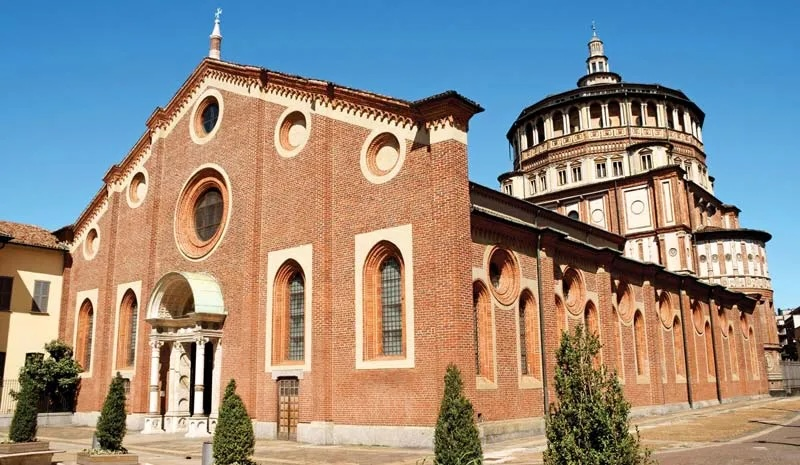
\includegraphics[scale=0.33]{img/churchmilan}
  \caption{Church of Santa Maria delle Grazie in Milan.}
 \label{fig:church-Milan}
\end{figure}

Tartaglia suffered the consequence of the contest. After giving his lectures for a year in Brescia, he was informed that his stipend was not going to be honoured. Even after enumours lawsuit, he could not get any payment. He returned to his previous job in Venice, nursing a huge resentment of Cardano. While for Cardano, it seemed that the oath was hovering over him. In 1560, Cardano's eldest son was accused of poisoning his unfaithful wife and sentenced to death. He was completely devastated by the loss of his son and moved from Milan to Brescia. In 1565, Cardano suffered another blow when his favorite pupil Ferrari was poisoned by his sister. Cardano indulged in gambling and astrology, and he was imprisoned in 1570 for casting the horoscope of Jesus Christ and writting a book in praise of Nero, which was considered heresy by the church. After being released from prison, he moved to Rome and published an autobiography in the last year of his life. In the autobiography, he repeatedly mentioned the pain of losing his son and boasted about his achievements but only briefly mentioned Tartaglia in one sentence. The story here mainly comes from Tartaglia's \emph{New Problems and Inventions} and the letters between him, the intermediary bookseller, Cardano, and Ferrari.

\begin{figure}[htbp]
 \centering
 \subcaptionbox{Tartaglia \label{fig:tartaglia}}{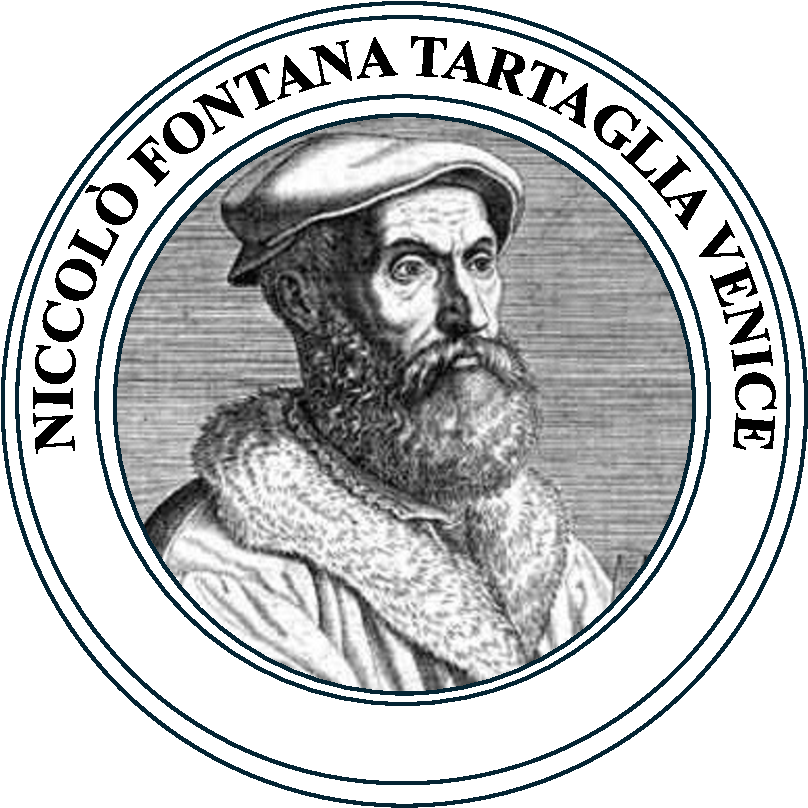
\includegraphics[scale=0.35]{img/tartaglia-coin}}
 \subcaptionbox{Cardano \label{fig:cardano}}{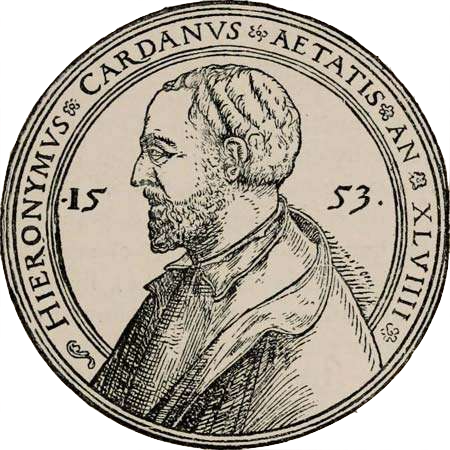
\includegraphics[scale=0.3]{img/Cardano}}
 \caption{Tartaglia and Cardano.}
\end{figure}

We call the formula to the cubic equation the Cardano-Tartaglia formula, or simply the Cardano formula. Besides that, Tartaglia also published a book on ballistics in 1546, which was the first to provide ballistic tables. In 1543, he was the first to translate Euclid's \emph{Elements} into Italian and publish it. He also translated some of Archimedes's works into Italian. Despite his obvious flaws, Cardano was an encyclopedic scholar. He was the first to give a clinical description of typhus, and his mathematical contributions covered algebra and probability theory. He also invented the universal joint, known as the Cardan shaft. Leibniz commented: \enquote{Despite his flaws, he is a great man; but if it were not for these flaws, he would be incomparable.}

\section{The solution of the cubic}

Different from the common understanding, complex numbers were not discovered in the process of solving quadratic equations but were unexpectedly found when solving cubic equations. In this section, we will derive the Cardano formula using both algebraic and geometric methods.

\begin{figure}[htbp]
  \centering
  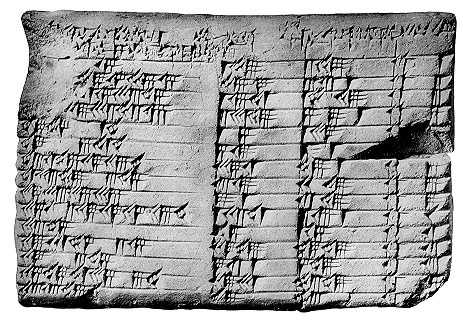
\includegraphics[scale=0.33]{img/plimpton322}
  \caption{The Babylonian clay tablet, Plimpton 322, contains a table of Pythagorean triples, dating from around 2020 BC. It was donated to Columbia University in the 1920s by George Arthur Plimpton.}
 \label{fig:plimpton322}
\end{figure}

\index{Babylonian table of Pythagorean triples}
%% https://personal.math.ubc.ca/~cass/courses/m446-03/pl322/pl322.html

We learned about the early history of quadratic equations from Babylonian clay tablets. As shown in \cref{fig:plimpton322}, this is a clay tablet housed at Columbia University, numbered Plimpton 322. The cuneiform text on this tablet is quite special. German historians of science Neugebauer and Sachs discovered that it was actually a table of Pythagorean triples. Based on the ancient Babylonian numeral system given in Chapter 1, we can easily see that the last column is numbered $1, 2, 3, \dotsc, 15$, with 5, 6, and 15 being damaged. Similarly, the second column from the right is also numbered. The header of the second column from the left indicates the base of a right triangle, which converts to decimal as $119, 3367, 4601, \dotsc, 1771, 56$, with two errors and the last number 56 being damaged. The header of the third column from the left indicates the hypotenuse of a right triangle, which converts to decimal as $169, 4825, 6649, \dotsc, 3229, 106$, with the last number also having an error and being damaged. The numbers in the first column from the left are the most difficult to decipher because the Babylonians had not yet used zero or decimal points by that time. Nevertheless, scientists deciphered it and converted it to decimal numbers as $1.9834\dotso, 1.94916\dotso, 1.9188\dotso$ until $1.43024\dotso, 1.38716\dotso$. The decimals converted from Sexagesimal fractions usually do not terminate (see \cref{thm:finite-decimal}), hence there are ellipses. Denote the base of a right triangle by $w$, the hypotenuse by $d$, and the height by $h$, scientists found that the numbers in the first column are $\dfrac{d^2}{h^2}$, which equals $\dfrac{d^2}{d^2 - w^2}$ according to the Pythagorean theorem. For example, for the first row: $d = 169$ and $w = 119$, we can calculate:

\[
\frac{d^2}{d^2 - w^2} = \frac{169^2}{169^2 - 119^2} = 1.9834\dotso
\]

%% https://engelsbergideas.com/notebook/the-brilliance-of-babylonian-mathematics/
Which is exactly the number in the first column. This table evidently shows that the Babylonians were aware of the Pythagorean theorem (though without a proof to the theorem) and applied it to calculations. As more cuneiform tablets were unearthed, scientists also found \enquote{exercises} related to the Pythagorean theorem. One problem states, \enquote{Given the area and the diagonal of a rectangle, find the lengths of the two sides of the rectangle.} This typical land measurement problem is equivalent to solving the system of equations:

\[
\begin{cases}
  ab = s \\
  a^2 + b^2 = d^2
\end{cases}
\]

\index{geometric solution to the quadratic equations}
where $s$ is the area and $d$ is the diagonal. By substituting $b = \dfrac{s}{a}$ into the second equation, we get a quadratic equation in terms of $a^2$, which is $(a^2)^2 - d^2 a^2 + s^2 = 0$. Since there was no algebraic symbols at that time, the Babylonians described the process of solving quadratic equations in words. Prior to the quadratic formula, we usually learn the \enquote{completing the square} method in school, which is essentially an algebraic solution. The Arabic mathematician Al-Khwarizmi, in his book \emph{The Compendious Book on Calculation by Completion and Balancing}\footnote{The original Arabic title is \emph{Al-Kitab al-Mukhtasar fi Hisab al-Jabr wal-Muqabala}, see \cref{sec:Khwarizmi}}, also followed the Greek tradition, providing geometric explanation for quadratic equations. If $a \ne 0$, we can transform the general quadratic equation $ax^2 + bx + c = 0$ into a form where the coefficient of the quadratic term is 1, and move the constant term to the right side, obtaining $x^2 + \dfrac{b}{a}x = -\dfrac{c}{a}$. Let $p = \dfrac{b}{a}$ and $q = -\dfrac{c}{a}$, we shall solve the equation $x^2 + px = q$ using geometric method. If $p > 0$, \cref{fig:quadratic1} illustrates the geometric interpretation of the left side of the equation. The term $q$ corresponds to the area of a square with side length $x$ plus the area of a rectangle with length $p$ and width $x$.

\begin{figure}[htbp]
  \centering
  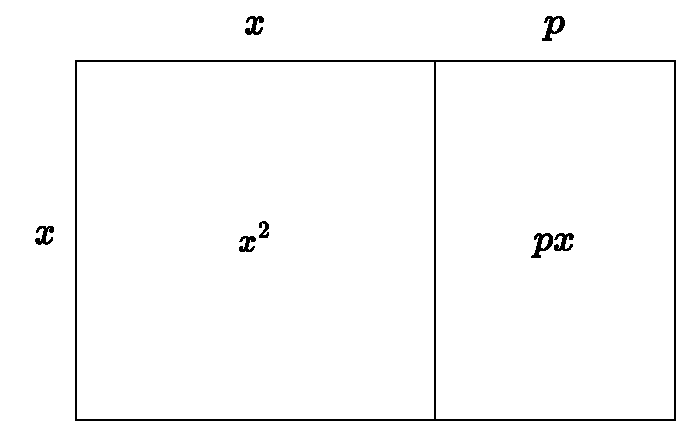
\includegraphics[scale=0.5]{img/quadratic1}
  \caption{geometric interpretation of $x^2 + px$: the sum of a square and a rectangle.}
 \label{fig:quadratic1}
\end{figure}

\index{completing the square}
The method of completing square involves cutting the rectangle into two smaller rectangles of equal length $\dfrac{p}{2}$ and width $x$ (see the left side of \cref{fig:quadratic2}), then moving one to the bottom, and adding a small square with side length $\dfrac{p}{2}$ (the black square on the right side of \cref{fig:quadratic2}) to form a larger square with side length $x + \dfrac{p}{2}$. The white areas in both diagrams are equal, which means:

\begin{align*}
 \left(x + \frac{p}{2}\right)^2 &= q + \left(\frac{p}{2}\right)^2 &&\text{sum of white and black areas} \\
 x + \frac{p}{2} &= \pm \sqrt{q + \left(\frac{p}{2}\right)^2} &&\text{taking square root on both sides} \\
 x &= -\frac{p}{2} \pm \sqrt{q + \frac{p^2}{4}} \\
 x &= -\frac{b}{2a} \pm \sqrt{-\frac{c}{a} + \frac{b^2}{4a^2}} &&\text{substituting} p = \frac{b}{a}, q= -\frac{c}{a} \text{back} \\
 x &= \frac{-b \pm \sqrt{b^2 - 4ac}}{2a}
\end{align*}

\begin{figure}[htbp]
  \centering
  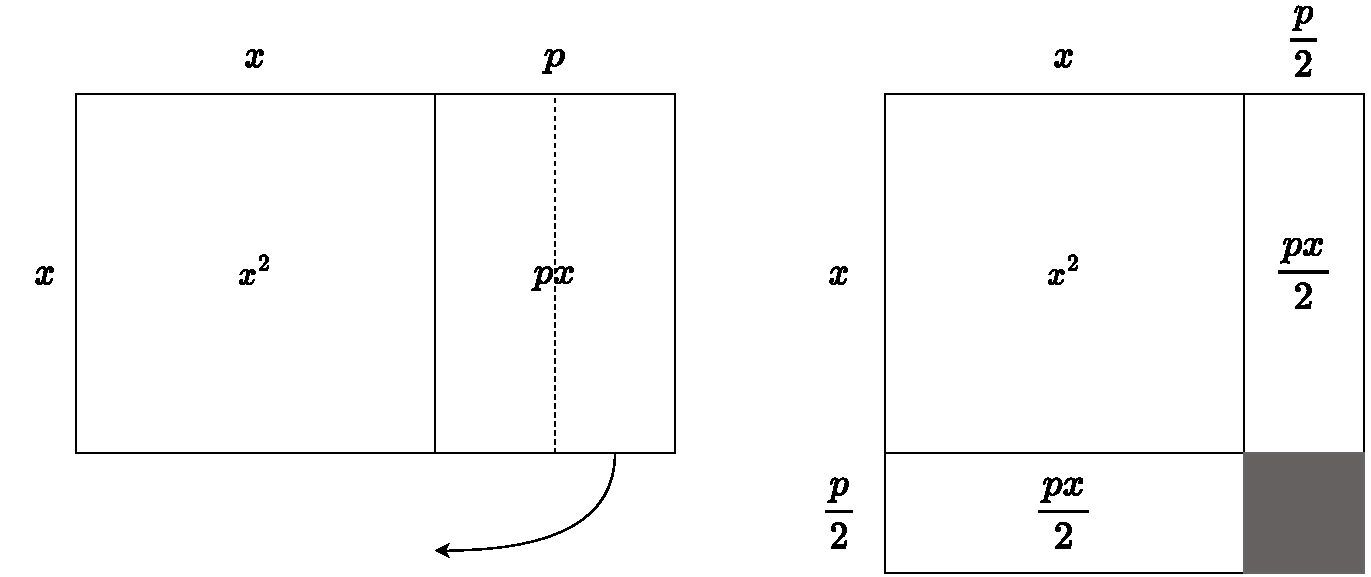
\includegraphics[scale=0.5]{img/quadratic2}
  \caption{geometric interpretation of $x^2 + px$: the sum of a square and a rectangle.}
 \label{fig:quadratic2}
\end{figure}

\index{Cardano formula}
This is the formula for solving quadratic equations. However, during Al-Khwarizmi's living time, negative numbers were not accepted, so when the linear term is negative, a geometric interpretation of $x^2 - px = q$ is needed; when the constant term is negative, a geometric interpretation of $x^2 - q = px$ is needed (see \cref{qn:geometric-quadratic}). Cardano followed this tradition in \emph{Ars magna}, providing both algebraic solutions and geometric interpretations for cubic equations. We first introduce the algebraic solution. For a general cubic equation $a_3x^3 + a_2x^2 + a_1x + a_0 = 0, a_3 \ne 0$, first divide both sides by $a_3$ to make the coefficient of the cubic term to be 1, obtaining $x^3 + \dfrac{a_2}{a_3} x^2 + \dfrac{a_1}{a_3} x + \dfrac{a_0}{a_3} = 0$. Renaming the coefficients as $x^3 + ax^2 + bx + c = 0$. By the end of the 14th century, mathematicians in Florence discovered that by substituting $x = y - \dfrac{a}{3}$, the quadratic term can be eliminated:

\begin{align*}
(y - \frac{a}{3})^3 + a(y - \frac{a}{3})^2 + b(y - \frac{a}{3}) + c &= 0  \\
y^3 -\cancel{ay^2} + \frac{a^2}{3}y - \frac{a^3}{27} + \cancel{ay^2} - \frac{2a^2}{3}y + \frac{a^3}{9} + by - \frac{ab}{3} + c &= 0 && \text{binomial expansion} \\
y^3 + (b - \frac{a^2}{3})y + \frac{2a^3}{27} - \frac{ab}{3} + c &= 0 \\
y^3 + py + q &= 0
\end{align*}

where $p = b - \dfrac{a^2}{3}$ and $q = c + \dfrac{2a^2}{27} - \dfrac{ab}{3}$. As people rejected negative numbers at that time, there are three forms of cubic equations without the quadratic term depending on the signs of $p$ and $q$:

\begin{align}
y^3 + py &= q \label{eq:cubic-linear} \\
     y^3 &= py + q \label{eq:cubic-complex} \\
y^3 + q &= py
\end{align}

What Ferro discovered was the solution to \cref{eq:cubic-linear}, while the solution to \cref{eq:cubic-complex} directly led to the discovery of complex numbers. Let's take $y^3 = py + q$ as an example to derive the formula for solving cubic equations. Let $y = u + v$, then the left side of the equation becomes:

\begin{align*}
y^3 = (u + v)^3 &= u^3 + 3u^2v + 3uv^2 + v^3 && \text{binomial expansion} \\
  &= u^3 + v^3 + 3uv(u + v) \\
  &= u^3 + v^3 + 3uvy && \text{substitute} y = u + v \\
  &= (3uv)y + (u^3 + v^3) = py + q
\end{align*}

equating the coefficients of $y$ and the constant terms, we get:

\[
\begin{cases}
  3uv = p \\
  u^3 + v^3 = q
\end{cases}
\]

This is a system of two equations in terms of $u$ and $v$. From the first equation, we can express $v$ as $v = \dfrac{p}{3u}$, then substitute it into the second equation to get:

\[
u^3 + (\frac{p}{3u})^3 = q
\]

It is acutally a quadratic equation in terms of $u^3$, that is, $(u^3)^2 - qu^3 + (\dfrac{p}{3})^3 = 0$. Applying the quadratic formula solves for $u^3$:

\[
u^3 = \frac{q}{2} \pm \sqrt{\left(\frac{q}{2}\right)^2 - \left(\frac{p}{3}\right)^3}
\]

Since $u$ and $v$ are symmetric in above system, $v^3$ must have the same form. Let them take these two roots respectively:

\[
\begin{dcases}
u^3 = \dfrac{q}{2} + \sqrt{\left(\dfrac{q}{2}\right)^2 - \left(\dfrac{p}{3}\right)^3} \\
v^3 = \dfrac{q}{2} - \sqrt{\left(\dfrac{q}{2}\right)^2 - \left(\dfrac{p}{3}\right)^3}
\end{dcases}
\]

\index{Cardano formula}
They satisfy $u^3 + v^3 = q$. Finally, since $y = u + v$, we obtain the root of the equation:

\be \label{eq:cardano}
y = u + v = \sqrt[3]{\frac{q}{2} + \sqrt{\left(\frac{q}{2}\right)^2 - \left(\frac{p}{3}\right)^3}} + \sqrt[3]{\frac{q}{2} - \sqrt{\left(\frac{q}{2}\right)^2 - \left(\frac{p}{3}\right)^3}}
\ee

\index{geometric solution to cubic equations} \label{sec:geometric-cubic-solution}
This is the Cardano formula for solving cubic equations. We can further find the unknown $x$ using $x = y - \dfrac{a}{3}$. We will next solve the cubic equation $y^3 + py = q$ using geometric methods. As shown in \cref{fig:cube-decompose}, cut a large cube with side length $r$ into 5 parts: a small cube with side length $r-s$ at the lower left front corner; a small cube with side length $s$ at the upper right back corner; and three rectangular prisms with length $r$, width $r-s$, and height $s$, located at the upper left, lower right front, and lower right back corners respectively. The volume of the large cube equals the sum of the volumes of these 5 parts, that is:

\begin{figure}[htbp]
  \centering
  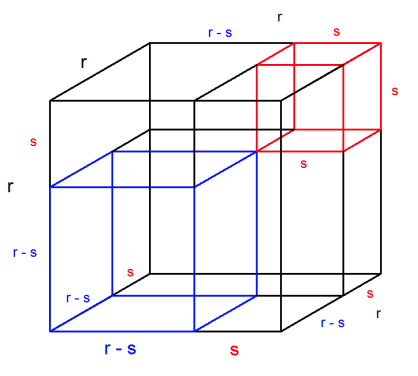
\includegraphics[scale=0.4]{img/cube-decompose}
  \caption{A cube with side length of $r$ consists of 5 parts.}
 \label{fig:cube-decompose}
\end{figure}

\begin{align*}
r^3 = (r-s)^3 + s^3 + 3rs(r-s)  &&\text{two cubes and three rectangular prisms} \\
(r-s)^3 + 3rs(r-s) = r^3 - s^3
\end{align*}

Let $p = 3rs, q = r^3 - s^3$ and substitute into the above equation: $(r-s)^3 + p(r-s) = q$. Obviously, $y = r - s$ is a solution to the equation $y^3 + py = q$. Therefore, as long as we can find suitable $r$ and $s$ based on $p$ and $q$, we can solve the cubic equation. From $p = 3rs$, we have $s = \dfrac{p}{3r}$, and substituting it into $q = r^3 - s^3$ gives us the equation:

\[
r^3 - (\frac{p}{3r})^3 = q
\]

This is actually a quadratic equation in terms of $r^3$, that is, $(r^3)^2 - qr^3 - (\dfrac{p}{3})^3 = 0$. Using the quadratic formula, we can solve for $r^3$:

\[
r^3 = \frac{q}{2} + \sqrt{\left(\frac{q}{2}\right)^2 + \left(\frac{p}{3}\right)^3}
\]

by $q = r^3 - s^3$, hence,

\[
s^3 = -\frac{q}{2} + \sqrt{\left(\dfrac{q}{2}\right)^2 + \left(\dfrac{p}{3}\right)^3}
\]

\index{Cardano formula}
And as $y = r - s$:

\[
y = r - s = \sqrt[3]{\frac{q}{2} + \sqrt{\left(\frac{q}{2}\right)^2 + \left(\frac{p}{3}\right)^3}} + \sqrt[3]{\frac{q}{2} - \sqrt{\left(\frac{q}{2}\right)^2 + \left(\frac{p}{3}\right)^3}}
\]

Comparing this with the Cardano formula derived from algebraic methods, \cref{eq:cardano}, we can see that the only difference is the sign of $p$. This is because in the equations $y^3 + py = q$ and $y^3 = py + q$, the sign of $p$ is opposite. Let's apply the Cardano formula to the equation $x^3 = 6x + 9$.

\begin{align*}
x &= \sqrt[3]{\frac{9}{2} + \sqrt{\left(\frac{9}{2}\right)^2 - \left(\frac{6}{3}\right)^3}} + \sqrt[3]{\frac{9}{2} - \sqrt{\left(\frac{9}{2}\right)^2 - \left(\frac{6}{3}\right)^3}} \\
  &= \sqrt[3]{\frac{9}{2} + \sqrt{\frac{81 - 32}{4}}} + \sqrt[3]{\frac{9}{2} - \sqrt{\frac{81 - 32}{4}}} \\
  &= \sqrt[3]{\frac{9}{2} + \frac{7}{2}} + \sqrt[3]{\frac{9}{2} - \frac{7}{2}} \\
  &= \sqrt[3]{8} + \sqrt[3]{1} = 2 + 1 = 3
\end{align*}

It's easy to verify that $3^3 = 27 = 6 \times 3 + 9$. Cardano's formula to the cubic equation is a significant breakthrough in mathematics, and people were eager to use it to solve various problems. However, some equations were perplexing, with the most famous example being $x^3 = 15x + 4$. By observation, $x = 4$ is a solution to the equation: $4^3 = 64 = 60 + 4 = 15 \times 4 + 4$. But the result given by the Cardano formula is:

\begin{align*}
x &= \sqrt[3]{2 + \sqrt{2^2 - 5^3}} + \sqrt[3]{2 - \sqrt{2^2 - 5^3}}  \\
  &= \sqrt[3]{2 + \sqrt{-121}} + \sqrt[3]{2 - \sqrt{-121}}
\end{align*}

\index{Bombelli}
surprisingly, a negative number appears under the square root. When solving quadratic equations, if the discriminant is negative, people can say \enquote{no solution}. But this equation clearly has a solution $x = 4$, which is not \enquote{no solution}. Cardano didn't know how to answer it, and he commented in \emph{Ars magna}: \enquote{These numbers are both subtle and useless.} The breakthrough on this issue was made by the Italian mathematician Rafael Bombelli (1526–1572). Bombelli imagined simplifying $\sqrt[3]{2 \pm \sqrt{-121}}$ into the form $a \pm b\sqrt{-1}$. Then the two terms in the Cardano formula would add up to:

\[
\sqrt[3]{2 + \sqrt{-121}} + \sqrt[3]{2 - \sqrt{-121}} = a + b\sqrt{-1} + a - b\sqrt{-1} = 2a = 4
\]

Hence, $a = 2$. Next is to determine $b$. Bombelli assumed that $(\sqrt{-1})^2 = -1$, cubing both sides:

\begin{align*}
2 + \sqrt{-121} &= (2 + b\sqrt{-1})^3 \\
  &= 8 + 12b\sqrt{-1} - 6b^2 - b^3\sqrt{-1} && \text{binomial expansion} \\
  &= (8 - 6b^2) + (12b - b^3)\sqrt{-1}
\end{align*}

From $2 = 8 - 6b^2$, it follows that $b = \pm 1$; substituting $1$ into $(12b - b^3)\sqrt{-1}$ gives $11\sqrt{-1}$. Squaring it verifies that $(11\sqrt{-1})^2 = -121$. Therefore, we have $\sqrt[3]{2 + \sqrt{-121}} = 2 + \sqrt{-1}$. For $b = -1$, Bombelli further verified by cubing both sides that $\sqrt[3]{2 - \sqrt{-121}} = 2 - \sqrt{-1}$ also holds. He was very pleased with this result and wrote in his book \emph{Algebra}, published in 1572: \enquote{At first, I felt that such treatment was more like sophistry than truth, but I kept searching until I found the proof.}\cite{OMerino-2006} Bombelli's mathematical perspective was far ahead of his time. When people had not yet accepted negative numbers, Bombelli not only correctly defined the rules of operations between positive and negative numbers in \emph{Algebra}, but also provided the calculation rules for complex numbers. He called $\sqrt{-n}$ the \enquote{plus of minus} and $-\sqrt{-n}$ the \enquote{minus of minus}, then wrote\cite{MacTour-Bombelli}:

\begin{quotation}
Plus of minus times plus of minus makes minus [$\sqrt{-n} \times \sqrt{-n} = -n$]

Plus of minus times minus of minus makes plus [$\sqrt{-n} \times -\sqrt{-n} = n$]

Minus of minus times plus of minus makes plus [$-\sqrt{-n} \times \sqrt{-n} = n$]

Minus of minus times minus of minus makes minus [$-\sqrt{-n} \times -\sqrt{-n} = -n$]
\end{quotation}

Bombelli had planned five books of \emph{Algebra}, sadly, he died in 1572 after publishing the first three books. The remaining two were not discovered until 1923 in a library in Bologna, Italy. At that time, people did not believe and accept Bombelli's views, and the mathematical community largely rejected $\sqrt{-1}$. In the following 200 years, even though a few scholars like Wallis attempted to give meaning to complex numbers, most people either doubted or ignored Bombelli's calculation rules. It wasn't until 1770 that Euler still \enquote{proved} in his work that $\sqrt{-2} \times \sqrt{-3} = \sqrt{6}$, which would surprise us today\footnote{Euler actually used the symbol $\sqrt{6}$ to represent the two square roots of 6, $\pm\sqrt{6}$; similarly, $\sqrt{-2}$ represents the two square roots of -2, $\pm\sqrt{-2}$; and $\sqrt{-3}$ represents the two square roots of -3, $\pm\sqrt{-3}$. Thus, Euler's original intention was to express all combinations of $\pm \sqrt{-2} \times \pm \sqrt{-3} = \pm \sqrt{6}$.}. Some people highly praised Bombelli's work; Leibniz said he was \enquote{a master of the art of analysis.} Today, Bombelli is known as \enquote{the father of imaginary numbers.}

\begin{figure}[htbp]
  \centering
  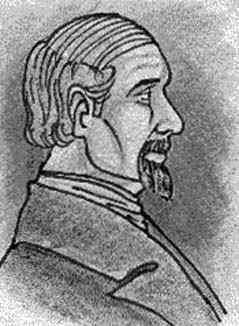
\includegraphics[scale=0.4]{img/Bombelli}
  \caption{Rafael Bombelli (1526 - 1572)}
 \label{fig:Bombelli}
\end{figure}

Bombelli used the form $a + b\sqrt{-1}$. The first person to use this form was Cardano, but he immediately rejected it. In Chapter 37 of \emph{Ars magna}, Cardano presented a problem: divide 10 into two parts such that their product is 40. The system of equations is:

\[
\begin{cases}
x + y = 10 \\
xy = 40
\end{cases}
\]

Represent $y$ as $10 - x$, and substitute it into the second equation to get $x(10 - x) = 40$. Dividing 10 into two parts, the maximum product is $5 \times 5 = 25$, so 40 is impossible (we can also think of it as using a 20 $cm$ rope to form a rectangle, the square with side length 5 has the largest area of 25 $cm^2$). Cardano wrote:

\begin{quotation}
  This is clearly impossible. However, if we divide 10 into two parts of 5, the square is 25. Subtracting 40 from it, if you wish, gives $-15$. By adding and subtracting the square root of $-15$ to 5, we get two numbers whose product is 40. Therefore, these two numbers are $5 + \sqrt{-15}$ and $5 - \sqrt{-15}$. Although it may seem absurd, by cubing both sides of the equation

Dismissing mental tortures, and multiplying $5 + \sqrt{-15}$ by $5 - \sqrt{-15}$, we obtain $25 - (-15)$. Therefore the product is 40. .... and thus far does arithmetical subtlety go, of which this, the extreme, is, as I have said, so subtle that it is useless.
\end{quotation}

\index{imaginary number}
Cardano's method was to divide 10 into two parts, $5 + x$ and $5 - x$, such that their product is 40. Because $(5 + x)(5 - x) = 25 - x^2 = 40$, hence $x^2 = -15$. This leads to the solution $5 \pm \sqrt{-15}$. Due to the irrationality of negative squares, particularly in the application of quadratic equations, Cardano and most of his contemporaries abandoned complex solutions. However, Bombelli realized that in  cubic equations, such numbers as intermediate results make sense. The term \enquote{imaginary number} attributes to Descartes. When developing analytic geometry\footnote{Published in the appendix \emph{La Géométrie} of his book \emph{Discours de la méthode}.} in 1637, Descartes corresponded the roots of equations to the intersection points between curves or the zeros of curves with coordinate axes. Although people at that time did not recognize the fundamental theorem of algebra, Descartes had insights that the number of roots of an equation equals its degree. Curves may not intersect with each other, or intersect with the $x$-axis, Facing with such geometrically impossible constructions, Descartes considered their intersection points or zeros as imaginary. The term \enquote{imaginary} also has the meaning of being imagined in English. Descartes wrote \enquote{, For any equation, one can imagine as many roots as its degree, but in many cases, these roots correspond to values that do not exist.}

\index{i as imaginary unit}
We use the symbol $i$ as the imaginary unit today. This symbol was chosen by Euler. It is the first letter of \enquote{imaginary}. Descartes' opinion reflected the view of most people at that time. Mathematicians did not like the terms indicating fiction and imagination. One reason is that $\sqrt{-n}$ brought confusion and ambiguity. For example, does the common operation rule $\sqrt{ab} = \sqrt{a}\sqrt{b}$ still hold? Some pointed out such a problem:

\begin{align*}
70 &= \sqrt{4900} = \sqrt{(-100)\times(-49)} = \sqrt{-100}\sqrt{-49} \\
   &= (10i)(7i) = 70 \times (-1) = -70
\end{align*}

$70 = -70$ is absurd (see \cref{qn:sqrt-of-product}). Cauchy, known as the father of complex analysis,  suggested rejecting the symbol $\sqrt{-1}$, and Gauss was also dissatisfied with $i$, suggesting a new name. But his suggestion came too late, as $i$ had already been widely used and continues to be used today.

\section{Geometric interpretation}

Nobody will accept complex numbers unless they have a clear meaning, that is natural, convincing, and able to solve real problems. In 1673, Wallis, a pioneer of calculus attempted to give a geometric interpretation of complex numbers. Wallis, who invented the number line, tried to use it to solve the equation $x^2 + 2bx + c^2 = 0$. The two roots are $x_{1,2} = -b \pm \sqrt{b^2 - c^2}$. As shown in \cref{fig:wallis1}, Wallis marked $-b$ on the number line and constructed two right triangles on either side with height $c$ and hypotenuse length $b$. By Pythagorean theorem, the length of other leg is $a = \sqrt{b^2 - c^2}$. Therefore, on either side of the point $-b$, at a distance of $a$, are the two roots $x_{1,2}$.

\begin{figure}[htbp]
  \centering
  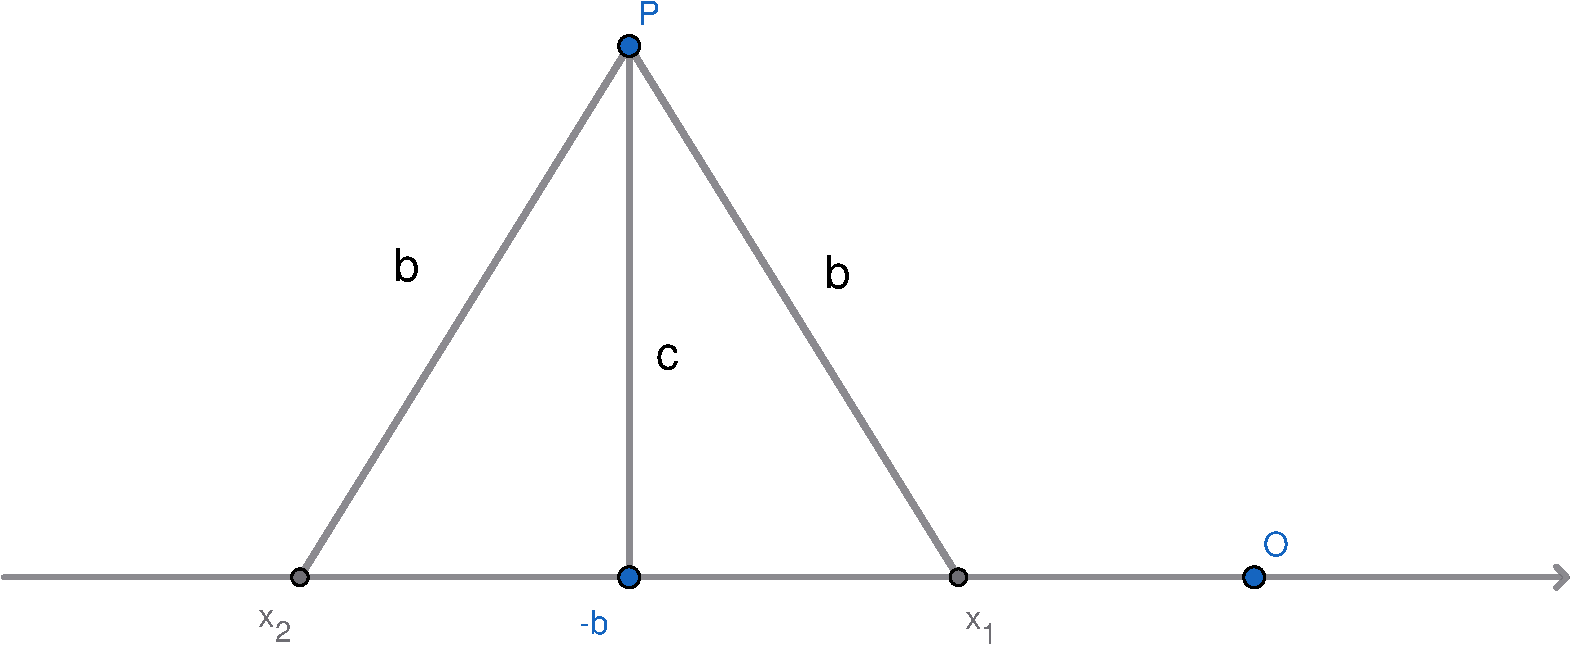
\includegraphics[scale=0.33]{img/wallis1}
  \caption{Roots $x_{1,2} = -b \pm \sqrt{b^2 - c^2}$ on the number line.}
 \label{fig:wallis1}
\end{figure}

Everything is fine so far. Then Wallis kept increasing the value of $c$, and the two roots $x_{1,2}$ got closer and closer to the point $-b$. When $c = b$, the two roots coincide. What if we keep increasing $c$? Wallis drew a picture as shown in \cref{fig:wallis2}.

\begin{figure}[htbp]
  \centering
  \subcaptionbox{Where Wallis marked $-b \pm i\sqrt{c^2-b^2}$. \label{fig:wallis2}}{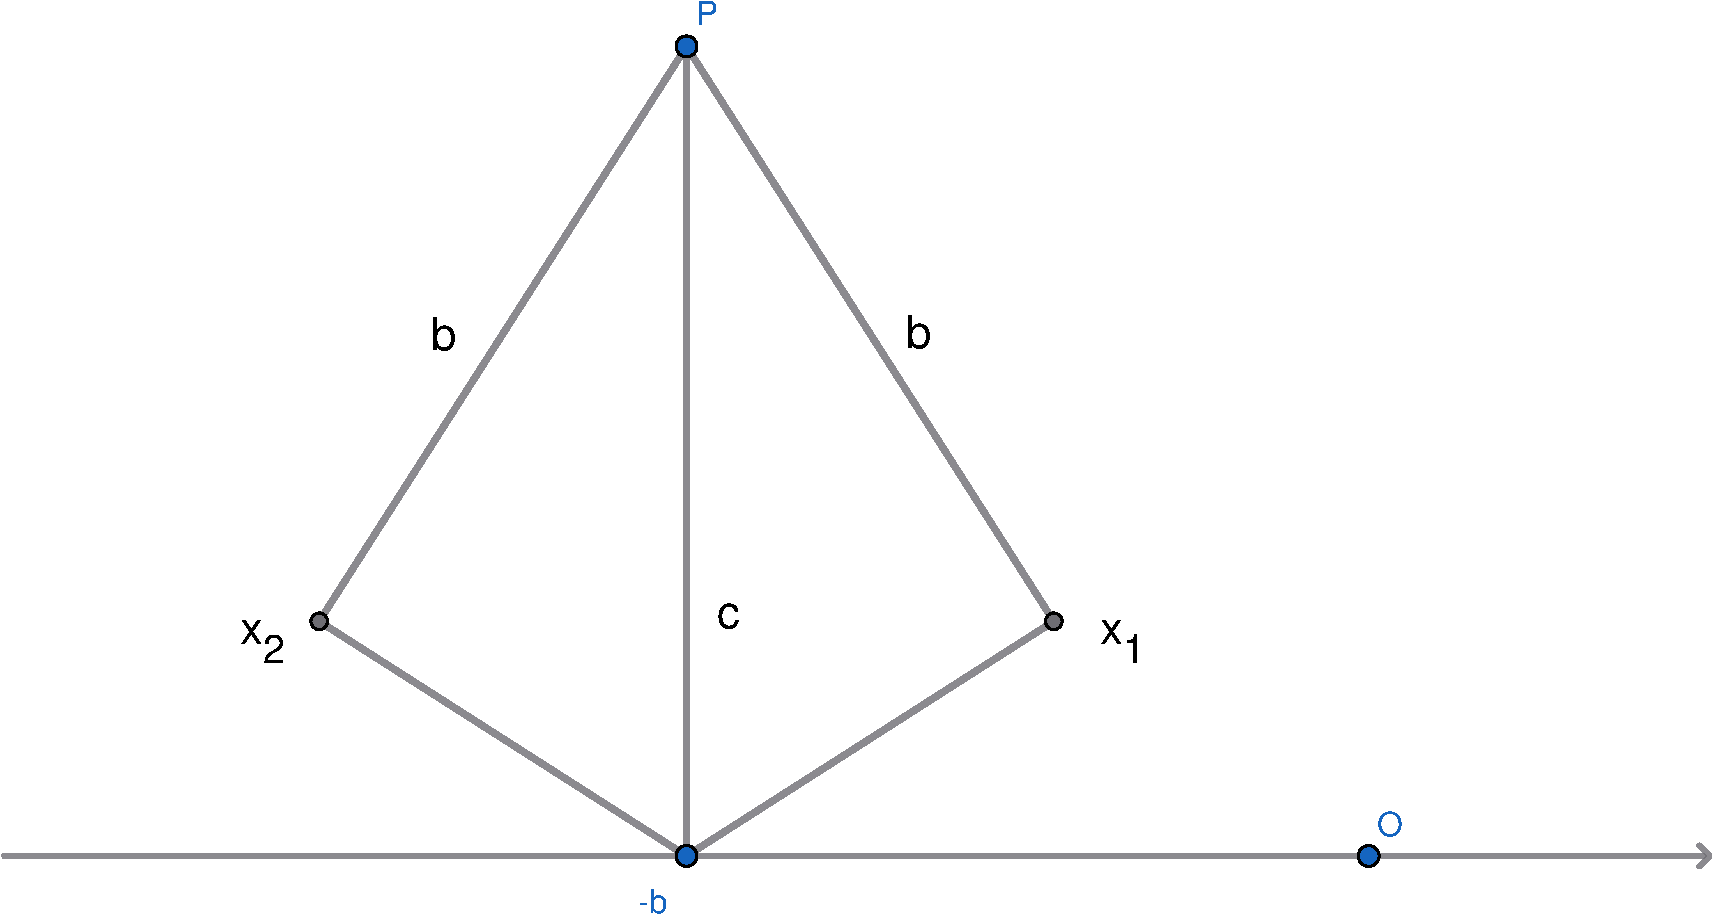
\includegraphics[scale=0.33]{img/wallis2}}
  \subcaptionbox{The location of $-b \pm i\sqrt{c^2-b^2}$ in the complex plane. \label{fig:wallis3}}{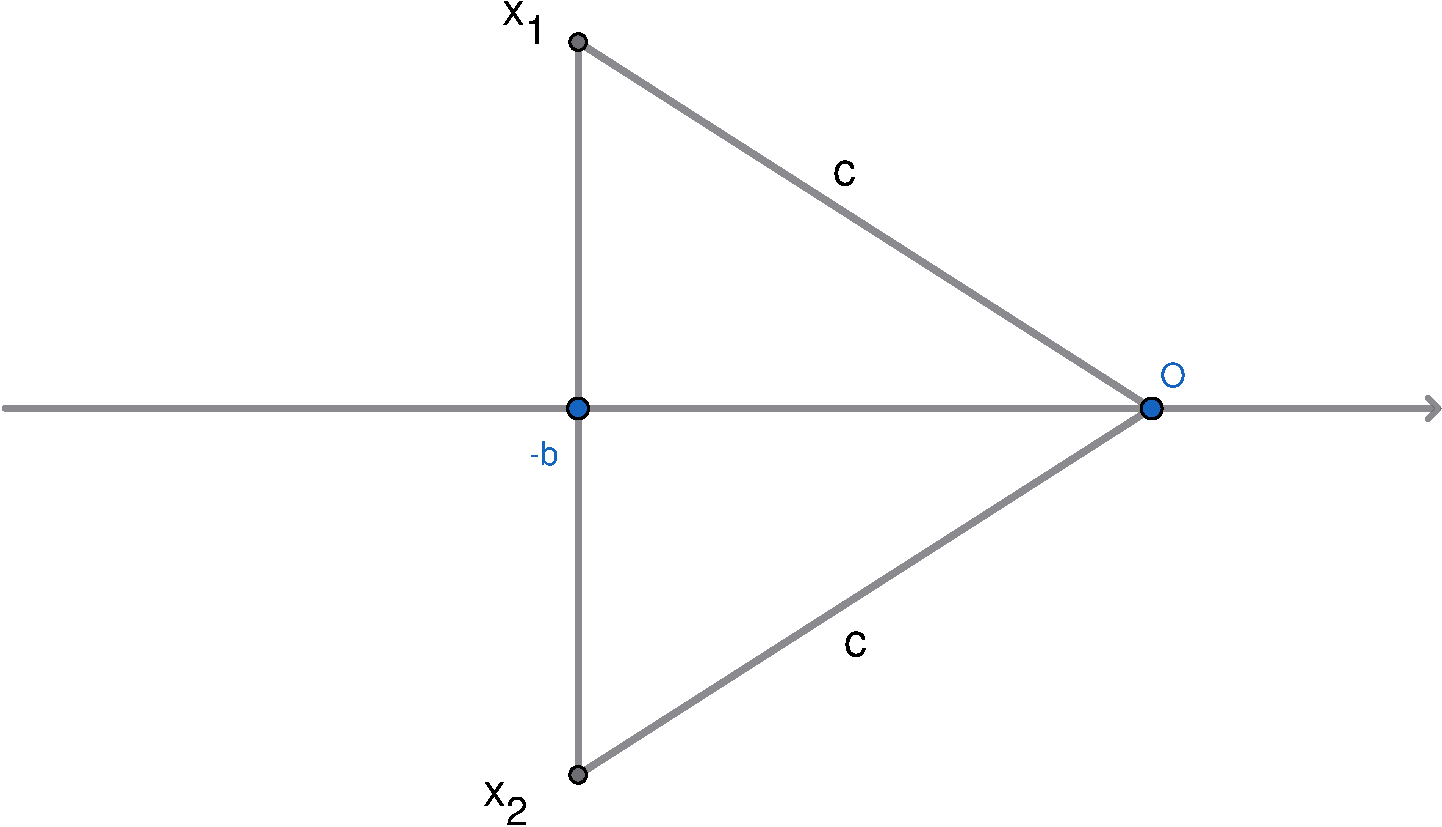
\includegraphics[scale=0.33]{img/wallis3}}
  \caption{Roots of $x^2 + 2bx + c^2 = 0$ when $c > b$.}
\end{figure}

\index{Wessel}
It's almost correct. Wallis thought that at this point, $c$ becomes the hypotenuse, one leg is $b$, and the other leg is $\sqrt{c^2 - b^2}$, but they are still on either side of the point $-b$. In fact, if Wallis had just swapped the left and right sides to up and down, he could have touched the complex plane. It's really a pity. The first person in history who successfully gave the geometric interpretation to complex numbers was Danish-Norwegian mathematician Caspar Wessel (1745–1818). On March 10, 1797, Wessel submitted his work to the Royal Danish Academy of Sciences and Letters, titled \emph{On the Analytical Representation of Direction—An Attempt at Solving Problems in Geometry of Position}. He successfully represented a complex number $a + bi$ as a line segment (i.e., a vector) from the origin to the coordinate $(a, b)$ in a Cartesian coordinate system, and defined algebraic rules for calculations between vectors, including addition and multiplication. Geometrically, the addition rule corresponds to the \enquote{parallelogram} principle; multiplication corresponds to multiplying the lengths of the line segments and adding their  angles with respect to the horizontal axis. Wessel's paper was published two years later. Unfortunately, Wessel's was a surveyor rather than a well-known mathematician, and his paper was written in Danish, which did not attract enough attention at that time. Wessel's name was ignored by most people until about 100 years later in 1895 when his work was reappreciated. Norwegian mathematician Sophus Lie republished Wessel's paper. Even more surprisingly, in 1806, a young man independently rediscovered the complex plane and the geometric meaning of complex numbers, but no one knows his name.

\subsection{The mysterious young man}
\index{Argand}
In the autumn of 1806, a young man knocked on the door of Adrien-Marie Legendre, a member of the Paris Academy. He was very nervous. Legendre was considered one of the best mathematicians and the successor of Lagrange. After Napoleon rebuilt the Academy, he appointed Legendre as the head of the mathematics section and the chief examiner of France's highest institution, the École Polytechnique. The young man made a brief self-introduction, and due to his nervousness, he even forgot to mention his name. He respectfully handed Legendre a manuscript and asked him to review. The young man did not explain the purpose in detail, but when asked about the content of the paper, he immediately became excited. enquote{this is a treatise on imaginary numbers. I found them actually meaningful, as real as other numbers! As long as we treat them as line segments, we will find...} Legendre was skeptical about the young man's rambling. He had to interrupt: \enquote{I am very busy right now, but I promise to read your paper when I have time. Let's stop here for today.} Before the door closed, the young man pleaded again: \enquote{Sir, I am very much looking forward to your criticism and suggestions.}

Legendre soon forgot about this encounter. He was busy with his research and the affairs of the Academy. Until a few weeks later, Legendre happened to see a few sheets of paper on his desk, titled \emph{A Treatise on a Method of Representing Imaginary Numbers in Geometric Constructions}. Who sent this? Oh, I remember, what was that young man's name? I can't recall it, but anyway, Legendre read on. To his surprise, once started reading, he was immediately impressed by the innovative ideas, the smooth and flowing arguments, the solid calculations, and the precise conclusions that perfectly combined numbers, geometry, and trigonometry. Legendre decided to contact this young man immediately and have an in-depth discussion with him. However, he searched through the paper but could not find any name or address. How could this be? Maybe this young man will come again in a few days? Legendre decided to wait. Day after day, from late autumn to early winter, the first snow had already fallen in Paris. But the young man never showed up again. Will this young man publish his paper directly in a journal? Then I can find him for discussion. Legendre went to the library to check various mathematical journals from the past few months, but was disappointed again. Maybe the young man was discouraged by Legendre's response that day and gave up on this research. On November 2, Legendre sent this paper to his friend and collaborator François Français, with a brief comment praising the young man for his love of scholarship without seeking fame, and noting that although it was a draft, it was sufficiently innovative.

François Français mainly studied partial differential equations, and although his work was often praised by the French Academy, he rarely published during his lifetime. After François Français's death in 1810, his brother Jacques Français discovered this memoir on complex numbers while organizing his papers. He published it in September 1813 under the title \emph{New Principles of Geometry of Position and an Explanation of the Symbol of Imaginary Numbers}. Jacques Français showed true scholarly spirit; he did not claim this achievement as his own. At the end of the paper, he pointed out that these ideas came from an unknown mathematician and he asked that the mathematician should make himself known so that he might receive the credit for his ideas. Soon after the article by Jacques Français appeared in Gergonne's famous journal\emph{Annales de mathématiques}, a person named Argand responded that he was that unknown author and sent a slightly modified manuscript titled \emph{A Treatise on a Method of Representing Imaginary Numbers in Geometric Constructions}. Argand added new applications in it. This already dramatic event then attracted the attention of many mathematicians: Jacques Français, Argand, and Servois engaged in a heated discussion in \emph{Annales de mathématiques}. Servois believed that complex numbers must be treated with pure algebra, while Jacques Français and Argand advocated for the effectiveness of geometric representation. Argand then demonstrated the power of geometric representation of complex numbers - he proved the fundamental theorem of algebra. From today's perspective, although there are some flaws, it is one of the clearest and most elegant proofs. Argand's work was ahead of its time, but unfortunately, we do not know who he really is! He only signed as \enquote{Argand} in all his papers, but not the full name.Which one among many people named Argand is he? We only know that he appeared in Paris in 1806, and the paper published in 1813 was sent from Paris. Some speculate that he might be Jean Robert Argand, an accountant and amateur mathematician living in Paris, but the age does not match. In 1806, Legendre described him as a \emph{young} man, but Jean Robert Argand was already 38 years old at that time\cite{MacTour-Argand}.

\index{Argand diagram}
Our story mainly comes from the letters between Legendre and François Français, and the paper by Jacques Français. To commemorate Argand's achievements, today we call \cref{fig:Argand-diagram} the \enquote{Argand diagram}, which appears in classrooms around the world\cite{Weisstein-2025}.

\begin{figure}[htbp]
  \centering
  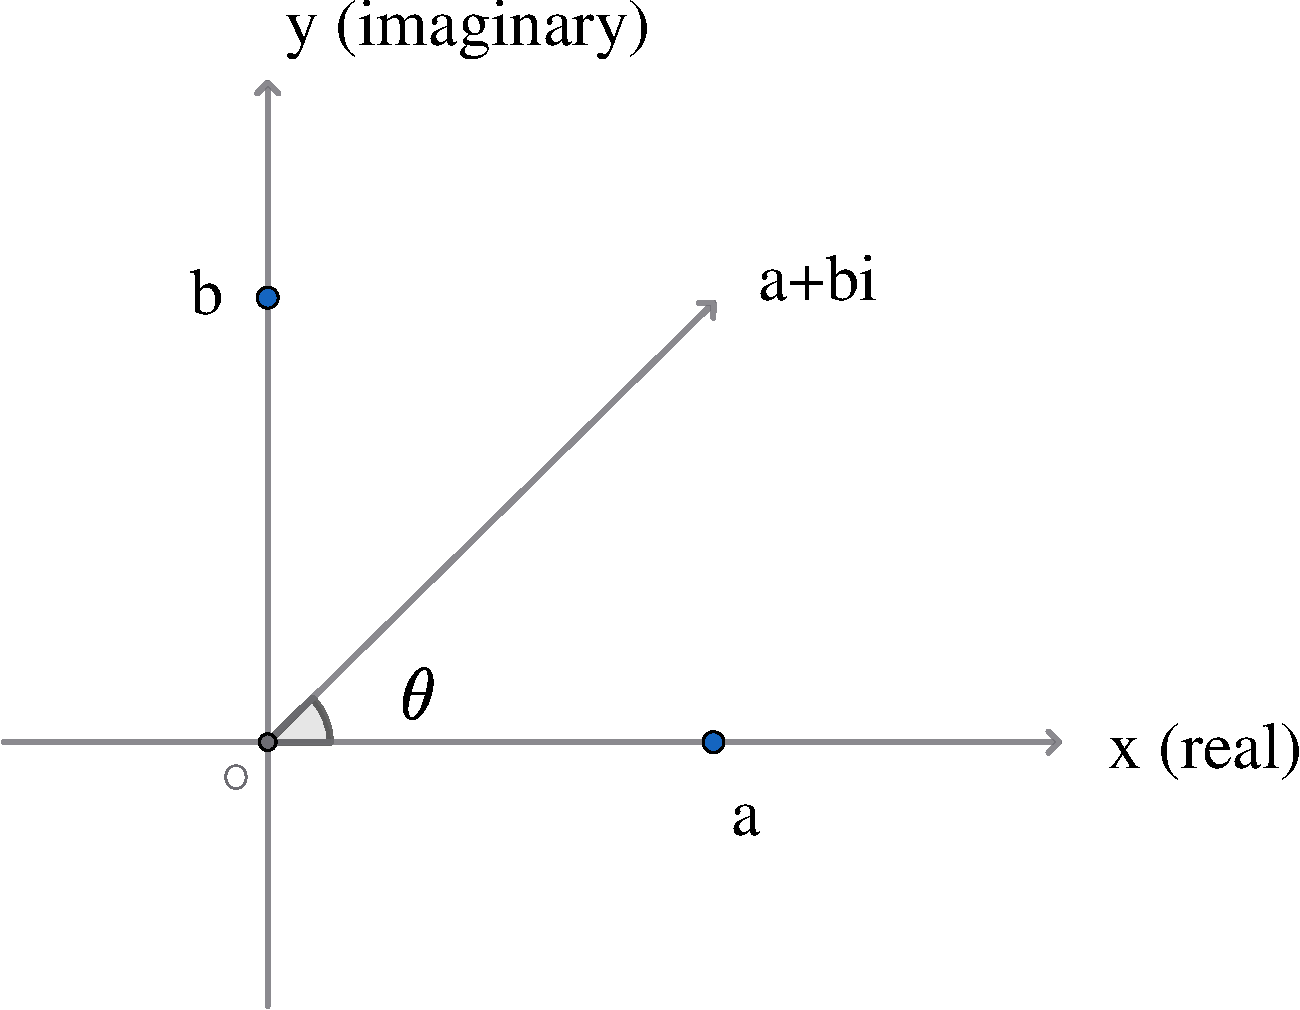
\includegraphics[scale=0.33]{img/argand-diagram}
  \caption{Argand diagram}
 \label{fig:Argand-diagram}
\end{figure}

\subsection{The geometric interpretation of complex numbers}
\index{The geometric interpretation of complex numbers}
A picture is worth a thousand words. We can immediately see from the Argand diagram that a complex number $z$ consists of two parts: the real part $a$ and the imaginary part $bi$. The imaginary axis creatively extends vertically upwards, and the real axis and the imaginary axis are perpendicular to each other, forming the complex plane. A complex number is represented as a vector from the origin to the point with coordinates $(a, b)$ in the complex plane. Drawn as a line segment with an arrow, this vector is $a + bi$. The imaginary unit $i$ is not any real number because it is not on the real axis at all. If we say that any number $a$ on the real axis multiplied by $-1$ corresponds to a \enquote{turning back}, becoming a negative number $-a$ pointing to the other side, then multiplying $a$ by $i$ corresponds to \enquote{turning left by $90\degree$}, becoming $ai$ on the imaginary axis; multiplying by $i$ again corresponds to \enquote{turning left by another $90\degree$}, returning to the real axis pointing to the other side as $-a$. Two turns of $90\degree$ correspond to a turn of $180\degree$, which perfectly explains why $i^2 = -1$. We can immediately see from the Pythagorean theorem that the length of the line segment represented by the vector $a + bi$ is $r = \sqrt{a^2 + b^2}$, which is called the modulus of the complex number $z$, denoted as $|z|$. The angle between the vector and the real axis is called the argument of the complex number, denoted as $\arg(z)$. From the definition of trigonometric functions, we immediately know that the real part and imaginary part of a complex number can be expressed as: $a = r\cos\theta, b = r\sin\theta$, thus there are two equivalent representations for a complex number:

\[
a + bi = r\cos\theta + ir\sin\theta = r(\cos\theta + i\sin\theta)
\]

Argand diagram algo gives a clear interpretation to the multiplication of complex numbers: \index{complex number multiplication}

\begin{align*}
z_1z_2 &= r_1(\cos\theta_1 + i\sin\theta_1) \cdot r_2(\cos\theta_2 + i\sin\theta_2) \\
  &= r_1r_2[\cos\theta_1\cos\theta_2 - \sin\theta_1\sin\theta_2 + i(\sin\theta_1\cos\theta_2 + \cos\theta_1\sin\theta_2)] && \text{expanding }, i^2 = -1 \\
  &= r_1r_2[\cos(\theta_1 + \theta_2) + i\sin(\theta_1 + \theta_2)] && \text{sum of angles formulas}
\end{align*}

\label{sec:proof-to-machin}
Thus when multiplying two complex numbers, we multiply their moduli and add their arguments. The mathematician Abraham de Moivre (1667–1754) multiplied two complex numbers with modulus 1 and the same argument to get:

\[
(\cos \theta + i\sin \theta)^2 = \cos (\theta + \theta) + i\sin (\theta + \theta) = \cos 2\theta + i\sin 2\theta
\]

\index{de Moivre's formula}
Further, multiplying $n$ such complex numbers together gives the famous de Moivre's formula:

\be \label{eq:de-Moivre}
(\cos \theta + i\sin \theta)^n = \cos n\theta + i\sin n\theta
\ee

Argand's geometric interpretation of complex numbers is a perfect example of the integration of numbers, geometry, vectors, and trigonometry. To demonstrate the power of the combination of numbers and shapes that complex numbers possess, we will give an elegant proof of Machin's formula (see \cref{sec:machin-formula}). People found Leibniz's formula for $\pi$ converges very slow, they found below series converges much faster:

\[
\frac{\pi}{4} = \tan^{-1} \frac{1}{2} + \tan^{-1} \frac{1}{3}
\]

\begin{proof}
 The argument of a complex number $z = a + bi$ is given by $\arg(z) = \tan^{-1}\dfrac{b}{a}$. The right side of the above equation can be seen as the sum of two arguments, which correspond to the complex numbers $z_1 = 2 + i$ and $z_2 = 3 + i$. When multiplying two complex numbers, their arguments add up, that is, $\arg(z_1 z_2) = \arg(z_1) + \arg(z_2)$.

\begin{align*}
z_1 z_2 &= (2+i)(3+i) = (6 - 1) + (2 + 3)i = 5 + 5i \\
arg(5 + 5i) &= arg(2+i) + arg(3+i) && \text{add arguments when multiply complex numbers} \\
\frac{\pi}{4} &= \tan^{-1}\frac{5}{5} = \tan^{-1}\frac{1}{2} + \tan^{-1}\frac{1}{3} && \text{see \cref{fig:machin1}} \qedhere
\end{align*}
\end{proof}

\begin{figure}[htbp]
  \centering
  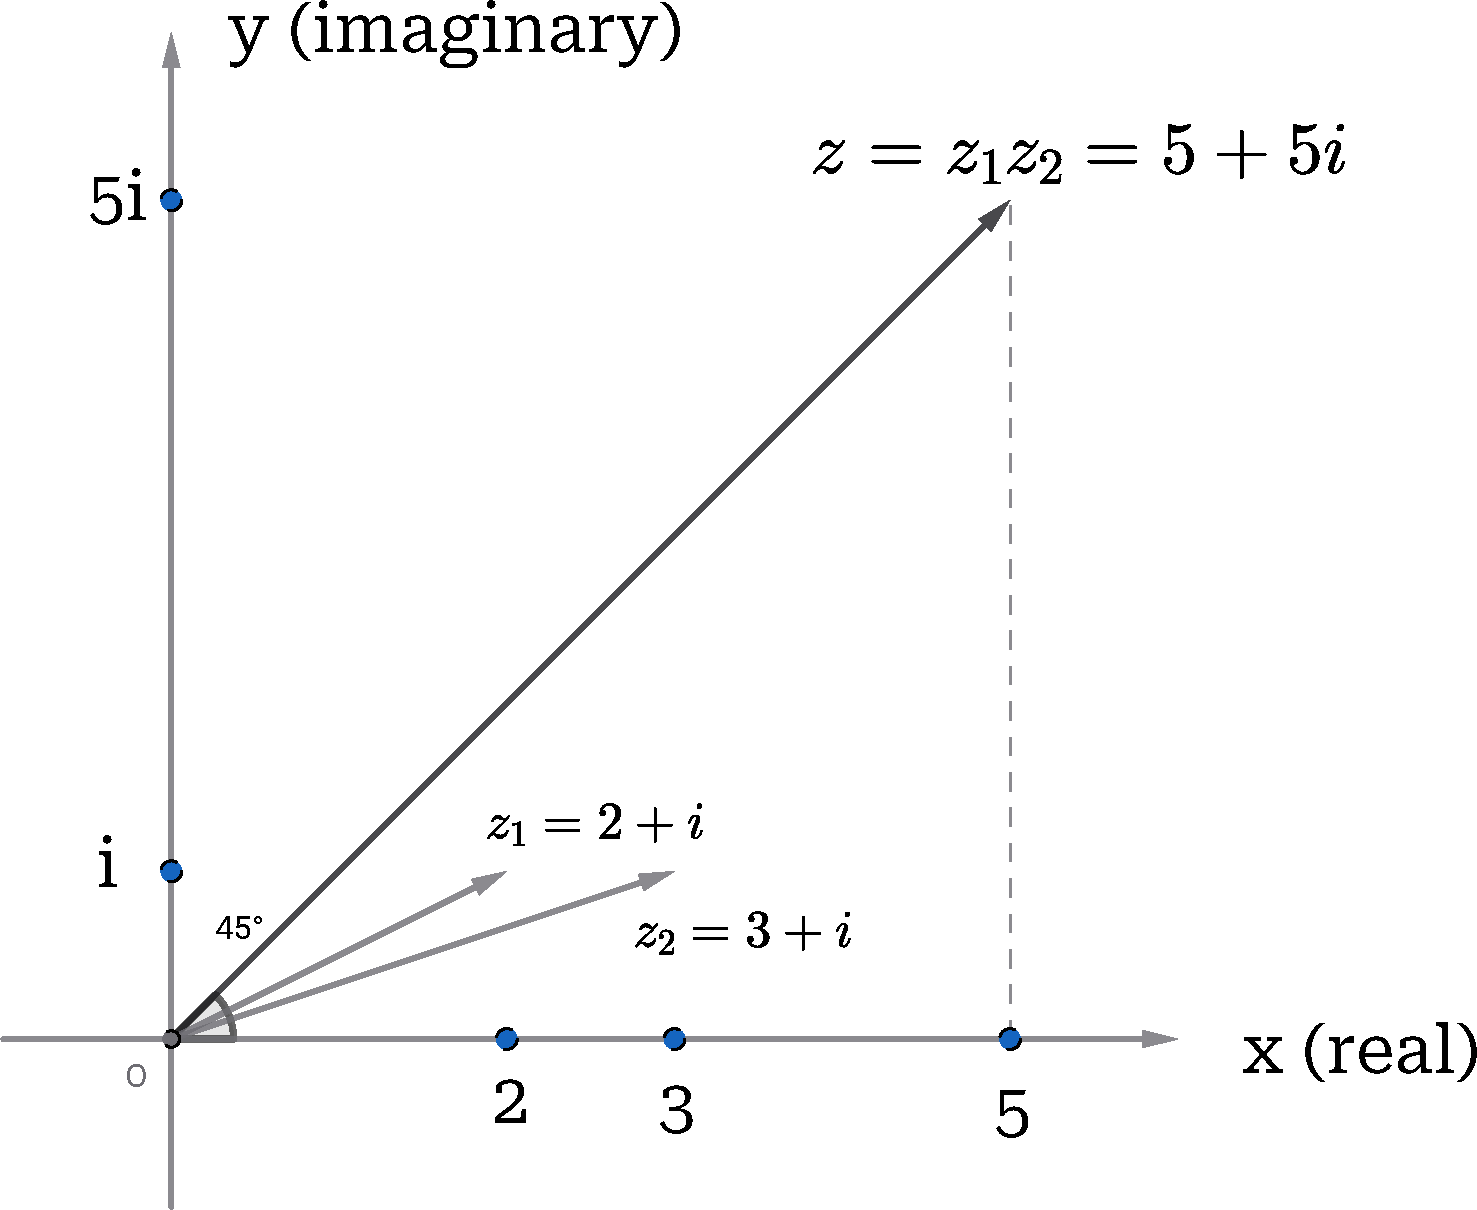
\includegraphics[scale=0.33]{img/machin1}
  \caption{$(2 + i)(3 + i) = 5 + 5i$}
 \label{fig:machin1}
\end{figure}

\index{Machin's formula}
We are going to prove Machin's formula:
\[
\frac{\pi}{4} = 4\tan^{-1} \frac{1}{5} - \tan^{-1} \frac{1}{239}
\]

\begin{proof}
Let $z_1 = 5 + i, z_2 = 239 - i$. The 4 times of the argument of $z_1$ on the right corresponds to the argument of $z_1^4$. We construct the product of,

\begin{align*}
z &= z_1^4z_2 = (5+i)^4(239-i) \\
  &= (25 - 1 + 10i)^2(239 - i) && \text{square of sum} \\
  &= (24^2 - 100 + 480i)(239 - i) && \text{square of sum again} \\
  &= 476 \times 239 + 480 + (480 \times 239 - 476)i && \text{expand} \\
  &= 114244 + 114244i
\end{align*}

The argument of $z$ is exactly $\dfrac{\pi}{4}$.
\end{proof}

\index{Conjugate complex numbers}
This is supposed to be the shortest and most elegant proof of Machin's formula. This proof reveals a geometric property of complex numbers: if a complex number $z = a + bi$ has an argument $\theta$, where $b \ne 0$, then the complex number $a - bi$ has an argument $\tan^{-1}\dfrac{-b}{a} = -\theta$. Let $\overline{z} = a - bi$ be the conjugate of $z$. Thus, dividing by $a + bi$ corresponds to multiplying by $a - bi$ in terms of the angle of rotation. We can conveniently convert division into multiplication using conjugate complex numbers. In particular, since $z\overline{z} = (a + bi)(a - bi) = a^2 + b^2 = |z|^2$, we have:

\[
\frac{1}{z} = \frac{\overline{z}}{z\overline{z}} = \frac{1}{|z|^2}\overline{z}
\]

When the modulus of $z$ is 1, we have $\dfrac{1}{z} = \overline{z}$. For example, for $z = \cos\theta + i\sin\theta$, we immediately know that:

\[
\frac{1}{\cos\theta + i\sin\theta} = \cos\theta - i\sin\theta
\]

All complex numbers on the unit circle satisfy this condition. \cref{qn:trigonometry-of-add} requires us to derive the sum of angles formulas for trigonometric functions using complex number operations.

\subsection{The foundamental theorem of algebra}

When accepting complex numbers, those quadratic equations couldn't be solved before suddenly have solutions. For example, the problem in Cardano's \emph{Ars magna}: two numbers add up to 10 and multiply to 40, that is, $(5 + x)(5 - x) = 40$. Expanding using the difference of squares formula gives $x^2 + 15 = 0$. It has no real solution, but it has two complex roots: $x_{1,2} = \pm i\sqrt{15}$; the polynomial $x^2 + 15$ cannot be factored using real numbers, but it can be factored using complex numbers as $(x + i\sqrt{15})(x - i\sqrt{15})$. Moreover, the three cases that were originally complicated: (1) two distinct real roots, (2) two identical real roots, (3) no real roots, become simple and consistent in complex numbers: any quadratic equation has two complex roots, counting repeated roots as two. Mathematicians are extreme minimalists and perfectionists; no one can resist such an elegant conclusion. What about cubic equations? Quartic equations? And higher degree equations? Descartes discovered a powerful weapon for conquering higher degree equations. He also introduced the notation $x^n$ casually. Before Descartes, people used special terms like \enquote{square} and \enquote{cube} to describe $xx$ and $xxx$, and even had special terms like quartic for \enquote{fourth power} and quintic for \enquote{fifth power}. However, symbols like $xxxx$ and $xxxxx$ were obviously too cumbersome. When Descartes established analytic geometry in 1637, he was the first to introduce notations like $x^3, x^4, x^5$. We see again how important good notation is! In history, the trend of development has been from \enquote{verbal description} $\to$ \enquote{abbreviation} $\to$ \enquote{symbol}, evolving in this direction. Many people are afraid of formulas filled with symbols; memorizing formulas during school is a terrifying memory for most adults. Some people therefore dislike mathematics for life; this is really a misunderstanding and a pity. In fact, mathematics is the least memorization-intensive subject because we can rely on intuition, reason, and aesthetics to derive almost all conclusions. Contrary to many people's feelings, symbols are simpler, easier to understand, and more precise than verbal descriptions. You can compare the verbal description \enquote{the area of the square constructed on one leg of a right triangle plus the area of the square constructed on the other leg equals the area of the square constructed on the hypotenuse} with the algebraic symbol $a^2 + b^2 = c^2$.

\index{Descartes's theorem}
\begin{theorem}[Descartes]
Let $p(x) = a_nx^n + \dotsb + a_1x + a_0$ be a polynomial with $a_n \ne 0$. Then $p(x) = 0$ has a root $x = b$ if and only if $p(x)$ has a factor $x - b$.
\end{theorem}

Descartes's theorem means that if $b$ is a root, then we can factorize the polynomial as $p(x) = (x - b)q(x)$ where the degree of $q(x)$ is less than that of $p(x)$. And this is a necessary and sufficient condition, so the converse is also true. We can conveniently use Descartes's theorem to factorize $x^3 - 1$: clearly, $1$ is a root of the equation $x^3 - 1 = 0$, so $x - 1$ is a factor. Then we use polynomial long division to find:

\[
\polylongdiv{x^3-1}{x-1}
\]

Alternatively, as the sum of the geometric series $1 + x + x^2 + \dotsb + x^{n-1} = \dfrac{x^n - 1}{x - 1}$, we can factorize $x^3 - 1$ as $(x - 1)(x^2 + x + 1)$ without performing polynomial long division.

\begin{proof}
If $x - b$ is a factor of $p(x)$, then $p(x) = (x - b)q(x)$. Substituting $x = b$ gives $p(b) = (b - b)q(b) = 0$, so $b$ is a root.

Conversely, if $x = b$ is a root of $p(x)$, that is, $p(b) = 0$. We can extend the division algorithm with remainder to polynomials. Dividing $p(x)$ by $x - b$, we have $p(x) = (x - b)q(x) + r(x)$, where $q(x)$ is the quotient and $r(x)$ is the remainder, which has a degree less than that of $x - b$. Thus, $r(x)$ can only be a constant term $c$. Substituting $x = b$ gives $0 = p(b) = (b - b)q(b) + c = c$. Therefore, the remainder $c = 0$, which means that $p(x)$ can be divided by $x - b$ without remainder, so $x - b$ is a factor of $p(x)$.
\end{proof}

Descartes's theorem lighted a path for solving polynomial equations: denote the equation by $p(x) = 0$, where $p(x)$ is a polynomial of degree $n$. \emph{if we can} find a root $a$, then factorize the polynomial as $p(x) = (x - a)q(x)$, and then we only need to solve the reduced degree equation $q(x) = 0$. \emph{if we can} keep finding roots and repeat this process, we can completely solve higher degree equations. In 1746, French mathematician d'Alembert noticed that if a complex number $z = a + bi$ is a root of the equation $p(z) = 0$, then its conjugate $\overline{z} = a - bi$ is also a root (see \cref{qn:conjugated-root}). This means that if an equation has one complex root, we can immediately reduce the degree by 2. You may have noticed that we emphasized \enquote{if we can}. Unfortunately, we cannot always find roots in real numbers, for example, $p(x) = x^2 + 15 = 0$. But what if allowing complex numbers? Mathematicians in the 18th century strongly felt that the answer should be \enquote{we always can!}

\index{the foundamental theorem of algebra}
\begin{theorem}[the foundamental theorem of algebra]
Any polynomial equation $p(x) = 0$ has at least one complex root.
\end{theorem}

This theorem has several variant versions, attracting many brilliant minds to prove it. Gauss proved the fundamental theorem of algebra four times in his lifetime using different methods. In 1799, at the age of 22, Gauss proved in his doctoral thesis that any polynomial equation with real coefficients has a complex root. Then he gave two more proofs in 1815 and 1816. In 1849, at the celebration of the 50th anniversary of obtaining his doctorate, Gauss published a fourth proof and extended the coefficients of polynomials to complex numbers. Once we prove that any polynomial equation has at least one complex root, we can use Descartes's theorem to conclude that an $n$-degree polynomial equation has $n$ complex roots (including repeated roots): first find a root $z = a$, then factorize as $q(z) = p(z)/(z - a)$ to get an $n-1$ degree equation, repeat this process to get $n$ roots. The fundamental theorem of algebra can also be stated in terms of factorization: any polynomial can be factored into a product of several linear or quadratic factors. Then using d'Alembert's conclusion, these quadratic factors can be further factored into $(z - a)(z - \overline{a})$, so we can equivalently say: any polynomial can be factored into a product of several linear factors in complex numbers. In undergraduate mathematics courses, you can see various methods for proving the fundamental theorem of algebra, some using Galois theory, some using topology, some using mathematical analysis. Here we give Argand's geometric proof, which is the simplest and most intuitive among all proofs. Before Argand, d'Alembert gave a proof of the fundamental theorem of algebra in 1746. But Gauss in 1799 criticized it had \enquote{serious flaws}, which used the following conclusion without proof:

\index{d'Alembert's lemma}
\begin{lemma}[d'Alembert]
If a non-constant polynomial $p(z)$ is not zero at a complex number $z_0$, then there exists a complex number $z_0'$ in a neighborhood of $z_0$ such that $|p(z_0')| < |p(z_0)|$.
\end{lemma}

Argand's geometric interpretation of complex numbers allowed him to successfully prove this lemma, thus fixing this flaw. The term \enquote{non-constant polynomial} excludes polynomials like $p(z) = 2$, which always takes a constant value. For the term \enquote{neighborhood}, we can intuitively imagine as the area covered by drawing a small circle centered at $z_0$. $|p(z_0)|$ represents the modulus of the complex value taken by the polynomial at the point $z_0$.

\begin{figure}[htbp]
  \centering
  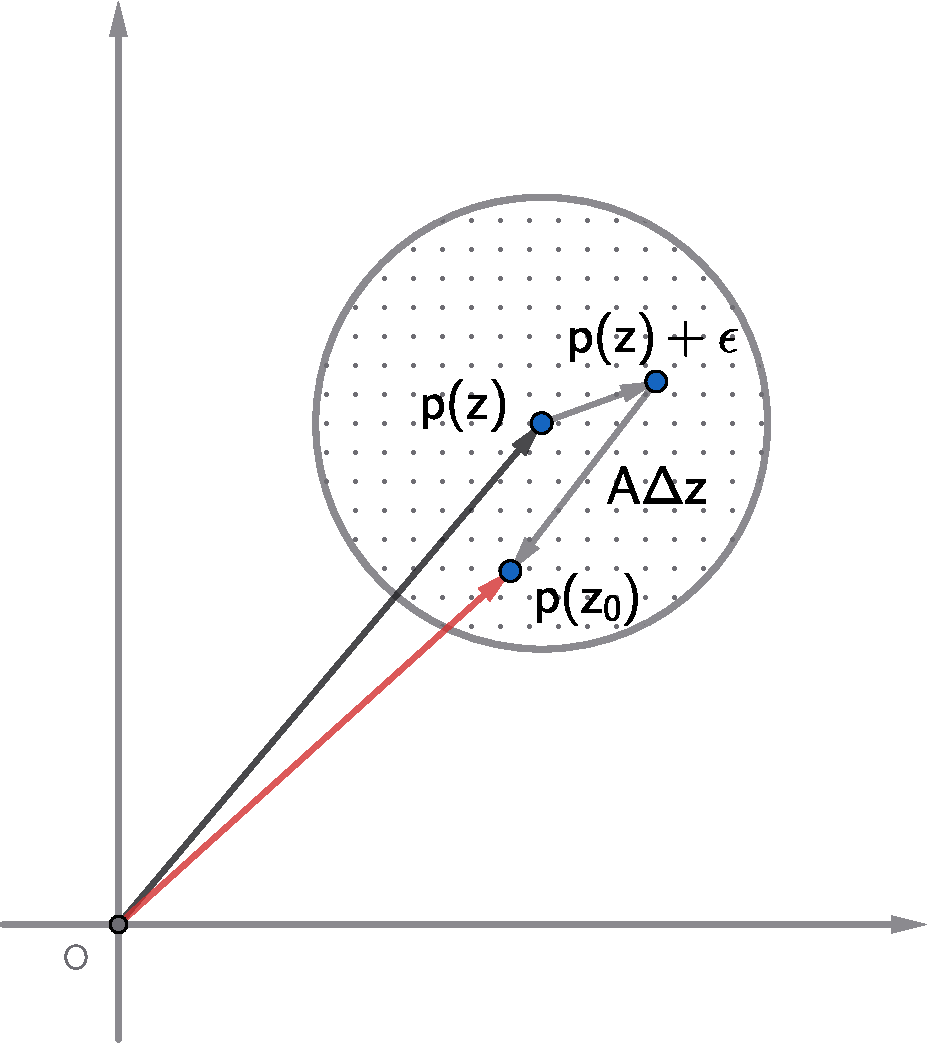
\includegraphics[scale=0.33]{img/dalambert-lemma}
  \caption{Find $p(z_0 + \Delta z)$ to be smaller than $p(z_0)$ by choosing $\Delta z$ appropriately.}
 \label{fig:dalambert-lemma}
\end{figure}

\begin{proof}
Let the polynomial be $p(z) = a_nz^n + \dotsb + a_1z + a_0$. The value of the polynomial at the complex number $z_0$ is $p(z_0)$, which is a vector with length $|p(z_0)|$. Argand aimed to find a complex number $z_0' = z_0 + \Delta z$ in the neighborhood of $z_0$ such that the value of the polynomial becomes:

\begin{align*}
p(z_0 + \Delta z) &= a_n (z_0 + \Delta z)^n + \dotsb + a_1 (z_0 + \Delta z) + a_0  \\
 & \text{binomial expand each one and collect terms} \\
 &= (a_n z_0^n + \dotsb + a_1 z_0 + a_0) + A_1 \Delta z + A_2 (\Delta z)^2 + \dotsb + A_n (\Delta z)^n \\
 &= p(z_0) + A \Delta z + \epsilon
\end{align*}

As $p(z)$ is not a constant, not all of $A_1, A_2, \dots A_n$ are zero. We find the first non-zero $A_i$, and define $A = A_i (\Delta z)^{i - 1}$, collecting the remaining terms into $\epsilon$. Since $\epsilon$ contains higher-order terms in $(\Delta z)^m$, when $|\Delta z|$ is small enough, we have $|\epsilon| < |A \Delta z|$. Next, Argand chooses a $\Delta z$ such that the vector $A \Delta z$ points in the opposite direction to $p(z_0)$, effectively canceling it out. This is shown in \cref{fig:dalambert-lemma}. Therefore, $|p(z_0 + \Delta z)| < |p(z_0)|$.
\end{proof}

However, Argand's proof of the fundamental theorem of algebra still has a flaw: it relies on the Extreme Value Theorem, which states that the modulus of a complex polynomial attains a minimum value. Argand considered this to be naturally true (treating it as an axiom), but this theorem was later first proven by Bolzano in 1830 for real numbers, and in 1874, Weierstrass proved that it also holds for complex numbers:

\index{extreme value theorem}
\begin{theorem}[Extreme Value Theorem]
A continuous function on a bounded closed set attains its maximum and minimum values.
\end{theorem}

With d'Alembert's lemma and the Extreme Value Theorem, we are going to reconstruct Argand's proof.

\begin{proof}
For any complex polynomial $p(z)$, consider the continuous function $|p(z)|$. When $|z|$ is large, $p(z) \approx a_n z^n$, and the leading term dominates the function value. As $|z|$ increases, the continuous function value $|p(z)|$ will exceed a sufficiently large circle $|z| = R$. Noting that $|z| \leq R$ is a bounded closed set, according to the Extreme Value Theorem, $|p(z)|$ attains its minimum value within it. By the definition of the modulus of a complex number (the length of a vector), this minimum value is $\geq 0$. But if the minimum value is $> 0$, it would contradict d'Alembert's lemma: we can always find a nearby point with a smaller modulus, thus smaller than the minimum value. Therefore, the minimum value can only be 0, which means there exists some $z_0$ such that $|p(z_0)| = 0$, so $p(z_0) = 0$.
\end{proof}

It proves the foundamental theorem of algebra, that is, any polynomial equation has at least one complex root. At this point, some friends may be eager to try solving quartic equations, quintic equations, or even higher degree equations by themselves. Hold on! There are indeed formulas for solving quartic equations, but there is \underdot{generally} no formula for solving equations of degree 5 or higher. Their solutions do exist, but they cannot be expressed using the operations of addition, subtraction, multiplication, division, and taking roots of the coefficients. After Cardano and Ferrari, it took mathematicians 300 years to finally uncover this secret. Italian mathematician Ruffini and Norwegian mathematician Abel successively proved this conclusion\footnote{Ruffini's proof in 1799 had flaws, and Abel first rigorously proved this conclusion in 1823. This theorem is now called the Abel-Ruffini theorem.}. Note that the term \enquote{generally} refers to equations of the form $ax^5 + bx^4 + cx^3 + dx^2 + ex + f = 0$. Special quintic equations do have formula solutions, such as $x^5 - 1 = 0$, and we can even find the method for ruler-and-compass construction of a regular pentagon by solving this equation (see \cref{sec:pentagon-equation}). The problem of which equations are solvable by radicals was completely solved by French mathematician Galois. This theory is called Galois theory.

\begin{figure}[htbp]
  \centering
  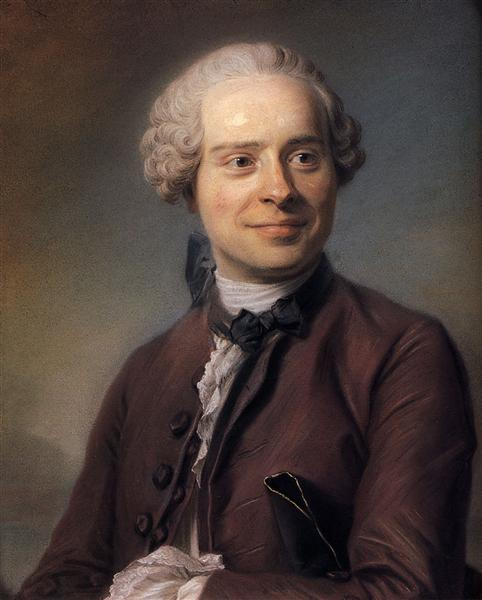
\includegraphics[scale=0.33]{img/d-alembert}
  \caption{Portrait of d'Alembert by Maurice Quentin de La Tour in 1753, housed in the Louvre Museum.}
 \label{fig:dalembert}
\end{figure}

\index{d'Alembert}
\begin{mdframed}
Jean Le Rond d'Alembert (1717–1783) was a famous French mathematician, physicist, and astronomer. He was an abandoned illegitimate child. This background influenced his entire life. d'Alembert's father was a military officer in the artillery, and his mother was a famous salon hostess in Paris. d'Alembert was one of the many romantic affairs of this socialite, but he was abandoned by his mother at birth on the steps of the Saint-Leu-Saint-Gilles church in Paris. He was thus named Jean Le Rond (after the place where he was found). A kind-hearted glassmaker couple took in the poor child, and d'Alembert regarded his foster mother always his mother in his own eyes.

d'Alembert's father later returned to Paris and secretly funded his education. However, when d'Alembert was 9 years old in 1726, his father died. He was sent to a Jansenist school. At the time of enrollment, his surname was Daremberg, but he soon changed it to Jean d'Alembert. The Jansenist school mainly trained theologians to promote doctrine, but d'Alembert was only interested in mathematics and disliked theology. He learnt about Descartes's physical ideas, which were eye-opening but not impressive to him. After graduating in 1735, d'Alembert decided to study law. He obtained a lawyer's certificate in 1738 but then switched to studying medicine. However, d'Alembert soon changed his mind again; he felt that medicine was not as good as theology, and his true love was still mathematics. d'Alembert was basically self-taught in mathematics and never stopped learning it, even during the preparation for the lawyer's exam.

The long experience of self-study both cultivated d'Alembert's outstanding independent thinking ability and creativity, but also limited him. He constantly proposed new ideas and explored new directions throughout his life, but he was not good at pushing them forward and clearly articulating them, and was soon surpassed by others. The supporters of these new ideas eventually became d'Alembert's competitors. This led to constant quarrels with other mathematicians, and complaints about others plagiarizing his work. Nevertheless, d'Alembert made very outstanding contributions in mathematics, physics, and astronomy. In 1739, at the age of 22, d'Alembert made a brief appearance at the Paris Academy of Sciences, and in 1741 he became a full member of the Academy. In 1743, he published the work \emph{Dynamics}, which included a new formulation of Newton's laws of motion and proposed the principle now named after him - the \enquote{d'Alembert's principle}. This principle allows us to transform dynamics problems into statics problems for analysis, laying the foundation for the creation of analytical mechanics. The following year, he successfully applied this principle to study fluid statics and dynamics, thus opening up the branch of mathematics called partial differential equations. This earned him the Berlin Academy of Sciences Prize in 1747. d'Alembert then applied partial differential equations to string vibrations and first gave the wave equation. This work attracted the attention and support of Euler. Euler quickly started research on partial differential equations, surpassing d'Alembert and achieving great results. Their relationship gradually deteriorated, and d'Alembert was indignant, believing that Euler had stolen his ideas. But d'Alembert's original text was chaotic and difficult to understand, so Euler simply started from scratch and derived richer results. d'Alembert strictly treated the concept of limits, being one of the few mathematicians at the time to view differentiation as a limit of functions, and distinguished between convergent and divergent series. He also proposed a method for determining the absolute convergence of series - the d'Alembert's ratio test. Additionally, d'Alembert also conducted research on the properties of complex numbers, probability theory,and other areas, and proved the fundamental theorem of algebra very early on. In 1764, Prussian King Frederick II wanted to appoint d'Alembert as the director of the Berlin Academy of Sciences, but he refused. Russian Empress Catherine II invited d'Alembert to tutor Grand Duke Paul, but he also refused.

d'Alembert lived during the Enlightenment, a time of great intellectual upheaval. The ideas of Diderot, Voltaire, and Rousseau were challenging the old religious views. d'Alembert also threw himself into this sweeping change. At Diderot's invitation, d'Alembert participated in the writing of the French \emph{Encyclopédie}. Although his contract only required him to be responsible for mathematics and astronomy, d'Alembert enthusiastically wrote on a wide range of topics, including philosophy, literature, and music. The latter half of d'Alembert's life was basically devoted to writing the encyclopedia and engaging in social activities, effectively ending his mathematical research. In 1772, he was elected as the perpetual secretary of the French Academy of Sciences. However, he was filled with regret that his declining energy prevented him from engaging in mathematical research. In 1777, he wrote to Lagrange\cite{MacTour-dAlembert} \enquote{What annoys me the most is the fact that geometry, which is the only occupation that truly interests me, is the one thing that I cannot do. All that I do in literature, although very well received in our public sessions of the French Academy, is for me only a way to fill the time for lack of anything better to do.}

The illegitimate child, the foster family, and the constant changes in his educational path, all contributed to d'Alembert's unique personality. d'Alembert was unmarried throughout his life. He met and fell in love with Julie de Lespinasse (1732–1776), the hostess of a famous salon in Paris. d'Alembert had a good relationship with his foster parents, and it was not until 1765, when he was 47 years old, that he left his foster parents due to illness and moved into Lespinasse's house. After Miss Lespinasse passed away in 1776, d'Alembert discovered that she still passionately loved other men. He was heartbroken and moved to the Academy of Sciences' apartment in the Louvre\cite{Ronald-2024}. d'Alembert died in Paris in 1783. Despite graduating from a church school and publicly believing in the existence of God in his writings, d'Alembert turned to a materialistic view under the influence of Diderot. Due to his opposition to religion during his lifetime, the Paris city government refused to hold a funeral for him. This great scientific giant left the world alone.
\end{mdframed}

\index{pure algebraic definition of complex numbers}
The geometric interpretation of complex numbers provides an intuitive explanation and gives them a legitimate status. However, some mathematicians insisted that numbers, as the epitome of mathematical abstraction, have meaning in their form alone. Remind that how Van der Waerden formalized negative numbers using pairs of numbers in \cref{sec:z-as-pair}. William Hamilton similarly formalized complex numbers using pairs of numbers. In 1831, Hamilton defined complex numbers as ordered pairs of values $(a, b)$ with the following rules for operations:

\begin{itemize}
\item addition of complex numbers: $(a, b) + (c, d) = (a + c, b + d)$
\item multiplication of complex numbers: $(a, b) (c, d) = (ac - bd, bc + ad)$
\end{itemize}

This definition is free from the \enquote{infamous} $\sqrt{-1}$, which was considered a symbol of the mysterious and controversial nature of complex numbers. In this definition, we can represent ordinary real numbers as pairs of the form $(a, 0)$, for example, $-1$ is represented as $(-1, 0)$. The imaginary unit $i$ is represented as $(0, 1)$, and we can verify that $i^2 = -1$:

\[(0, 1)(0, 1) = (0 \times 1 - 1 \times 1, 1 \times 0 + 0 \times 1) = (-1, 0)\]

\Cref{qn:pair-arithmetic-rules} asks to verify that the five arithmetic laws (commutative, associative, and distributive laws for addition and multiplication) hold for complex numbers defined in this way. This definition explicitly emphasizes that complex numbers, symbolized with $\mathbb{C}$, are compound. The real part of a complex number $z$ is denoted as $Re(z)$, which is the first two letters of Real; the imaginary part is denoted as $Im(z)$, which is the first two letters of Imaginary.

%% Biography of Hamilton

\section{A story of \textit{e}}

\index{compound interest} \index{Jacob Bernoulli}
Argand diagram beautifully connects complex numbers, geometry, and trigonometry, but this is not enough to show how magical complex numbers are. The real magic of complex numbers comes from another mystical constant $e$. However, unlike $\pi$, which was discovered by various civilizations in ancient times, $e$ was hidden behind nature, governing the reproduction of life, the accumulation of wealth, the passage of time... It wasn't until the development of calculus that people finally recognized the true nature of $e$. In 1683, Swiss mathematician Jacob Bernoulli (1655–1705) pondered the problem of financial \enquote{compound interest}, which was commonly found in scary usury. For example, suppose Antonio borrowed 100 ducats\footnote{Antonio and Shylock were characters in Shakespeare's \emph{The Merchant of Venice}, and ducat was the gold coin unit in Venice at that time.} from Shylock with a monthly interest rate of 5\%. After one month, Antonio had to repay $100 \times (1 + 5\%) = 105$ ducats. If Antonio failed to repay, after two months, he would owe $100 \times (1 + 5\%) \times (1 + 5\%) = 100 \times (1 + 5\%)^2 = 110.25$ ducats. Note that the interest from the first month was added to the principal to calculate the amount owed for the second month. Compound interest grows exponentially. If Antonio borrowed for a year, he would owe $100 \times (1 + 5\%)^{12} = 179.59 \approx 180$ ducats; if for two years, he would owe $322.5$ ducats in debt, more than three times the original principal. While Jacob Bernoulli's problem was about savings: if one deposits 100 ducats in a bank with an annual interest rate of 100\%, then at the end of the year, he will have $200$ ducats including principal and interest. If withdraws all the principal and interest every 6 months and then deposits it again, assuming the bank continuously calculates interest, the interest for 6 months is less than 100\%, only 50\%. But since interest is calculated twice by the end of the year, the total amount will be $100 \times (1 + \frac{1}{2} \times 100\%)^2 = 225$ ducats. This way one can get more than withdrawing all the money at the end of the year. If withdraws all the money every quarter and deposits it again, then interest is calculated 4 times, each time at $25\%$, and one will get $100 \times (1 + \frac{1}{4} \times 100\%)^4 \approx 244.14$ ducats at the end of the year. If withdraws and deposits every month, one will get $100 \times (1 + \frac{1}{12} \times 100\%)^{12} \approx 261.3$ ducats at the end of the year. Based on this, dividing the amount obtained at the end of the year by the principal of 100 ducats, we can derive the relationship between the actual annualized interest rate\footnote{In banking, the annual percentage rate (APR) and the actual annualized interest rate (Internal Rate of Return, IRR) are different concepts. The former is calculated using simple interest, while the latter is calculated using compound interest.} and the number of times $n$ of withdrawing and depositing:

\be
(1 + \frac{1}{n})^n
\ee

Jacob Bernoulli discovered that although increasing the frequency of withdrawing and depositing (the number of times $n$) increases the amount of money, it does not increase indefinitely. The rate of increase slows down and gradually approaches a constant value, as shown in \cref{tab:compound-interest}. He then defined a constant, which is the limit as $n$ approaches infinity:

\begin{table}[ht]
  \caption{Actual annualized interest rate versus number of withdrawals and deposits}
  \centering
  \begin{tabular}{|l|l|l|}
    \hline
    cadence & $n$ & actual annualized interest rate \\
    \hline
    year & 1 & 2 \\
    half year & 2 & 2.25 \\
    quarter & 4 & 2.4414 \\
    month & 12 & 2.6130 \\
    day & 365 & 2.7146 \\
    hour & 8760 & 2.7181 \\
    \hline
  \end{tabular}
  \label{tab:compound-interest}
\end{table}

\index{e} \index{definition of e as a limit}
\be
e = \lim_{n \to \infty} (1 + \frac{1}{n})^n
\ee

This is the constant $e$ defined in high school mathematics classes. It is the first constant in the history of mathematics to be defined using limits. However, Jacob Bernoulli neither named this constant nor patiently calculated its value. He only estimated the range of this constant using the binomial theorem\cite{MacTour-e}:

\begin{proposition}[Jacob Bernoulli]
The range of the constant $e$ is: $2 < e < 3$
\end{proposition}

\begin{proof}
\begin{align*}
e &= \lim_{n \to \infty} (1 + \frac{1}{n})^n \\
  &= 1 + \binom{n}{1}\frac{1}{n} + \binom{n}{2}\frac{1}{n^2} + \dotsb && \text{binomial expansion} \\
  &= 1 + \cancel{n}\frac{1}{\cancel{n}} + \frac{n(n-1)}{2!n^2} + \frac{n(n-1)(n-2)}{3!n^3} + \dotsb \\
  &> 1 + 1 = 2
\end{align*}

On the other hand,
\begin{align*}
e &= 2 + \frac{1}{2!}\frac{n-1}{n} + \frac{1}{3!}\frac{n-1}{n}\frac{n-2}{n} + \dotsb \\
  &\leq 2 + \frac{1}{2} + \frac{1}{2 \cdot 3} + \frac{1}{2 \cdot 3 \cdot 4} + \dotsb && \text{every }\frac{n-k}{n} < 1 \\
  &< 2 + \frac{1}{2} + \frac{1}{2 \cdot 2} + \frac{1}{2 \cdot 2 \cdot 2} + \dotsb && \text{scaling} \\
  &= 2 + (\frac{1}{2} + \frac{1}{2^2} + \frac{1}{2^3} + \dotsb) \\
  &= 2 + 1 = 3 && \text{sum of geometric sereies} \qedhere
\end{align*}
\end{proof}

\index{Johann Bernoulli}
$e$ is well known as the base of the natural logarithm, how does it connected with compound interest? Jacob's brother Johann Bernoulli studied the properties of exponentials. Before that, people only considered logarithms as pure numbers, not as functions, and even printed long logarithm tables for convenient calculations. Johann Bernoulli connected logarithms and exponentials from the perspective of functions:

\index{exponential functions} \index{logarithmic functions}
\begin{align*}
  y = a^x && x = \log_a y
\end{align*}

This is a pair of functions and their inverses. When $a = e$, it becomes:

\begin{align*}
  y = e^x && x = \ln y
\end{align*}

\begin{figure}[htbp]
 \centering
 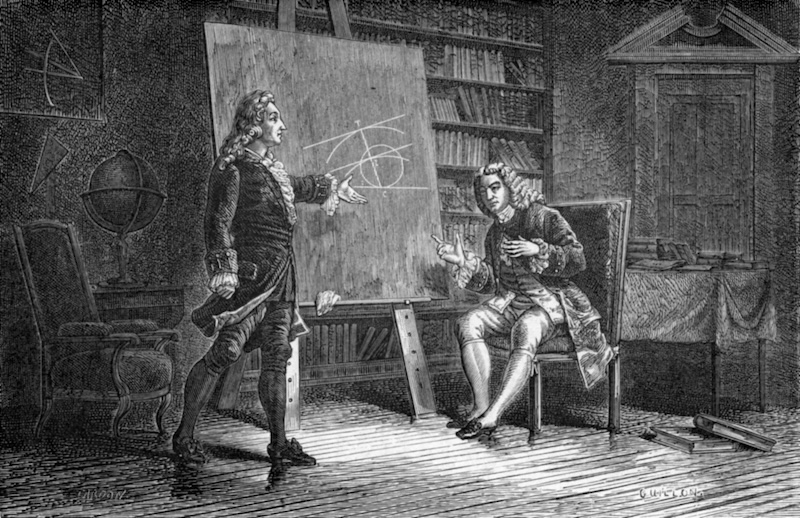
\includegraphics[scale=0.3]{img/Bernoulli-brothers}
 \caption{Bernoulli brothers, by Charles Joseph Traviers}
 %% （Charles Joseph Traviers）
 \label{fig:Bernoulli-brothers}
\end{figure}

\index{John Napier} \index{Logarithm}
It changes the starting point of the history of $e$ to 1618, when the Scottish mathematician John Napier invented logarithms (see \cref{fig:napier}) and printed the first logarithm tables. Coincidentally, the base of the earliest logarithm tables was not 10, but the natural logarithm $e$. Of course, Napier did not realize the existence of the constant $e$; he just wanted to solve the problem of complex multiplication calculations. At that time, astronomical observations and navigation often involved multiplication calculations with huge numbers. We now know that when calculating $Z = XY$, if we let $X = a^x$ and $Y = a^y$, then $Z = a^{x + y}$. So we only need to look up the logarithms $x$ and $y$ corresponding to $X$ and $Y$ in the logarithm tables, add them together to get $z = x + y$, and then look up the number $Z$ corresponding to the logarithm $z$ in the tables. Later, English mathematician Henry Briggs reminded Napier that it would be more convenient and practical to use logarithms with base 10. But by then, Napier was already old and unable to undertake the huge calculations to make this change. The selfless Briggs took it upon himself to create logarithm tables with base 10 and published them in Napier's name\cite{Amerson-2021}.

\index{Mercator map}
Logorithm is a revolutionary invention in terms of computational efficiency, and it is a product of the Age of Exploration. You must have seen world maps printed on paper. Mapping the spherical surface of the Earth onto a rectangular piece of paper without distortion is a difficult problem, and mathematically, it is unsolvable. The world map we commonly see is called the \enquote{Mercator map,} named after the geographer Gerardus Mercator (1512–1594), a cartographer and geographer from Flanders (now Belgium). The Mercator projection imagines rolling a rectangular piece of paper into a cylinder, then placing a transparent globe inside this cylinder so that the equator just touches the cylindrical surface (see \cref{fig:mercator}). At this point, if we place a lamp at the center of the globe, the shadow of the globe will appear on the paper. By tracing this shadow with a pen and then unrolling the paper, we get the Mercator map. The Mercator map preserves directions and shapes well, but areas and distances become increasingly distorted as you move closer to the poles.

\begin{figure}[htbp]
 \centering
 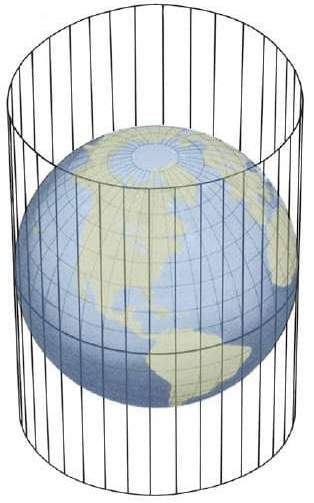
\includegraphics[scale=0.3]{img/mercator-map}
 \caption{Mercator map}
 \label{fig:mercator}
\end{figure}

\index{Naturual logarithm}
There was another Mercator, the mathematician Nicolaus Mercator (1620–1687), whose original name was Niklaus Kauffman, and later changed his family name to Mercator. It was a common thing to do at that time. Mercator was the Latin form of \enquote{merchant}. In 1668, Nicolaus Mercator published a book about logarithms, in which he named the logarithm with base $e$ as the \enquote{natural logarithm}. Although this work came after Jacob Bernoulli's discovery of $e$, Mercator was unaware of the existence of $e$. We have to wait for Euler to name this constant.

\subsection{The most beatiful formula}
Leonhard Euler was a student of Johann Bernoulli. When he was thinking along the direction of exponential v.s. logarithmics, he discovered a surprising and beautiful result: the derivative of $e^x$ is itself.

\be
(e^x)' = e^x
\ee

We shall use the modern language and notation of limits in below proof which was not available to Euler at his time.

\begin{proof}
By the definition of deriative:

\be \label{eq:derive-of-e}
(e^x)' = \lim_{\Delta x \to 0} \frac{e^{x + \Delta x} - e^x}{\Delta x} = \lim_{\Delta x \to 0} \frac{e^xe^{\Delta x} - e^x}{\Delta x} = e^x\lim_{\Delta x \to 0} \frac{e^{\Delta x} - 1}{\Delta x}
\ee

In Jacob Bernoulli's definition of $e$, taking the reciprocal of $n$, we let $t = \frac{1}{n}$, we get:

\be \label{eq:def2-of-e}
e = \lim_{n \to \infty} (1 + \frac{1}{n})^n = \lim_{t \to 0} (1 + t)^{\frac{1}{t}}
\ee

Let $u = e^{\Delta x} - 1$, then using the inverse relationship between logarithmic and exponential functions pointed out by Johann Bernoulli: $\Delta x = \ln (1 + u)$. Substituting into the above limit:

\begin{align*}
\lim_{\Delta x \to 0} \frac{e^{\Delta x} - 1}{\Delta x} &= \lim_{u \to 0} \frac{u}{\ln (1 + u)} = \lim_{u \to 0} \frac{1}{\frac{1}{u}\ln (1 + u)} && \text{by } b \ln a = \ln a^b \\
  &= \lim_{u \to 0} \frac{1}{\ln (1 + u)^{\frac{1}{u}}} && \text{by \cref{eq:def2-of-e}} \\
  &= \lim_{u \to 0} \frac{1}{\ln e} = 1 && \text{by } \ln e = 1
\end{align*}
Substituting this result back into \cref{eq:derive-of-e} proves that $(e^x)' = e^x$.
\end{proof}

It implies that the derivative of derivative of $e^x$ is also itself, because: $(e^x)'' = ((e^x)')' = (e^x)' = e^x$. No matter how many times we take the derivative of $e^x$, the result is always $e^x$. Substituting this result into the Maclaurin formula (see \cref{eq:maclaurin}) gives the famous series expansion:

\begin{align*}
e^x &= f(0) + \frac{f'(0)}{1!}x + \frac{f''(0)}{2!}x^2 + \dotsb + \frac{f^{(n)}(0)}{n!}x^n + \dotsb \\
  &= e^0 + \frac{e^0}{1!}x + \frac{e^{0}}{2!}x^2 + \dotsb + \frac{e^0}{n!}x^n + \dotsb && \text{by }f^{(n)}(x) = e^x \\
  &= 1 + \frac{x}{1!} + \frac{x^2}{2!} + \frac{x^3}{3!} + \dotsb
\end{align*}

\index{e as infinite series}
With the series expansion, Euler could do something that Jacob Bernoulli couldn't: find an approximation of $e$. Euler substituted $x = 1$ into the expansion to get the famous series definition of $e$:

\be
e = 1 + \frac{1}{1!} + \frac{1}{2!} + \frac{1}{3!} + \dotsb
\ee

Euler calculated the first 20 terms of the series and summed them up to get an approximation of $e$ with 18 decimal places: $e = 2.718281828459045235$. Euler achieved this in 1731 at the age of 24. He was so excited that he wrote a letter to his good friend Goldbach to share these results. In the letter, he gave this constant a name: \enquote{$e$.} Many people thought it was the first letter of Euler's name, and some said it was the first letter of \enquote{exponential,} but actually neither is true. Euler had a habit of using vowel letters a, e, i, o, u to name constants, and coincidentally, a had already been used before, so Euler used the second vowel letter e.

%% e isn't called Euler's constant. Euler's constant is \gamma in the sum of harmonic series:
%% \( \sum_{n \leq x} \frac{1}{n} = \ln x + \gamma + O(\frac{1}{x}) \)

Euler clearly stated in his letter to Goldbach that $e$ was the value of $(1 + \frac{1}{n})^n$ when $n$ approaching infinity, and it was equal to 1 plus the reciprocals of all factorials. He continued his research and published even more magical and beautiful results in 1748. Euler separated the odd and even terms in the series expansion of $e^x$ and connected them to the famous series expansions of trigonometric functions:

\begin{align*}
\sin x &= x - \frac{x^3}{3!} + \frac{x^5}{5!} - \frac{x^7}{7!} + \dotsb \\
\cos x &= 1 - \frac{x^2}{2!} + \frac{x^4}{4!} - \frac{x^6}{6!} + \dotsb
\end{align*}

Euler discovered the relationship between complex numbers and $e$ by substituting the variable $ix$ into the series expansion of $e^x$.

\begin{align*}
e^{ix} &= 1 + (ix) + \frac{(ix)^2}{2!} + \frac{(ix)^3}{3!} + \frac{(ix)^4}{4!} + \dotsb \\
  &= 1 + ix - \frac{x^2}{2!} - i\frac{x^3}{3!} + \frac{x^4}{4!} + \dotsb && i^2 = -1\\
  &= (1 - \frac{x^2}{2!} + \frac{x^4}{4!} - \frac{x^6}{6!} + \dotsb) + i(x - \frac{x^3}{3!} + \frac{x^5}{5!} - \frac{x^7}{7!} + \dotsb ) \\
  &= \cos x + i\sin x
\end{align*}

\index{Euler formula}
This is the formula $e^{i\theta} = \cos \theta + i\sin \theta$ that we learned in high school mathematics classes. The geometric meaning of the right side is very clear: it is a complex number on the Argand diagram with modulus 1 and argument $\theta$. This gives a geometric meaning to $re^{i\theta}$, which is a complex number with modulus $r$ and argument $\theta$. Further combining with De Moivre's formula (see \cref{eq:de-Moivre}), we get:

\[
e^{in\theta} = \cos n\theta + i\sin n\theta = (\cos \theta + i\sin \theta)^n = (e^{i\theta})^n
\]

This means that the $n$-th power of a vector on the unit circle with argument $\theta$ is equivalent to rotating the vector by an angle of $n\theta$. Euler substituted the special value $\theta = \pi$ into this formula and obtained a beatiful identity:

\be \label{eq:euler}
e^{i\pi} = \cos \pi + i\sin \pi = -1
\ee

This special case, $e^{i\pi} + 1 = 0$ is called Euler's identity. Many people consider it the most beautiful formula in the universe, as it magically connects two famous irrational numbers $e$ and $\pi$, the imaginary unit $i$, the additive identity 0, and the multiplicative identity 1 together.

\begin{figure}[htbp]
  \centering
  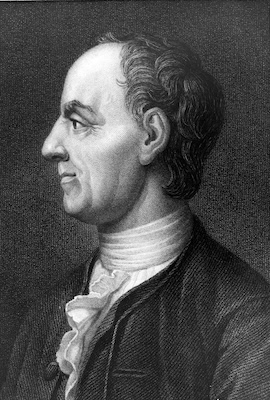
\includegraphics[scale=0.45]{img/Euler}
  \caption{Leonhard Euler, by Johann Georg Brucker}
 \label{fig:Euler}
\end{figure}

\index{Euler}
\begin{mdframed}
Below biography of Leonhard Euler is adapted from André Weil's classic book, \emph{Number Theory: An approach through history From Hammurapi to Legendre}.

In 1707, when Euler was born, Jacob Bernoulli was dead, and Johann had succeeded him; Euler's father, Paul Euler, was a parish priest established in Riehen near Basel. He had studied theology at the university of Basel, while at the same time attending the lectures of Jacob Bernoulli; he had planned a similar career for his son. Young Leonhard entered the theological school of the University of Basel at the age of 13, studying in philosophy and law, but soon showed his talent in mathematics. He studied mathematics with Johann Bernoulli every Saturday afternoon. Johann's two sons Nicolas and Daniel. Euler became their close friend and Johann's favorite disciple; in his old age, he liked to recall how he had visited his teacher every Saturday and laid before him the difficulties he had encountered during the week, and how hard he had worked so as not to bother him with unnecessary questions.

Three monarchs came to play a decisive role in Euler's career: Peter the Great, Frederic the Great, and the Great Catherine. Peter died in 1725; but he had had time to found Saint Petersburg and made plans for an Academy of Sciences modelled on what he had seen in the West; those plans were faithfully carried out by his widow. In 1725 the two younger Bernoullis, Nicolas and Daniel, were called there. Nicolas died the next year, apparently of appendicitis. About the same time an offer went to Euler to join the Petersburg Academy. He was not quite twenty years old; he had just won a prize for an essay on ship-building, never having seen a sea-going ship in his life. He had no early prospects at home. He accepted with alacrity.

From Base1 he sailed down the Rhine to Mainz, then traveled to Lübeck, mostly on foot, visiting Christian Wolff on the way; this was a philosopher and follower of Leibniz, banished from Berlin (as he told Euler) by a king with little understanding for philosophy; his hobby-horse was Leibniz's theory of monads, and Euler was clearly not impressed. From Lübeck a ship took the young mathematician to Petersburg.

Following Peter the Great's plan, Saint Petersburg Academy was well-endowed and provided with ample funds and good libraries. Their members enjoyed considerable freedom; their primary duty was to contribute substantially to the academy's publications and keep high its prestige in the international scientific world. At the same time they were the scientific advisers to the monarch and to state authorities. Although some of these duties were not always welcome, Euler fully understood that the state was paying for the academy. In 1727, however, the political situation had changed by the time Euler reached Petersburg. Under a new czar all academic appointments were in abeyance. On the strength of his prize essay, Euler was commissioned into the Russian navy, but not for long. Soon he was a salaried member of the academy, at first with the junior rank of \enquote{adjunct.} When his friend Daniel left for Basel in 1733, he was appointed in his place; thus he could afford to marry, naturally into the local Swiss colony, and to buy for himself a comfortable house. His bride was the daughter of the painter Gsell; in due course she was to give birth to thirteen children, out of whom only three sons survived. The eldest son Johann Albert, born in 1734, was to become one of his father's collaborators, and later a leading member of the academy. During his fourteen years in Petersburg, Euler did a great deal of outstanding work in analysis, number theory, and mechanics.

Once Euler was thus well established in Petersburg, his productivity exceeded all expectations, in spite of the comparative isolation in which he had been left by Daniel Bernoulli's departure. It was hardly interrupted by a severe illness in 1735 and the subsequent loss of his right eye. This is the reason that most portraits of Euler are either from left side (for example, \cref{fig:Euler}) or have his right eye obscured by shadow. He had beyond doubt become the most valuable member of the Academy, and his reputation had been growing by leaps and bounds, when two events in the higher spheres of European politics brought about a major change in his peaceful life. In Petersburg the death of the czarina in 1740, a regency, and the ensuing turmoils, seemed to threaten the very existence of the Academy. Just at this juncture Frederic II succeeded his father (the same king who had so cavalierly thrown Chr. Wolff out of Berlin) on the throne of Prussia; he immediately took steps directed towards the establishment of an academy under his patronage, for which he sought out the most famous names in European science; naturally Euler was on the list. A munificent offer from Frederic, coupled with a fast deteriorating situation in Petersburg, brought Euler to Berlin in July 1741, after a sea-voyage of three weeks on the Baltic during which he alone among his family (or so he claimed) had been free from sea-sickness. Euler was to spend the next 25 years in Berlin, where his work was even more varied than in Petersburg, and where his research in planetary motion, rigid body motion, thermodynamics, ballistics, and demography was closely connected with his mathematical investigations. His work on differential equations, on the differential geometry of surfaces, and in other fields of mathematics during this period was groundbreaking.

With Euler's change of residence one might have expected that the steady flow of his publications would be diverted from Petersburg to Berlin; but far from it! He was not only allowed to keep his membership in the Petersburg Academy, but his pension from Petersburg was continued, and he was intent upon giving his former colleagues value for their money. Well might his great-grandson P.-H. Fuss describe Euler's Berlin period as \enquote{twenty-five years of prodigious activity.} More than 100 memoirs sent to Petersburg, 127 published in Berlin on all possible topics in pure and applied mathematics were the products of those years, side by side with major treatises on analysis, but also on artillery, ship-building, lunar theory; not to mention the prize-winning essays sent to the Paris academy. As years went by, Euler and Frederic became disenchanted with each other. The king was not unaware of the lustre that Euler was throwing upon his academy, but French literati stood far higher in his favor. He was seeking to attract d'Alembert to Berlin and was expected to put him above Euler as head of the Academy. Euler was spared this blow to his self-esteem; d'Alembert, forewarned perhaps by Voltaire's unpleasant experience with Frederic in 1753, enjoyed basking in the king's favor for the time of a short visit but valued his freedom far too highly to alienate it more durably. Nevertheless, as early as 1763, Euler's thoughts started turning again towards Russia.

Fortunately another political upheaval had just taken place there. In 1762 the czar's German wife had seized power as Catherine II after ridding herself and Russia of her husband. One of her first projects was to restore the Petersburg academy to its former glory. This was almost synonymous with bringing Euler back. Negotiations dragged on for three years. Finally, in 1766, the Russian ambassador in Berlin was instructed to request Euler to write his own contract. Frederic, realizing too late the magnitude of this loss, had tried to put obstacles in the way; he soon found that he could not afford to displease the imperial lady. In the same year Euler was back in Petersburg, after a triumphal journey through Poland where Catherine's former lover, king Stanislas, treated him almost like a fellow-sovereign. By then Euler was losing his eyesight. In 1770, in answer to a letter from Lagrange, he wrote he could not read, but that he had someone read to him and that he could verify the results by mental calculation. An operation was attempted in 1771 and was successful at first, but the eye soon became infected, and total or near-total blindness ensued\cite{Weil-1983}. Just as deafness did not stop Beethoven's musical creativity, blindness did not stop Euler's mathematical exploration\cite{HanXueTao2009}. With the help of a secretary, Euler actually became more productive in his research in various fields. In 1775, he completed an average of one mathematical paper per week. Half of Euler's works were actually completed after he became completely blind.

Euler's extraordinary knowledge, inexhaustible creative energy, and unprecedentedly rich body of work are all astonishing. He started publishing papers at the age of 19 and wrote a vast number of books and papers for more than half a century until he was 76 years old. Euler's name can be found in almost every field of mathematics. He is the most prolific mathematician in the history of science, with a total of 856 papers and 31 monographs published in his lifetime. This does not even include the portion lost in the fire of Saint Petersburg in 1771. This record was not broken until the 20th century by Hungarian mathematician Paul Erdős (see \cref{sec:Erdos}). Euler's prolific output was not accidental; he had an amazing memory and could perform complex mental calculations. The French physicist Arago said, \enquote{Euler calculates as easily as breathing, or an eagle flying.} Euler could work in any unfavorable environment; he often completed papers with a child on his lap and did not care about the child making noise nearby.

Among the many remarkable aspects of Euler's work, one that stands out is his ability to write for different audiences. \emph{The Letters to a German Princess} is one of the most successful popular books on science ever written, and the Elements of Algebra, which is still in print. Euler placed great emphasis on clear and understandable expression. Many of the mathematical symbols we are familiar with today were carefully chosen by Euler, such as $\pi$ (1736), the imaginary unit $i$ (1777), $e$ (1748), the trigonometric functions $\sin$ and $\cos$ (1748), $tg$ (1753), $\Delta x$ (1755), the summation symbol $\sum$ (1755), and the function notation $f(x)$ (1734) \cite{HanXueTao2009}.

On 18 September 1783, Euler was having dinner with his friends. Uranus had just been discovered, and Euler listed the essentials for calculating the orbit of Uranus. After dinner, while drinking tea and playing with his granddaughter, his pipe suddenly fell from his hand. He said, \enquote{My pipe}, and bent down to pick it up, but never stood up again. He murmured, \enquote{I am dead...} and thus \enquote{stopped calculating and living} (French mathematician Condorcet's words).
\end{mdframed}

\subsection{Eadem mutata resurgo}

\index{Equiangular spiral} \index{Logarithmic spiral}
Despite not being able to see Euler's achievements, Jacob Bernoulli foresaw the birth of $e^x$ during his lifetime. In 1638, Descartes discovered a magical spiral called the \enquote{equiangular spiral}, also known as the \enquote{logarithmic spiral} (see \cref{fig:decartes-equiangular-spiral}).

\begin{figure}[htbp]
 \centering
 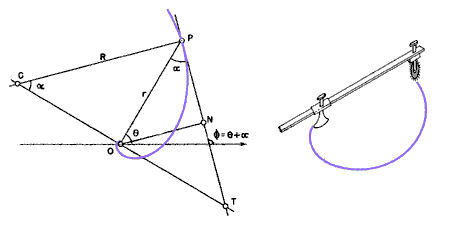
\includegraphics[scale=0.5]{img/descartesspiral}
 \caption{Descartes discovered the equiangular spiral in 1638.}
 \label{fig:decartes-equiangular-spiral}
\end{figure}

As the name suggests, Descartes found that the angle between the tangent line at any point on the spiral and the line connecting the point to the origin is constant, as shown in \cref{fig:equiangular} \cite{Descartes-1638}. Torricelli\footnote{Italian mathematician and physicist. He was the first to measure atmospheric pressure through experiments.} conducted independent research on the equiangular spiral and found that if we let $r$ be the distance from the origin $O$ to a point $P$ on the spiral, and $\theta$ be the angle between $OP$ and the horizontal axis, as shown on the left side of \cref{fig:decartes-equiangular-spiral}, then as $\theta$ increases, $r$ increases in a geometric progression (i.e., in a way of a geometric sequence). This definition is a typical polar coordinate definition. If we let a point on the curve be $(r, \theta)$, then Torricelli's definition is equivalent to:

\begin{figure}[htbp]
 \centering
 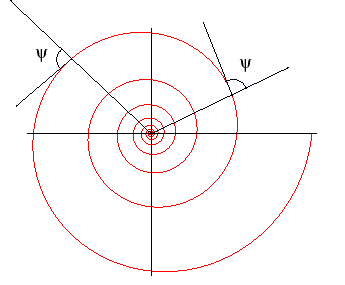
\includegraphics[scale=0.4]{img/equiangular}
 \caption{The meaning of \enquote{equiangular}}
 \label{fig:equiangular}
\end{figure}

\[
r = ka^\theta
\]

\index{Spiral mirabilis}
where $k$ and $a$ are constants. So when $\theta$ increases by a factor of 2, $r$ increases to $r^2$; when $\theta$ increases by a factor of 3, $r$ increases to $r^3$, and so on... \cref{qn:equiangular} requires proving that Torricelli's definition and Descartes's definition are equivalent. Jacob Bernoulli conducted in-depth research on this spiral and discovered many fascinating properties. The most astonishing is that no matter how you transform it, scale it, take its evolute, involute, or pedal curve, the result is always the same - the same shape of spiral. In 1692, he named this fascinating spiral the \enquote{spiral mirabilis} and decided to engrave this spiral on his tombstone after his death, as shown in \cref{fig:bernoulli-tomb} \cite{MacTour-Equiangular}. He left a famous Latin epitaph: Eadem mutata resurgo, which translates to \emph{Though changed, I shall arise the same} in English \cite{Maor-2010}. The content of the epitaph is:

\begin{figure}[htbp]
 \centering
 \subcaptionbox{Jacob Bernoulli's tomb stone. \label{fig:bernoulli-tomb}}{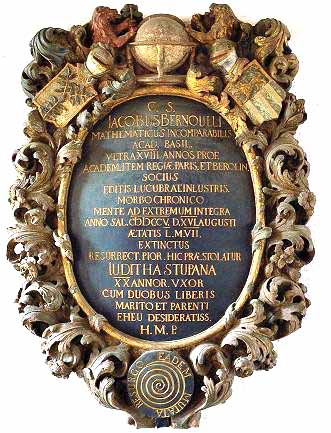
\includegraphics[scale=0.4]{img/bernoulli-tomb}}
 \subcaptionbox{The spiral on the tombstone\label{fig:bernoulli-epitaph}}{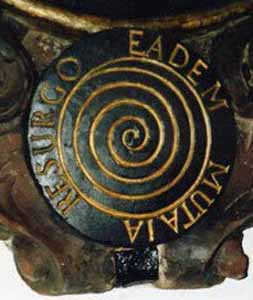
\includegraphics[scale=0.4]{img/bernoulli-epitaph}}
 \caption{Jacob Bernoulli's epitaph: Eadem mutata resurgo\cite{MacTour-Bernoulli-tomb}}
\end{figure}

\begin{mdframed}
\begin{verse}
Jacob Bernoulli \\
Incomparable mathematician \\
Professor at the University of Basel \\
For more than 18 years \\
Member of the Royal Academies of Paris and Berlin \\
Famous for his writings \\
Of a chronic illness, of sound mind to the end \\
Died in the year of grace 1705, the 16th of August \\
At the age of 50 years and 7 months \\
Awaiting the resurrection \\
Judith Stupanus \\
His wife for 20 years \\
And his two children \\
erected a monument to the husband and father \\
they miss so much.
\end{verse}
\end{mdframed}

\index{Achimedes spiral}
Unfortunately, the mason who did the carving misunderstood the instructions and gave him an Archimedean spiral instead, as shown in \cref{fig:bernoulli-epitaph}. What is the difference between these two spirals? The Archimedean spiral has equal spacing between each turn, while the equiangular spiral has spacing that follows a geometric progression (see \cref{fig:equiangular-spiral}). If we express them in polar coordinates, the equation of the Archimedean spiral is $r = a\theta$. When we rotate the Archimedean spiral at a constant speed, the intersection points with the coordinate axes will translate at a constant speed. So why is this spiral also called a \enquote{logarithmic spiral}? From the perspective of inverse functions:

\begin{figure}[htbp]
 \centering
  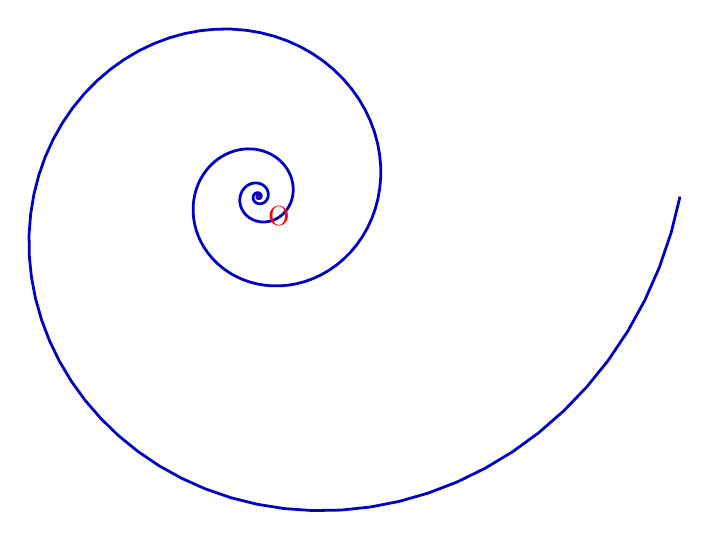
\begin{tikzpicture}[scale=0.1]
      % r = a*e^(b*θ)
      \def\a{0.1}
      \def\b{0.2}
      \def\turns{5}

      \draw[
          line width=1pt,
          blue!80!black,
          domain=0:{2*pi*\turns},  % domain of the angle
          samples=360,
          variable=\t
      ] plot (
          {exp(\b*\t)*\a*cos(\t r)},  % x coordinate
          {exp(\b*\t)*\a*sin(\t r)}   % y coordinate
      );

      % origin
      \fill[red] (0,0) circle (2pt) node[below right] {O};
  \end{tikzpicture}
  \caption{Equiangular spiral (logarithimc spiral)}
  \label{fig:equiangular-spiral}
\end{figure}

\begin{align*}
r = ka^\theta && \theta = \log_{a} \frac{r}{k}
\end{align*}

\index{change of base formula}
For any point on the spiral, the angle $\theta$ and the radius $r$ have a logarithmic relationship. Therefore, the French mathematician Pierre Varignon (1654–1722) named this spiral the \enquote{logarithmic spiral}. We have learned the change of base formula in high school: $\log_a x = \dfrac{\ln x}{\ln a}$ (see \cref{qn:change-base} for a proof of this formula), so:

\begin{align*}
\theta &= \log_a \frac{r}{k} = \frac{\ln \frac{r}{k}}{\ln a} && \text{change of base}\\
\ln \frac{r}{k} &= \theta(\ln a) && \text{mulitply both sides by }\ln a \\
\frac{r}{k} &= e^{\theta \ln a} = e^{b\theta} && \text{raise to power of }e\text{, let }b = \ln a \\
r &= k e^{b\theta}
\end{align*}

Thus, we have obtained the polar coordinate equation of the equiangular spiral with base $e$. This formula was beyond Jacob Bernoulli's imagination, but it can easily reveal why \enquote{Eadem mutata resurgo.}

\begin{proposition}[Jacob Bernoulli]
The shape of the equiangular spiral remains unchanged after scaling.
\end{proposition}

\begin{proof}
By the polar coordinate equation of equiangular spiral $r = ke^{b\theta}$, scaling the radius by a factor of $a$ gives:

\begin{align*}
r' &= (ak)e^{b\theta} = e^{\ln a} k e^{b\theta} \\
   &= ke^{b\theta}e^{\ln a} = k e^{b\theta + \ln a} \\
   &= ke^{b(\theta + \theta_0)} && \text{令} \theta_0 = \frac{\ln a}{b}
\end{align*}

It is equivalent to rotating the angle by $\theta_0$, and the shape of the spiral remains unchanged after rotation.
\end{proof}

\Cref{qn:exp-from-fixed-point} requires using the property of \enquote{Eadem mutata resurgo} to find the expansion of $e^x$. The equiangular spiral also has a connection with $e$ and complex numbers.

\begin{proposition}
For any complex number $z = a + bi$ with $b \ne 0$, the geometric sequence $z, z^2, z^3, \dotsc$ formed by its powers is distributed on an equiangular spiral.
\end{proposition}

\begin{proof}
Applying Euler's formula, we can express $z$ in the form of $z = c(\cos\theta_0 + i\sin\theta_0)$, where $c = \sqrt{a^2 + b^2}$ and $\theta_0 = \tan^{-1} \dfrac{b}{a}$. Since $b \ne 0$, we have $\theta_0 \ne 0$. Using De Moivre's formula, the $n$-th term of the geometric sequence is:

\[
z^n = c^n(\cos\theta_0 + i\sin\theta_0)^n = c^n(\cos n\theta + i\sin n\theta)
\]

We are going to represent $z^n$ in polar coordinates. Its argument is $\theta = n\theta_0$, and its modulus is:

\begin{align*}
r &= c^n = e^{\ln(c^n)} && \text{change base} \\
  &= e^{n\ln c} && \text{rule of logarithm} \\
  &= e^{\frac{\theta}{\theta_0}\ln c} = ke^{b\theta} && \text{where }k=1, b = \frac{\ln c}{\theta_0} \text{, form of equiangular spiral} \qedhere
\end{align*}
\end{proof}

It isn't by accident that the equiangular spiral arises everywhere. De Moivre used the method of equating coefficients to find the general term formula of the Fibonacci sequence, which satisfies the equation of the equiangular spiral when $n$ is large (see \cref{app:fibonacci-formula}). The growth of many creatuers and plants satisfy the Fibonacci formula, such as the growth of the nautilus shell (see \cref{fig:nautilus}), broccoli, and sunflower florets, thus presenting the shape of an equiangular spiral.

\begin{figure}[htbp]
 \centering
 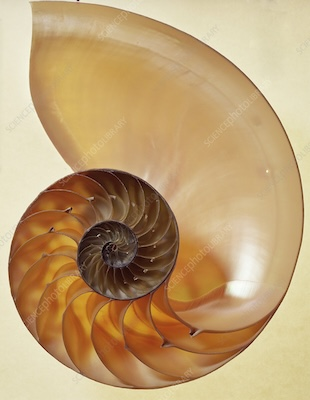
\includegraphics[scale=0.4]{img/nautilus}
 \caption{The growth of nautilus shell presents an equiangular spiral}
 \label{fig:nautilus}
\end{figure}

Complex numbers are quite different from the numbers we were familiar with before. Whether it's natural numbers, rational numbers, or irrational numbers, they all have a specific position on the number line. Complex numbers, however, jump out of the number line and come to the complex plane. The previous numbers were one-dimensional, with a definite size and a specific position on the number line. Complex numbers, on the other hand, are two-dimensional; whether represented by real and imaginary parts or by modulus and argument, it takes two quantities to determine a complex number. Two complex numbers usually cannot be compared in size; we can only compare their moduli. Despite being so peculiar, complex numbers can still be calculated with each other and with real numbers, and they satisfy the previously known arithmetic laws, including the commutative and associative properties of addition and multiplication, and the distributive property of multiplication over addition. The distance between two real numbers $a$ and $b$ on the number line is $|a - b|$, while the distance between two complex numbers $z_1 = x_1 + y_1i$ and $z_2 = x_2 + y_2i$ in the complex plane is $|z_1 - z_2|$. This is because:

\[
|z_1 - z_2| = |(x_1 - x_2) + (y_1 - y_2)i| = \sqrt{(x_1 - x_2)^2 + (y_1 - y_2)^2}
\]

\index{Multiplicativity of modulus of complex numbers}
Which indeed corresponds to the distance between two points $(x_1, y_1)$ and $(x_2, y_2)$ on the Cartesian plane. The absolute value of real numbers satisfies multiplicativity, that is: $|ab| = |a||b|$; the modulus of complex numbers also satisfies multiplicativity $|z_1z_2| = |z_1||z_2|$, which can be proven by (also can be proven using Euler's formula):

\begin{align*}
|z_1z_2|^2 &= |(x_1 + y_1i)(x_2 + y_2i)|^2 = |(x_1x_2 - y_1y_2) + (x_1y_2 + y_1x_2)i|^2 \\
  &= (x_1x_2 - y_1y_2)^2 + (x_1y_2 + y_1x_2)^2 = (x_1^2 + y_1^2)(x_2^2 + y_2^2) && (*) \\
  &= |z_1|^2|z_2|^2
\end{align*}

Where (*) was first discovered by the ancient Greek mathematician Diophantus when he was studying the sum of squares in number theory\footnote{Diophantus's \emph{Arithmetica}, Book III, Problem 19 states that 65 can be expressed as the sum of squares in two different ways: $7^2 + 4^2$ and $8^2 + 1^2$, because 65 is the product of 13 and 5, and both of them are also sums of squares ($13 = 3^2 + 2^2, 5 = 2^2 + 1^2$).}. Complex numbers opened the door to a new world. They are incredibly powerful, not only solving previously difficult problems but also posing unexpected ones.

\section{Regular pentagon}
\label{sec:pentagon-equation} \index{geometric construction of regular pentagon}

Complex numbers are a powerful tool for solving equations. Here we will show how to use complex numbers to solve the problem of geometric construction of a regular pentagon. The combination of Euler's formula and De Moivre's formula gives a new geometric meaning to the equation $x^n = 1$. If a complex number $z = re^{i\theta}$ is a root of the equation, then:

\[
1 = z^n = (re^{i\theta})^n = r^ne^{in\theta} = r^n(\cos n\theta + i\sin n\theta)
\]

It follows that the modulus $r = 1$ and the argument $n\theta = 2k\pi$, where $k$ is an integer (this is because $\sin 2k\pi = 0, \cos 2k\pi = 1$), so the argument of $z$ is $\theta = \dfrac{2k\pi}{n}$. Thus the roots can be expressed as: $z = 1e^{\frac{2k\pi}{n}i} = e^{\frac{2k\pi}{n}i}$. Geometrically, this represents $n$ points on the unit circle in the complex plane, as shown in \cref{fig:heptagon-z}.

\begin{figure}[htbp]
  \centering
  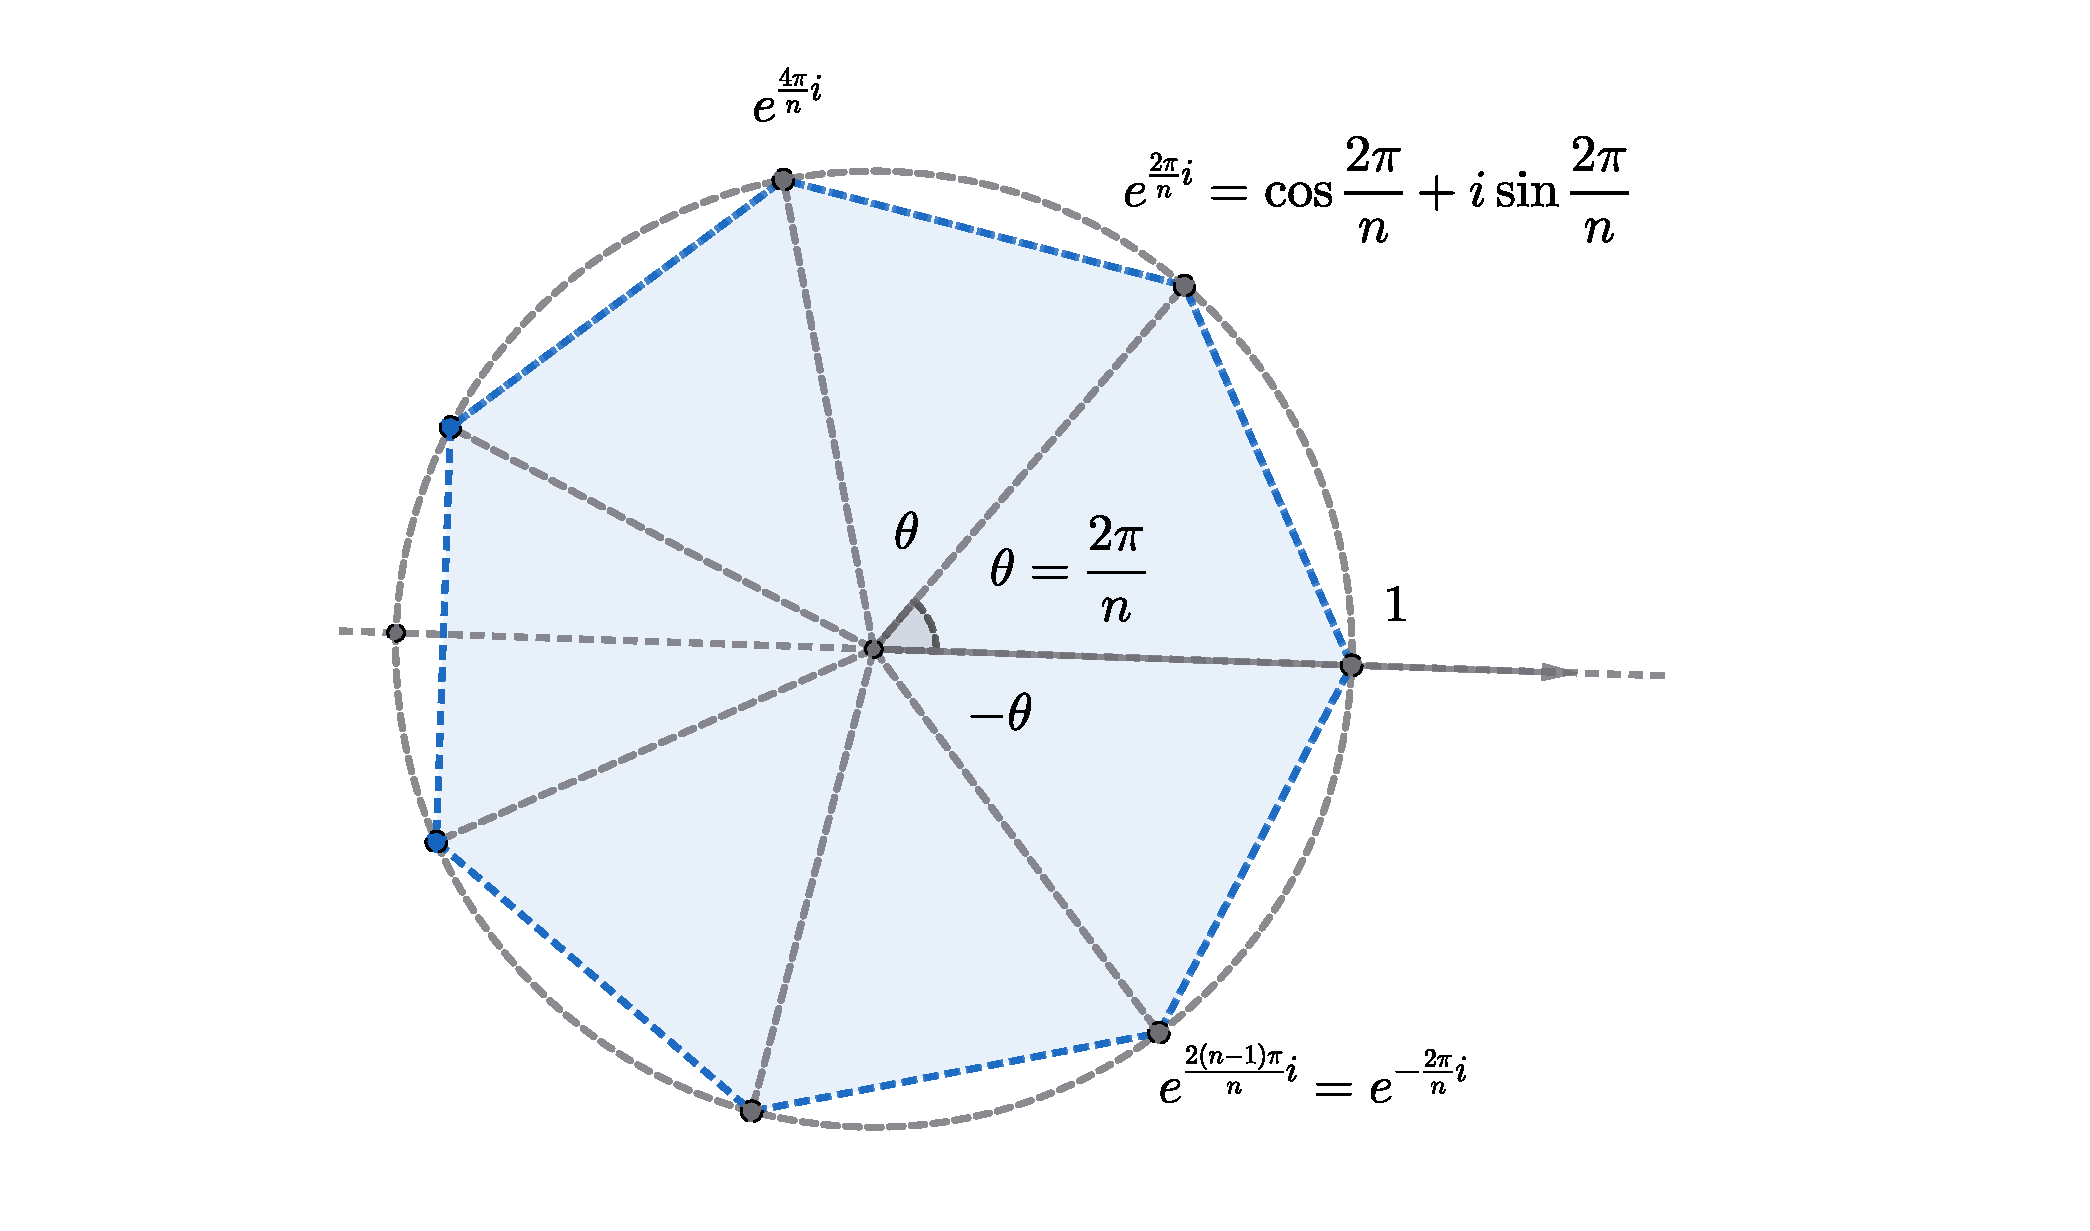
\includegraphics[scale=0.33]{img/heptagon-z}
  \caption{The roots of $x^n = 1$ are the $n$ vertices of a regular $n$-gon in the complex plane.}
 \label{fig:heptagon-z}
\end{figure}

As circle is periodic, $e^{\frac{2k\pi}{n}i}$ coincides with itself after rotating an integer number of circles. When $k = 0, 1, 2, \dotsc, n-1$, $e^{\frac{2k\pi}{n}i}$ are $n$ different roots. Their arguments are $0, \theta, 2\theta, \dotsc, (n-1)\theta$ respectively, which divides the unit circle into $n$ equal parts. Therefore, the equation $x^n = 1$ is called the "cyclotomic equation". Connecting these $n$ roots in the complex plane forms a regular $n$-gon.

The simpliest regular polygon is the equilateral triangle with $n = 3$. The equation $x^3 = 1$ has three complex roots: $1, e^{\frac{2\pi}{3}i}, e^{\frac{4\pi}{3}i} = e^{-\frac{2\pi}{3}i}$. Among them:

\[
e^{\pm \frac{2\pi}{3}i} = \cos (\pm \frac{2\pi}{3}) + i \sin (\pm \frac{2\pi}{3}) = -\frac{1}{2} \pm \frac{\sqrt{3}}{2}i
\]

One may verify that $x^3 - 1 = (x - 1)(x^2 + x + 1)$, and the two roots of the quadratic equation $x^2 + x + 1$ are indeed $\dfrac{-1 \pm i\sqrt{3}}{2}$. We can also directly verify this using binomial expansion:

\[
\left(-\frac{1}{2} \pm \frac{\sqrt{3}}{2}i\right)^3 = -\frac{1}{8} \pm \frac{3\sqrt{3}}{8}i + \frac{9}{8} \mp \frac{3\sqrt{3}}{8}i = \frac{9-1}{8} = 1
\]

The three roots on the unit circle are evenly spaced at angles of $120^\circ$ (or $\frac{2\pi}{3}$ radians), which means they form an equilateral triangle inscribed in the unit circle, as shown in \cref{fig:3rd-root-of-1}.

\begin{figure}[htbp]
\centering
\begin{tikzpicture}[scale=2.5]
 \draw[step=.5cm, gray, very thin] (-1.2,-1.2) grid (1.2,1.2);
 \draw[->] (-1.25,0) -- (1.25,0) coordinate (x axis)
   (0,-1.25) -- (0,1.25) coordinate (y axis);
 \draw (0,0) circle (1cm);
 \draw[->, very thick] (0, 0) edge node[below=2pt] {$e^0 = 1$} (1, 0)
   (0, 0) edge node[above] {$e^{\frac{2\pi}{3}i} = \dfrac{-1 + i\sqrt{3}}{2}$} (120:1cm)
   (0, 0) edge node[below] {$e^{\frac{4\pi}{3}i} = \dfrac{-1 - i\sqrt{3}}{2}$} (-120:1cm);
\end{tikzpicture}
\caption{The three complex roots of $x^3 = 1$.}
\label{fig:3rd-root-of-1}
\end{figure}

Similarly, the five roots of the equation $x^5 = 1$ are evenly spaced at angles of $72^\circ$ (or $\frac{2\pi}{5}$ radians), which means they form a regular pentagon inscribed in the unit circle, as shown in \cref{fig:pentagon-z}. Once construct the root $x$ in above figure, the distance from $x$ to 1 in the complex plane, namely $|x - 1|$, is the length of the side of the regular pentagon. The equation $x^5 - 1 = 0$ obviously has a root at $x = 1$. By the factor theorem, $x - 1$ is a factor of the polynomial $x^5 - 1$. Using polynomial long division (or reverse engineering with geometric series), we can factor it as:

\[
x^5 - 1 = (x - 1)(x^4 + x^3 + x^2 + x + 1)
\]

Next is to solve the quartic equation $x^4 + x^3 + x^2 + x + 1 = 0$ to find the remaining four vertices in \cref{fig:pentagon-z}. This quartic equation is quite special; if we divide it by $x^2$, it becomes a symmetric form (since 0 is not a root of the equation, we have $x \ne 0$):

\begin{figure}[htbp]
  \centering
  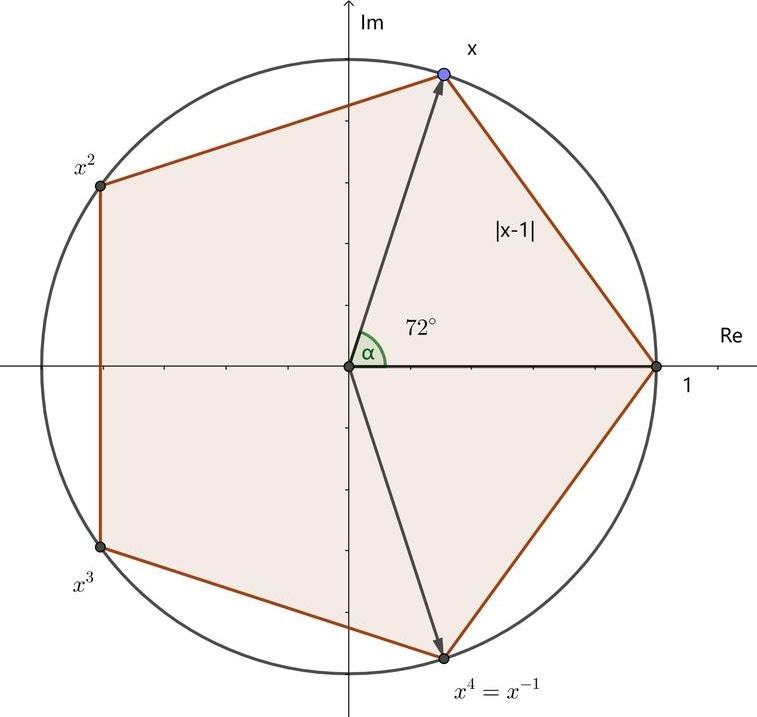
\includegraphics[scale=0.3]{img/pentagon-z}
  \caption{The roots of $x^5 = 1$ are the vertices of a regular pentagon in the complex plane.}
 \label{fig:pentagon-z}
\end{figure}

\[
x^2 + x + 1 + \frac{1}{x} + \frac{1}{x^2} = 0
\]

Treat $x + \dfrac{1}{x}$ as an unknown, and notice that: $(x + \dfrac{1}{x})^2 = x^2 + \dfrac{1}{x^2} + 2$. The above equation can be rewritten as:

\[
(x + \frac{1}{x})^2 + (x + \frac{1}{x}) - 1 = 0
\]

Let $y = x + \dfrac{1}{x}$, the above equation becomes $y^2 + y - 1 = 0$. Solving this quadratic equation gives $y_{1,2} = \dfrac{-1 \pm \sqrt{5}}{2}$. Using Euler's formula, if $x = e^{i\theta}$, then $\dfrac{1}{x} = x^{-1} = e^{-i\theta}$, so $x$ and $\dfrac{1}{x}$ are complex conjugates (see $x$ and $x^4 = x^{-1}$ in \cref{fig:pentagon-z}). If $x = a + bi$, then $\dfrac{1}{x} = a - bi$, so $x + \dfrac{1}{x} = 2a$. Similarly, $x^2$ and $x^3$ in \cref{fig:pentagon-z} are also a pair of complex conjugates, corresponding to $e^{\frac{4\pi}{5}i}, e^{\frac{6\pi}{5}i} = e^{-\frac{4\pi}{5}i}$ respectively. Thus we can determine that:

\begin{align*}
x + \dfrac{1}{x} &= \dfrac{-1 + \sqrt{5}}{2} \\
x^2 + x^3 &= \dfrac{-1 - \sqrt{5}}{2}
\end{align*}

Where the first equation is essentially a quadratic equation $x^2 - \dfrac{\sqrt{5} - 1}{2}x + 1 = 0$. Using the quadratic formula gives:

\[x_{1, 2} = \dfrac{\frac{\sqrt{5} - 1}{2} \pm i\sqrt{\frac{5 + \sqrt{5}}{2}}}{2}
\]

They are a pair of complex conjugates, corresponding to $x$ and $\dfrac{1}{x}$ in \cref{fig:pentagon-z}. We are going to figure out the modulus $|x - 1|$ in \cref{fig:pentagon-z}, which is the side length of the regular pentagon.

\[
x - 1 = \frac{\frac{\sqrt{5} - 1}{2} + i\sqrt{\frac{5 + \sqrt{5}}{2}}}{2} - 1 = \frac{\sqrt{5} - 5}{4} + i\frac{\sqrt{\frac{5 + \sqrt{5}}{2}}}{2}
\]

Therefore,

\[
|x - 1| = \sqrt{\left(\frac{\sqrt{5} - 5}{4}\right)^2 + \left(\frac{\sqrt{\frac{5 + \sqrt{5}}{2}}}{2}\right)^2} = \frac{\sqrt{10 - 2\sqrt{5}}}{2}
\]

The problem of construction of a regular pentagon is turned into: given a line segment of length 1, how to construct a line segment of length $s = \dfrac{\sqrt{10 - 2\sqrt{5}}}{2}$. To simplify the problem, we first find the line segment of length $2s$. Our idea is to construct a right triangle with its hypotenuse being $2s$. The two legs of this triangle cannot both be rational numbers, otherwise according to the Pythagorean theorem, the hypotenuse cannot be in the form of $\sqrt{10 - 2\sqrt{5}}$ which has a square root under another square root. Let the two legs be $\sqrt{5} - a$ and $b$, then using the Pythagorean theorem:

\[
(\sqrt{5} - a)^2 + b^2 = 5 + a^2 + b^2 - 2a\sqrt{5} = 10 - 2\sqrt{5}
\]

Equating the irrational part on both sides, $2a = 2$, so $a = 1$. Substituting back into the equation gives $5 + a^2 + b^2 = 6 + b^2 = 10$, so $b = 2$. Thus, the right triangle with legs $\sqrt{5} - 1$ and $2$ has a hypotenuse of $2s$. Scaling down this triangle by half gives a right triangle with legs $\dfrac{\sqrt{5} - 1}{2}$ and $1$, whose hypotenuse is $s$. On the other hand, since $5 = 4 + 1 = 2^2 + 1^2$, we can construct a right triangle with legs of length 1 and 2, and its hypotenuse is $\sqrt{5}$. Scaling down this triangle by half gives a right triangle with hypotenuse $\dfrac{\sqrt{5}}{2}$, and then cutting off $\dfrac{1}{2}$ gives us $\dfrac{\sqrt{5} - 1}{2}$. \cref{fig:pentagon-cons} shows the steps for constructing a regular pentagon. Finally, using the obtained side length to cut the unit circle five times gives us the regular pentagon.

\begin{figure}[htbp]
 \centering
 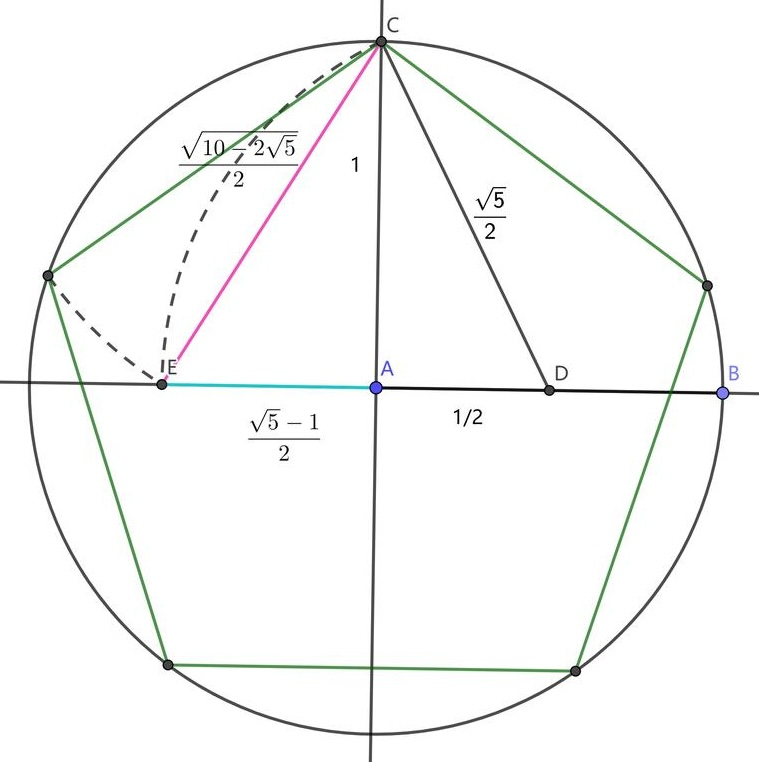
\includegraphics[scale=0.3]{img/pentagon-cons}
 \caption{Construction of a regular pentagon}
 \label{fig:pentagon-cons}
\end{figure}

\begin{Exercise}[label={ex:complex}]
\Question{Give the geometric interpretation to the quadratic equation $x^2 - px = q$. \label{qn:geometric-quadratic}}

\Question{By the foundamental theorem of algebra, a cubic equation has three complex roots. Cardano's formula gives one root of the equation $x^3 = 6x + 9$ as $x_1 = 3$. Find the other two roots of the equation.}

\Question{Using Bombelli's method and Cardano's formula, one root of the equation $x^3 = 15x + 4$ is $x_1 = 4$. Find the other two roots of the equation.}

\Question{Is the rule $\sqrt{ab} = \sqrt{a}\sqrt{b}$ valid in complex numbers? If so, prove it; if not, how can it be salvaged? \label{qn:sqrt-of-product}}

\Question{Show that multiplying any complex number represented as a vector by $i$ is equivalent to rotating the vector by $90\degree$ counterclockwise. \label{qn:mul-i}}

\Question{Verify that the conjugate of a complex number satisfies the following rules: $\overline{a + b} = \overline{a} + \overline{b}$, $\overline{ab} = \overline{a} \cdot \overline{b}$, $\overline{z^n} = (\overline{z})^n$, and use these rules to prove d'Alembert's discovery: if $z$ is a root of the equation $p(z) = 0$, then its conjugate $\overline{z}$ is also a root of the equation. \label{qn:conjugated-root}}

\Question{Verify that Hamilton's representation of complex numbers as ordered pairs satisfies the five fundamental arithmetic rules. \label{qn:pair-arithmetic-rules}}

\Question{Use the fact that logarithmic function and exponential function are inverse functions to prove the change of base formula $\log_a x = \dfrac{\log_b x}{\log_b a}$. \label{qn:change-base}}

\Question{*Use the polar equation of equiangular spiral $r = ke^{b\theta}$ to prove the equiangular property pointed out by Descartes: the angle $\Psi$ between the tangent and the radial line is constant (see \cref{fig:equiangular}). Hint: as shown in \cref{fig:tagent-to-r}, when the radial line $r$ rotates through a small angle $\Delta \theta$, it increases by $\Delta r$. The small arc $AC$ has length $r\Delta \theta$, and it, together with the secant $AB$ and the increment of radial line, approximately forms a right triangle $ACB$. When $\Delta \theta \to 0$, points $A, B$ approach each other, and the secant $AB$ approaches the tangent.

  \begin{center}
    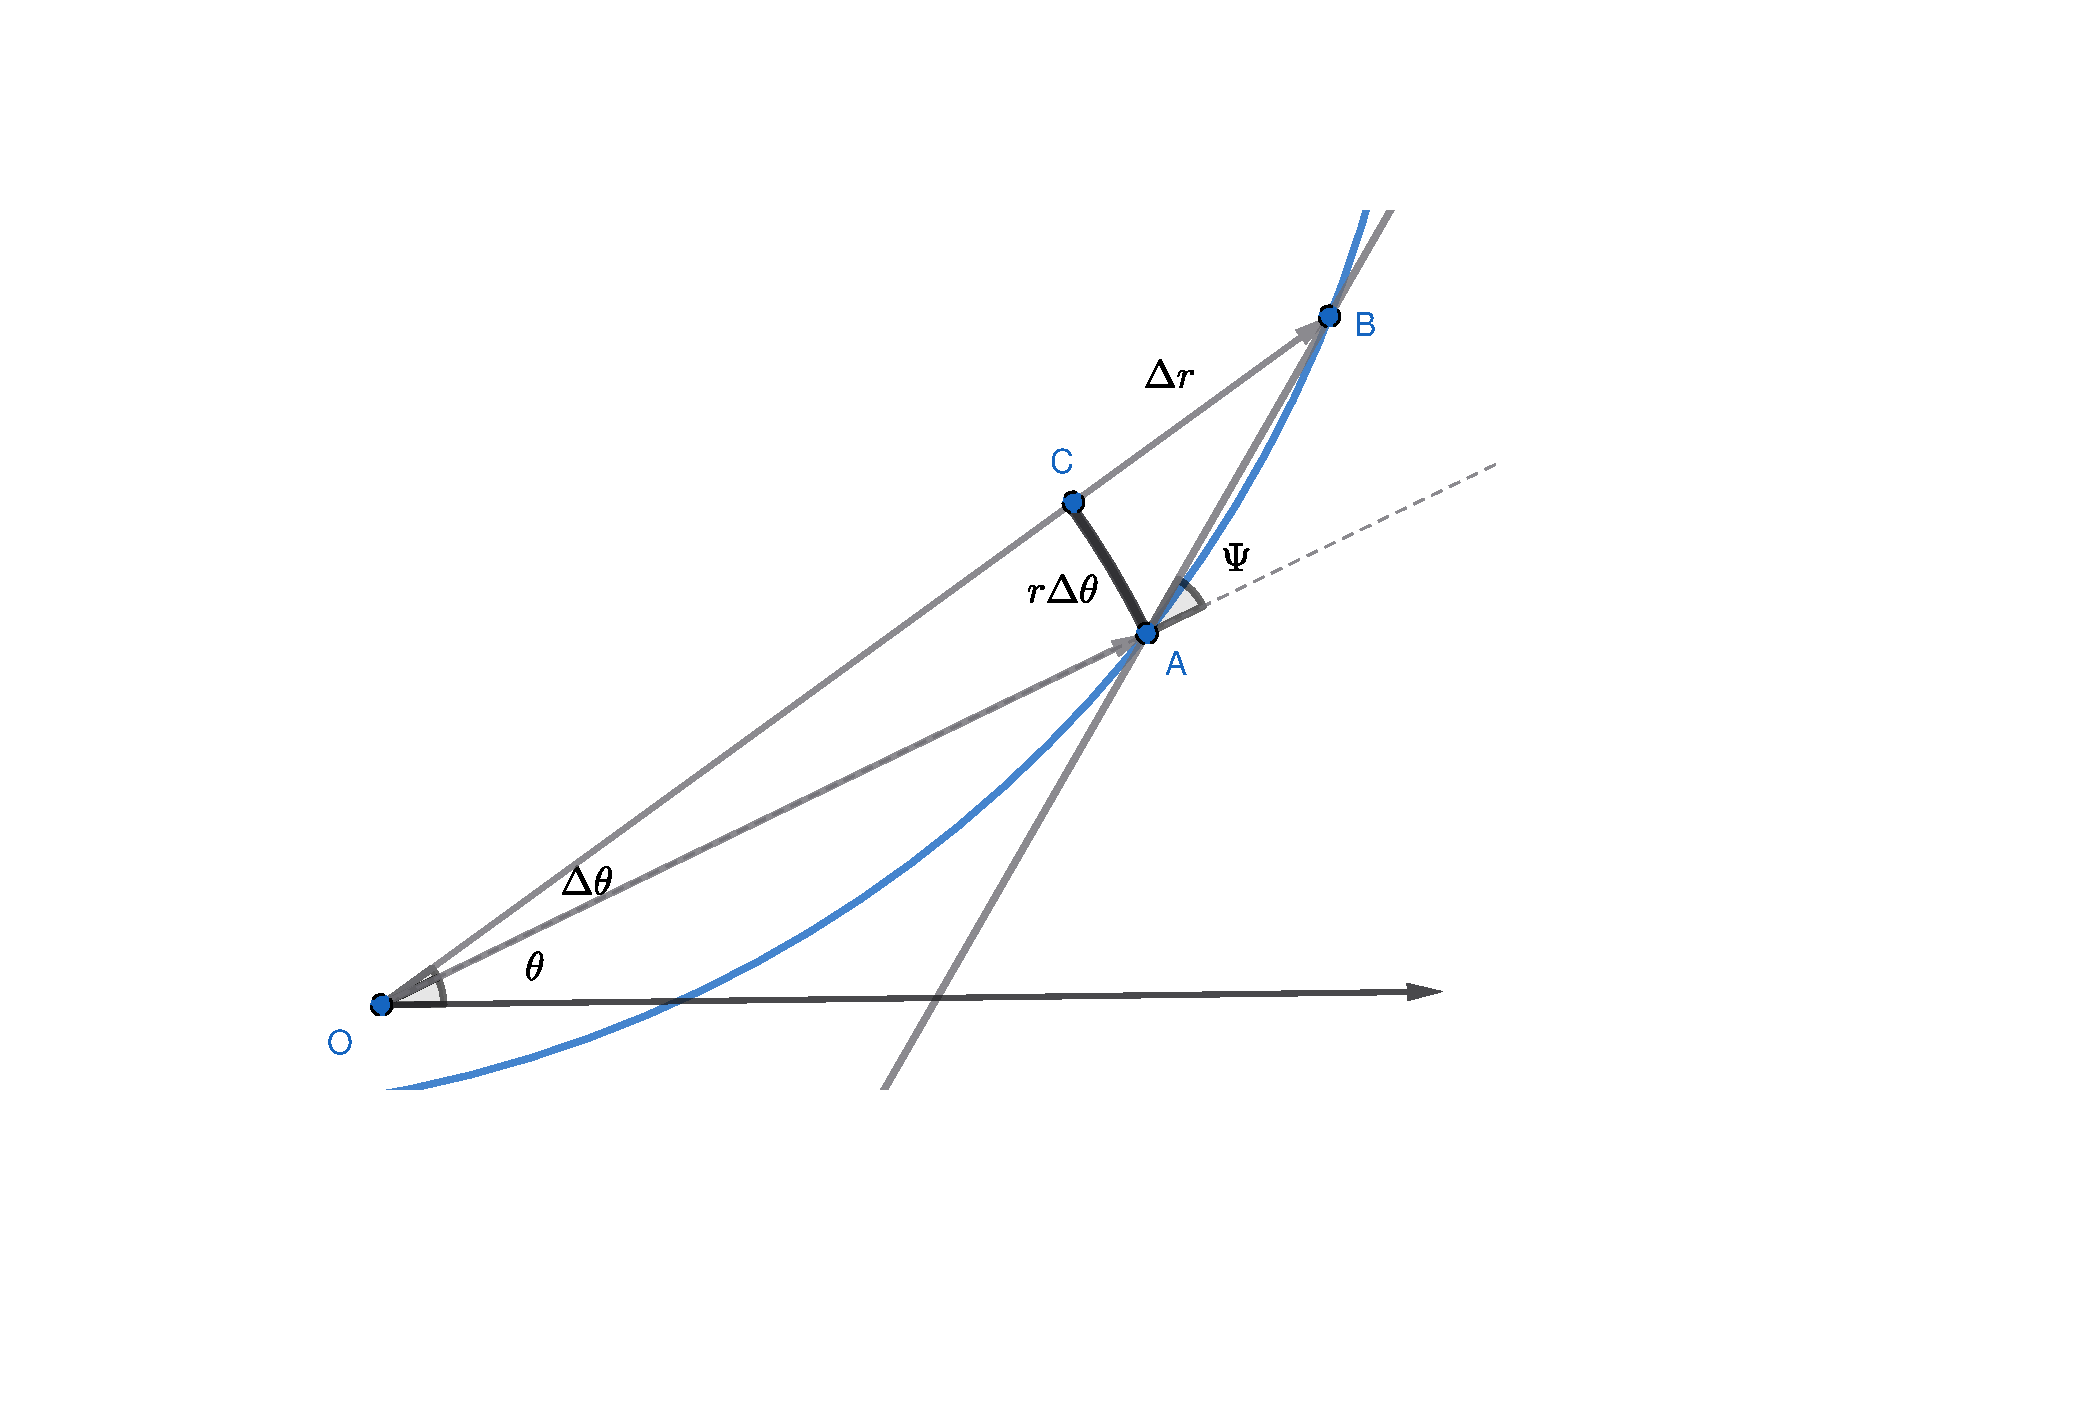
\includegraphics[scale=0.33]{img/tagent-to-r}
    \captionof{figure}{Radial line rotates through a small angle $\Delta \theta$}
    \label{fig:tagent-to-r}
  \end{center}
}

\Question{*Jacob Bernoulli's epitaph, \enquote{Eadem mutata resurgo}, describes the property of the derivative of $e^x$ being unchanged, $(e^x)' = e^x$. Modern mathematicians define the function $f(x) = e^x$ as follows: (1) the derivative is unchanged, $f'(x) = f(x)$, (2) the function value at 0 is 1, $f(0) = 1$. Use this definition to derive the expansion of $e^x$. Hint: method of undetermined coefficients and $(x^n)' = nx^{n-1}$ (see Proposition \ref{thm:derivation-of-power-of-x}). \label{qn:exp-from-fixed-point}}

\Question{*Jacob Bernoulli's discovery of the distance to $e^x$ is almost one step away. When calculating compound interest, if the annual interest rate is not 100\% but $x$, what is the actual annualized return when $n \to \infty$? What is its series expansion? \label{qn:compound-interest}}

\Question{Show the trigonometric addition formulas $\tan(\theta_1 + \theta_2), \sin(\theta_1 + \theta_2), \cos(\theta_1 + \theta_2)$ using complex numbers. Hint: complex multiplication. \label{qn:trigonometry-of-add}}

\end{Exercise}

\begin{Answer}[ref={ex:complex}]
\Question{Give the geometric interpretation to the quadratic equation $x^2 - px = q$.

\vspace{2mm}
\begin{center}
 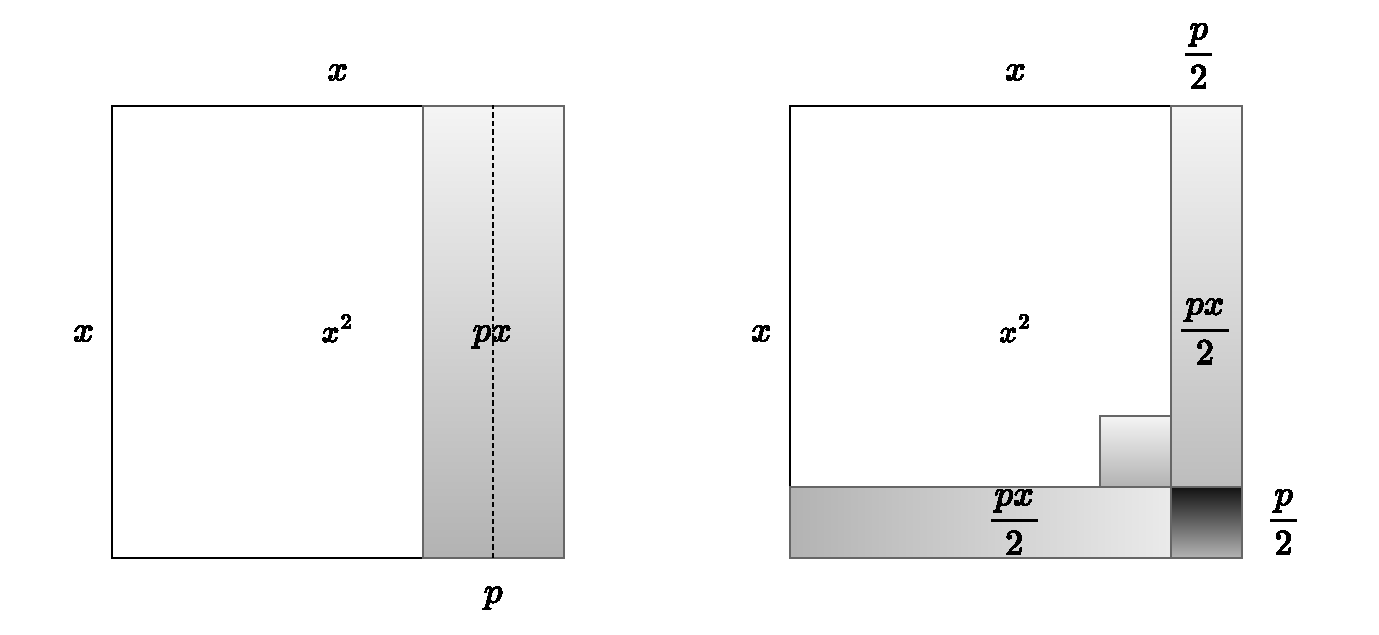
\includegraphics[scale=0.5]{img/quadratic3}
 \captionof{figure}{Left: cut a rectangle of area $px$ from a square of area $x^2$; Right: the white area is equal, $q = (x - \dfrac{p}{2})^2 - (\dfrac{p}{2})^2$.}
\end{center}
}

\Question{By the foundamental theorem of algebra, a cubic equation has three complex roots. Cardano's formula gives one root of the equation $x^3 = 6x + 9$ as $x_1 = 3$. Find the other two roots of the equation.

\vspace{2mm}
Factor the equation as $x^3 - 6x - 9 = 0$. By Descartes' theorem, $x - 3$ is a factor of the polynomial $x^3 - 6x - 9$. Using polynomial long division or the method of undetermined coefficients, we can factor it as:

\[
\polylongdiv{x^3-6x-9}{x-3}
\]

Which gives $x^2 + 3x + 3$.

Alternatively, equating the coefficients:

\begin{align*}
x^3 - 6x - 9 &= (x - 3)(x^2 + ax + b) \\
  &= x^3 + ax^2 + bx - 3x^2 - 3ax - 3b \\
  &= x^3 + (a - 3)x^2 + (b - 3a)x - 3b
\end{align*}

Hence, $a = 3, b = 3$. Solving the quadratic equation $x^2 + 3x + 3 = 0$ gives the other two roots $x_{2, 3} = \dfrac{-3 \pm i\sqrt{3}}{2}$.
}

\Question{Using Bombelli's method and Cardano's formula, one root of the equation $x^3 = 15x + 4$ is $x_1 = 4$. Find the other two roots of the equation.

\vspace{2mm}
As in the previous exercise, factor the polynomial as $x^3 - 15x - 4 = 0$. By Descartes's theorem, $x - 4$ is a factor. Using polynomial long division,

\[
\polylongdiv{x^3-15x-4}{x-4}
\]

Or equating the coefficients:

\begin{align*}
x^3 - 15x - 4 &= (x - 4)(x^2 + ax + b) \\
  &= x^3 + ax^2 + bx - 4x^2 - 4ax - 4b \\
  &= x^3 + (a - 4)x^2 + (b - 4a)x - 4b
\end{align*}

Hence $a = 4, b = 1$. Solving the quadratic equation $x^2 + 4x + 1 = 0$ gives the other two roots $x_{2, 3} = -2 \pm \sqrt{3}$
}

\Question{Is the rule $\sqrt{ab} = \sqrt{a}\sqrt{b}$ valid in complex numbers? If so, prove it; if not, how can it be salvaged?

\vspace{2mm}
No, it's invalid, otherwise,
\[
ab = \sqrt{a^2b^2} = \sqrt{(-a^2)(-b^2)} = \sqrt{-a^2}\sqrt{-b^2} = (ai)(bi)=-ab
\]

A contradiction arises when $ab \ne 0$. In complex numbers, we can either follow Euler's approach and define $\sqrt{a}$ as $b$ such that $b^2 = a$, which means $\pm\sqrt{a}$; or we can let $z^2 = ab, x^2 = a, y^2 = b$, so that $z^2 = x^2y^2 = (xy)^2$. For example:

\[
36 = 4 \times 9 = (-4)\times(-9) = (2i)^2(3i)^2 = (2i \times 3i)^2 = (-6)^2 = 36
\]
}

\Question{Show that multiplying any complex number represented as a vector by $i$ is equivalent to rotating the vector by $90\degree$ counterclockwise.

\begin{proof}
For any complex number $z = a + bi$, if $a = 0$ and $b \ne 0$, then $z = bi$, and $zi = -b$. If $b > 0$, the vector rotates from the positive direction of the imaginary axis to the negative direction of the real axis, which is a left turn of 90 degrees; if $b < 0$, the vector rotates from the negative direction of the imaginary axis to the positive direction of the real axis, which is also a left turn of 90 degrees.

If $a \ne 0, b = 0$, then $z = a, zi = ai$. If $a > 0$, the vector rotates from the positive direction of the real axis to the positive direction of the imaginary axis, which is a left turn of 90 degrees; if $a < 0$, the vector rotates from the negative direction of the real axis to the negative direction of the imaginary axis, which is also a left turn of 90 degrees.

If $ab \ne 0$, then $zi = (a + bi)i = ai - b$. Let $\theta = arg(z), \psi = arg(zi)$, we have:

\[
\tan \theta \tan \psi = (b/a)(-a/b) = -1
\]

Hence $\psi = \theta + \dfrac{\pi}{2}$, a left turn of 90 degrees.
\end{proof}
}

\Question{Verify that the conjugate of a complex number satisfies the following rules: $\overline{a + b} = \overline{a} + \overline{b}$, $\overline{ab} = \overline{a} \cdot \overline{b}$, $\overline{z^n} = (\overline{z})^n$, and use these rules to prove d'Alembert's discovery: if $z$ is a root of the equation $p(z) = 0$, then its conjugate $\overline{z}$ is also a root of the equation.

\begin{proof}
Conjugate of sum:
    \begin{align*}
    \overline{a + b} &= \overline{p + qi + r + si} && \text{令}a = p + qi, b = r + si \\
      &= \overline{p + r + (q + s)i} = p + r - (q + s)i &&\text{共轭的定义} \\
      &= p - qi + r - si = \overline{a} + \overline{b}
    \end{align*}
Conjugate of product:
    \begin{align*}
    \overline{ab} &= \overline{(p + qi)(r + si)} \\
      &= \overline{pr - qs + (ps + qr)i} = pr - qs - (ps + qr)i
    \end{align*}
Product of conjugation:
    \begin{align*}
    \overline{a} \cdot \overline{b} &= (p - qi)(r - si) = pr - qs - (ps + qr)i \\
      &= \overline{ab}
    \end{align*}
Let $b = a$ and substitute into the product of conjugation, repeat $n$ times to get $\overline{a^n} = (\overline{a})^n$.

If $z$ is a root of the equation $p(x) = a_nx^n + \dotsb + a_1 x + a_0 = 0$, then substitute $z$ into,

\begin{align*}
0 &= a_nz^n + \dotsb + a_1 z + a_0 \\
\overline{0}  &= \overline{a_nz^n + \dotsb + a_1 z + a_0} && \text{conjugate}\\
0 &= \overline{a_nz^n} + \dotsb + \overline{a_1 z} + \overline{a_0} && \text{conjugate of sum}\\
  &= \overline{a_n}\overline{z^n} + \dotsb + \overline{a_1}\overline{z} + \overline{a_0} && \text{conjugate of product}\\
  &= \overline{a_n}(\overline{z})^n + \dotsb + \overline{a_1}\overline{z} + \overline{a_0} && \text{conjugate of power}\\
  &= a_n(\overline{z})^n + \dotsb + a_1\overline{z} + a_0 && \text{conjugate of real numbers} \\
  &= p(\overline{z}) && \qedhere
\end{align*}
\end{proof}
}

\Question{Verify that Hamilton's representation of complex numbers as ordered pairs satisfies the five fundamental arithmetic rules.

\begin{proof}
Commutativity of addition:
\begin{align*}
(a, b) + (c, d) &= (a + c, b + d) && \text{sum of pair} \\
  &= (c + a, d + b) && \text{addition is commutative for normal numbers} \\
  &= (c, d) + (a, b) && \text{sum of pair, reverse}
\end{align*}

Commutativity of multiplication:
\begin{align*}
(a, b)(c, d) &= (ac - bd, bc + ad) && \text{product of pair} \\
  &= (ca - db, cb + da) && \text{multiplication is commutative for normal numbers} \\
  &= (c, d)(a, b) && \text{product of pair, reverse}
\end{align*}

Associativity of addition:
\begin{align*}
(a, b) + (c, d) + (e, f) &= (a + c, b + d) + (e, f) \\
  &= (a + c + e, b + d + f) \\
  &= (a + (c + e), b + (d + f)) && \text{associativity for normal numbers} \\
  &= (a, b), (c + e, d + f) \\
  &= (a, b) + [(c, d) + (e, f)] && \text{sum of pair, reverse}
\end{align*}

Associativity of multiplication:
\begin{align*}
(a, b)(c, d)(e, f) &= (ac - bd, ad + bc)(e, f) \\
  &= ((ac - bd)e - (ad + bc)f, (ac - bd)f + (ad + bc)e) \\
  &= (ace - bde - adf - bcf, acf - bdf + ade + bce) \\
\text{on the other hand} \\
(a, b)[(c, d)(e, f)] &= (a, b)(ce - df, cf + de)) \\
  &= (a(ce - df) - b(cf + de), a(cf + de) + b(ce - df)) \\
  &= (ace - adf - bcf - bde, acf + ade + bce - bdf) \\
  &= (ace - bde - adf - bcf, acf - bdf + ade + bce) \\
  &= (a, b)(c, d)(e, f)
\end{align*}

Left distribution:
\begin{align*}
(a, b)[(c, d) + (e, f)] &= (a, b)(c + e, d + f) \\
  &= (a(c + e) - b(d + f), a(d + f) + b(c + e)) \\
  &= (ac + ae - bd - bf, ad + af + bc + be) \\
  &= (ac - bd + (ae - bf), ad + bc + (af + be)) \\
  &= (ac - bd, ad + bc) + (ae - bf, af + be) \\
  &= (a, b)(c, d) + (a, b)(e, f)
\end{align*}
Right distribution holds by the commutativity of multiplication.
\end{proof}
}

\Question{Use the fact that logarithmic function and exponential function are inverse functions to prove the change of base formula.

  \begin{proof}
    \begin{align*}
      y &= \log_a x && a \ne 1 \\
      a^y &= x && \text{inverse function} \\
      log_b (a^y) &= log_b x && \text{take logarithm of base }b\text{ for both sides} \\
      y log_b a &= log_b x && \text{rule of logarithm} \\
      y &= \frac{log_b x}{log_b a} && a \ne 1\text{, the denominator is not zero} \qedhere
    \end{align*}
  \end{proof}
}

\Question{*Use the polar equation of equiangular spiral $r = ke^{b\theta}$ to prove the equiangular property pointed out by Descartes: the angle $\Psi$ between the tangent and the radial line is constant (see \cref{fig:equiangular}).

  \begin{center}
    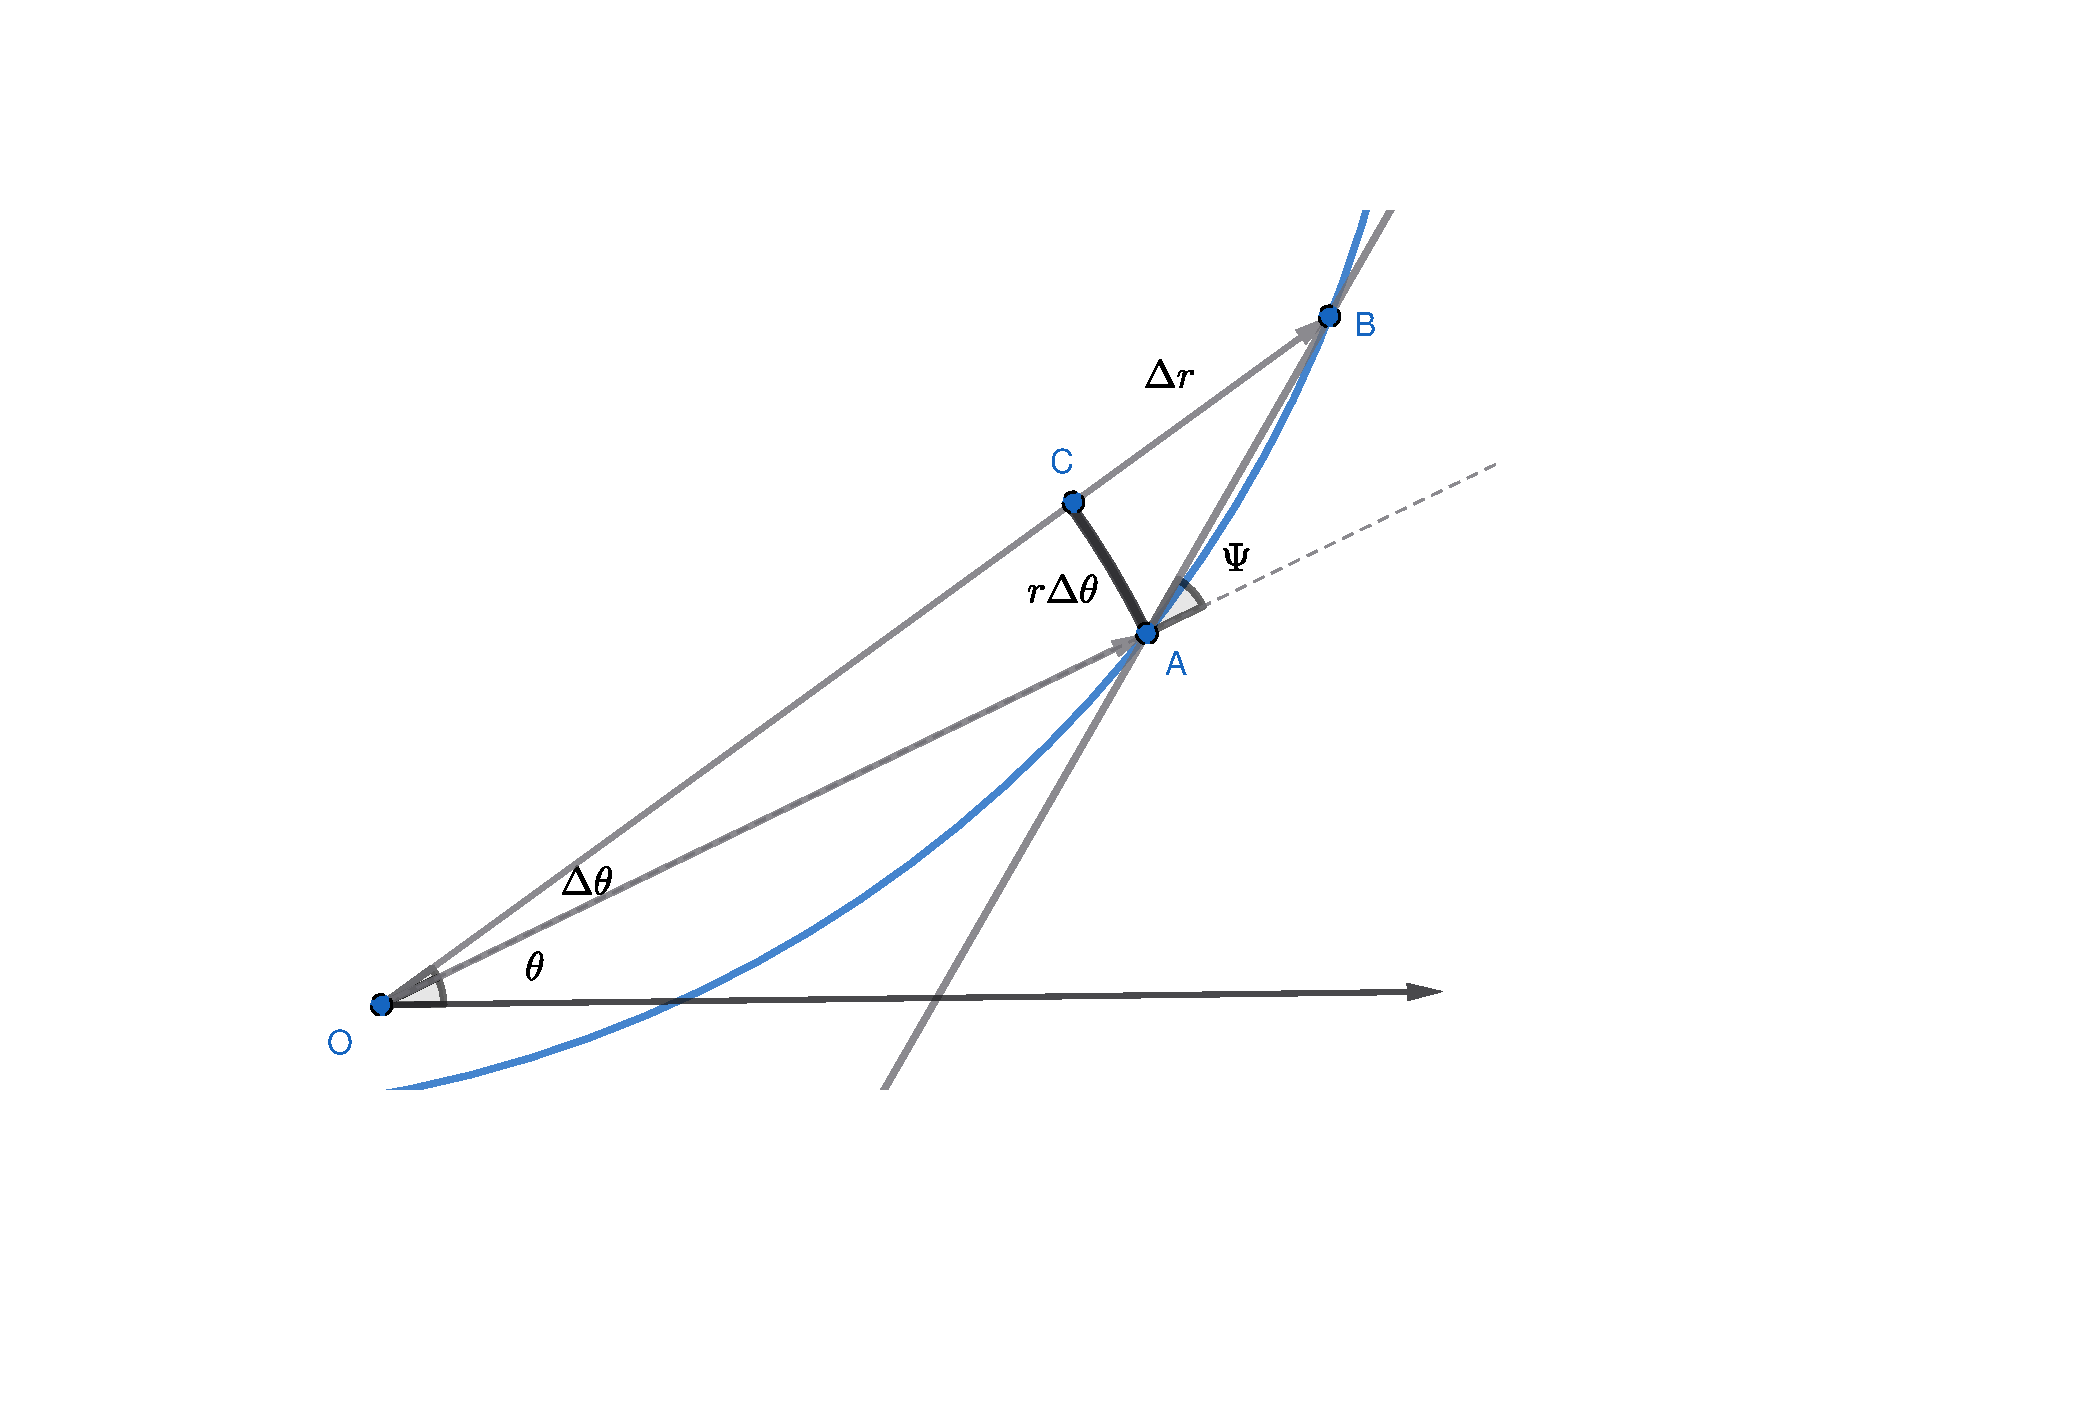
\includegraphics[scale=0.33]{img/tagent-to-r}
    \captionof{figure}{Radial line rotates through a small angle $\Delta \theta$.}
    \label{fig:tagent-to-ra}
  \end{center}

  \begin{proof}
As shown in \cref{fig:tagent-to-ra}, when the radial line $r$ rotates through a small angle $\Delta \theta$, its length increases by $\Delta r$. The length of the small arc $AC$ is $r\Delta \theta$; this arc together with the secant $AB$, the increment of the radial line form a roughly right triangle $ACB$. When $\Delta \theta \to 0$, the two points $A, B$ close to each other, and the secant $AB$ approximates the tagent. The angle $ABC = \Psi - \Delta \theta$.

\begin{align*}
  \tan \Psi &= \lim_{\Delta \theta \to 0} \tan (\Psi - \Delta \theta) = \lim_{\Delta \theta \to 0} \tan \angle ABC \\
  &= \lim_{\Delta \theta \to 0} \frac{r\Delta \theta}{\Delta r} = \lim_{\Delta \theta \to 0} \frac{r}{\frac{\Delta r}{\Delta \theta}} \\
  &= \frac{r}{\lim_{\Delta \theta \to 0} \dfrac{\Delta r}{\Delta \theta}} = \frac{r}{r'} = \frac{ke^{b\theta}}{(ke^{b\theta})'} && \text{代入}r = ke^{b\theta} \\
  &= \frac{ke^{b\theta}}{kbe^{b\theta}} = \frac{1}{b} && (e^{bx})' = be^{bx}
\end{align*}
This is a constant independant of $\theta$, which proves the equiangular property of the spiral.
  \end{proof}
}

\Question{*Jacob Bernoulli's epitaph, \enquote{Eadem mutata resurgo}, describes the property of the derivative of $e^x$ being unchanged, $(e^x)' = e^x$. Modern mathematicians define the function $f(x) = e^x$ as follows: (1) the derivative is unchanged, $f'(x) = f(x)$, (2) the function value at 0 is 1, $f(0) = 1$. Use this definition to derive the expansion of $e^x$.

\vspace{2mm}
Let the expansion of of $e^x$ be $f(x) = a_0 + a_1 x + a_2 x^2 + \dotsb$. By $f(0) = 1$, hence $f(0) = a_0 = 1$. Taking the derivative and by $f'(x) = f(x)$,
\begin{align*}
f'(x) &= a_1 + 2a_2x + 3a_3x^2 + \dotsb + na_nx^{n-1} + \dotsb = f(x) \\
      &= 1 + a_1x + a_2x^2 + \dotsb + a_{n-1}x^{n-1} + \dotsb
\end{align*}
Equating the coefficients:
\begin{align*}
a_1 &= 1\\
a_2 &= \frac{a_1}{2} = \frac{1}{2}\\
a_3 &= \frac{a_2}{3} = \frac{a_1}{3 \cdot 2} = \frac{1}{3!}\\
\dotso\\
a_n &= \frac{a_{n-1}}{n} = \frac{a_{n-2}}{n(n-1)} = \dotsb = \frac{1}{n!} \\
\dotso
\end{align*}

Therefore, the expansion of $e^x$ is,
\begin{align*}
e^x &= f(x) = 1 + x + \frac{x^2}{2!} + \frac{x^3}{3!} + \dotsb + \frac{x^n}{n!} + \dotsb
\end{align*}
}

\Question{*Jacob Bernoulli's discovery of the distance to $e^x$ is almost one step away. When calculating compound interest, if the annual interest rate is not 100\% but $x$, what is the actual annualized return when $n \to \infty$? What is its series expansion?

\vspace{2mm}
\begin{align*}
\lim_{n \to \infty} (1 + \frac{x}{n})^n &= \lim_{n \to \infty} (1 + \frac{x}{n})^{\frac{n}{x}x} && \text{其中} x \ne 0 \\
  &= [\lim_{n' \to \infty} (1 + \frac{1}{n'})^{n'}]^x && \text{令} n' = \frac{n}{x} \\
  &= e^x
\end{align*}

By the general binomial theorem,
\begin{align*}
e^x &= \lim_{n \to \infty} (1 + \frac{x}{n})^n \\
  &= \lim_{n \to \infty} (1 + \binom{n}{1}\frac{x}{n} + \binom{n}{2}\frac{x^2}{n^2} + \dotsb \\
  &= \lim_{n \to \infty} (1 + x + \frac{n(n-1)}{2!}\frac{x^2}{n^2} + \dotsb \\
  &= \lim_{n \to \infty} (1 + x + \frac{x^2}{2!}(1-\frac{1}{n}) + \frac{x^3}{3!}(1 - \frac{1}{n})(1 - \frac{2}{n}) + \dotsb \\
  &= 1 + x + \frac{x^2}{2!} + \frac{x^3}{3!} + \dotsb
\end{align*}
}

\Question{Show the trigonometric addition formulas $\tan(\theta_1 + \theta_2), \sin(\theta_1 + \theta_2), \cos(\theta_1 + \theta_2)$ using complex numbers.

\vspace{2mm}

For two complex numbers $z_1 = a_1 + b_1i, z_2 = a_2 + b_2i$, their arguments are $\theta_1 = \tan^{-1} \dfrac{b_1}{a_1}, \theta_2 = \tan^{-1} \dfrac{b_2}{a_2}$ respectively (suppose the real part isn't 0), and their moduli are $r_1 = \sqrt{a_1^2 + b_1^2}, r_2 = \sqrt{a_2^2 + b_2^2}$ respectively. Their product is,

\[
z_1z_2 = (a_1 + b_1i)(a_2 + b_2i) = a_1a_2 - b_1b_2 + (a_1b_2 + b_1a_2)i
\]

By the geometric interpretation of complex numbers, the argument of the product is $arg(z_1z_2) = \theta_1 + \theta_2$, and the modulus is $|z_1z_2|= r_1r_2$.

\begin{align*}
\tan(\theta_1 + \theta_2) &= \tan(arg(z_1z_2)) = \frac{a_1b_2 + b_1a_2}{a_1a_2 - b_1b_2} && \text{suppose the denominator isn't 0} \\
  &= \dfrac{\dfrac{b_2}{a_2} + \dfrac{b_1}{a_1}}{1 - \dfrac{b_1}{a_1}\dfrac{b_2}{a_2}} && \text{both divided by }a_1a_2 \\
  &= \frac{\tan\theta_2 + \tan\theta_1}{1 - \tan\theta_1 \tan\theta_2}
\end{align*}

Similarly, by $\sin(\theta_1 + \theta_2) = \dfrac{a_1b_2 + b_1a_2}{r_1r_2}$, one can derive the analogous formulas for sine and cosine.

\begin{align*}
\sin(\theta_1 + \theta_2) &= \sin(arg(z_1z_2)) = \frac{a_1b_2 + b_1a_2}{r_1r_2} && \text{suppose the denominator isn't 0} \\
  &= \frac{a_1}{r_1}\frac{b_2}{r_2} + \frac{b_1}{r_1}\frac{a_2}{r_2} \\
  &= \cos\theta_1 \sin\theta_2 + \sin\theta_1 \cos\theta_2
\end{align*}

\begin{align*}
\cos(\theta_1 + \theta_2) &= \cos(arg(z_1z_2)) = \frac{a_1a_2 - b_1b_2}{r_1r_2} && \text{suppose the denominator isn't 0} \\
  &= \frac{a_1}{r_1}\frac{a_2}{r_2} - \frac{b_1}{r_1}\frac{b_2}{r_2} \\
  &= \cos\theta_1 \cos\theta_2 - \sin\theta_1 \sin\theta_2
\end{align*}
}

\end{Answer}

\ifx\wholebook\relax
\chapter{Algebraic numbers}
\else
\section{Algebraic numbers}
\fi

%% For English version, use Kronecker's saying ``God made the natural numbers, the rest is the work of man.''
\epigraph{Mathematics constructs an ideal world where everything is perfect and yet true.}{Bertrand Russell}
%% "The meaning of the world is the separation of wish and fact. Wish is a force as applied to thinking beings, to realize something. A fulfilled wish is a union of wish and fact. The meaning of the whole world is the separation and the union of fact and wish". [9.4.3]
%%  Hao Wang’s supplemental biography of Gödel, A Logical Journey, MIT Press, 1996.

\label{sec:FLT-4} \index{Fermat's Last Theorem!n=4}
The renowned Fermat's Last Theorem, abbreviated as FLT, states there is no solution in nonzero integers to the equation $x^n + y^n = z^n$ for integer $n \geq 3$. Although Fermat complained that the margin was too small to contain his proof, he later did proved the case of $n = 4$, that $x^4 + y^4 = z^4$ has no solution in positive integers. Fermat developed a technique called \emph{infinite descent} in this proof, and he was very proud of it. Indeed, mathematicians in the later 200 years almost all followed Fermat's method for other cases\citepage[p40-42]{Edward-1977}. Fermat found it's sufficient to prove below lemma for the case of $n = 4$\citepage[p247]{Hardy2009}.

\begin{lemma}
The equation $x^4 + y^4 = z^2$ has no solution in positive integers.
\end{lemma}

Indeed, if equation $x^4 + y^4 = u^4$ has a solution, let $z = u^2$, then it is also the solution to $x^4 + y^4 = z^2$.

\begin{proof}
Assume for contradiction, that $x^4 + y^4 = z^2$ has some solution in positive integers. Fermat further assumed $x, y, z$ were coprime of each other. Otherwise if any two have some common divisor $d \ne 1$, then it is also a divisor of the other (see \cref{qn:xyz-coprime}), which can be canceled from the both sides of the equation. Since $x^2, y^2, z$ form a Pythagorean triple, by Euclid's lemma \ref{thm:pythagoras-triples},

\begin{align*}
x^2 &= 2mn \\
y^2 &= m^2 - n^2 \\
z &= m^2 + n^2
\end{align*}

where $m > n$, they are coprime and in different parity. Convert the second equation to $y^2 + n^2 = m^2$; since $m, n$ are coprime, $y, n, m$ turn out to be a Pythagorean triple, where $m$ is odd, $y$ is odd, $n$ is even. Apply Euclid's lemma again:

\begin{align*}
n &= 2ab \\
y &= a^2 - b^2 \\
m &= a^2 + b^2
\end{align*}

where $a > b$, the are coprime and in different parity. Substitute into $x^2 = 2mn = 4ab(a^2 + b^2)$, which implies $ab(a^2 + b^2)$ is a square. But $ab$ and $a^2 + b^2$ are coprime (if any prime number $p$ divides $ab$, then $p$ divides $a$ or $b$; but since $a, b$ are coprime, $p$ can't divides both $a$ and $b$, hence $p$ does not divide $a^2 + b^2$), it follows that both are squares (see \cref{qn:coprime-product-as-square}). Let $a^2 + b^2 = Z^2$. Since $a, b$ are coprime, if $ab$ is a square, then both $a$ and $b$ are squares. Let $a = X^2, b= Y^2$, it follows that $X^4 + Y^4 = a^2 + b^2 = Z^2$.

Compare $X^4 + Y^4 = Z^2$ with the original equation $x^4 + y^4 = z^2$. They are in the same form, and,
\[
Z < Z^2 = a^2 + b^2 = m < m^2 + n^2 = z
\]

It generates smaller and smaller positive integers of $z$ infinitely (infinite descent), which is impossible.
\end{proof}

\index{infinite descent}
Fermat's method of infinite descent is essentially a proof by contradiction. One deduces from the original form of $f(x)$, by assumption, to the same form of $f(X)$ for positive integers $x > X > 0$. However, from any finite positive number, it impossible to produce infinite descent of positive numbers, which contradict with the assumption. \Cref{fig:infinite-descent} illustrates the method of descent. A bolt remains $x$ rotations of screw to the ground, after twisting for a while, there remains $X$ rotations left, where $x > X > 0$ are positive integers. However, the number of rotations of a bolt is finite, it is impossible to twisting infinitely.

\begin{figure}[htbp]
 \centering
 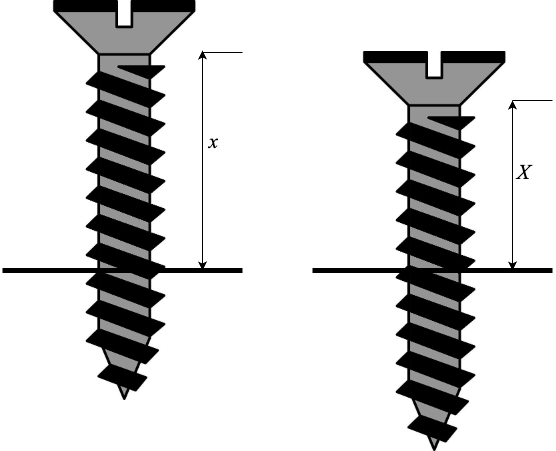
\includegraphics[scale=0.3]{img/infinite-descent}
 \caption{Illustration of the method of descent.}
 \label{fig:infinite-descent}
\end{figure}

\section{Fermat's Last Theorem and complex numbers}
\index{Fermat's Last Theorem!n=3}
About a century after Fermat, in a letter to Goldbach in 1755, Euler gave a proof of Fermat's Last Theorem for $n = 3$, that there was no solution to the equation $x^3 + y^3 = z^3$ in integers\citepage[p239]{Weil-1983}. Although contained a defect, he lighted a new direction to solve the problem with complex numbers. Euler's beautiful proof was about 2 pages.

\begin{proof}
Euler applied the method of infinite descent. Assume for contradiction that there is some solution to $x^3 + y^3 = z^3$ in integers. As what Fermat had done, suppose $x, y, z$ are relative prime, one and only one is even. If $x, y$ are odd and $z$ is even, then both $x \pm y$ are even. Let $x + y = 2p, x - y = 2q$, solving this system gives $x = p + q, y = p - q$. As $x, y$ are both odd, the parity of $p, q$ are different. Since $x, y$ are relative prime, so are $p$ and $q$ (because any common divisor $d$ of $p, q$ divides $p \pm q$, hence is also common divisor of $x, y$). Further suppose $p, q > 0$ (otherwise exchange $x, y$), we have:

\begin{align*}
z^3 &= x^3 + y^3 = (x + y)(x^2 - xy + y^2) && \text{factorization} \\
  &= 2p[(p + q)^2 - (p + q)(p - q) + (p - q)^2] && \text{substitute }x, y = p \pm q \\
  &= 2p(p^2 + q^2 + \cancel{2pq} - p^2 + q^2 + p^2 + q^2 - \cancel{2pq}) \\
  &= 2p(p^2 + 3q^2) && \text{(*)}
\end{align*}

Euler obtained the same result when $z$ was odd and $x, y$ were in different parity. Suppose $x$ is even, move $y^3$ to the right:

\begin{align*}
x^3 &= z^3 - y^3 = (z - y)(z^2 + zy + y^2) && \text{factorization} \\
  &= 2p[(q + p)^2 + (q + p)(q - p) + (q - p)^2] && \text{let }z \pm y = 2p, 2q \text{, then }z, y = q \pm p \\
  &= 2p(p^2 + 3q^2) && \text{(**)}
\end{align*}

where $p, q$ are relative prime and in different parity\footnote{It's easy to see $x = -y$ is a root of the equation $x^3+ y^3 = 0$, hence, $x + y$ is a factor, whence one may factorize $x^3 + y^3$ by long division. Int the same way, $z = y$ is a root of the equation $z^3 - y^3 = 0$, hence, $z - y$ is a factor, whence one may factorize $z^3 - y^3$ by long division.}. Euler was going to show that $2p$ and $p^2 + 3q^2$ are relative prime, hence, each is a cube (analogous to Fermat's proof to the case of $n = 4$). Unfortunately, they \emph{may} have 3 as the common divisor. It's possible that 3 divides $p$ but does not divide $q$, even $p, q$ are relative prime, but 3 divides $p^2 + 3q^2$. Euler had to deal with two cases: (a) 3 does not divide $p$; (b) 3 divides $p$. Actually, we'll see later case (b) can be converted to case (a). Euler next focused on case (a). Since being relatively prime, $2p$ and $p^2 + 3q^2$ both are cubes.

Now the complex numbers come. With the irrational number $i$, we extend the difference of squares formula to the sum of squares: $a^2 + b^2 = a^2 - (-b^2) = (a + ib)(a - ib)$. In this way, $p^2 + 3q^2$ can be factorized as,

\[
p^2 + 3q^2 = (p + i\sqrt{3}q)(p - i\sqrt{3}q) = \text{a cube}
\]

Like what Bombelli had done, the product of $p \pm i\sqrt{3}q$ is a cube, each factor is a cube of $a \pm i\sqrt{3}b$:

\begin{align*}
p + i\sqrt{3}q &= (a + i\sqrt{3}b)^3 \\
  &= a^3 + 3a^2bi\sqrt{3} + 3ab^2(-3) + b^3(-3)i\sqrt{3} && \text{Binomial expansion} \\
  &= a^3 - 9ab^2 + (3a^2b - 3b^3)i\sqrt{3}
\end{align*}

Equating the coefficients:

\begin{align} \label{eq:Euler-gap}
p &= a^3 - 9ab^2       & q &= 3a^2b - 3b^3 \\
  &= a(a - 3b)(a + 3b) &   &= 3b(a - b)(a + b)
\end{align}

Since $p, q$ are relatively prime, so are $a$ and $b$ (any common divisor of $a, b$ is also a common divisor of $p, q$) and their parity are different (otherwise, both $p, q$ are even). Because $2p$ is also a cube,

\[
2p = 2a(a - 3b)(a + 3b) = \text{a cube}
\]

Any common divisor of $2a, a \pm 3b$ is also a common divisor of $a$ and $3b$, but $a, b$ are relatively prime, this divisor must be 3. But if 3 divides $a$, then 3 also divides $p$, which conflicts with case (a). Therefore, $2a, a \pm 3b$ are coprime, each is a cube. Let $2a = Z^3, a - 3b = X^3, a+ 3b = Y^3$,

\[
X^3 + Y^3 = a - \cancel{3b} + a + \cancel{3b} = 2a = Z^3
\]

In this way, Euler derived from the original equation $x^3 + y^3 = z^3$ to a new equation $X^3 + Y^3 = Z^3$ in the same form. Next compare $z$ and $Z$. The product $X^3Y^3Z^3 = 2a(a - 3b)(a + 3b) = 2p$, by (*) and (**), if $z$ is even, then $X^3Y^3Z^3$ divides $z^3$; if $x$ is even, then it divides $x^3$; either case gives $X^3Y^3Z^3 < z^3$. If $Z > 0$ then $Z < z$; if $Z < 0$, move it to the left side, e.g., $X^3 + (-Z)^3 = (-Y)^3$, such that $-Y > 0$; then rename $-Y$ as $Z$. It follows that the positive integer $Z < z$, which proves case (a) by infinite descent.

Finally for case (b), as 3 divides $p$, let $p = 3s$; since $p, q$ are relatively prime, 3 does not divide $q$. Therefore,
\[
2p(p^2 + 3q^2) = 2(3s)[(3s)^2 + 3q^2] = 3^2\cdot 2s(3s^2 + q^2) = \text{a cube}
\]

It's easy to see $3^2\cdot 2s$ and $(3s^2 + q^2)$ are relatively prime, hence, each is a cube. Reusing the result of case (a), i.e., \cref{eq:Euler-gap}:

\begin{align*}
q &= a(a - 3b)(a + 3b)  &  s = 3b(a - b)(a + b)
\end{align*}

where $a, b$ are relatively prime and in different parity. Because $3^2\cdot 2s$ is a cube, while $3^2\cdot 2 \cdot 3b(a - b)(a + b) = 3^3 \cdot 2b(a - b)(a + b)$, it follows that $2b(a - b)(a + b)$ is a cube. Since $a, b$ are relatively prime and in different parity, $2b, a \pm b$ are coprime, each is a cube, let $2b = X^3, a - b = Y^3, a + b = Z^3$,

\[
X^3 + Y^3 = 2b + a - b = a + b = Z^3
\]

The remaining is as same as case (a): obtaining positive integers $Z < z$ for infinite descent, a contradiction.
\end{proof}

Euler's proof contained fallacy in step of \cref{eq:Euler-gap}. It's common to see search arguments: for relatively prime numbers $p, q$, if their product $pq$ is a square, then each is a square; if the product $pq$ is a cube, then each is a cube; if their product $pq$ is some $n$-th power, the each is a $n$-th power. These arguments are true for integers, for the fundamental theorem of arithmetic implies \emph{unique factorization} (\cref{qn:coprime-product-as-square}). However, when Euler extended it to complex numbers: if $(p + i\sqrt{3}q)(p - i\sqrt{3}q)$ is a cube, is each of $p \pm i\sqrt{3}q$ necessarily a cube? Is there any other factorization of the cube? Essentially, we are asking: is the fundamental theorem of arithmetic (unique factorization) applicable to complex numbers? There is a good news and a bad news. The good news is that, in Euler's case, it's correct, Euler might knew the way to correct the fallacy from his other published result. The bad news is that, the fundamental theorem of arithmetic isn't true in general for complex numbers; here are two counter examples:

\begin{align*}
4 &= 2 \times 2 = (1 + i\sqrt{3})(1 - i\sqrt{3}) & 6 &= 2 \times 3 = (1 + i\sqrt{5})(1 - i\sqrt{5})
\end{align*}

where 2 and 3 are prime numbers, we'll later show $1 \pm i\sqrt{3}, 1 \pm i\sqrt{5}$ are also \enquote{prime}. In rear sight, Euler wasn't aware this issue at all when wrote to Goldbach in 1755. Nevertheless, he gave a solution in 1747 which led to below result:

\begin{lemma}[Euler]
If $a^2 + 3b^2$ is a cube for relatively prime numbers $a, b$, there are integers $p, q$ satisfying $a + b\sqrt{-3} = (p + q\sqrt{-3})^3$.
\end{lemma}

\section{Ideal numbers}

There was a dramatic story in the history of Fermat's Last Theorem. In 1st March 1847, French mathematician Lamé (\cref{fig:Lame}), who successfully proved the case of $n = 7$ for FLT in 1839, announced in Paris Academy of Science that he had found a proof of the impossibility of the equation $x^n + y^n = z^n$ for $n \geq 3$ and had therefore completely solved Fermat's Last Theorem! This renowned problem had been open for 200 years. Lamé briefed his sketch proof to the Academy. Similar to what Euler had done, Lamé's basic idea was to factorize $x^n + y^n$ with complex numbers. For cyclotomic equation $z^n = 1$, if $r$ is a complex root, then,

\be \label{eq:Lame-decomposition}
x^n + y^n = (x + y)(x + ry)(x + r^2y)\dotsm(x + r^{n-1}y)
\ee

where $n$ is odd. Lamé might derive like this: by Euler formula and de Moivre formula, let $r = \cos \dfrac{2\pi}{n} + i\sin \dfrac{2\pi}{n}$, there are $n$ distinct complex roots to the equation $X^n - 1 = 0$, namely, $1, r, r^2, \dotsc, r^{n-1}$, whence the polynomial $X^n - 1$ can be factorized as $X^n - 1 = (X - 1)(X - r)(X - r^2)\dotsm(X - r^{n-1})$. Let $X = -\dfrac{x}{y}$, then multiply both sides by $-y^n$, which gives \cref{eq:Lame-decomposition}. Lamé was going to show: if $x, y$ are relatively prime, then all factors $x + y, x + ry, \dotsc, x + r^{n-1}y$ are coprime. Since $x^n + y^n = z^n$, which means the product of these coprime factors is a $n$-th power, then each factor must be a $n$-th power. From where he could derive infinite descent therefore prove Fermat's Last Theorem.

\begin{figure}[htbp]
 \centering
 \subcaptionbox{Lamé\label{fig:Lame}}{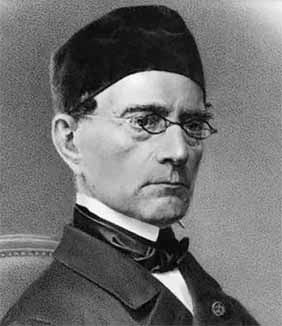
\includegraphics[scale=0.4]{img/lame}}
 \subcaptionbox{Cauchy\label{fig:Cauchy}}{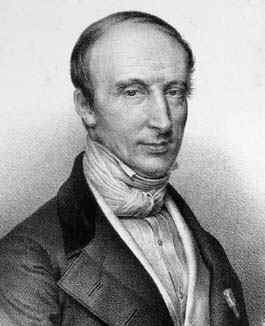
\includegraphics[scale=0.4]{img/Cauchy}}
 \caption{Lamé and Cauchy}
\end{figure}

In the doubting sight of the audience, Lamé enthusiastically told the Academy that he could not claim the entire credit for himself because the idea had been suggested to him in a casual conversation by his colleague Liouville (\cref{fig:Liouville}) some month before. Liouville took the floor after Lamé finished his presentation. He expressed some doubts on the proposed proof, and declined any credit for himself in the idea of introducing complex numbers, pointing out that many others, among them Euler, Lagrange, Gauss, Cauchy, and \enquote{above all Jacobi,} had used complex numbers in similar way in the past. Liouville said it was common that many mathematician came to the first idea of such, but the key point in this idea, whether an integer could be \emph{unique} factorized, though was true for integers, but lacked of evidence showing it could be extended to complex numbers.

Cauchy (\cref{fig:Cauchy}), who took the floor after Liouville, seemed to believe there was some likelihood that Lamé would succeed, because he, in turn, said he himself had presented to Academy in October 1846 an idea which he believed might yield a proof of Fermat's Last Theorem, but he had not found the time to develop it further. This sounded like a competition to Lamé: to see who can complete the proof first. In the following weeks, Lamé and Cauchy had a great deal of activity in pursuing these ideas. Lamé admitted the logical validity of Liouville's criticism, but he did not in the least share Liouville's doubts about the truth of the final conclusion. He showed \enquote{all his examples confirmed the existence of unique factorization for complex numbers.} and planned to prove this \enquote{lemma}. In the meeting of March 15th, Wantzel\footnote{Wantzel proved Gauss-Wantzel theorem, which solved geometric construction of regular polygons, and showed the insoluble of trisecting angle and doubling cube.} claimed to have \enquote{proved} the validity of unique factorization into primes, but his arguments covered only the case $n \leq 4$, then simply said that \enquote{one easily sees} that the same arguments can be applied to the case $n > 4$. However, others including Cauchy did not think so. Cauchy then launched into a long series of papers in which he himself attempt to prove a division algorithm for the complex numbers in question, from which he could conclude the validity of unique factorization.

In March 22nd, the competing reached its climax. Both Lamé and Cauchy deposited \enquote{secrete packets} with the Academy. The depositing of secrete packets was an institution of the Academy which allowed members to go on record as having been in possession of certain ideas at a certain time -- without revealing them -- in case a priority dispute later developed. This was definitely a good lessons learned from the priority dispute between Newton and Leibniz about Calculus. Lamé and Cauchy each published notices in the proceedings of the Academy; the problem was always \enquote{almost} done, but with some \enquote{minor} issue. Then, on May 24th, Liouville read into proceedings a letter from Kummer (\cref{fig:Kummer}) in Breslau which ended the entire discussion. Kummer confirmed that Liouville's doubts was correct. He not only asserted that unique factorization \emph{fails}, but also included with his letter a copy of a memoir he had published three years earlier in which he had demonstrated the failure of unique factorization. This ended the competition between Lamḿe and Cauchy.

\begin{figure}[htbp]
 \centering
 \subcaptionbox{Kummer \label{fig:Kummer}}{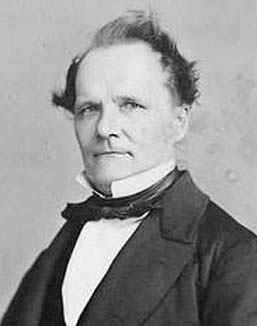
\includegraphics[scale=0.4]{img/Kummer}}
 \subcaptionbox{Liouville \label{fig:Liouville}}{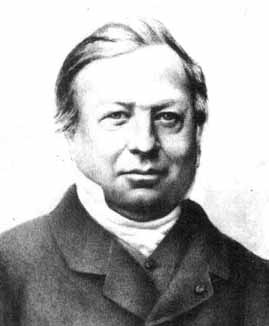
\includegraphics[scale=0.4]{img/liouville}}
 \caption{Kummer and Liouville}
\end{figure}

\index{ideal numbers} \index{Bernoulli numbers} \index{regular prime numbers}
But, the dramatic story was always with but, Kummer said the unique factorization could be \enquote{saved} by introducing a new kind of complex numbers which he called \enquote{ideal complex numbers} (or just ideal numbers) these results he had published one year earlier in the proceedings of the Berlin Academy and a complete exposition of them was soon to appear in Crelle's Journal. The ideal numbers could be used to proof Fermat's Last Theorem, and he had successfully in reducing its proof for a given $n$ to the testing of two conditions. But, another but, for some very strange prime numbers, for example 37, even ideal numbers don't exist. Kummer successfully proved Fermat's Last Theorem for all prime numbers within 100 except for 37, 59, and 69, that is, there is no solution for $x^p + y^p = z^p$ in integers\footnote{Kummer proved for any odd prime number $p$, if does not divide the nominator of any Bernoulli numbers of $B_2, B_4, \dotsc, B_{p-3}$, the Fermat's Last Theorem is true for $p$. Such prime numbers are called regular prime numbers. Where Bernoulli's numbers can be defined recursively as this: $B_0 = 1$, for any positive integer $n$ satisfying $\displaystyle \sum_{k = 0}^{n}\binom{n + 1}{k} B_k = 0$}. This was not only the best result before Andrew Wiles, but also initialized a new mathematical branch -- algebraic number theory.

\index{Kummer}
\begin{mdframed}
Ernst Eduard Kummer  (1810 - 1893) was a German mathematician. His faster, Carl Gotthelf Kummer, died when Eduard was only three years old. Eduard and his elder brother were brought up by their mother. In 1828 Kummer entered the University of Halle with the intention of studying Protestant theology. Fortunately, Kummer received mathematics teaching as part of his degree, designed to provide a proper foundation to the study of philosophy. Kummer's mathematical teacher, Scherk, inspired his interest in mathematics and Kummer soon was studying mathematics as his main subject. In 1831 Kummer was awarded a prize for a mathematical essay he wrote on a topic set by Scherk. He was soon awarded his certificate of teaching in schools and a doctorate. Kummer then taught a probation year from 1831 at the Gymnasium in Sorau where he had been educated. Then he had been teaching at the Gymnasium in Liegnitz, now Legnica in Poland over ten years. He taught mathematics and physics and sometimes other topics. His pupils were very fortunate to find a school teacher of Kummer's quality and ability to inspire. His two most famous pupils were Kronecker and Joachimsthal and, under Kummer's guidance, they were undertaking mathematical research while at school. Kummer did research while teaching. He published a paper on hypergeometric series in Crelle's Journal in 1836 and sent a copy to Jacobi. Jacobi and later Dirichlet, through the correspondence with Kummer, soon realised the great potential for the highest level of mathematics that Kummer possessed. In 1839, although still a school teacher, Kummer was elected to the Berlin Academy on Dirichlet's recommendation. Jacobi was about to find Kummer a university professorship.

In 1840 Kummer married a cousin of Dirichlet's wife. But sadly, his wife died in 1848. Despite this, Kummer made great achievement during these 8 years. In 1842, he was appointed a full professor at the University of Breslau, now Wrocław in Poland, under the strong support from Jacobi and Dirichlet. There he quickly established himself as an outstanding university teacher of mathematics and began to research number theory. In 1855 Dirichlet left Berlin to succeed Gauss at Göttingen. He recommended Kummer as his successor to Berlin, which indeed they did. While accepted, Kummer wanted Weierstrass as his colleague, yet he realised that Weierstrass was a strong candidate for the chair he was leaving vacant in Breslau. Kummer then recommended his former student Joachimsthal to Breslau. As the result, in 1856 Weierstrass came to Berlin as Kummer wanted. Further, Kronecker joined in 1855. Berlin became one of the leading mathematical centres in the world. In 1861 Kummer and Weierstrass established Germany's first pure mathematics seminar in Berlin. He became the most popular professors to the students. \enquote{Kummer's popularity as a professor was based mot only on the clarity of his lectures but on his charm and sense of humour as well. Moreover, he was concerned for the well-being of his students and willingly aided them when material difficulties arose...} wrote by his student.

During Kummer's first period of mathematics he worked on function theory and differential equations. In 1843, when attempting to prove Fermat's Last Theorem, Kummer realized the unique factorization did not extend to complex numbers. To restore the uniqueness of factorization, he introduced \enquote{ideal} numbers. Not only has his work been most fundamental to Fermat's Last Theorem, since all later work was based on it for many years, but the concept of an ideal numbers led to the development of ring theory and much of abstract algebra. The Paris Academy of Sciences awarded Kummer the Grand Prize in 1857 for this work. In fact the prize of 3,000 francs was offered for a solution to Fermat's Last Theorem but when no solution was forthcoming, even after extending the date (unless extended for 138 years), the Prize was given to Kummer even though he had not submitted an entry for the Prize. Soon after Kummer was awarded the Grand Prix he was elected to membership of the Paris Academy of Sciences and then, in 1863, he was elected a Fellow of the Royal Society of London.

Starting from a school teacher, Kummer ended up with high office in the Academy. He was secretary of the Mathematics/Physics Section of the Academy from 1863 to 1878. He also held high office in the University of Berlin, being Dean in 1857 - 1858 and again in 1865 - 1866. He was rector of the university in 1868 - 1869. Kummer supervised a large number of doctoral students, including Bachmann, Cantor, du Bois-Reymond, Gordan, Schönflies and Schwarz. In fact Schwarz became related to Kummer when he married one of his daughters. Fuchs succeeded Kummer after he retired in 1883.
\end{mdframed}

\section{Gaussian integers}

\index{algebraic numbers}
In order to extend concepts like divide, prime to complex numbers, we need define what is complex integer. An intuitive definition looks like $a + bi$ for integers $a$ and $b$. However, Euler seemed to treat $a + i\sqrt{3}b$ as \enquote{integers}. Historically, people discovered new numbers through equations: through linear equation $ax = b$, recognized rational numbers as $x = \dfrac{b}{a}$; through quadratic equations, recognized irrational numbers; through cubic equations, recognized complex numbers; through higher degree equations, recognized numbers that can't be expressed in radicals; these numbers, by the fundamental theorem of algebra, are complex numbers defined by algebraic equation:

\[
a_n x^n + a_{n-1} x^{n-1} + \dotsb + a_1 x + a_0 = 0
\]

\index{transcendent numbers}
where $a_n, a_{n-1}, ..., a_1, a_0$ are integers. Why needn't these coefficients be rational? Suppose they are, that is, $a_i = \dfrac{b_i}{c_i}$; multiply both sides by the least common multiple of the denominators, consequently, the coefficients change back to integers. Thereby, it's sufficient to assume the coefficients be integers, Hermite in 1873 showed $e$ was not a solution to any of such algebraic equations and Lindemann in 1882 showed $\pi$ was not a solution to any algebraic equations too. We call the numbers that satisfy some algebraic equation algebraic numbers, otherwise, transcendent numbers, therefore, $\pi, e$ are transcendent numbers. Algebraic numbers can be abstract, indirect. Different from numbers like $1 + i\sqrt{2}$, there is no uniformed general expression for algebraic numbers; they are roots to some algebraic equations, but may not be expressed in radicals. By this definition, when $n = 1$, the solution to linear equation $ax + b = 0$ is $x = \dfrac{b}{a}$. If the coefficient $a = 1$, then $x$ is integral; inspired by this, we define when $a_n = 1$, a solution to the algebraic equation:

\index{algebraic integers}
\[
x^n + a_{n-1} x^{n-1} + \dotsb + a_1 x + a_0 = 0
\]

\index{monic equation} \index{Gaussian integers} \index{rational integers}
is an \emph{algebraic integer}, such equation is called \emph{monic} equation. Algebraic integers include both normal integers (also named \emph{rational} integers, see \cref{qn:rational-solution-is-integral}) and those more complex ones. We may start from the simplest monic quadratic equations. When the coefficient to the linear term is even, like $x^2 - 2ax + a^2 + b^2 = 0$, its solution is $a \pm bi$. Gauss was the first studied this kind of numbers; we call them Gaussian integers, denoted by $\mathbb{Z}[i]$. This notation indicates that we adjoin\footnote{The notation $\mathbb{Z}[x]$ is called the polynomials in the ring of integers $\mathbb{Z}$, it contains polynomials in the form of $a_n x^n + a_{n-1} x^{n-1} + \dotsb + a_1 x + a_0$, where the coefficients $a_0, a_1, \dotsc, a_n \in \mathbb{Z}$ are integers.} the irrational number $i$ to integers $\mathbb{Z}$.

To distinguish algebraic integers from normal, rational integers, we use Greek letters $\alpha, \beta, \gamma, \dotsc$ for algebraic integers (see \cref{ch:greek-letters} for the Greek alphabetic table), use English letters $a, b, c, \dotsc$ for rational integers. Analogous to rational integers, it's easy to verify that the results of $+, -, \times$ between Gaussian integers are still Gaussian integers, but division is not (this is as same as the result of division between normal rational integers may not necessarily be rational integers). It's necessary to define the concept of divide: if a Gaussian integer $\alpha = \beta\gamma$ is the product of two Gaussian integers, then $\beta$ divides $\alpha$. The next two problems are a bit complex: (1) How to define the division algorithm (in terms of quotient and remainder) ? (2) How to define Gaussian prime numbers?

\index{norm}
The division algorithm involves the concept of \enquote{less than}. Remind the division algorithm for rational integers, namely $a = bq + r$, where $r < b$. It demands the remainder to be \enquote{less than} $b$. However, complex numbers are essentially vectors, which can't be compared directly. We can't say $1 + i$ is \enquote{less than} 2. Only the modulus can be compared, for example, $|1 + i| = \sqrt{1^2 + 1^2} = \sqrt{2} < 2 = |2|$. To make the meaning of \enquote{less than} valid, Gauss in 1832 introduced an important concept: norm. The norm of a complex integer $z = a + bi$ is defined as:

\[
N(z) = a^2 + b^2
\]

It equals the square of modulus, hence is always $\geq 0$. It also closely relates to conjugates:

\[
N(z) = a^2 + b^2 = z\overline{z} = N(\overline{z})
\]

Same as the modulus, norm is multiplicative (see \cref{qn:norm-is-multiplicative}):

\[
N(\alpha\beta) = N(\alpha)N(\beta)
\]

\index{Gaussian integers!units} \index{Gaussian integers!associates}
With the concept of norm, Gauss extended the notion of 1. For normal rational integers, $3 = 3 \times 1$. Things get complicated when considering negative integers: $-3 = 3 \times (-1) = -3 \times 1$, but when taking absolute value, it unifies to $|3| = |(\pm 3) \times (\pm 1)| = 3 \times 1$. Gauss defined a number was a \emph{unit} if its norm $N(\mu) = 1$; if $\alpha = \mu \alpha'$, then call $\alpha'$ is an associate of $\alpha$. In above example of rational integers, $-1, 1$ are units, and $-3$ is an associate of 3. Extending to Gaussian integers, there are four units: $\pm 1, \pm i$. For example, $1 + i = (1 - i)i$, since $|i| = 1$ is a unit, $1 + i$ is associate of $1 - i$, which is analogous to rational integers $\pm 3$. A unit can be equivalently defined as the number that divides 1. It follows that $\mu^n = 1$ and interestingly, the two units of rational integers are $(-1)^0, (-1)^1$; and the four units of Gaussian integers are $i^{0, 1, 2, 3}$. Don't you remind the cyclotomic equations?

The concept of norm allows us to define division algorithm. An intuitive idea is to replace $r < b$ of rational integers with $N(\gamma) < N(\beta)$ of Gaussian integers, such that the division algorithm could be defined as,

\begin{align*}
\alpha &= \rho \beta + \gamma & \text{其中} \beta &\ne 0, N(\gamma) < N(\beta)
\end{align*}

But hold on. Given $\alpha$ and $\beta$, do the quotient $\rho$ and the remainder $\gamma$ necessarily exist? If no, then this definition would be invalid. Gauss showed:

\index{Gaussian integers!division algorithm}
\begin{theorem}
Given Gaussian integers $\alpha$ and $\beta \ne 0$, there are Gaussian integers $\rho, \gamma$ such that $\alpha = \rho \beta + \gamma$, where $N(\gamma) < N(\beta)$.
\end{theorem}

\begin{proof}
Let $\rho = m + ni$, where $m, n$ are rational integers. All the products of $\rho \beta$ are in the form of,

\[
\rho \beta = (m + ni)\beta = m\beta + ni\beta
\]

It is the sum of some multiple of $\beta$ and some multiple of $i\beta$. The geometric interpretation of $i\beta$ is to turn the vector $\beta$ by 90 degrees (see \cref{qn:mul-i}). As shown in \cref{fig:zi}, $i\beta$ is perpendicular to $\beta$. It turns out all $\rho \beta$ are grids of squared lattice with side length of $|\beta|$.

\begin{figure}[htbp]
 \centering
 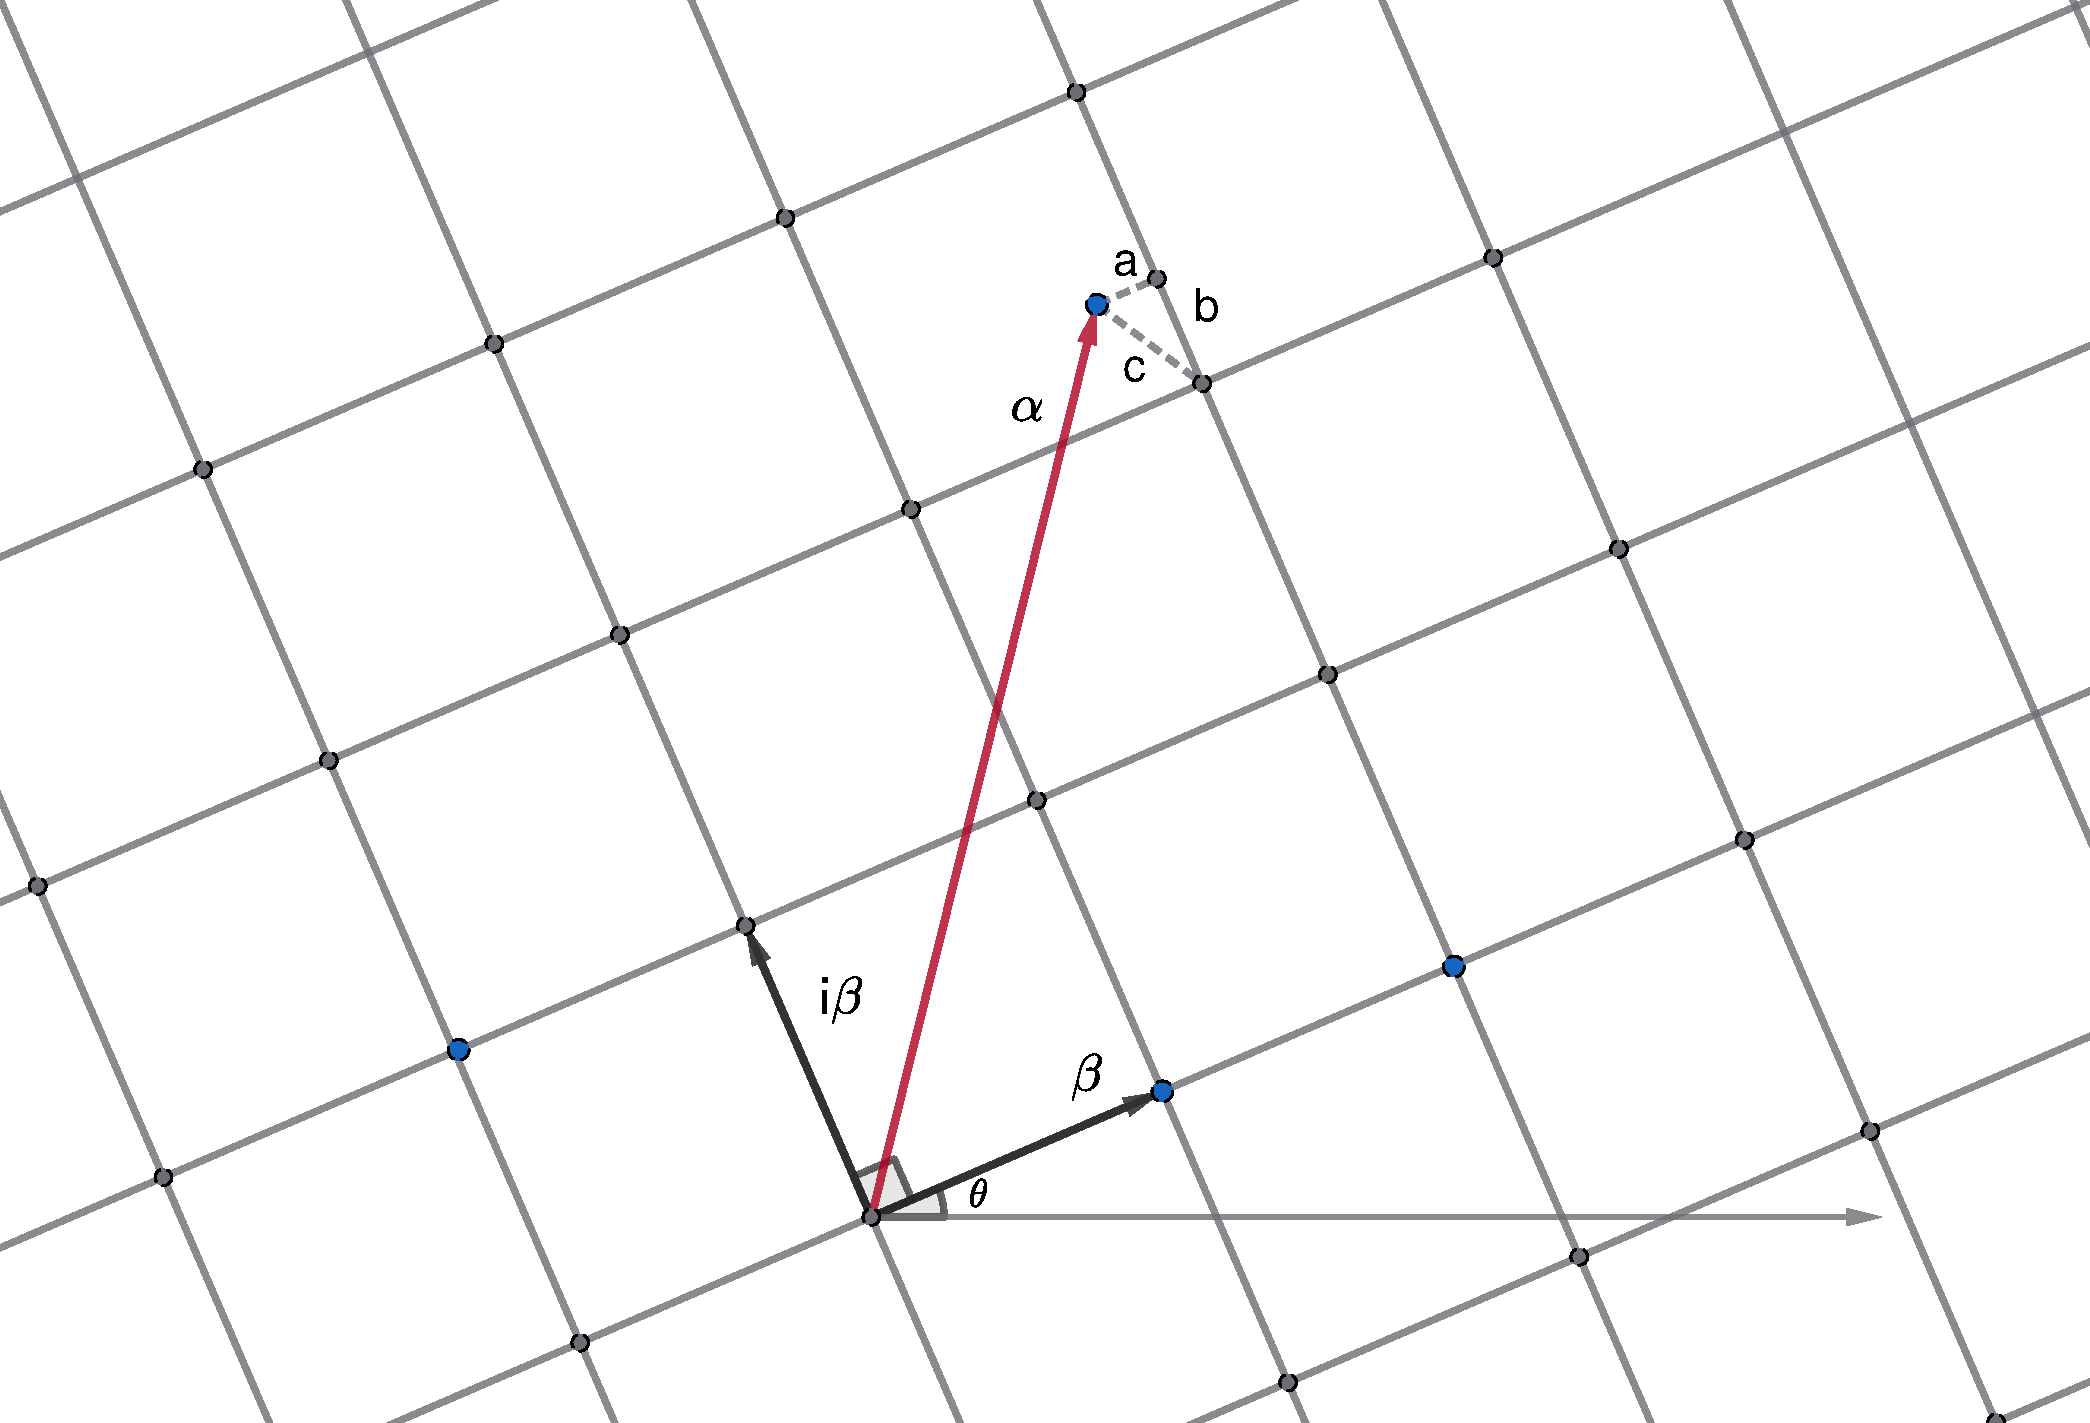
\includegraphics[scale=0.3]{img/zi}
 \caption{Gaussian integers $\rho \beta$ form a lattice, number $\alpha$ lies in some square (include boundaries).}
 \label{fig:zi}
\end{figure}

The number $\alpha$ lies in some square (include boundaries). The distance from it to either nearest sides is $\leq \frac{|\beta|}{2}$ (as shown in \cref{fig:zi}, $a, b \leq \frac{|\beta|}{2}$). For any triangle, the length of two sides is longer than the third, therefore,

\[
|\gamma| = |c| < |a| + |b| \leq \frac{|\beta|}{2} + \frac{|\beta|}{2} = |\beta|
\]
Taking square on both sides gives $N(\gamma) < N(\beta)$.
\end{proof}

\index{Gaussian integers!Euclidean algorithm}
The existence of division algorithm implies Euclidean algorithm (see \cref{sec:Euclidean-algorithm}). Gauss extended the Euclidean algorithm to Gaussian integers.

\begin{align*}
\alpha   &= \rho_1 \beta + \gamma_1    & N(\gamma_1) &< N(\beta) \\
\beta    &= \rho_2 \gamma_1 + \gamma_2 & N(\gamma_2) &< N(\gamma_1) \\
\gamma_1 &= \rho_3 \gamma_2 + \gamma_3 & N(\gamma_3) &< N(\gamma_2) \\
         & \dotso
\end{align*}

This process can not be endless. Since norm is non-negative, there is some $n$ such that $N(\beta) > N(\gamma_1) > N(\gamma_2) > \dotsb > N(\gamma_n) > N(\gamma_{n+1})= 0$, in other words,

\begin{align*}
\gamma_{n-2} &= \rho_n \gamma_{n-1} + \gamma_n & N(\gamma_n) &< N(\gamma_{n-1}) \\
\gamma_{n-1} &= \rho_{n+1} \gamma_n && \text{no remainder}
\end{align*}

Consequently, $\gamma_n$ divides $\gamma_{n-1} \to$ divides $\gamma_{n-2} \to \dotsb \to$ divides $\beta \to$ divides $\alpha$, therefore, $\gamma_n$ is a common divisor of $\alpha, \beta$. Conversely, any common divisor $\psi$ of $\alpha, \beta$ divides $\alpha \to$ divides $\beta \to$ divides $\gamma_1 \to$ divides $\gamma_2 \to \dotsb \to$ divides $\gamma_n$. It follows that $\gamma_n = (\alpha, \beta)$ is a \emph{highest} common divisor \footnote{It is \emph{highest}, but not \emph{greatest}, because we can not directly compare complex numbers.}. We use the term \emph{a highest} because: (1) We can not compare complex numbers directly for their magnitudes; the term \enquote{highest} means any common divisor $\psi$ divides $\gamma_n$. (2) Highest common divisor is not unique, because if a number multiplied by a unit $\mu\phi = \gamma_n$, then $\phi$ is also a highest common divisor. For example, A highest common divisor of $3 + i$ and $1 + 3i$ is $-1 + i$, multiplying it by $-1, \pm i$ gives associates $1 - i, i(-1 + i) = -1 - i, -i(-1 + i) = 1 + i$, which are all highest common divisors.

Gauss next defined what were Gaussian primes. Once extending to complex numbers, among those rational primes $2, 3, 5, 7, \dotsc$, some can be factorized, for example, $2 = (1 + i)(1 - i), 5 = (2 + i)(2 - i)$. Intuitively speaking, prime numbers are the \enquote{building blocks}, which should not be further factorized. But what does the term \enquote{further} mean? For example, $1 + i = (1 - i)i$. This is exactly why Gauss introduced the concept unit and associate. If a number can only be factorized by its associates and units, it is by no means of \enquote{further}. Gauss thus defined Gaussian prime as below.

\index{Gaussian integers!prime}
\begin{definition}
A Gaussian integer is prime if it is not 0 or any unit, and can only be divided by its associates and units.
\end{definition}

\index{Gaussian prime} \index{rational prime}
To differentiate from the normal prime numbers, we call such defined numbers \emph{Gaussian prime}, and the normal ones \emph{rational prime}. We use English letter $p$ for rational prime numbers, and Greek letter $\pi$ for Gaussian prime numbers. Definitely it has nothing to do with circles. After extending to Gaussian integers, a prime number $\pi$ has 8 factors: $\pm 1, \pm i, \pm \pi, \pm i\pi$. The next problem is how to find Gaussian primes?

\begin{proposition}\label{thm:prime-norm}
If the norm of a Gaussian integer $\psi$ is some rational prime number $p$, then $\psi$ is a Gaussian prime number.
\end{proposition}

\begin{proof}
Suppose $\psi = \alpha\beta$, a product of two Gaussian integers. Taking norm of both sides:

\begin{align*}
p &= N(\psi) = N(\alpha\beta) = N(\alpha)N(\beta)  && \text{norm is multiplicative}
\end{align*}

Since a rational prime number has only two rational factors of $1, p$, it implies either $N(\alpha)$ or $N(\beta)$ is 1, in other words, a unit. The other is an associate of $\psi$. Therefore, $\psi$ is Gaussian prime by definition.
\end{proof}

Using this proposition, we immediately knows $1 \pm i, 2 \pm i, 1 \pm 2i$ are all Gaussian prime numbers (Their norms: $N(1 \pm i) = 1^2 + 1^2 = 2, N(2 \pm i) = N(1 \pm 2i) = 1^2 + 2^2 = 5$ are all rational prime numbers). However, the converse of this proposition is not true, in other words, the norm of a Gaussian prime number may not be rational prime. For example, $N(3) = 9$ isn't rational prime, but suppose 3 can be factored into two Gaussian integers $3 = (a + bi)(c + di)$. Take norm of both sides:

\[
9 = N(3) = N(a + bi)N(c + di) = (a^2 + b^2)(c^2 + d^2)
\]

It's easy to verify that 3 is not a sum of two squares (3 can be only decomposed to 3 = 2 + 1, where 2 is not a square), hence it's impossible to have $a^2 + b^2 = c^2 + d^2 = 3$. It turns out that $a^2 + b^2$ and $c^2 + d^2$ can only be 1 or 9. Either one with the norm of 1 is a unit of Gaussian integers. Therefore, 3 is Gaussian prime by definition. It also reveals the fact that if a rational prime $p$ is a sum of two squares $p = a^2 + b^2$, then it can be factorized as $p = (a + bi)(a - bi)$, hence is not Gaussian prime; otherwise, if $p$ isn't any sum of two squares, apply the similar argument, suppose $p = (a + bi)(c + di)$ and take norms:

\[
p^2 = N(p) = N(a + bi)N(c + di) = (a^2 + b^2)(c^2 + d^2)
\]

Since $p$ is not any sum of two squares, it's impossible to have $a^2 + b^2 = c^2 + d^2 = p$; It turns out that $a^2 + b^2$ and $c^2 + d^2$ can only be 1 or $p^2$. Either one with the norm of 1 is a unit of Gaussian integers. Therefore, $p$ is Gaussian prime. Among the rational prime numbers, only 2 is even. As $2 = 1^2 + 1^2$, hence $2 = (1 + i)(1 - i)$ is not Gaussian prime. We've known that $1 \pm i$ and its associates are Gaussian prime. The remaining odd rational prime numbers fall into two classes: those in $4n + 3$ and in $4n + 1$. As 3 is in the first class, one may guess rational prime numbers in $4n + 3$ are not any sum of two squares. Fortunately, it's true.

\index{sum of two squares}
\begin{proposition}
The odd prime numbers in $4n + 3$ can not be represented as the sum of two squares.
\end{proposition}

\begin{proof}
Assume for contradiction that $a^2 + b^2 = 4n + 3$ for some integers $a$ and $b$. we claim that the parity of $a, b$ are different otherwise the sum of their squares would be even. Suppose $a = 2k + 1, b = 2m$, substitute in:

\[
a^2 + b^2 = (2k + 1)^2 + (2m)^2 = 4k^2 + 4k + 1 + 4m^2 = 4(k^2 + k + m^2) + 1
\]

Which is in $4n + 1$ but not $4n + 3$, a contradiction.
\end{proof}

It immediately follows that $3, 7, 11, \dotsc$ are Gaussian prime numbers. To deal with rational prime numbers in $4n + 1$, we need a tool, namely the fundamental theorem of arithmetic for Gaussian integers. The idea is as same as in \cref{sec:fundamental-theorem-of-arithmetic}, to derive the fundamental theorem from the Euclidean algorithm for Gaussian integers.

\begin{proposition}
If two Gaussian integers $\alpha, \beta$ are relatively prime, that is, $(\alpha, \beta) = 1$, and $\alpha$ divides $\beta \psi$, then $\alpha$ divides $\psi$.
\end{proposition}

\begin{proof}
Multiplying all numbers in the normal Euclidean algorithm by $\psi$, the last step is,

\begin{align*}
(\alpha \psi, \beta \psi) &= \gamma_n \psi = \psi  && \text{by } 1 = (\alpha, \beta) = \gamma_n
\end{align*}

Therefore, the highest common divisor is $\psi$. If $\alpha$ divides $\beta \psi$, since $\alpha$ also divides $\alpha \psi$, then $\alpha$ is a common divisor, which divides the highest common divisor $\psi$.
\end{proof}

\begin{corollary}\label{thm:Gaussian-primary}
If a Gaussian prime number $\pi$ divides $\alpha \beta$, then $\pi$ divides $\alpha$ or $\pi$ divides $\beta$.
\end{corollary}

\begin{proof}
Suppose $\pi$ does not divide $\alpha$, then $(\pi, \alpha) = 1$. since $\pi$ divides $\alpha \beta$, by above proposition, $\pi$ divides $\beta$.
\end{proof}

This corollary leads to the fundamental theorem of arithmetic for Gaussian integers.

\index{Gaussian integers!fundamental theorem of arithmetic}
\begin{theorem}[Fundamental theorem of arithmetic for Gaussian integers]
Every nonzero Gaussian integer can be represented as the product of Gaussian prime numbers \emph{uniquely} up to order, associates, and units.
\end{theorem}

\begin{proof}
Assume for contradiction that there is some Gaussian integer has two distinct factorization:

\[
\pi_1 \pi_2 \dotsm \pi_j = \psi_1 \psi_2 \dotsm \psi_k
\]

Suppose some prime factor $\pi_i$ is not a unit, nor associate of any prime factor on the right side. By above corollary, since the prime number $\pi_i$ divides the product of relatively prime factors, namely $\psi_1 \psi_2 \dotsm \psi_k$, it follows that $\pi_i$ divides $\psi_1$, or $\psi_2, \dotsc, $ or $\psi_k$. But it's impossible because every prime number $\psi_1, \psi_2, \dotsc, \psi_k$ can not be divided by any non-associate. Therefore, every Gaussian integer has a unique factorization up to order, associates, and units.
\end{proof}

\index{Wilson's theorem}
Now we are ready to deal with the rational prime numbers in $4n + 1$, thus completely classify Gaussian primes. We need Wilson's theorem in elementary number theory (see \cref{app:wilsons-theorem}): if $p$ is a prime number, then the factorial $(p - 1)! \equiv -1 \pmod p$.

\begin{lemma}
There is some sum of squares in $x^2 + 1$ that can be divided by rational prime number in $p = 4n + 1$.
\end{lemma}

\begin{proof}
As $p = 4n + 1$, the factorial $(p - 1)!$ consists of $4n = 2n + 2n$ terms:
\begin{align*}
(p - 1)! &= 1 \cdot 2  \dotsm  2n \cdot (2n + 1)  \dotsm  4n \\
  &= (1 \cdot 2  \dotsm  2n)[(p - 1) \cdot (p - 2)  \dotsm  (p - 2n)] && \text{reverse the second half} \\
  &\equiv (1 \cdot 2  \dotsm 2n)(-1 \cdot -2 \dotsm -2n) \pmod p && \text{by } p - k \equiv k \pmod p \\
  &\equiv (2n)!(-1)^{2n}(2n)! = [(2n)!]^2 = x^2 \pmod p && \text{let } x = (2n)!
\end{align*}
On the other hand, by Wilson's theorem, $(p - 1)! \equiv -1 \pmod p$, therefore, $x^2 \equiv -1 \pmod p$, that is, $p$ divides some $x^2 + 1$.
\end{proof}

Now rational prime number $p = 4n + 1$ divides some $x^2 + 1 = (x + i)(x - i)$. If $p$ is also a Gaussian prime number, then $p$ divides $x + i$ or $x - i$ (by corollary \ref{thm:Gaussian-primary}). But $\dfrac{x}{p} \pm \dfrac{1}{p}i$ cannot be Gaussian integer, a contradiction. It turns out that $p$ cannot be Gaussian prime, hence can be factorized as $p = (a + bi)(c + di)$, where $a + bi$ and $c + di$ are not both units ($a^2 + b^2 \ne 1 \ne c^2 + d^2$). Take norm of both sides:

\[
p^2 = N(p) = N(a+bi)N(c+di) = (a^2 + b^2)(c^2 + d^2)
\]

It can only be $a^2 + b^2 = c^2 + d^2 = p$. On the other hand, if $p = a^2 + b^2 = (a + bi)(a - bi)$, since $N(a \pm bi) = p$ and by proposition \ref{thm:prime-norm}, they are both Gaussian prime numbers. Further by fundamental theorem of arithmetic for Gaussian integers, the factorization is \emph{unique}, therefore, $a^2 = c^2, b^2 = d^2$. This settles down the case of $4n + 1$, and with Gaussian integers, one may prove below result\footnote{In a letter to Mersenne on 25th December 1640, Fermat gave this proposition. Fermat told his friends multiple times that he had proved it by infinite descent, but no document suggest this. About a century later, Euler in 1754 proved this proposition for the first time.}:

\index{Fermat's theorem of sum of squares}
\begin{theorem}[Fermat's theorem of sum of squares]
Every rational number in $p = 4n + 1$ can be represented as the sum of two squares $a^2 + b^2$.
\end{theorem}

To classify all Gaussian prime numbers, there are cases in terms of rational prime numbers: (1) The only even prime number $p = 2$; (2) odd prime numbers in $4n + 3$; (3) old prime numbers in $4n + 1$.

\begin{theorem}
There are three types of Gaussian prime number: (1) $1 + i$ and its associates; (2) The rational prime numbers in $4n + 3$ and their associates; (3) the factor $a + bi$ of rational prime numbers in $4n + 1$.
\end{theorem}

\index{Gauss}
\begin{mdframed}
After discovered the regular 17-gon could be constructed by ruler and compass (see \cref{sec:Gauss-17-gon}), Gauss returned to Brunswick in 1799. He submitted his doctoral thesis on the Fundamental Theorem of Algebra to the University of Helmstedt and was awarded his doctorate. The Duke of Brunswick promised to continue funding him, allowing Gauss to devote himself entirely to mathematics and scientific research. In the summer of 1801, he published \emph{Disquisitiones Arithmeticae}, a famous work in number theory. On New Year’s Day 1801, the Italian astronomer Giuseppe Piazzi (1746–1826) discovered a new asteroid, Ceres. However, Piazzi had collected only a small amount of observational data before Ceres moved behind the Sun and disappeared from view. Gauss’s friend, the German astronomer Franz Xaver von Zach (1754–1832), informed Gauss of this situation. Gauss performed calculations — likely with the method of least squares — and predicted the orbit of Ceres in June. His prediction differed sharply from those of other astronomers. On December 7 that year, Zach observed Ceres again as it reappeared from behind the Sun, and its orbit matched Gauss’s prediction exactly. Gauss rose to fame overnight across European academia. Heinrich Wilhelm Olbers (1758–1840), an astronomer at the University of Göttingen, invited Gauss to become the director of the university’s newly built observatory.

%% https://www.liquisearch.com/carl_friedrich_gauss/family
While Gauss made great progress in his career, his personal life was a mess. In 1805, Gauss married Johanna Osthoff. The following year, the Duke of Brunswick, Gauss’s patron, served as a military commander and led the Prussian forces against Napoleon. He was wounded in defeat at the Battle of Jena and died the same year. His duchy was subsequently occupied by France (and restored after Napoleon’s defeat in 1813). This was a devastating blow to Gauss, who repeatedly stated that without the duke’s support, his academic career would never have been possible. In 1808, Gauss’s father died. Misfortune continued to strike: his wife Johanna died shortly after giving birth to their third child, and their son Louis died in infancy. Gauss never fully recovered from these losses. He later remarried to Minna Waldeck, with whom he had three more children. However, his second wife suffered from tuberculosis for many years. Gauss’s family life was unhappy: his ill wife troubled him greatly, and he sometimes vented his frustration on his children. His son Eugen left home in anger in 1830 and emigrated to the United States. His wife died the next year. From then on, his youngest daughter Therese cared for Gauss until his death.

%% https://www.britannica.com/biography/Carl-Friedrich-Gauss
Gauss's work never seemed suffer from his personal tragedy. In addition to astronomy, he devoted a great deal of time and effort to the geodetic survey of the Kingdom of Hanover from 1818 to 1825. During this work, Gauss invented the heliotrope — an instrument that concentrates sunlight into a beam visible several miles away — which significantly improved the precision of observations. From his geodetic work, Gauss developed the concept of curvature of surfaces, laying the theoretical foundation for the field of differential geometry. From manuscripts unpublished during his lifetime, it is clear that Gauss was also fully aware of non-Euclidean geometry. In the 1830s, Gauss experienced something of a rebirth with the arrival of the young physicist Wilhelm Eduard Weber (1804–1891) at the University of Göttingen. Gauss collaborated with Weber on geomagnetism and electromagnetism, and took part in the first global survey of the Earth’s magnetic field — for which he invented the magnetometer. Together, they built one of the earliest telegraph systems, capable of sending signals from the Göttingen Observatory to Weber’s office, although the invention was not further developed. From this work, Gauss developed potential theory, which became an important branch of mathematical physics. This collaboration did not last, however. In 1837, Weber was fired for his courageous refusal to swear an oath of allegiance to the new King of Hanover.

Gauss directed many talent students in his later years, including Eisenstein, Dedekind, and Riemann. Gauss might have been lonely, his ideas and genius surpassing those around him, yet he could see that these young mathematicians would take up the torch and carry his legacy forward.
\end{mdframed}

\section{Quadratic integers}
\index{quadratic integers} \index{quadratic numbers}
Gaussian integers correspond to the simplest case of monic quadratic equations. The solutions to the more generic equation, $x^2 - 2ax + (a^2 + mb^2) = 0$, are in the form of $a \pm b\sqrt{-m}$, where $m$ is square free. Because the algebraic integers in this form are solutions to quadratic equations, they are called \emph{quadratic integers}, or quadratic numbers, denoted by $\mathbb{Z}[\sqrt{-m}]$. For example, $\mathbb{Z}[\sqrt{-2}], \mathbb{Z}[\sqrt{-3}]$ and so on. The factorization Euler did when proving Fermat's Last Theorem for $n=3$,

\[
p^2 + 3q^2 = (p + q\sqrt{-3})(q - q\sqrt{-3})
\]

is about quadratic integers in $\mathbb{Z}[\sqrt{-3}]$. What Gauss did for $\mathbb{Z}[i]$ set a good example with these steps: (a) define norm, (b) if valid, extend Euclidean algorithm, (c) find out the primes. Let us apply them to $\mathbb{Z}[\sqrt{-2}]$. Inspired by conjugate complex numbers, we extend the definition of norm to,

\index{quadratic integers!norm}
\begin{definition}
The norm of quadratic integers $\xi = a + b\sqrt{-m}$ is $N(\xi) = \xi\overline{\xi} = (a + b\sqrt{-m})(a - b\sqrt{-m}) = a^2 + mb^2$.
\end{definition}

It is not by chance that the norm equals the constant term of the quadratic equation (see \cref{qn:quadratic-norm}). In $\mathbb{Z}[\sqrt{-2}]$, the norm is $a^2 + 2b^2$ and the units are $\mu = \pm 1$. We next check whether Euclidean algorithm is valid in $\mathbb{Z}[\sqrt{-2}]$, in other words, for any quadratic integers $\alpha, \beta \ne 0$, whether there are quadratic integers $\rho, \gamma$ satisfying $\alpha = \rho \beta + \gamma$, and $N(\gamma) < N(\beta)$. Let $\rho = m + n\sqrt{-2}$, then $\rho \beta = m\beta + n\sqrt{-2}\beta$ is a lattice of rectangles spanned by vectors $\beta$ and $i\sqrt{2}\beta$, as shown in \cref{fig:Z-sqrt-2}. Since $i\sqrt{2}\beta$ is obtained by rotating $\beta$ by 90 degree, followed by scaling up $\sqrt{2}$ times, the width of the rectangle is $|\beta|$ and the length is $\sqrt{2}|\beta|$. Any quadratic integer $\alpha$ lies in some rectangle, hence the square of its distance to the closest corner, by Pythagorean theorem, is,

\begin{figure}[htbp]
 \centering
 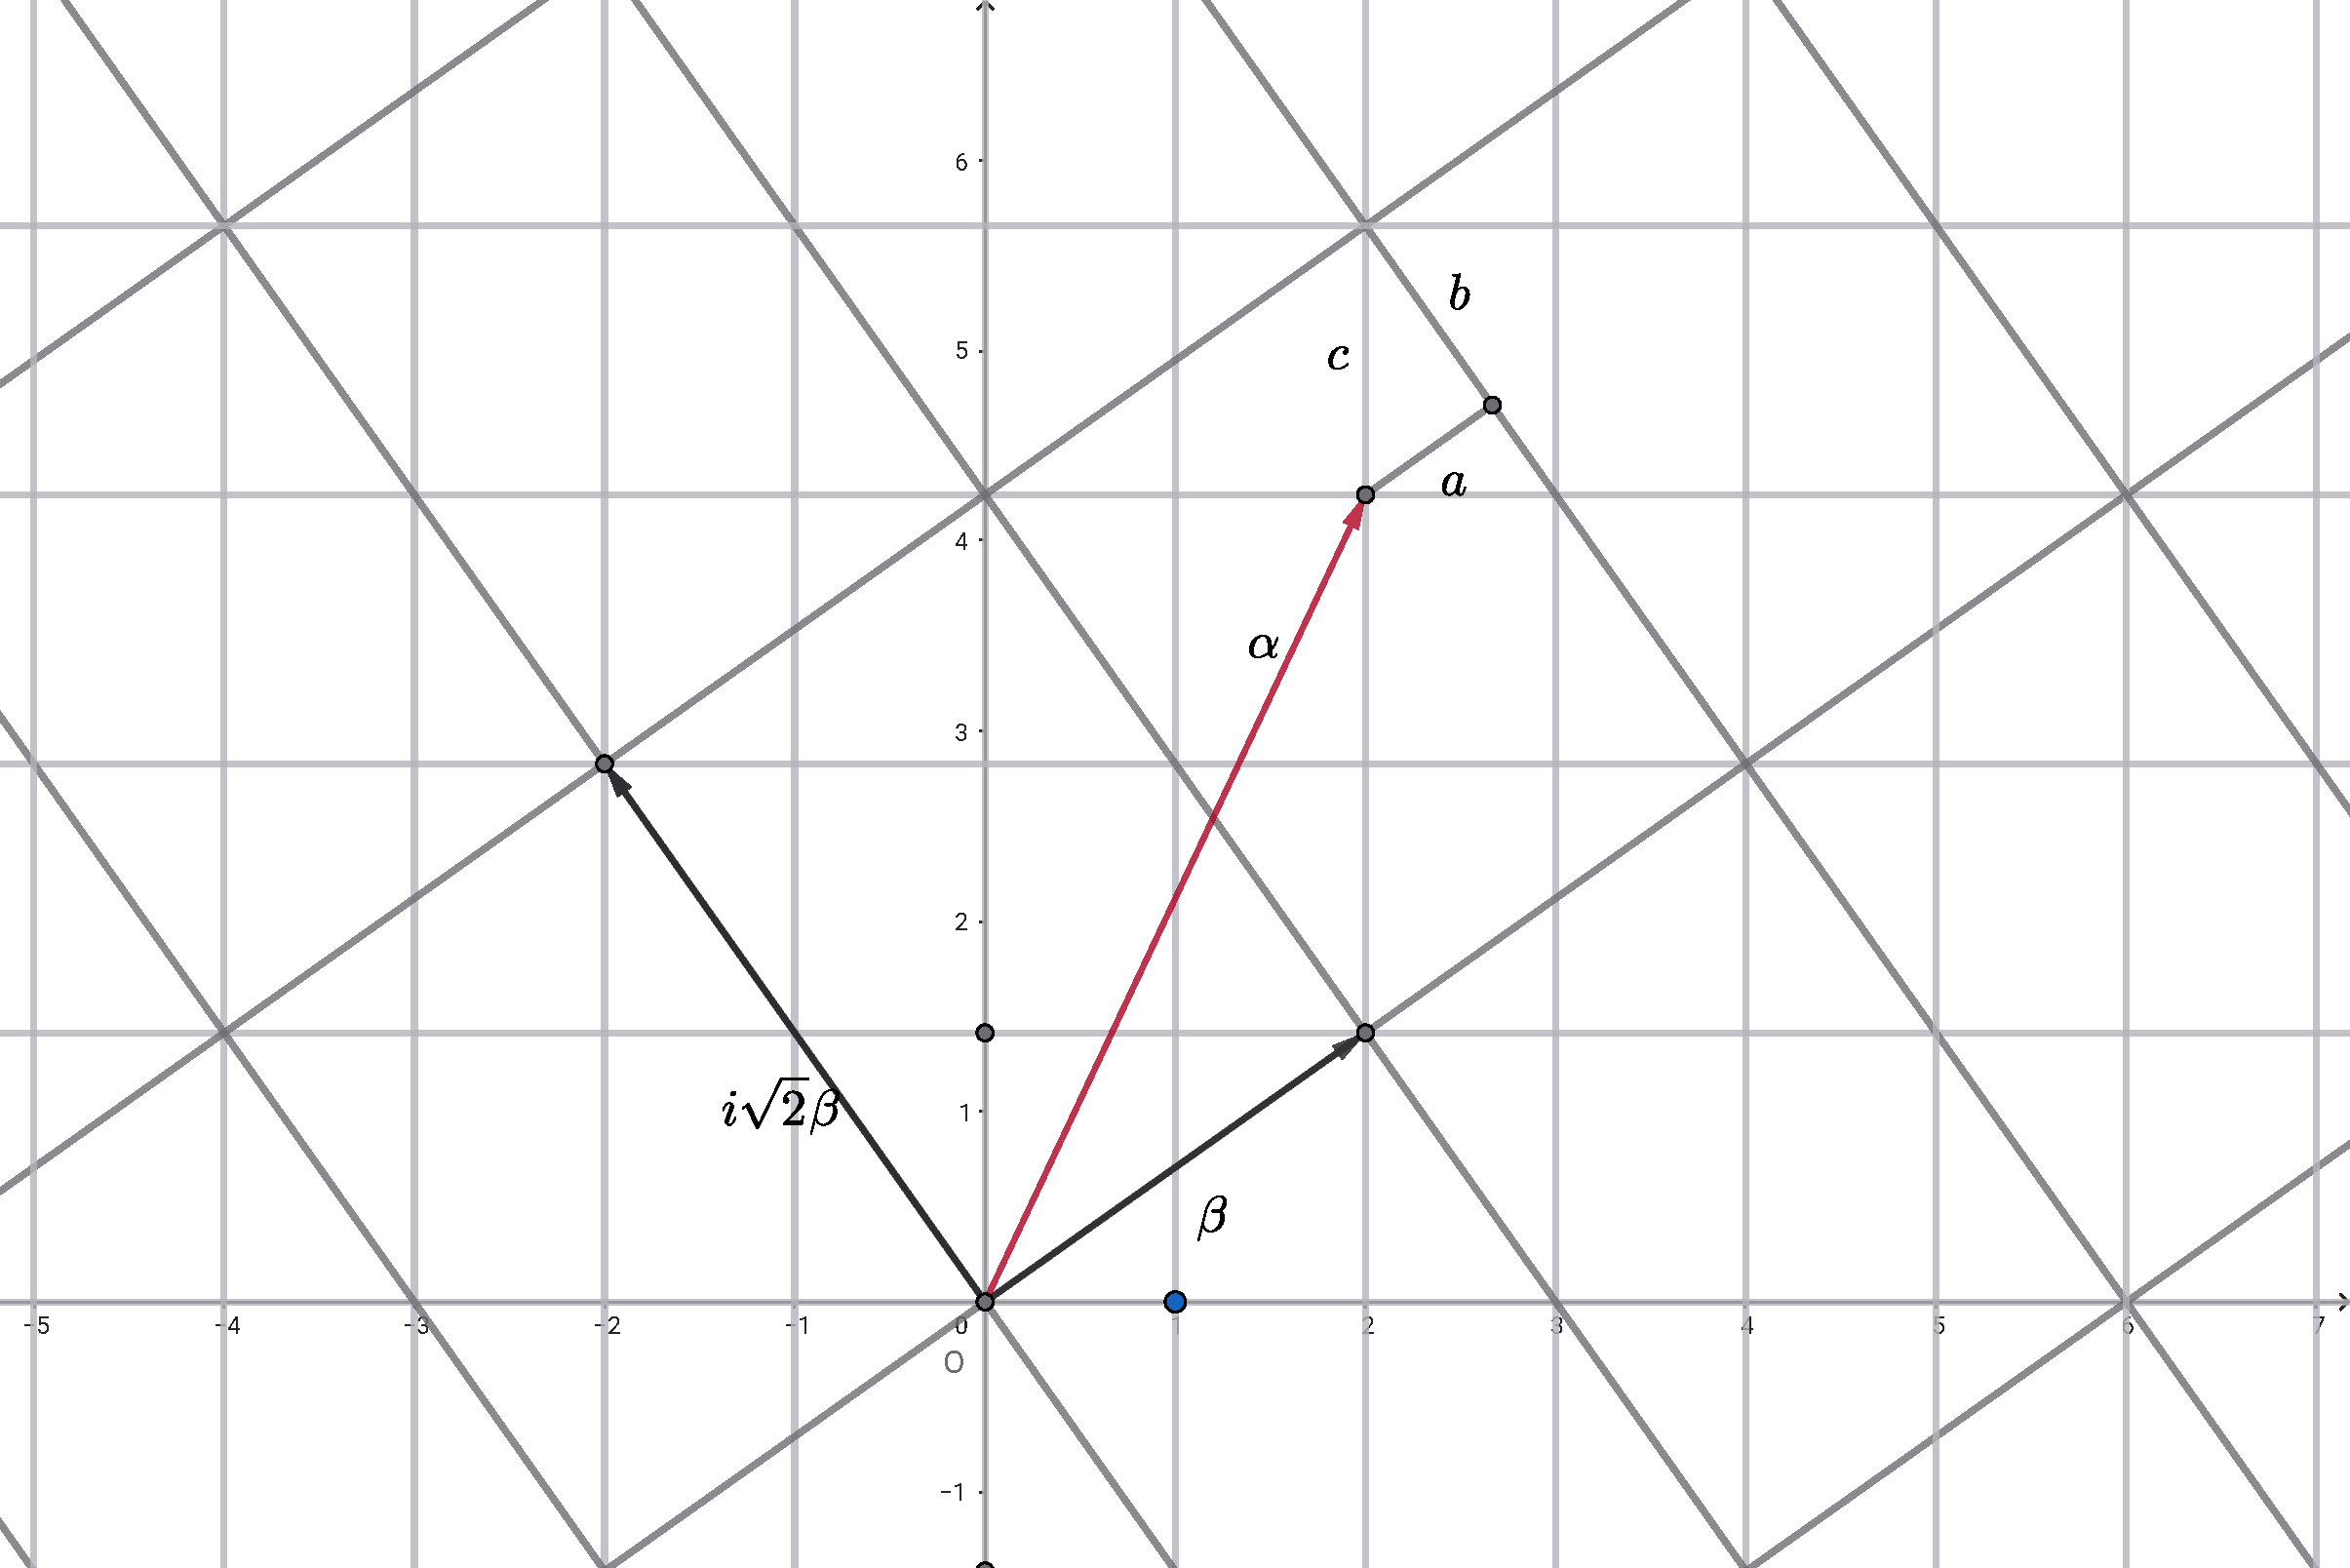
\includegraphics[scale=0.3]{img/z-sqrt-2}
 \caption{The quadratic integers in $\mathbb{Z}[\sqrt{-2}]$ form a lattice in gray color, those are the product of $\rho \beta$ form a lattice in black color. $\alpha$ lies in some rectangle.}
 \label{fig:Z-sqrt-2}
\end{figure}

\begin{align*}
N(\alpha - \rho\beta) & = c^2 = a^2 + b^2  && \text{by Pythagorean theorem} \\
  &\leq (\frac{\sqrt{2}}{2}|\beta|)^2 + (\frac{1}{2}|\beta|)^2 && a, b\text{ neither is longer than half side respectively} \\
  &= \frac{3}{4}|\beta|^2 < |\beta|^2 = N(\beta)
\end{align*}

Let $\gamma = \alpha - \rho \beta$ as needed. Therefore, Euclidean algorithm is valid in $\mathbb{Z}[\sqrt{-2}]$, it follows that the corresponding fundamental theorem of arithmetic is true. However, $\mathbb{Z}[\sqrt{-3}]$ breaks this pattern; here is a counter example:

\[
4 = 2 \times 2 = (1 + i\sqrt{3})(1 - i\sqrt{3})
\]

where 2 cannot be further factorized. Otherwise, suppose $2 = (a + b\sqrt{-3})(c + d\sqrt{-3})$, taking norm of both sides:

\[
4 = N(2) = N(a+b\sqrt{-3})N(c + d\sqrt{-3}) = (a^2 + 3b^2)(c^2 + 3d^2)
\]

It's impossible that $a^2 + 3b^2 = c^2 + 3d^2 = 2$, in other words, no solution to this equation in integers. Therefore, either $a^2 + 3b^2$ or $c^2 + 3d^2$ is 1, which corresponds to a unit; the other is an associate of 2. This shows 2 cannot be further factorized. The norms of $1 \pm i\sqrt{3}$ are both 4, one may show they cannot be further factorized in the same way. It turns out there are two distinct ways to factorize 4, in other words, not unique factorization. To understand why, as shown in \cref{fig:Z-sqrt-3}, the products of $\rho \beta$ form a lattice of rectangles spanned by $\beta$ and $i\sqrt{3}\beta$. Any $\alpha$ lies in some rectangle; the square of its distance to the closest corner is,

\begin{align*}
N(\alpha - \rho \beta) &= c^2 = a^2 + b^2  && \text{by Pythagorean theorem} \\
  &\leq (\frac{\sqrt{3}}{2}|\beta|)^2 + (\frac{1}{2}|\beta|)^2 = |\beta|^2 && a, b \leq \text{ half side}
\end{align*}

\begin{figure}[htbp]
 \centering
 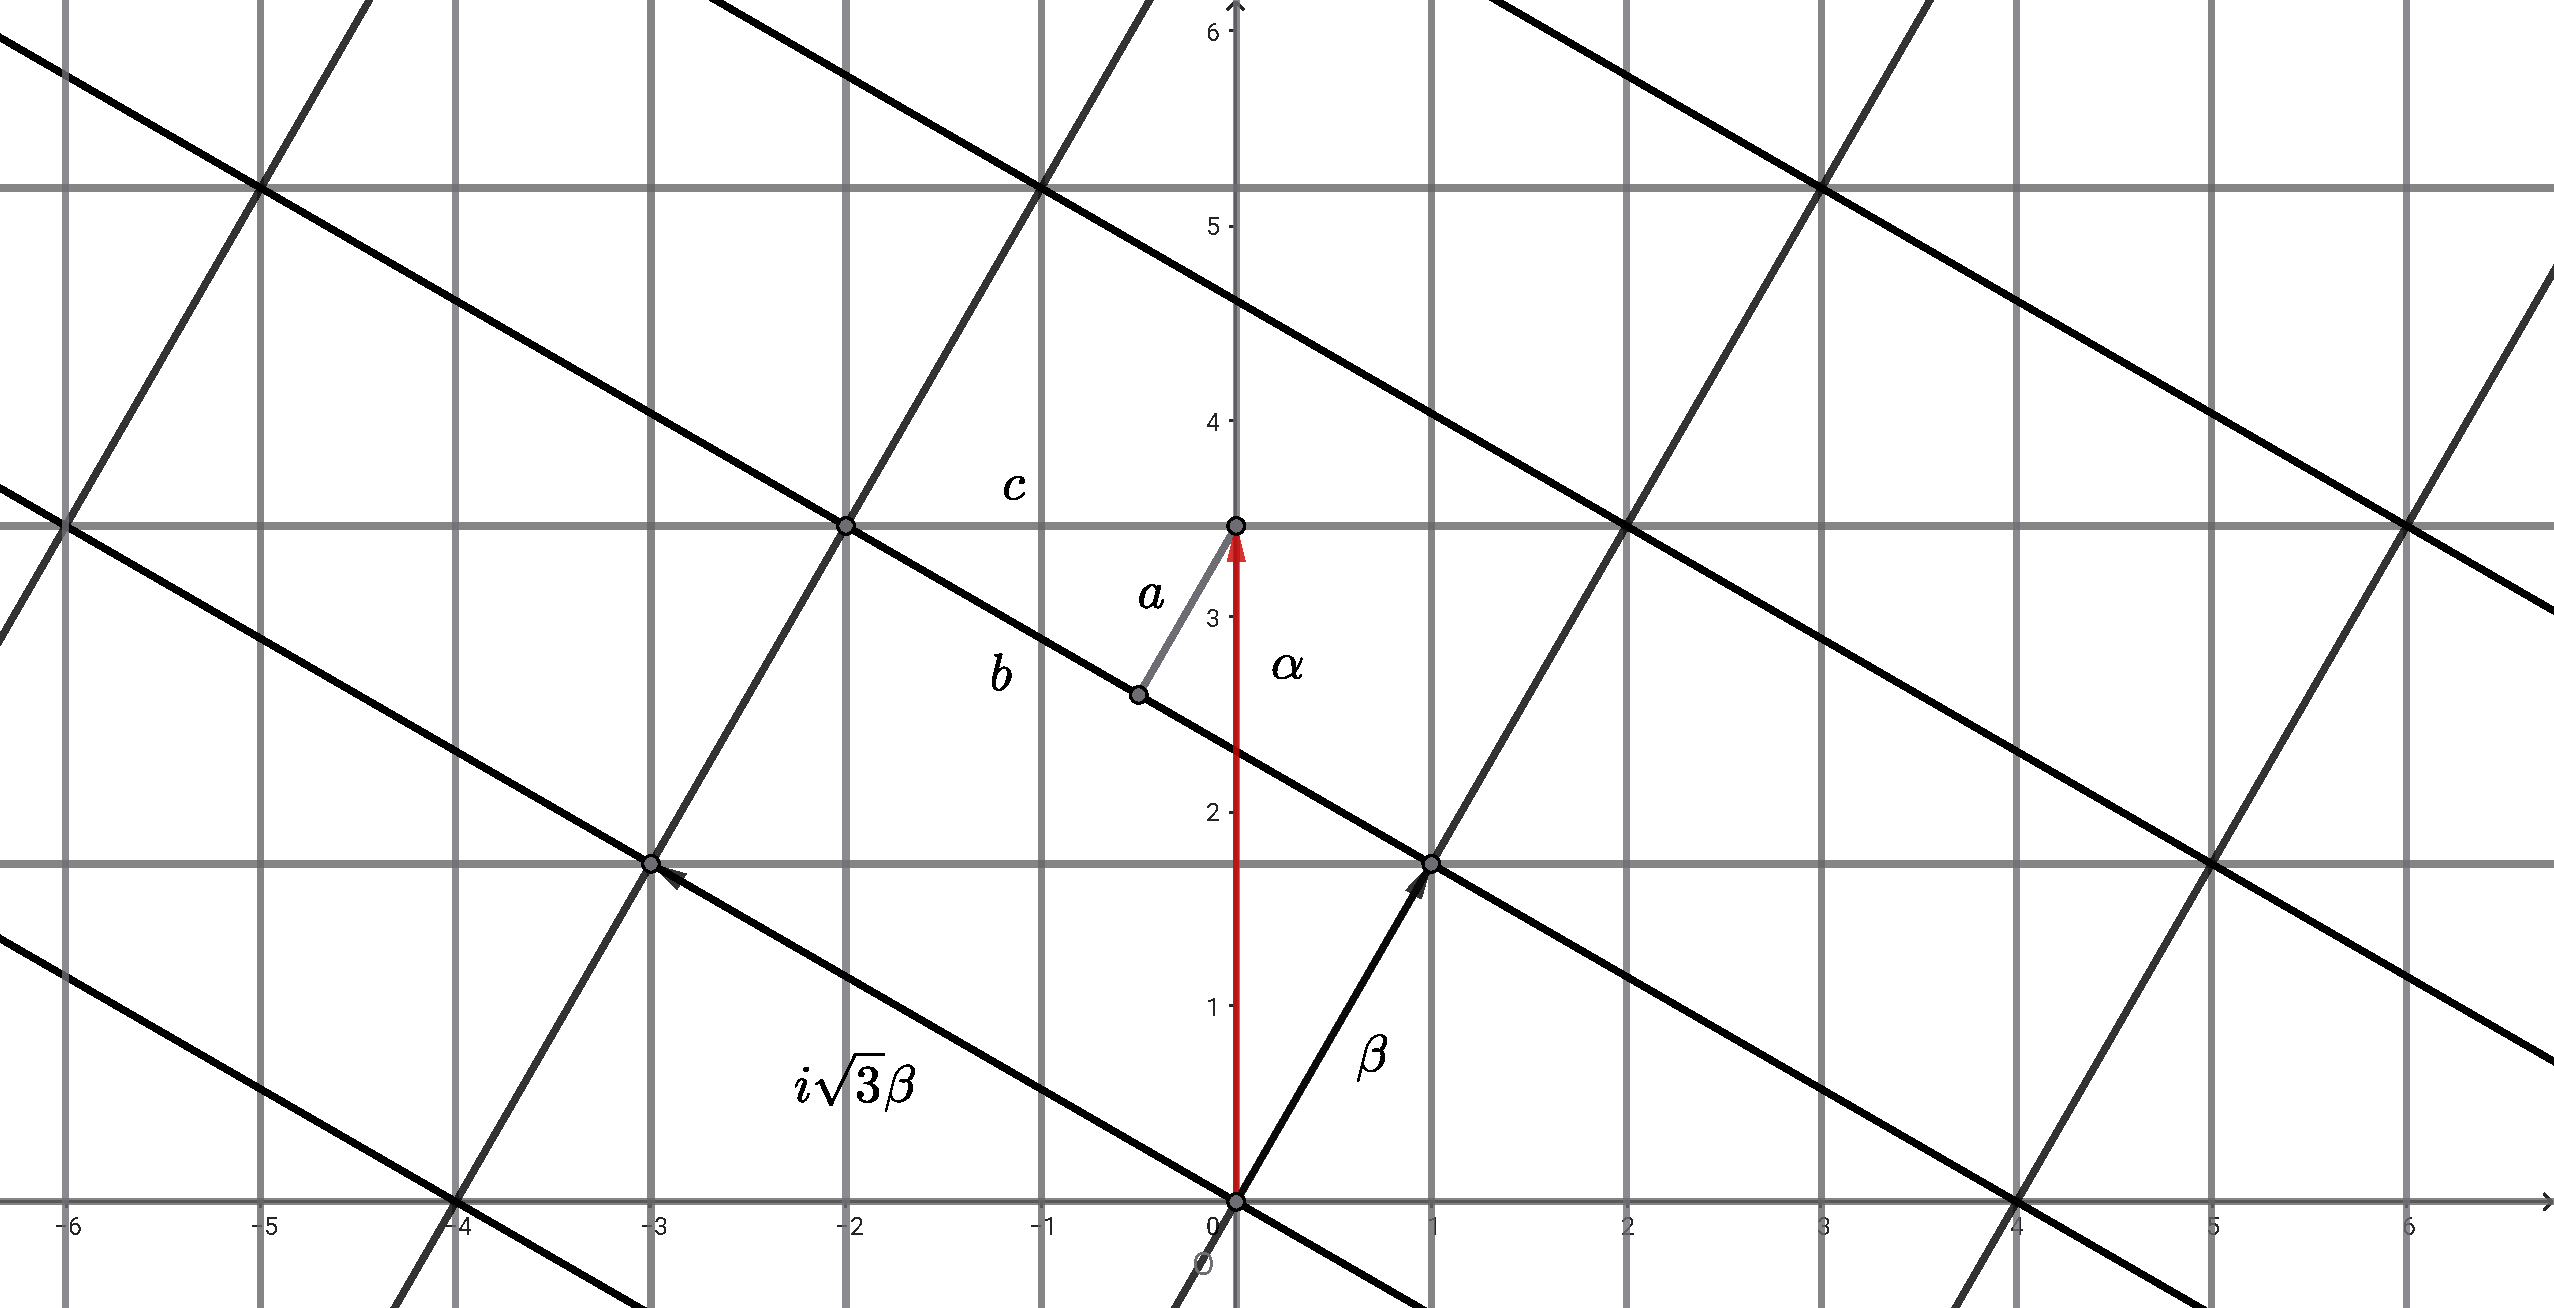
\includegraphics[scale=0.3]{img/z-sqrt-3}
 \caption{The quadratic integers in $\mathbb{Z}[\sqrt{-3}]$ form a lattice in gray color; the products of $\rho \beta$ form a lattice in black color; $\alpha$ lies in some rectangle.}
 \label{fig:Z-sqrt-3}
\end{figure}

It is not necessarily $<$. As shown in the figure, when $\alpha$ lies at the center of the rectangle, there does not exist $\gamma$ such that $N(\gamma) < N(\beta)$. Hence Euclidean algorithm isn't applicable to $\mathbb{Z}[\sqrt{-3}]$, in other words, the fundamental theorem of arithmetic isn't true, no unique factorization. This is why $4 = 2 \times 2 = (1 + i\sqrt{3})(1 - i\sqrt{3})$. What a pity! wherever $\alpha$ lies except for the center of the rectangle, the distance from it to the closest corner $< |\beta|$. Given that only the center is the exception, is there a way to save the unique factorization? As shown in \cref{fig:Z-omega}, the center of the rectangle $\notin \mathbb{Z}[\sqrt{-3}]$, in this case, for any integer $\alpha$, there exists some $\gamma$ satisfying $N(\gamma) < N(\beta)$. What's the difference between these two cases? It seems $\beta$ leads to different result.

\begin{figure}[htbp]
 \centering
 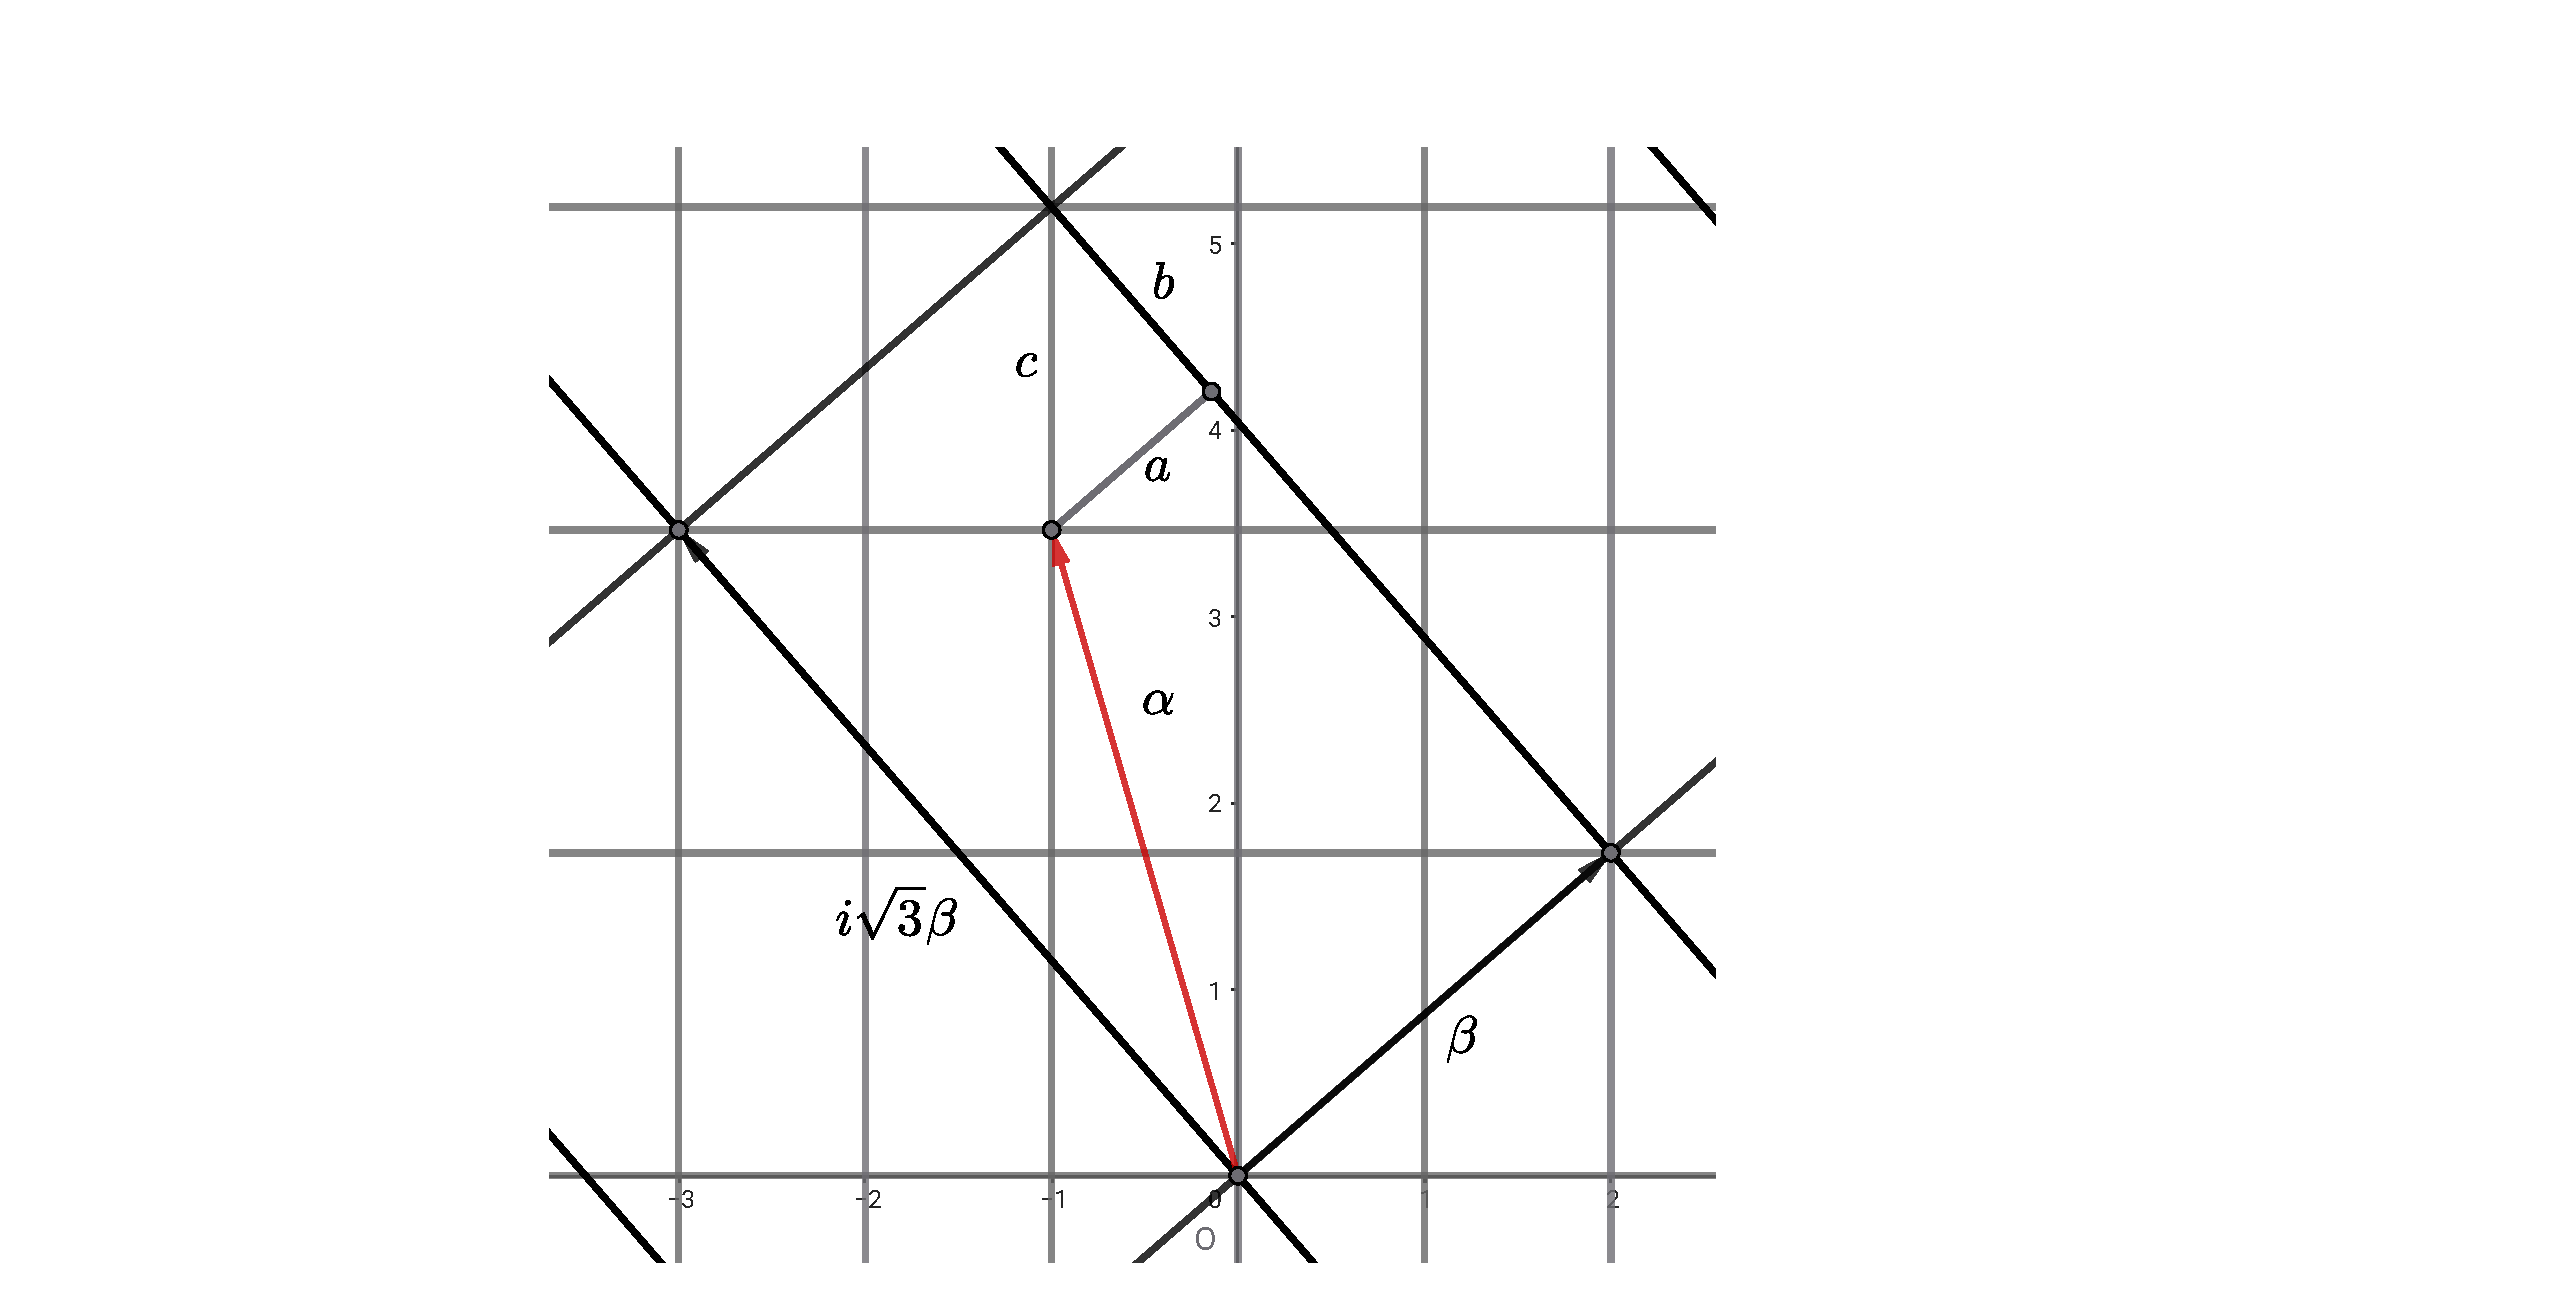
\includegraphics[scale=0.3]{img/z-omega}
 \caption{When $\beta = 2 + \sqrt{3}i$, any integer $\alpha$ does not lie at the center of the rectangles of $\rho \beta$. There exists some $\gamma$ satisfying $N(\gamma) < N(\beta)$.}
 \label{fig:Z-omega}
\end{figure}

Let's figure out in what condition, the center of the rectangle does not correspond to quadratic integer. As shown in \cref{fig:Z-sqrt-3c}, consider a rectangle spanned by some $\rho \beta$. The bottom left corner $A$ corresponds to vector $\rho \beta$. By the geometric interpretation of the sum of complex numbers, the bottom right corner $C$ corresponds to vector $\rho \beta + \beta$; the upper left corner $C'$ corresponds to $\rho \beta + i\sqrt{3}\beta$, which rotates the vector $\beta$ by 90 degrees, then scales up by $\sqrt{3}$ times, then adds to $C$. The center of the rectangle is the middle point of diagonal $CC'$, which corresponds to vector:

\[
\frac{C + C'}{2} = \frac{\rho \beta + \beta + \rho \beta + i\sqrt{3}\beta}{2} = \rho \beta + \frac{1}{2}\beta + \frac{\sqrt{3}}{2}i\beta
\]

\begin{figure}[htbp]
 \centering
 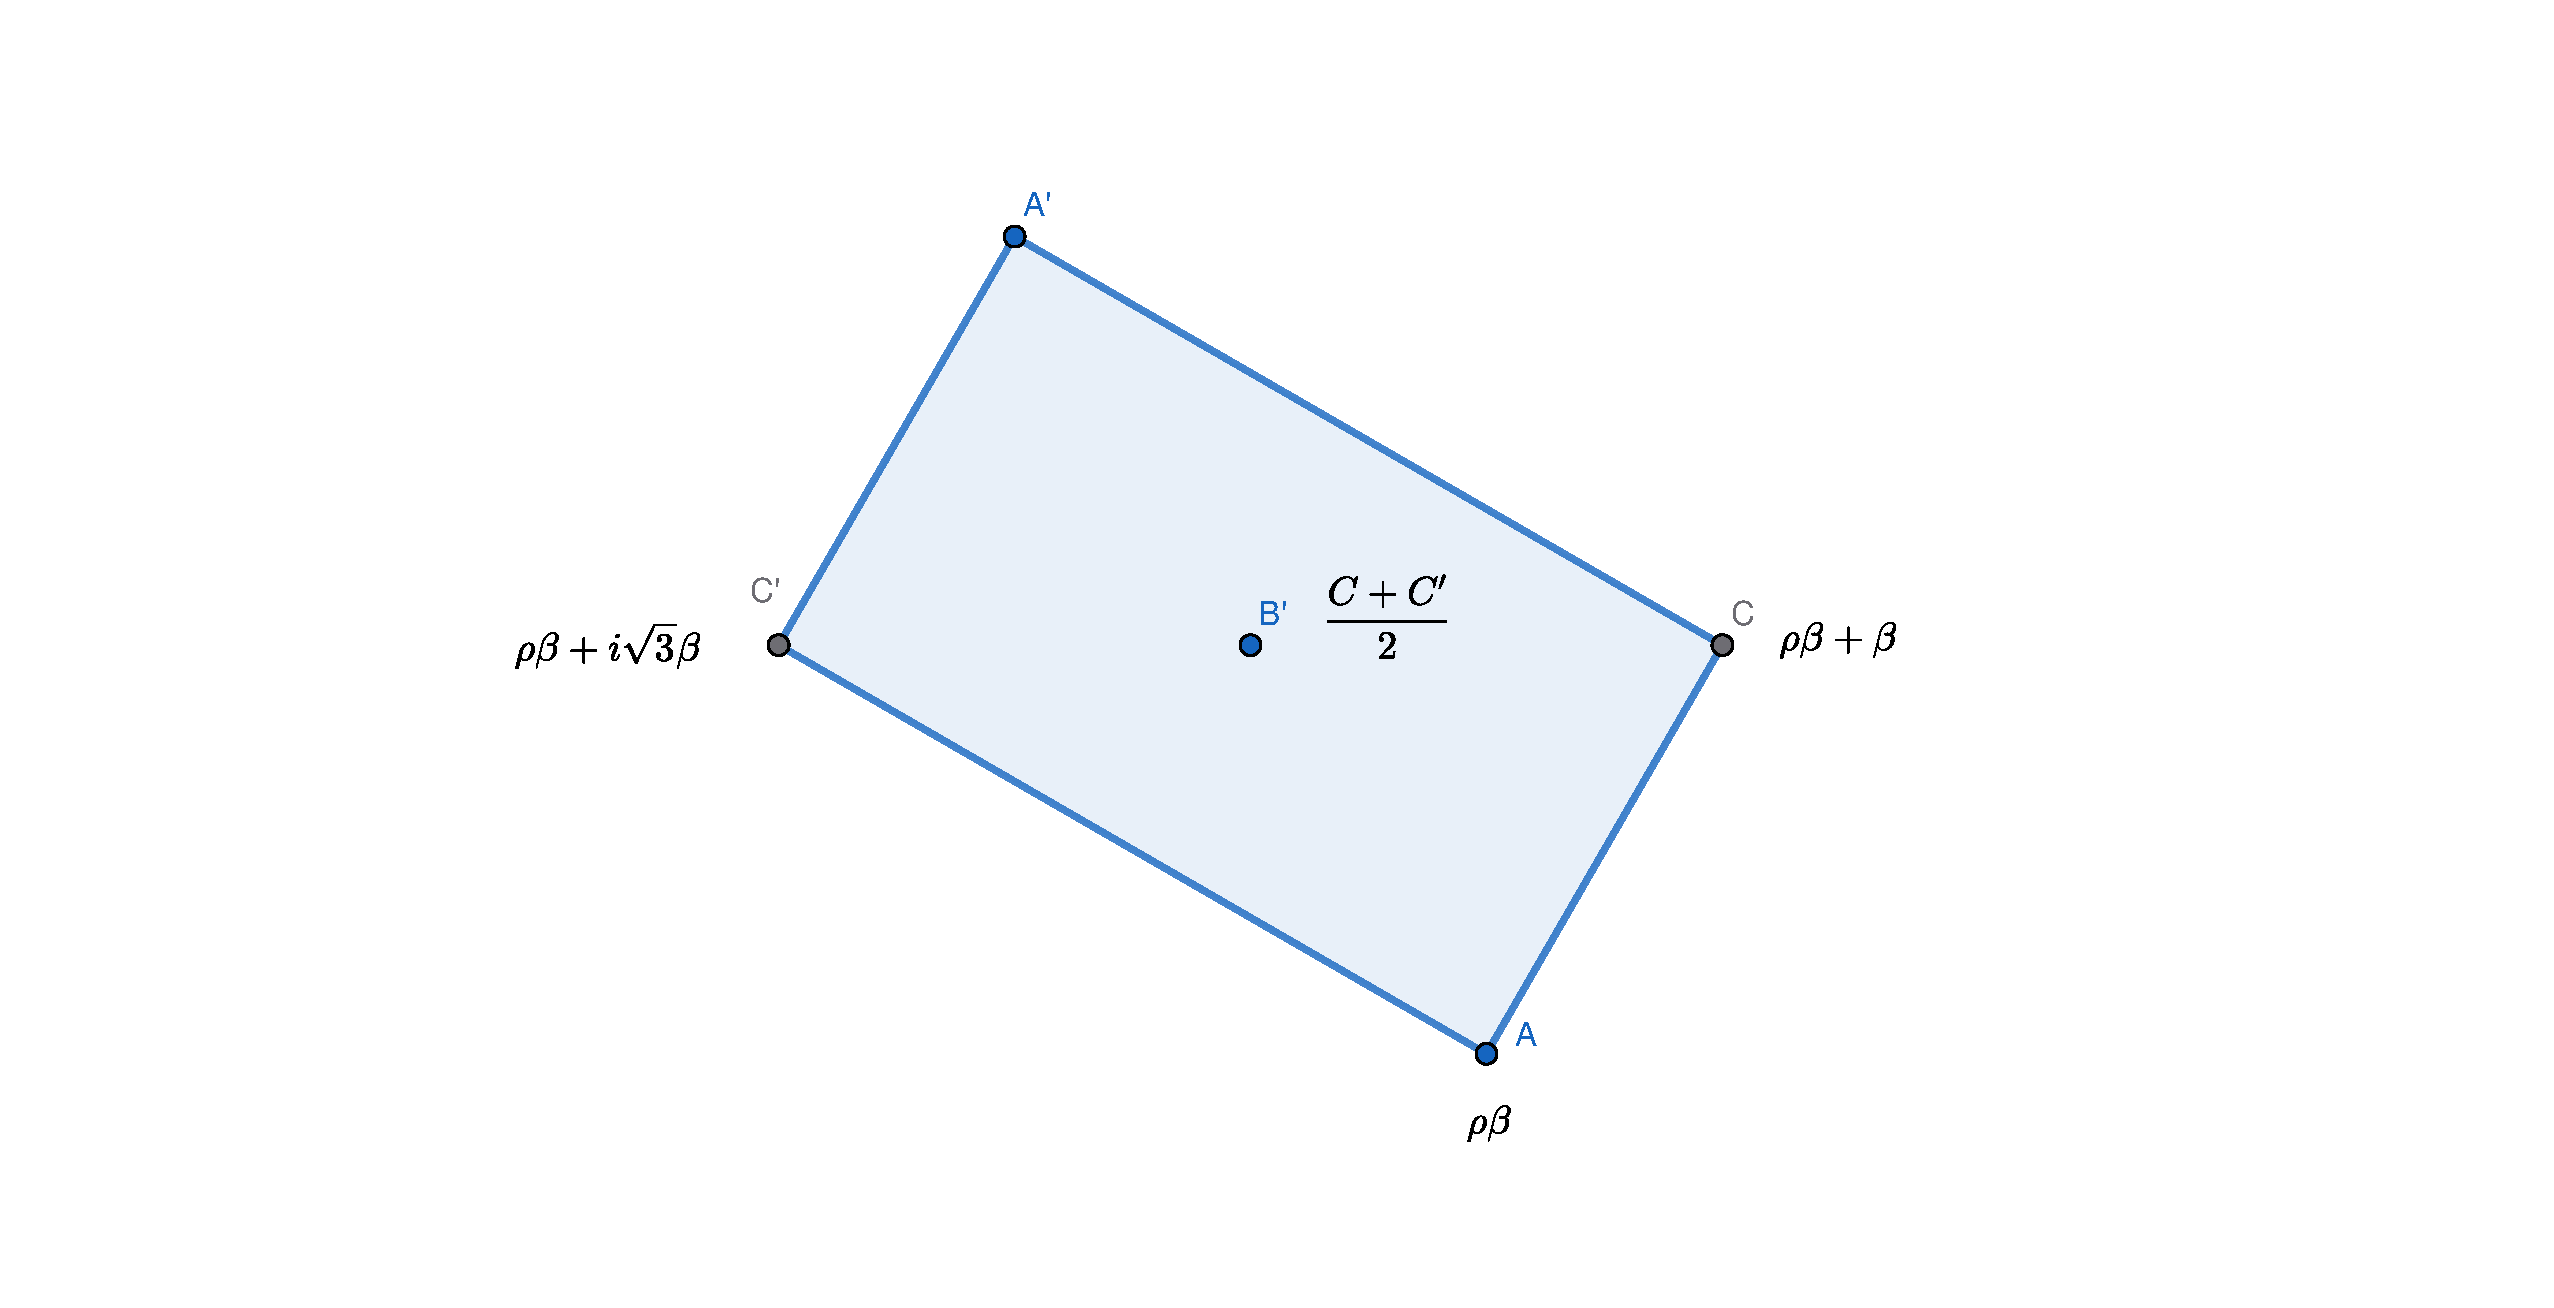
\includegraphics[scale=0.3]{img/z-sqrt-3c}
 \caption{A rectangle of $\rho \beta$ and its center.}
 \label{fig:Z-sqrt-3c}
\end{figure}

Since $\rho \beta \in \mathbb{Z}[\sqrt{-3}]$, when $\dfrac{1}{2}\beta + \dfrac{\sqrt{3}}{2}i\beta \notin \mathbb{Z}[\sqrt{-3}]$, the center of the rectangle does not correspond to any quadratic integer. Let $\beta = a + bi\sqrt{3}$ and substitute into:

\[
\frac{a + bi\sqrt{3}}{2} + \frac{(a + bi\sqrt{3})i\sqrt{3}}{2} = \frac{a - 3b}{2} + \frac{a + b}{2}i\sqrt{3}
\]

If $a-3b$ or $a + b$ is odd, then the center of the rectangle does not correspond to quadratic integer; in this case, the parity of $a, b$ is different. Conversely, if the parity of $a, b$ are same, the center of the rectangle corresponds to some quadratic integer, the Euclidean algorithm is invalid. For the counter example of $4 = 2 \times 2 = (1 + i\sqrt{3})(1 - i\sqrt{3})$, indeed $a = b = 1$ both are odd. While in the case of \cref{fig:Z-omega}, $\beta = 2 + i\sqrt{3}$, where $a = 2, b=1$ are in different parity, hence $\alpha$ cannot lie at the center of the rectangle, Euclidean algorithm is valid, and unique factorization hold. In Euler's proof to Fermat's Last Theorem of $n=3$, indeed it demands $a, b$ in different parity, which asserts unique factorization. Therefore, when $a^2 + 3b^2$ is a cube, the relatively prime $(a + bi\sqrt{3})(a - bi\sqrt{3})$ each is a cube (\cref{qn:coprime-of-conjugates} asks to show $a \pm bi\sqrt{3}$ are relatively prime).

\index{Eisenstein integers}
This completes the proof of Fermat's Last Theorem of $n=3$. The story of $\mathbb{Z}[\sqrt{-3}]$ continues. Gaussian integers lie in the lattice of squares in complex plain. Eisenstein (\cref{fig:Eisenstein}) in 1844 studied the complex integers lie in the lattice of equilateral triangles, which are called Eisenstein integers nowadays. The two roots of monic quadratic equation $x^2 + x + 1 = 0$ are $\omega = \dfrac{-1}{2} \pm \dfrac{i\sqrt{3}}{2}$. By the definition of algebraic integers, though with terms of $\dfrac{1}{2}$, they are all algebraic integers! More generally, the roots of monic quadratic equation $x^2 - (2a - b)x + (a^2 - ab + b^2)$ are in the form of $a + b \omega$. They form Eisenstein integers, denoted by $\mathbb{Z}[\omega]$. Eisenstein defined the norm as $N(a + b\omega) = a^2 -ab + b^2$ (see \cref{qn:norm-of-z-omega}), and showed that Euclidean algorithm existed in $\mathbb{Z}[\omega]$, hence unique factorization held. Actually, $\mathbb{Z}[\sqrt{-3}]$ is just a subset of $\mathbb{Z}[\omega]$.

\begin{figure}[htbp]
  \centering
  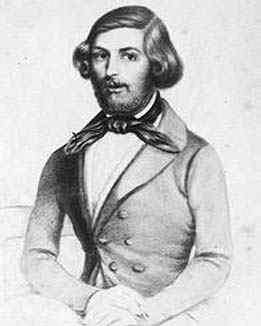
\includegraphics[scale=0.4]{img/Eisenstein}
  \caption{Eisenstein, 1823 - 1852}
 \label{fig:Eisenstein}
\end{figure}

\index{Eisenstein}
\begin{mdframed}
André Weil wrote a fantastic biography for Gotthold Eisenstein (1823 - 1852) in his book reviews for \emph{Mathematische Werke, by Gotthold Eisenstein}\cite{Weil-2024}.

\begin{quotation}
On the 16th of April, 1823, a number of fairies, summoned by Ganesha, the god of mathematical wisdom, assembled in Berlin at the cradle of an infant, to grant boons and bestow blessings. This was the first-born of a not too prosperous businessman who had married in June of the previous year; both parents were Jewish but had been baptized into the evangelical faith. Alas, as in all fairy tales, one old witch managed to creep in and resolved to undo, if she could, the work of the fairies.

\enquote{He will have genius,} said the first fairy, \enquote{and will be a worthy successor of Gauss, Dirichlet, Jacobi.} -\enquote{His life will be short and unhappy,} said the witch. -\enquote{He will have many brothers and sisters,} said the next fairy, \enquote{and will be tenderly attached to them, while remaining his mother's favorite.} -\enquote{He will lose them all,} said the witch; \enquote{seventeen years from now he will see the last one, a beloved small sister, die at the age of seven.} -\enquote{He will have brilliant teachers at the Gymnasium and will make giant strides in his mathematical studies.} -\enquote{But first,} said the witch, \enquote{his parents will misguidedly send him for four years to a private school whose rigid discipline will almost break his already fragile health and make him a nervous wreck for the rest of his life.} -\enquote{In his first year as a student at the University of Berlin, he will attract the attention of Humboldt, the grand old man of German science, and of Crelle, the editor of the leading mathematical journal of his time, and will have more than twenty papers accepted by Crelle that same year.} -\enquote{Maybe,} said the witch; \enquote{but first, for his support at the University, his mother will have to accept a paltry sum from the royal \enquote{indigent fund}.} -\enquote{So what?} said one big fairy with a strong American accent. \enquote{Soon Humboldt will get him a yearly grant of 250 dollars 1 from the RSF, and will get it renewed when needed.} -\enquote{O.K.,} retorted the witch; \enquote{but uncertainties about the payment and renewal of this stipend will plague and humiliate him for the rest of his life.} -\enquote{No matter,} said the next fairy. \enquote{Gauss, one of the hardest men to please in the mathematical world, will invite him, still a first-year student, to a visit in Göttingen, and from then on will take the deepest interest, not only in his work but also in his well-being. Jacobi, intent upon making him a \enquote{privatdozent} and anxious to cut bureaucratic red tape, will arrange for him to receive an honorary doctorate at the hands of Kummer in Breslau: surely an unheard-of favor to a second-year student! Gauss, while proposing Dirichlet for a coveted distinction (the order \enquote{Pour le mérite}), will let it be known that he has \enquote{almost hesitated} between him and young Eisenstein.} -\enquote{Much good this will do him!} exclaimed the witch with a sneer. \enquote{It will so enrage Jacobi that he will practically accuse your darling of plagiarism, in a wholly unmotivated footnote in Crelle's Journal.} -\enquote{Who knows not what the easily inflamed Jacobi can do once his temper is aroused?} said another good fairy. \enquote{This incident will deeply distress the young man for a while but will do him no further harm. Soon he will be a privatdozent, and the great Riemann will be one of his students.} -\enquote{Not for long! Riemann will migrate to Göttingen and forget whatever number-theory his young teacher thinks he has taught him. In the meanwhile, I will have seen to it that Kronecker and Heine leave Berlin; the young man will remain isolated without any congenial friend or companion.} One fairy thought that Gauss' name had such virtue that it would silence the malevolent creature: \enquote{In 1847, the great Gauss will write a highly flattering foreword for a collection of his protege's papers.} -\enquote{Hardly anyone will read them,} replied the witch with utter contempt. \enquote{Then he will be so beaten up by the Prussian soldiery, during the revolutionary upheavals of 1848, that he will have to keep to his bed for a week; for two years he will publish nothing, and the reputation of being \enquote{red} will stick to him and threaten to jeopardize his stipend and his career.} -\enquote{He will not remain idle during those two years, in spite of all discouragement and ill health; his publications of the year 1850 will show him at the peak of his powers. Dirichlet, with Jacobi's concurrence, will propose him for membership in the Berlin Academy, and he will finally be elected in 1852, as Jacobi's successor, a young man of not yet 29 years of age.} -\enquote{And then he will die, said the witch triumphantly.} -\enquote{But his name will survive, said a tiny fairy.} -\enquote{Hardly so,} said the hag. \enquote{Following academic usage, Dirichlet will read to the Academy a beautiful and moving eulogy of Jacobi, and Kummer will perform the same service for Dirichlet. But no member of the Academy will ever bother about the memory of the melancholy young man who had died in 1852. Still less will it occur to them to provide for the publication of his works, while voting ample funds for those of Jacobi, Dirichlet, Steiner, and later for Weierstrass and Kronecker. He will be forgotten, once and for all.} -\enquote{It is lucky,} said one last fairy in a small voice, \enquote{that you remind me of Kronecker. For many years, your curse will indeed prevent him from remembering the companion of his youth. But I will cause him to rediscover his friend's work before it is too late, and he will make it the theme of the main lecture to be given at the inauguration ceremonies of the German Mathematical Society.} The witch laughed loudly. \enquote{It will be too late! I will kill Kronecker's wife, and he will cancel his lecture.} -\enquote{He will offer to write it up.} -\enquote{Before he does, I will kill him too, and then that name, which I do not want even to utter, will sink into final oblivion.} There were no more fairies; but Ganesha had the last word. \enquote{You forget,} he said, \enquote{that all your curses are of limited duration; one hundred and fifty years from today, their force will be spent.}
\end{quotation}
\end{mdframed}

It is just lucky that the fundamental theorem of arithmetic is applicable to $\mathbb{Z}[\sqrt{-2}]$ and $\mathbb{Z}[\omega]$ as it isn't valid in common. For example, $6 = 2 \times 3 = (1 + i\sqrt{5})(1 - i\sqrt{5})$ in $\mathbb{Z}[\sqrt{-5}]$. One may show that none of $2, 3, 1 \pm i\sqrt{5}$ can be further factorized. Otherwise, suppose 2 can be factorized into $(a + bi\sqrt{5})(c + di\sqrt{5})$, taking norm of both sides:

\[
4 = N(2) = N(a + bi\sqrt{5})N(c + di\sqrt{5}) = (a^2 + 5b^2)(c^2 + 5d^2）
\]

We may first rule out the case of $a^2 + 5b^2 = c^2 + 5d^2 = 2$ as none integers of $a, b, c, d$ satisfying it. The only possibility is $a^2 + 5b^2 = 1$ or $c^2 + 5d^2 = 1$. The norm of 1 corresponds to unit and the other corresponds to associate of 2, which shows 2 cannot be further factorized. In the same way, 3 cannot be further factorized. \Cref{qn:1-n-delta-irreducible} asks to show $1 \pm i\sqrt{5}$ cannot be further factorized in this way. It turns out that $6 = 2 \times 3 = (1 + i\sqrt{5})(1 - i\sqrt{5})$, having two distinct ways of factorization. To save the unique factorization, Kummer introduced ideal numbers, which was further developed by Dedekind to a powerful tool -- ideal.

\section{Ideals}
\index{ideals}
Here is a homework problem about set theory taken from the mathematical exercise book for grade K10 students in China\footnote{Set theory is the first unit in K10 school math in China.}.

\begin{mdframed}
Given two non-empty set $I, P$, define $I$ is a \enquote{ideal subset} of $P$ if it satisfies the following:

\begin{enumerate}[(i)]
\item $x \in P$ for every $x \in I$;
\item $x + y \in I$ for any $x, y \in I$;
\item $xy \in I$ for any $x \in I$ and any $y \in P$.
\end{enumerate}

Select \emph{all} correct ones from below statements:

\begin{enumerate}[(a)]
%%   \renewcommand{\labelenumi}{\textcircled{\theenumi}}
\item If $I = \{2k | k \in \mathbb{Z} \}$, then $I$ is a \enquote{ideal subset} of $\mathbb{Z}$;
\item If $I$ is a \enquote{ideal subset} of $\mathbb{R}$, and there exists some non-zero real number $a \in I$, then $I = \mathbb{R}$;
\item If $I_1, I_2$ are \enquote{ideal subsets} of $P$, then $I_1 \cup I_2$ is a \enquote{ideal subset} of $P$ too;
\item if $I_1, I_2$ are \enquote{ideal subsets} of $P$, then $I_1 \cap I_2$ is a \enquote{ideal subset} of $P$ too.
\end{enumerate}

The correct ones are: $\underline{\qquad \qquad}$

\end{mdframed}

It only needs elementary set theory to solve this exercise. Property (i) shows $I$ is a subset of $P$; property (ii) states that $I$ is closed under addition, that is, the sum of any two numbers in $I$ is still in $I$; property (iii), though not so direct, states that if scale any $x$ in $I$ by a factor $y$ in $P$, the result $xy$ is in $I$. we may say $I$ is closed under the scaling by $P$. Now let see the four options. For option (a), $I$ is the set of even numbers. Since every even number is an integer, property (i) holds; the sum of two even numbers is still even, hence property (ii) holds; the product of an even number and an integer is always even, hence property (iii) holds. Therefore, the set of even number is an \enquote{ideal subset} of integers; option (a) is true. For option (b), the key point is whether 1 is in $I$. As $a \ne 0$, its reciprocal $\dfrac{1}{a} \in \mathbb{R}$ exists. Now $a \in I, \dfrac{1}{a} \in \mathbb{R}$, by property (iii), $a\dfrac{1}{a} = 1 \in I$. Once 1 is in $I$, then for any real number $x \in \mathbb{R}$, by property (iii), we have $1 \cdot x = x \in I$, hence $\mathbb{R}$ is a subset of $I$. Meanwhile, property (i) implies $I$ is a subset of $\mathbb{R}$, it turns out that $I = \mathbb{R}$. Therefore, option (b) is true. We may examine option (c) with some concrete example. Analogue to even numbers in option (a), let $I_1 = \{2k | k \in \mathbb{Z} \}, I_2 = \{5k | k \in \mathbb{Z} \}$, we can verify that $I_2$, the multiples of 5, is also an \enquote{ideal subset}. Their union contains even numbers and multiples of 5: $\{ \dotsc, 0, 2, 4, 5, 6, \dotsc\}$; but $2 + 5 = 7$ is not in this set, not closed under addition, breaks property (ii). Therefore, option (c) is false. Option (d) replaces union by intersection. Examine the same example: $I_1$ of even numbers and $I_2$ of multiples of 5; their intersection contains all even multiples of 5: $\{\dotsc, -10, 0, 10, 20, \dotsc\}$. It's easy to verify this is an ideal subset. Let's further prove it.

\begin{proof}
For any $x \in I_1 \cap I_2$, we have $x \in I_1 \subseteq P$, hence property (i) holds. For any $x, y \in I_1 \cap I_2$, we have $x, y \in I_1$; since $I_1$ is an \enquote{ideal subset}, hence $x + y \in I_1$. Meanwhile, $x, y \in I_2$ and $I_2$ is also an \enquote{ideal subset}, hence $x + y \in I_2$. It follows that $x + y$ is in both $I_1$ and $I_2$, therefore, $x + y \in I_1 \cap I_2$. This shows $I_1 \cap I_2$ is closed under addition, satisfying property (ii). Finally, for any $x \in I_1 \cap I_2, y \in P$, as $x \in I_1$ and $I_1$ is an \enquote{ideal subset}, hence $xy \in I_1$. Meanwhile, as $x \in I_2$ and $I_2$ is also an \enquote{ideal subset}, hence $xy \in I_2$. Thus $xy$ is in both $I_1$ and $I_2$, therefore, $xy \in I_1 \cap I_2$, satisfying property (iii). This proves $I_1 \cap I_2$ is an \enquote{ideal subset}.
\end{proof}

Thus the correct options are: $\underline{(a), (b), (d)}$。

\index{ring} \index{principal ideal}
This interesting exercise is exactly how Dedekind defines the concept of ideal! The only additional thing is that Dedekind requires the parent set $P$ to be a \enquote{ring}. Basically, a ring is a set with addition, multiplication, 0 and 1, containing positive and negative elements\footnote{Accurately speaking, a \emph{commutative} ring satisfies associative and commutative law for addition and multiplication, and contains 0, 1, positive and negative elements. For example, the sets of integers, Gaussian integers, quadratic integers are all rings. Because containing negative numbers, they are closed under addition and subtraction.}. We'll use symbol $R$ to represent a ring in the future. For the non-unique factorization $6 = 2 \times 3 = (1 + i\sqrt{5})(1 - i\sqrt{5})$, Kummer introduced \enquote{ideal numbers}, which could further factorize $2, 3, 1 \pm i\sqrt{5}$, such that the final factorization in ideal numbers was unique. But what are exactly ideal numbers? Dedekind gave an astonishing answer: an ideal is not a concrete number any longer, but a set of number, and the set is infinite! For example, all even numbers, which are infinitely many multiples of 2; denote this ideal by $(2)$, similarly, denote all multiples of 5 by $(5)$. An ideal $I$ is called \emph{principal ideal} if it a set of all multiples of some $a$, denoted by $(a)$. The definition of ideal is quite different from other numbers we've seen so far. Gottlob Frege was the first logician who defined numbers in set. Numbers are abstract, for example, 3 as a number can represents three men, three eggs, three angles (in some shape) and so on; all these classes\footnote{Prior to Cantor, Frege used the term \enquote{class}, while Cantor later used \enquote{set}.} contains three things. But in turn which one should be used to represent natural number 3? Frege's idea was \emph{all}, all such classes that 1-to-1 corresponded. This is an infinite, abstract class that defines natural number 3. Although a bit complex, it's a great definition that free from culture limitation. No matter what language or what symbol is using, there won't be any ambiguities to understand number 3 through Frege's way.

\index{Frege}
\begin{figure}[htbp]
 \centering
 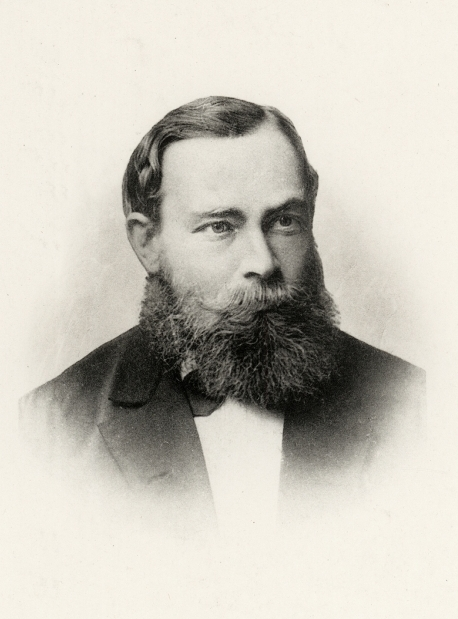
\includegraphics[scale=0.9]{img/Frege}
 \caption{Gottlob Frege, 1848 - 1925}
 \label{fig:Frege}
\end{figure}

But how can ideals save unique factorization? Dedekind firstly redefined division, the greatest common divisor, and etc., in the language of ideals. For natural numbers, we say 2 divides 6 and 3 divides 5, the greatest common divisor of 2 and 3 is $(2, 3) = 1$. Consider the ideals of $(2), (3)$, and $(6)$: (2) is the set of all even numbers, (6) is the set of all multiples of 6; but every multiple of 6 is also an even number, hence (2) contains (6); (3) is the set of all multiples of 3, and every multiple of 6 is also a multiple of 3, hence (3) contains (6).

\btab{c||c}
2 divides 6 & 3 divides 6 \\
(2) contains (6) & (3) contains (6)
\etab

We see the relation of dividing corresponds to containing, which may be summed up by the slogan \emph{to divide is to contain.} Actually, we may prove this correspondence.

\begin{proposition}
$a$ divides $b$，if and only if ideal $(a)$ contains ideal $(b)$.
\end{proposition}

\begin{proof}
By definition, there is some $c$ such that $ac = b$. Any $x \in (b)$ can be expressed as,
\begin{align*}
x &= bk  &&\text{where }k \in R \\
  &= ack &&\text{by definition of dividing} \\
  &= ak' \in (a) &&\text{let }k' = ck \in R \qedhere
\end{align*}

Conversely, since $(a)$ contains $(b)$, $b$ is in $(a)$, which consists of all multiples of $a$. Therefore, $b$ is also a multiple of $a$, hence $a$ divides $b$.
\end{proof}

\index{ideal!sum}
Next consider the greatest common divisor. Define the addition of ideals as $I_1 + I_2 = \{a + b | a \in I_1, b \in I_2\}$ (\Cref{qn:sum-of-ideals} asks to show the sum of ideals is an ideal). Thus the sum in above example is,

\[
(2) + (3) = \{a + b| a \in (2), b \in (3)\} = \{2x + 3y | x, y \in \mathbb{Z} \}
\]

Which is the set of numbers generated by 2 and 3, denote this sum of ideals by $(2, 3)$. One may notice the notation of the greatest common divisor happens to be the same. Indeed, the greatest common divisor of 2 and 3 is $d = (2, 3) = 1$, and by definition, $d$ divides both 2 and 3, hence $d$ divides every $2x + 3y$; therefore, the sum of ideals is $(d)$, which is (1).

\[
(2) + (3) = \{2x + 3y\} = \{dk | k \in \mathbb{Z}\} = (d) = (1)
\]

We summarize this result as below:
\begin{proposition}
If the greatest common divisor of $a$ and $b$ is $d = (a, b)$, then the sum of ideals$(a) + (b) = (d)$.
\end{proposition}

\begin{proof}
By definition:
\begin{align*}
(a) + (b) &= \{ax + by | x, y \in R\} \\
  &= \{dmx + dny | m, n, x, y \in R\} && d\text{ is a common divisor, let }a = dm, b = dn \\
  &= \{d(mx + ny) | m, n, x, y \in R\} && \text{let }k = mx + ny \\
  &= \{dk | k \in R \} = (d) && \qedhere
\end{align*}
\end{proof}

Obviously, any integer $a$ generates a principal ideal $(a)$, which is the set of all multiples of $a$ (\Cref{qn:trivial-ideals} asks to consider the special ideals of (0) and (1)). While conversely, is every ideal of integers also a principal ideal? This is equivalent to ask whether any ideal is the set of multiples of some integer $a$.

\begin{proposition}
Every ideal of integers is a principal ideal.
\end{proposition}

\begin{proof}
For any ideal $I$ of integers, denote the minimum positive integer by $b$. By the definition of absolute value, $b$ exists as long as $I \ne (0)$. We claim that $I = (b)$, otherwise there exists some $a \in I$, but $a \notin (b)$. From the Euclidean algorithm, $r = a - bq$ and $|r| < |b|$. By the definition of ideal, $a \in I, bq \in I$, hence $r = a - bq \in I$. But the absolute value of $r$ is less than the absolute value of $b$, contradicts with our selection that $b$ is the \emph{minimum} positive number. Therefore, $r = 0$, which proves $b$divides $a$.
\end{proof}

In this proof, the absolute value and the existence of Euclidean algorithm play important roles. In the same way, one may show a similar proposition for Gaussian integers.

\begin{proposition}
Every ideal of Gaussian integers is a principal ideal.
\end{proposition}

\begin{proof}
For any ideal $I$ of Gaussian integers, denote the non-zero Gaussian integer with the minimum norm as $\beta$. By the definition of norm, $\beta$ exists as long as $I \ne (0)$. We claim that $I = (\beta)$, otherwise there exists some $\alpha \in I$, but $a \notin (\beta)$. From the Euclidean algorithm, $\gamma = \alpha - \beta \rho$ and the norm $N(\gamma) < N(\beta)$. By the definition of ideal, $\alpha \in I, \beta \rho \in I$, hence $\gamma = \alpha - \beta \rho \in I$. But the norm of $\gamma$ is less than the norm of $\beta$, contradicts with our selection that $\beta$ is the non-zero Gaussian integers with the \emph{minimum} norm. Therefore, $\gamma = 0$, which proves $\beta$ divides $\alpha$.
\end{proof}

There is geometric interpretation to this result. For every non-zero Gaussian integer $\beta$, its multiples $\rho \beta$ form a lattice of squares with side length of $|\beta|$. While the multiples of $\beta$ exactly forms the ideal of $(\beta)$. In particular, the ideal of $(1)$ is a lattice of unit squares. Every ideal of Gaussian integers is a lattice of squares, which are similar to (1), as shown in \cref{fig:zi}. Similarly for $\mathbb{Z}[\sqrt{-2}]$, the multiples of any $\beta$ lie in the lattice of rectangles with length of $\sqrt{2}|\beta|$ and width of $|\beta|$. Every ideal in $\mathbb{Z}[\sqrt{-2}]$ is a principal ideal, corresponding to a similar lattice of squares (with the length to width ratio of $\sqrt{2}$, as shown in \cref{fig:Z-sqrt-2}).

However, $\mathbb{Z}[\sqrt{-5}]$ exceptionally contains different lattice (not similar). The unique factorization is invalid in $\mathbb{Z}[\sqrt{-5}]$ for counter example, $6 = 2 \times 3 = (1 + i\sqrt{5})(1 - i\sqrt{5})$. Consider the sum of ideals:

\begin{align*}
A &= (2) + (1 + i\sqrt{5}) = \{2\alpha + (1 + i\sqrt{5})\beta | \alpha, \beta \in \mathbb{Z}[\sqrt{-5}]\} \\
  &= \{2(a + bi\sqrt{5}) + (1 + i\sqrt{5})(c + di\sqrt{5}) | a, b, c, d \in \mathbb{Z}\} \\
  &= \{(2a + c - 5d) + (2b + c + d)i\sqrt{5} | a, b, c, d \in \mathbb{Z} \} \\
  &= \{2(a - b - 3d) + (2b + c + d)(1 + i\sqrt{5}) | a, b, c, d \in \mathbb{Z} \} \\
  &= \{2m + (1 + i\sqrt{5})n | m, n \in \mathbb{Z} \} \\
  &= (2, 1 + i\sqrt{5}) && \text{generated by }2 \text{and } 1+ i\sqrt{5}
\end{align*}

\begin{figure}[htbp]
 \centering
 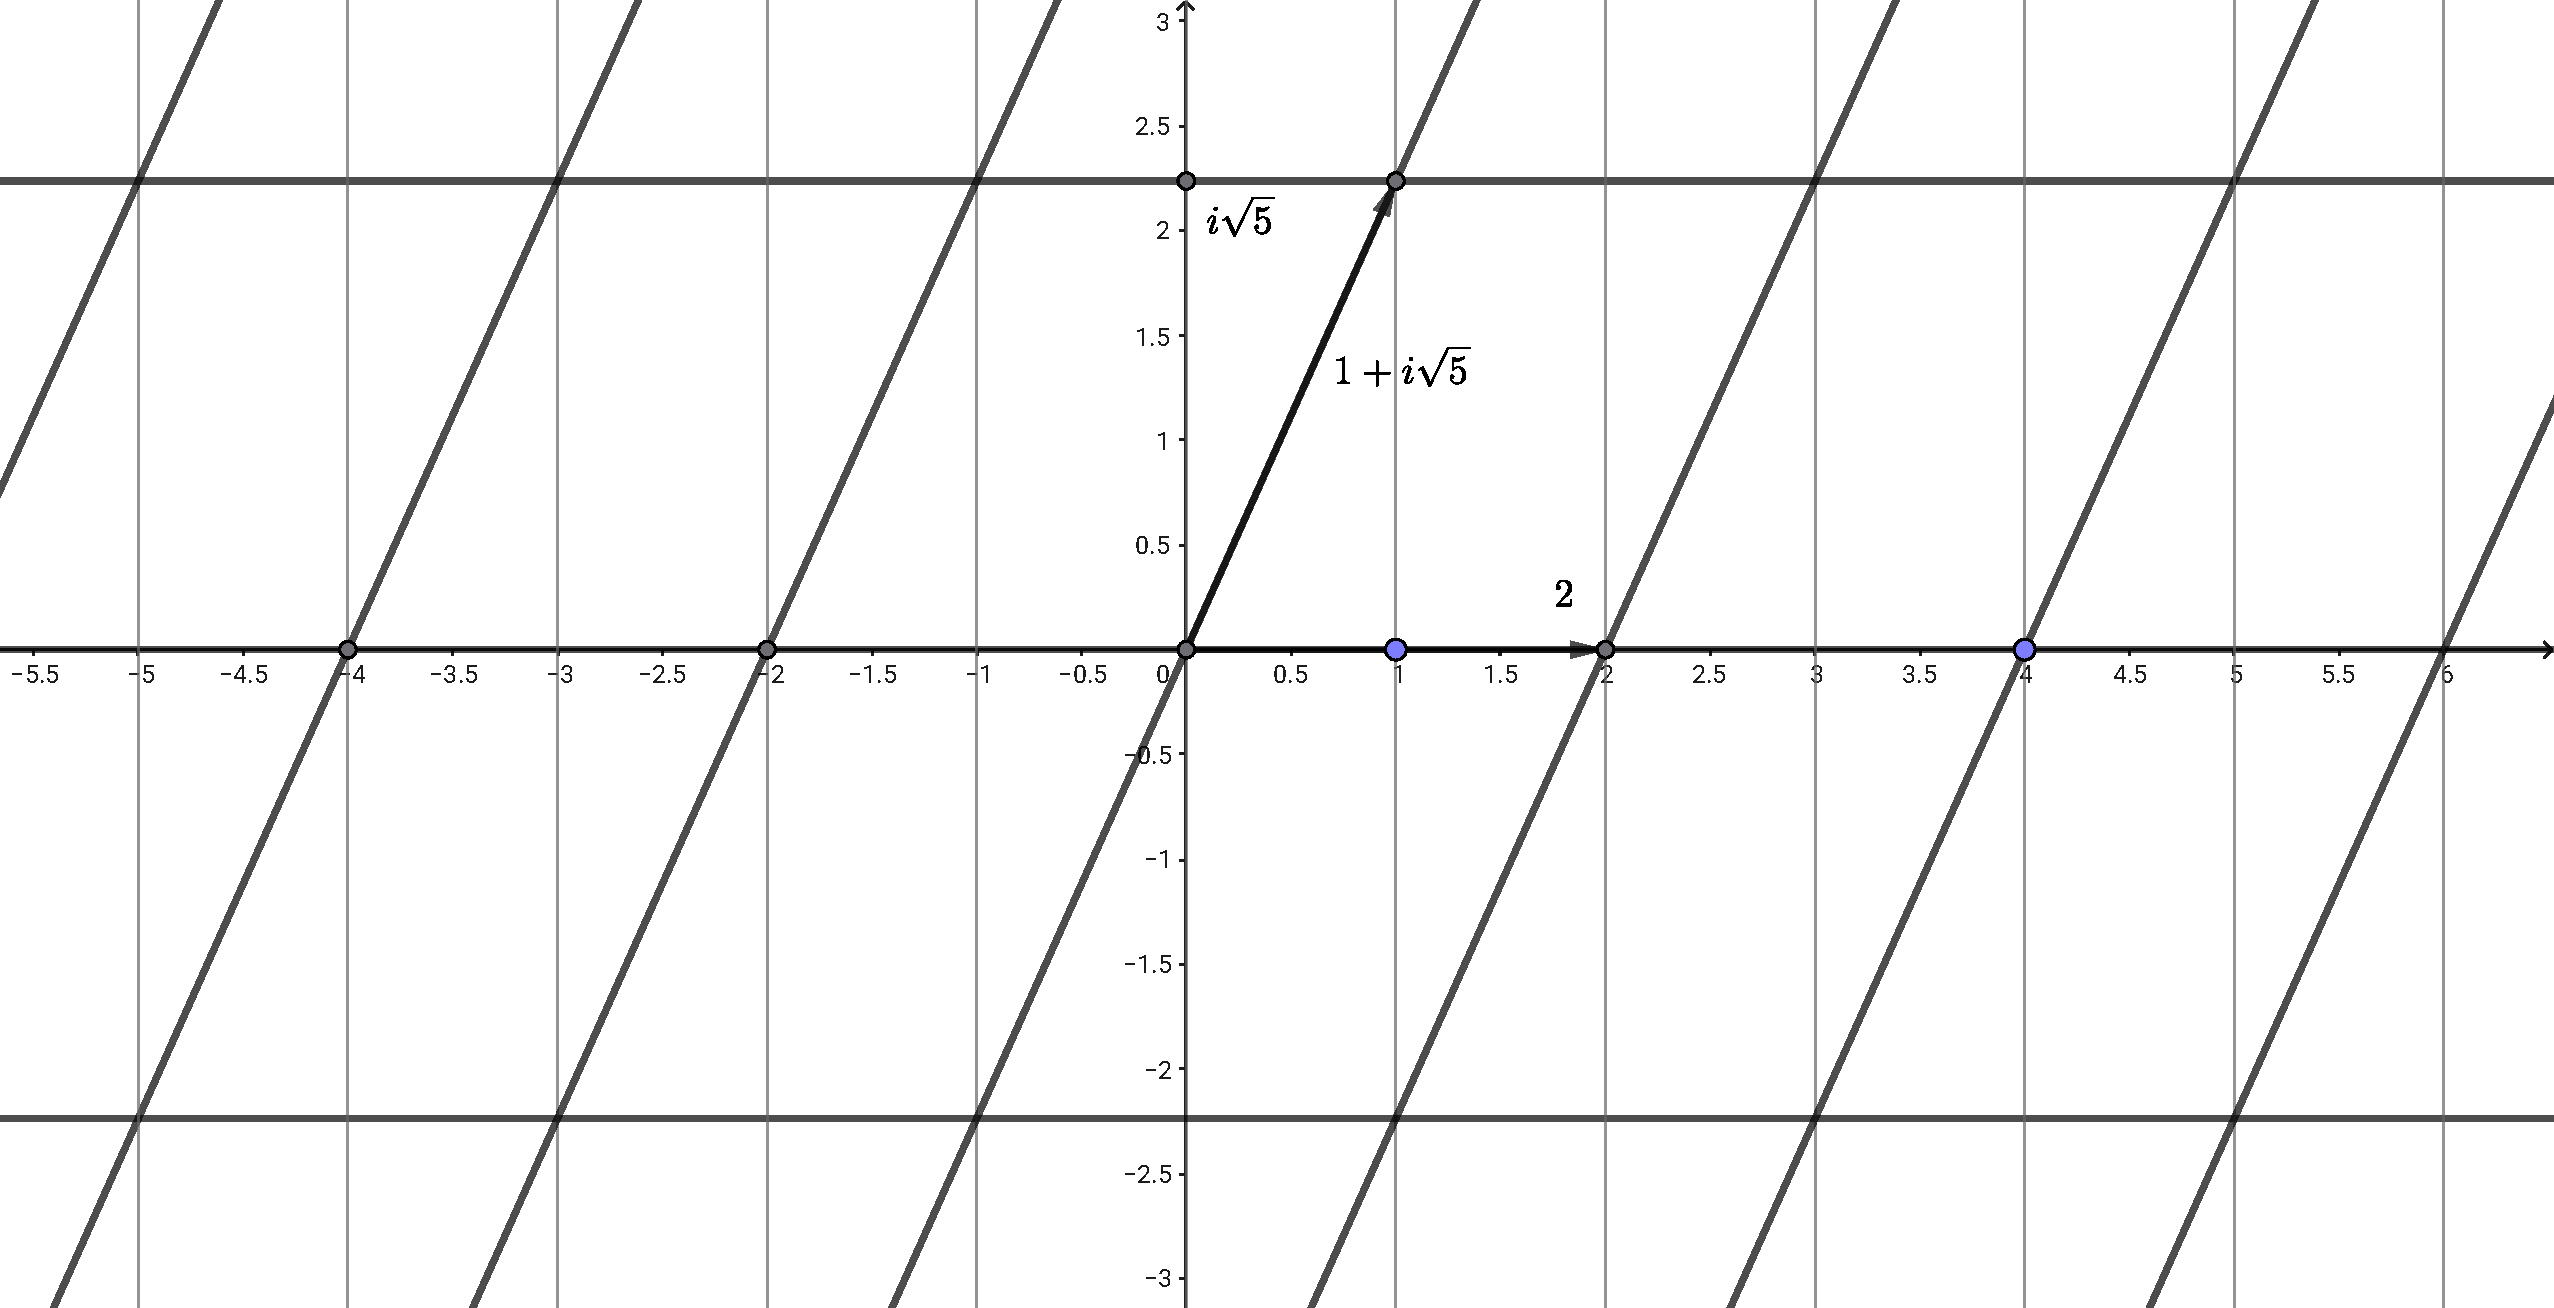
\includegraphics[scale=0.3]{img/ideal-sum}
 \caption{The algebraic integers in $\mathbb{Z}{\sqrt{-5}}$ lie in the gray lattice; the lattice of triangles in black is $(2, 1 + i\sqrt{5})$.}
 \label{fig:ideal-sum}
\end{figure}

For rational integers and Gaussian integers, every ideal is a principal ideal, hence the sum of ideals is also a principle ideal. However, the ideal $A = (2, 1 + i\sqrt{5})$ is \emph{not} a principal ideal. Otherwise assume it is $(\gamma)$, because 2 is in this ideal, hence $\gamma$ divides 2. We've shown previously that 2 cannot be further factorized; it follows that $\gamma$ is either a unit or some associate of 2. Meanwhile, $1 + i\sqrt{5}$ is also in this ideal, hence $\gamma$ divides $1 + i\sqrt{5}$, but $1 + i\sqrt{5}$ cannot be factorized too (see \cref{qn:1-n-delta-irreducible}). It follows that $\gamma$ is either a unit or some associate of $1 + i\sqrt{5}$. In summary, $\gamma$ can only be a unit, but $\pm 1$ isn't in $(2, 1 + i\sqrt{5})$, for otherwise assume:

\begin{align*}
\pm 1 &= 2m + (1 + i\sqrt{5})n &&\text{for integers } m, n \\
  &= 2m + n + ni\sqrt{5}
\end{align*}

Equating the real and imaginary parts:

\begin{align*}
\pm 1 &= 2m + n & n = 0
\end{align*}

It turns out $m = \pm\dfrac{1}{2}$, contradicting with that $m$ is an integer. Therefore, $A = (2, 1 + i\sqrt{5})$ is not a principal ideal, whose lattice is not the shape of rectangles, but triangles as shown in \cref{fig:ideal-sum}. Despite a non-principal ideal, $A$ acts like \enquote{the highest common divisor.} As \enquote{to divide is to contain,} $A$ contains (2), it acts like a divisor of 2; meanwhile, $A$ contains $(1 + i\sqrt{5})$, it also acts like a divisor of $1 + i\sqrt{5}$; therefore, $A$ acts like the highest common divisor of 2 and $1 + i\sqrt{5}$ (analogue to rational integers and Gaussian integers, if the highest common divisor of $a$ and $b$ is $d = (a, b)$, then $(a) + (b) = (d)$).

Even more, $A$ acts like a prime. Let's see how the principal ideal $(p)$ generated by a rational prime $p$ behaves. First of all, a prime $p \ne 1$. Actually the ideal (1) is the set of all integers (see \cref{qn:trivial-ideals}), and indeed, the ideal $(p)$ is not $\mathbb{Z}$ because it does not include 1. Second, $p$ can be divided only by 1 and itself. By \enquote{to divide is to contain,} only ideal (1), namely all integers, and $(p)$ itself contain $(p)$; any other ideal does not contain $(p)$. It's similar for $A$: first, $A$ is identical to (1) as we've shown that $1 \notin A$; second, any other ideal except (1) and $A$ itself does not contain $A$; otherwise, suppose there is some ideal $I$ containing $A$ and $I$ has some element not in $A$, denoted by $\alpha = 2m + 1 + n(1 + i\sqrt{5})$. But altering it to $\alpha - 1 = 2m + n(1 + i\sqrt{5})$, which belongs to $A$; negating it, $1 - \alpha$ also belongs to $A$ (see \cref{qn:zero-in-ideal}). Now $\alpha \in I, 1 - \alpha \in A \subset I$, by the definition of ideal, $\alpha + (1 - \alpha) = 1 \in I$. Therefore, $I = (1)$.

In the same way, one may show that $\overline{A} = (2, 1 - i\sqrt{5})$ acts like a prime. We intent to chose the symbol of conjugation because all numbers in $\overline{A}$ are exactly conjugates to the numbers in $A$. Moreover, we next generate four such ideals from the four divisors of $6 = 2 \times 3 = (1 + i\sqrt{5})(1 - i\sqrt{5})$:

\begin{align*}
A &= (2, 1 - i\sqrt{5})  & \overline{A} &= (2, 1 - i\sqrt{5}) &
B &= (3, 1 - i\sqrt{5})  & \overline{B} &= (3, 1 - i\sqrt{5})
\end{align*}

\index{ideal!product}
Dedekind in 1871 defined the product of two ideals $A$ and $B$ as below:

\[
AB = \{a_1b_1 + a_2b_2 + \dotsb + a_kb_k\}
\]

where $a_1, a_2, \dotsc, a_k \in A, b_1, b_2, \dotsc, b_k \in B$ are elements in each ideal. As such, if an ideal $C = AB$, then the ideal $A$ divides ideal $C$. By Dedekind's definition, the product of principal ideals is again a principal ideal, that is, $(a)(b) = (ab)$. It follows that ideal $(a)$ divides ideal $(ab)$. For example, since $(2)(3) = (6)$, ideal $(2)$ divides ideal $(6)$, which exactly corresponds to the division of rational numbers. If ideal $A$ is generated by $(a, b)$, ideal $B$ is generated by $(c, d)$, then $AB = (ac, ad, bc, bd)$ (see \cref{qn:ideal-product}). Let us next compute the product of $A\overline{A}$:

\index{ideal factorization}
\[
A\overline{A} = (2, 1 + i\sqrt{5})(2, 1 - i\sqrt{5}) = (4, 2 + 2i\sqrt{5}, 2 - 2i\sqrt{5}, 6)
\]

where $4, 6, 2 \pm 2i\sqrt{5}$ all can be divided by 2. By \enquote{to divide is to contain,} the principal ideal $(2)$ contains $A\overline{A}$. Meanwhile, $4 \in A\overline{A}, 6 \in A\overline{A}$, hence $6 - 4 = 2 \in A\overline{A}$. It follows that $(2)$ is contained by  $A\overline{A}$. Therefore, $A\overline{A} = (2)$. In the same way, one may show that $B\overline{B} = (3)$. Next, let us compute the product of $AB$:

\[
AB = (2, 1 + i\sqrt{5})(3, 1 + i\sqrt{5}) = (6, 2 + 2i\sqrt{5}, 3 + 3i\sqrt{5}, (1 + i\sqrt{5})^2)
\]

where each of $6, 2 + 2i\sqrt{5}, 3 + 3i\sqrt{5}, (1 + i\sqrt{5})^2$ can be divided by $(1 + i\sqrt{5})$. By \enquote{to divide is to contain,} the principal ideal $(1 + i\sqrt{5})$ contains $AB$; meanwhile, $3 + 3i\sqrt{5} \in AB, 2 + 2i\sqrt{5} \in AB$, their difference, $1 + i\sqrt{5} \in AB$. It follows that $(1 + i\sqrt{5})$ is contained by $AB$. Therefore, $AB = (1 + i\sqrt{5})$. In the same way, one may show that $\overline{AB} = (1 - i\sqrt{5})$. Put these all together:

\[
(6) = (2)(3) = (A\overline{A})(B\overline{B}) = (AB)(\overline{AB}) = (1 + i\sqrt{5})(1 - i\sqrt{5})
\]

Thus Dedekind saves the unique factorization. $(6)$ is uniquely factorized to $A\overline{A}B\overline{B}$.

\section{Infinite numbers}

\index{Galileo's paradox}
Our journey of numbers is gradually coming to the end. Along it, we've explored natural number, zero, integers, rational and irrational numbers, the continuum of real numbers, complex numbers, and algebraic numbers. Some are contained by others, for instance, natural numbers are part of integers; some are mutually exclusive, like the rational and irrational numbers. It's natural to ask which ones are more numerous? Are the numbers commonly in daily life more abundant while the rare ones fewer? Our experiences are not always true; our intuition some times is unreliable. The difficulty of these problems is that, all these are infinite sets except for zero. How big is infinity? Intuitively, it is as large as can be. But then how can we compare infinities? One may argue that even numbers are only half as many as integers, hence are fewer than integers. However, doubling any integer yields an even number, and dividing any even number by 2 gives an integer. From this perspective, every integer corresponds to a even number, so the two sets seem to be equally large. Which argument is correct? Galileo, father of the modern science, made a paradox in his scientific work \emph{Two New Sciences} in 1636: Some numbers are squares, while others are not; therefore, all the numbers, including both squares and non-squares, must be more numerous than just the squares. And yet, for every number there is exactly one square, which forms the sequence $1, 4, 9, 16, 25, \dotsc$ hence, there cannot be more of one than of the other. This paradox is known as Galileo's paradox. Besides numbers, there are similar paradoxes in Geometry. For instance, \cref{fig:circles-paradox} shows two circles at the same centre; every radius connects two points in each circle, which is one to one correspondence between them. There seems to be the same amount of points in each circle. But in our common sense, there seems to be more points in the bigger circle than the smaller one. Galileo thus concluded that the ideas of less, equal, and greater couldn't apply to infinite things like natural numbers, hence rejected term of \enquote{all} the natural numbers.

\begin{figure}[htbp]
 \centering
   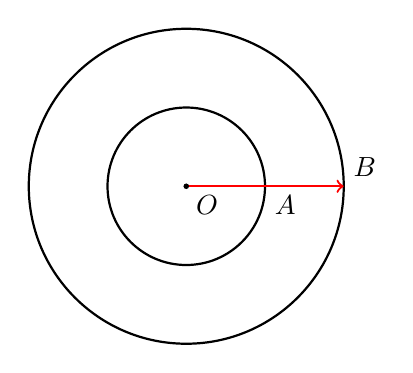
\begin{tikzpicture}[
       scale=0.5,
       circle_style/.style={draw, black, thick},
       radius_style/.style={draw, red, thick, ->}
   ]

   \draw[circle_style] (0,0) circle (2cm);

   \draw[circle_style] (0,0) circle (4cm);

   \draw[radius_style] (0,0) -- (4,0);

   \fill[black] (0,0) circle (2pt);
   \node[below right] at (0,0) {$O$};
   \node[below right] at (2,0) {$A$};
   \node[above right] at (4,0) {$B$};

   \end{tikzpicture}

 \caption{Every point in the big circle corresponds to a point in the small circle.}
 \label{fig:circles-paradox}
\end{figure}

\index{infinite set} \index{one to one correspondence}
About two hundred years after Galileo, Georg Cantor considered these paradoxes again. He realized the idea in our common sense that a part must be smaller than the whole, isn't necessarily true. If accept the opposite notion that a part can be as large as the whole, although counter-intuitive, then the problem would be solved. Cantor defines two sets be equinumerous -- of the same size (cardinal number) or have same number of elements -- if there is one-to-one correspondence between them. This definition is obviously true for finite sets; when extending to infinite sets, it means there are same amount of even numbers and integers! and same amount of squares and natural numbers; same amount of points in two circles... Dedekind, gave such a definition of infinite set in 1888: if some proper subset of a set is equinumerous to this set, then it is a infinite set\cite{Dedekind-1858}.

\index{Hilbert's Grand hotel}
To explain Cantor's idea, Hilbert told an interesting story in a lecture in 1924 (published in 2013). It was later popularized by George Gamow in 1947 through his book \emph{One Two Three... Infinity}. In this story, there was a Grand hotel with infinitely many rooms. It was fully occupied during the hot season. One evening, a tired driver, after passing many \enquote{No vacany} hotels, came to see if there might nonetheless be a room for him. The clerk said: \enquote{No problem, we can make a room for you.} He moved the guest in room 1 to room 2, then moved the guest in room 2 to room 3, and moved the guest in room 3 to room 4, ... He moved every one to the next room. That freed up the first room for this new guest.

The story goes on. On the second day, there came a group of infinitely many guests. The clerk said: \enquote{No problem, we can make rooms for everyone.} He moved the new guest who was in room 1 last night to room 2, then moved the guest in room 2 to room 4, and moved the guest in room 3 to room 6, ... He moved every one from room $i$ to room $2i$. Since the hotel had infinitely many rooms, after moving, room 2, 4, 6, ... these even number rooms were occupied with the guests accommodated yesterday, while the room 1, 3, 5, ... these odd number rooms were freed up. There were infinitely many odd numbers rooms that could accommodate everyone. The story does not end. On the third day, there came infinitely many groups of infinitely many guests each. Could the magic Hilbert's hotel accommodate them all?

\begin{figure}[htbp]
 \centering
 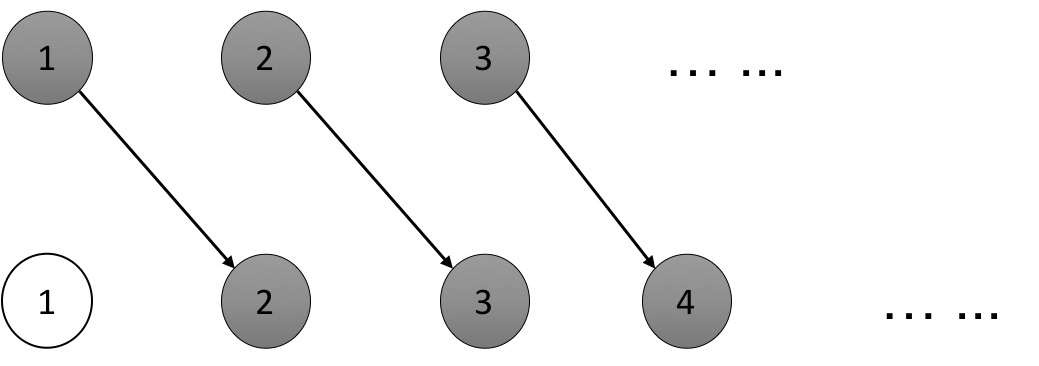
\includegraphics[scale=0.4]{img/Hilbert-hotel-1}
 \caption{First day of Hilbert's Grand hotel}
 \label{fig:Hilbert-hotel-1}
\end{figure}

As shown in \cref{fig:Hilbert-hotel-1}, on the first day, the clerk moved every guest to the next room to free up room 1. Essentially, he established a 1-to-1 correspondence for shadowed circles between the two rows as $n \leftrightarrow n+1$. More over, Hilbert's grand hotel can accommodate $k$ new guests by repeating this arrangement $k$ times.

\begin{figure}[htbp]
 \centering
 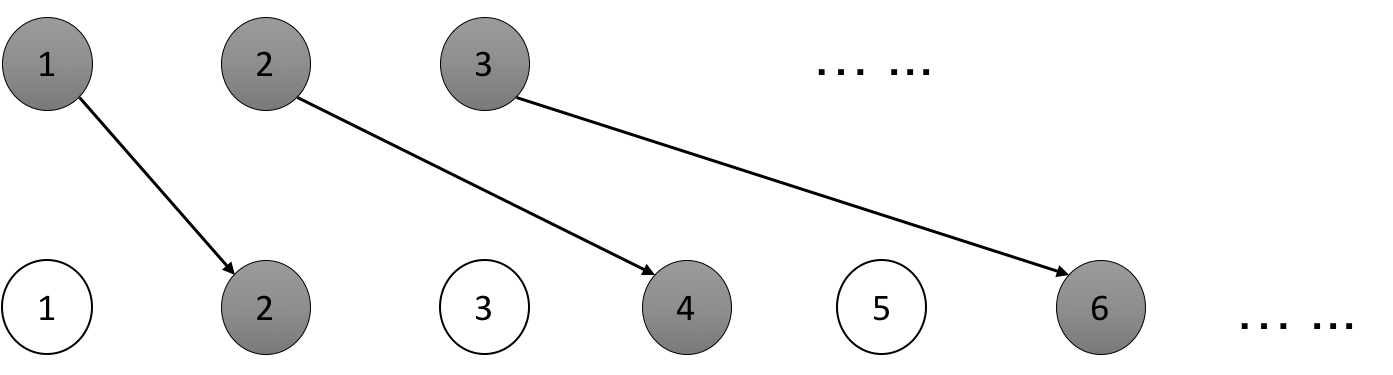
\includegraphics[scale=0.4]{img/Hilbert-hotel-2}
 \caption{Second day of Hilbert's Grand hotel}
 \label{fig:Hilbert-hotel-2}
\end{figure}

\Cref{fig:Hilbert-hotel-2} shows the solution to the second day. The clerk essentially established 1-to-1 correspondence between natural numbers and even numbers, thus freed up infinitely many odd-numbered rooms. Then he established another 1-to-1 correspondence between these empty rooms and infinitely many new guests, which was exact the 1-to-1 correspondence between odd numbers and natural numbers. To solve the problem on the third day, we need think about how to establish 1-to-1 correspondence between (a) the infinitely many groups of infinity many guests, and (b) the infinity many rooms. One may come to the idea to arrange the guests of the first group to room 1, 2, 3, ... then arrange the guests of the second group to room $\infty + 1, \infty + 2, \dotsc$ However, it does not work when considering the arranging process: the first guest of the second group can never know when the first group completes accommodating, hence has no way to determine which room to check in. In contrast on the first day, the new guest immediately knew room 1 is OK for him after the original guest moved to room 2 even though the entire accommodating process is endless. Same situation happened on the second day: when the original guest in room 1 moved to room 2, the first new guest could move to room 1 immediately. Next, after the guest in room 2 moved to room 4 and the guest in room 3 moved to room 6, then the second new guest could move to room 3...

\begin{figure}[htbp]
\centering
\begin{tikzpicture}
  \draw[step=1, very thin, gray] (0, 0) grid (5, 5);
  \draw[->] (-0.25, 0) -- (6, 0) coordinate (x axis);
  \draw[->] (0, -0.25) -- (0, 6) coordinate (y axis);
  \foreach \x in {0, 1, 2, 3, 4, 5}
    \path (\x, -0.25) node[left] {\x};
  \foreach \y in {1, 2, 3, 4, 5}
    \path (-0.25, \y) node[below] {\y};
  \foreach \i / \x / \y in {0/0/0, 1/1/0, 2/0/1, 3/0/2, 4/1/1, 5/2/0, 6/3/0, 7/2/1, 8/1/2, 9/0/3, 10/0/4}{
    \path (\x, \y) coordinate (N\i);
    \fill (N\i) circle (1pt) node[above right=3pt of N\i] {\i};
  }
  \foreach \i in {0,...,9} {
    \pgfmathsetmacro{\j}{\i+1}
    \draw[-latex, thick] (N\i) to (N\j);
  }
\end{tikzpicture}
\caption{One solution to number the infinity of infinity}
\label{fig:NNtoN}
\end{figure}

\Cref{fig:NNtoN} gives a numbering solution. For convenient, for each group, label the first guest 0, the second guest 1, the third guest 2, ...; label the guests already accommodated in the hotel as group 0, the first group of guest as group 1, the second group of guest as group 2, ... In this figure, every guest corresponds to a grid point. We also label the hotel rooms beginning from 0. Now we arrange rooms in this order: assign the guest 0 of group 0 to room 0, the guest 1 of group 0 to room 1, the guest 0 of group 1 to room 2, the guest 0 of group 2 to room 3, the guest 1 of group 1 to room 4, ... Along the zig-zag path, assign rooms one by one, without missing any guests, hence establish a 1-to-1 correspondence between every guest in infinitely many groups and the infinity many rooms. Hilbert's Grand hotel surprisingly holds \enquote{two-dimensional} infinity\footnote{The traditional solution uses the Euclid's theorem, that there are infinitely many prime numbers. Empty the odd numbered rooms by sending the guest in room $i$ to room $2^{i}$, then put the first group's guests in rooms $3^{n}$, the second group's guests in rooms $5^{n}$, ... put the $k$-th group's guests in rooms $p^n$, where $p$ is the $k$-th prime number. This solution leaves certain rooms empty, specifically, all odd numbers that are not prime powers, such as 15 or 847, will no longer be occupied.}.

\subsection{One-to-one correspondence and infinite set}

Hilbert's Grand hotel shows the set of natural numbers is equinumerous with its proper subsets like even/odd numbers. And the sets of one dimensional natural number $n$ and two dimensional pair $(m, n)$ are also equinumerous. Starting from natural numbers, one may extend a series of infinite sets through 1-to-1 correspondence.

\begin{enumerate}[(1)]
\item \textbf{Integers}. Establish the following 1-to-1 correspondence:

\begin{tabular}{ccccccccc}
0 & 1 & -1 & 2 & -2 & ... & $n$ & $-n$ & ... \\
$\updownarrow$ & $\updownarrow$ & $\updownarrow$ & $\updownarrow$ & $\updownarrow$ & & $\updownarrow$ & $\updownarrow$ & \\
0 & 1 &  2 & 3 &  4 & ... & $2n - 1$ & $2n$ & ... \\
\end{tabular}

It extends natural numbers to integers, where the odd natural numbers correspond to positive integers and even natural numbers correspond to negative integers and zero. The set of integers is as infinite as the set of natural numbers.

\item \textbf{Rational numbers}. Express every rational number as $p/q$, where $q \ne 0$. Analog to the story of Hilbert's Grand hotel on the third day, which established 1-to-1 correspondence between pairs of $(p, q)$ and natural numbers. We adjust it to rational numbers of $p/q$. Put negative numbers aside for now, we skip whenever $q$ is zero or $p/q$ is reducible (with some common divisor greater than 1). Then we re-use the correspondence in (1) to cover negative rational numbers. In this way, we construct rational numbers from natural numbers as shown in below table:

\begin{tabular}{cccccccccc}
0 & 1 & 2 & 3 & 4 & 5 & 6 & 7 & 8 & ... \\
$\updownarrow$ & $\updownarrow$ & $\updownarrow$ & $\updownarrow$ & $\updownarrow$ & $\updownarrow$ & $\updownarrow$ & $\updownarrow$ & $\updownarrow$ & \\
0 & 1 & $\dfrac{1}{2}$ & $-\dfrac{1}{2}$ & -1 & -2 & $-\dfrac{2}{3}$ & $-\dfrac{1}{3}$ & $\dfrac{1}{3}$ & ... \\
\end{tabular}

This shows the set of natural numbers is as infinite as the set of rational numbers.

\index{algebraic numbers}
\item \textbf{Algebraic numbers} are roots of the algebraic equations:

\[
a_0 x^n + a_1 x^{n-1} + \dotsb + a_n = 0
\]

where $a_0 \ne 0, a_1, \dotsc, a_n$ are integers. Define the positive integer:

\[
h = n + |a_0| + |a_1| + ... + |a_n|
\]

which is the sum of the degree and coefficients. We call $h$ the height of the equation. Given any equation, $h$ is a definitive natural number; conversely, given a height $h$, there can be multiple equations. For example, the height of equations $x - 3 = 0$, $x^3 + 1 = 0$, $x^3 - 1 = 0$, $x^2 + x + 1 = 0$, and $x^2 - x + 1 = 0$ are all 4. Nevertheless, there are finitely many equations for every $h$, therefore, one may enumerate all equations in this way: first list all equations of height $h=1$, then list the equations of height $h=2$, ... and repeat. The equations with the same heights can be list in arbitrary order. By the fundamental theorem of algebra, the number of roots equals the degree $n$. If taking the duplicated roots into account, then the distinct ones are not more than $n$. To list all algebraic numbers, first enumerate the roots of the equations with height $h=1$ ($x = 0$ is the only such equation, which has 0 as the single root); then enumerate the roots of the equations with height 2. As different equations may share some same root, we skip those if have appeared. In this way, we establish 1-to-1 correspondence between algebraic numbers and natural numbers. It shows the set of algebraic numbers is as infinite as the set of natural numbers.
\end{enumerate}

\subsection{Countable and uncountable infinity}
\index{countable infinite set}
We have a problem next: can we extend natural numbers to real numbers, including transcendental numbers like $\pi$ and $e$? Through 1-to-1 correspondence, we extend from natural numbers to integers, rationals, and algebraic numbers (including irrational numbers like radicals). The existence of 1-to-1 correspondence between them shows they are equinumerous. A set is called \emph{countable} infinite if it has the same cardinality as the set of natural numbers. Are all infinite sets countable? Are there any larger infinities? Cantor, on 29th November 1873, wrote to Dedekind about this problem, \enquote{take the set of all natural numbers $n$ and denote it $\mathbb{N}$. Further, consider, say, the set of all positive real numbers $x$ and denote it $\mathbb{R}$. Then the question is simply this: can $\mathbb{N}$ be paired with $\mathbb{R}$ in such a way that to every individual of one set corresponds to one and only one individual of the other? At first glance, one says to oneself, \enquote{No, this is impossible, for $\mathbb{N}$ consists of discrete parts and $\mathbb{R}$ is a continuum.} But nothing is proved by this objection. And much as I too feel that $\mathbb{N}$ and $\mathbb{R}$ do not permit such a pairing, I still cannot find the reason. And it is this reason that bothers me; maybe it is very simple.}

\index{diagonal argument}
One week after on 7th December, Cantor wrote again to Dedekind, telling that he proved it was impossible to establish 1-to-1 correspondence between natural numbers and real numbers, hence real numbers are uncountable. This was the day that set theory born. Cantor had given two proofs, the second one is the renowned {\em diagonal argument}. Assume for contradiction that the real numbers in $(0, 1)$ are countable, so there exits 1-to-1 correspondence to natural numbers. List all real numbers in this interval in decimals, as $a_0, a_1, a_2, \dotsc, a_n, \dotsc$. For irrationals, their decimals are endless non-repeating; for rationals, their decimals may either repeat, for instance, $\dfrac{1}{3} = 0.333...$, or finite that can be turned into repeating by lemma \ref{th:cycle-of-9}, for example:$\dfrac{1}{2} = 0.5 = 0.4999\dotsm$. List all reals in $(0, 1)$ as below:

\begin{align*}
a_0 &= 0.a_{00}a_{01}a_{02}a_{03}\dotsm\\
a_1 &= 0.a_{10}a_{11}a_{12}a_{13}\dotsm\\
a_2 &= 0.a_{20}a_{21}a_{22}a_{23}\dotsm\\
a_3 &= 0.a_{30}a_{31}a_{32}a_{33}\dotsm\\
    &\dotso \\
a_n &= 0.a_{n0}a_{n1}a_{n2}a_{n3}\dotsm\\
    &\dotso
\end{align*}

Note $a_0, a_1, a_2, \dotsc$ are not necessarily ascending. Cantor next constructs a number $b = 0.b_0b_1b_2b_3 \dotsm b_n \dotsm$, where the $n$-th digit $b_n \neq a_{nn}$. To do this, if $a_{nn} \neq 5$, then let $b_n = 5$, else let $b_n = 6$. The constructed number $b$ can't equal any number in above list for it differs from the $n$-th digit of the $n$-th number at least, that is, the diagonal digits are different as shown in bold below:

\begin{align*}
a_0 &= 0.\pmb{a_{00}}a_{01}a_{02}a_{03}\dotsm \\
a_1 &= 0.a_{10}\pmb{a_{11}}a_{12}a_{13}\dotsm \\
a_2 &= 0.a_{20}a_{21}\pmb{a_{22}}a_{23}\dotsm \\
a_3 &= 0.a_{30}a_{31}a_{32}\pmb{a_{33}}\dotsm \\
    &\dotso \\
a_n &= 0.a_{n0}a_{n1}a_{n2}a_{n3} \dotsm \pmb{a_{nn}}\dotsm \\
    &\dotso
\end{align*}

However, we assume all real numbers in $(0, 1)$ are list without missing. As $0 < b < 1$, which should be included in the list, but it does not equal any $a_i$, a contradiction. It shows impossible to establish 1-to-1 correspondence between real numbers and natural numbers. One may argue why can't add $b$ to the list of $a_0, a_1, a_2, \dotsc$? Suppose after adding $b$ to the list, its position is the $m$-th number, we then construct another new number $c$, where its $m$-th digit does not equal $b_m$. Therefore, it's another number not being included.

\index{uncountable infinite set}
Cantor's proof shows a surprising result: the set of real numbers in $(0, 1)$ is uncountable! It is more numerous than the set of natural numbers. Courant and Robbins give a geometric proof in \emph{What is mathematics}. Assume the points in the unit line segment $(0, 1)$ can be enumerated as $a_1, a_2, a_3, ...$ Cover point $a_1$ by an interval of length 1/10, cover point $a_2$ by an interval of length 1/100, ... cover point $a_n$ by an interval of length $1/10^n$, and so on. It follows that the unit line segment (0, 1) is completely covered (with overlaps) by these sub-intervals of length 1/10, 1/100, 1/1000, ... However, the total length of these sub-intervals, which is the sum of a geometric series, is $1/10 + 1/100 + 1/1000 + \dotsb = 1/9 < 1$. It is impossible to cover the line segment of length 1 by intervals of total length 1/9, a contradiction. It shows the points in the line segment are uncountable\cite{Courant1969}.

As the next step, establish 1-to-1 correspondence: $y = \pi x - \frac{\pi}{2}$. It sends every real number in $(0, 1)$ to $(-\frac{\pi}{2}, \frac{\pi}{2})$ without any missing. We immediately conclude that the real numbers in this new interval are uncountable. Finally, establish another 1-to-1 correspondence: $ y = tan(x)$. It sends every real number between $-\frac{\pi}{2}$ and $\frac{\pi}{2}$ to the set of all real numbers without any missing. There is another geometric solution to establish 1-to-1 correspondence between the unit line segment and real numbers. Bend the line segment to a semicircle of length 1, then draw an infinite line $L$ outside the circle. From any point $P$ in $L$, connect it with the centre of the circle, it intersects with the arc at a point $Q$, as in \cref{fig:seg-to-line}. Cantor therefore concluded the set of real numbers was not countable. It is a higher level of infinity than countable sets, namely the uncountable infinite set.

\begin{figure}[htbp]
 \centering
 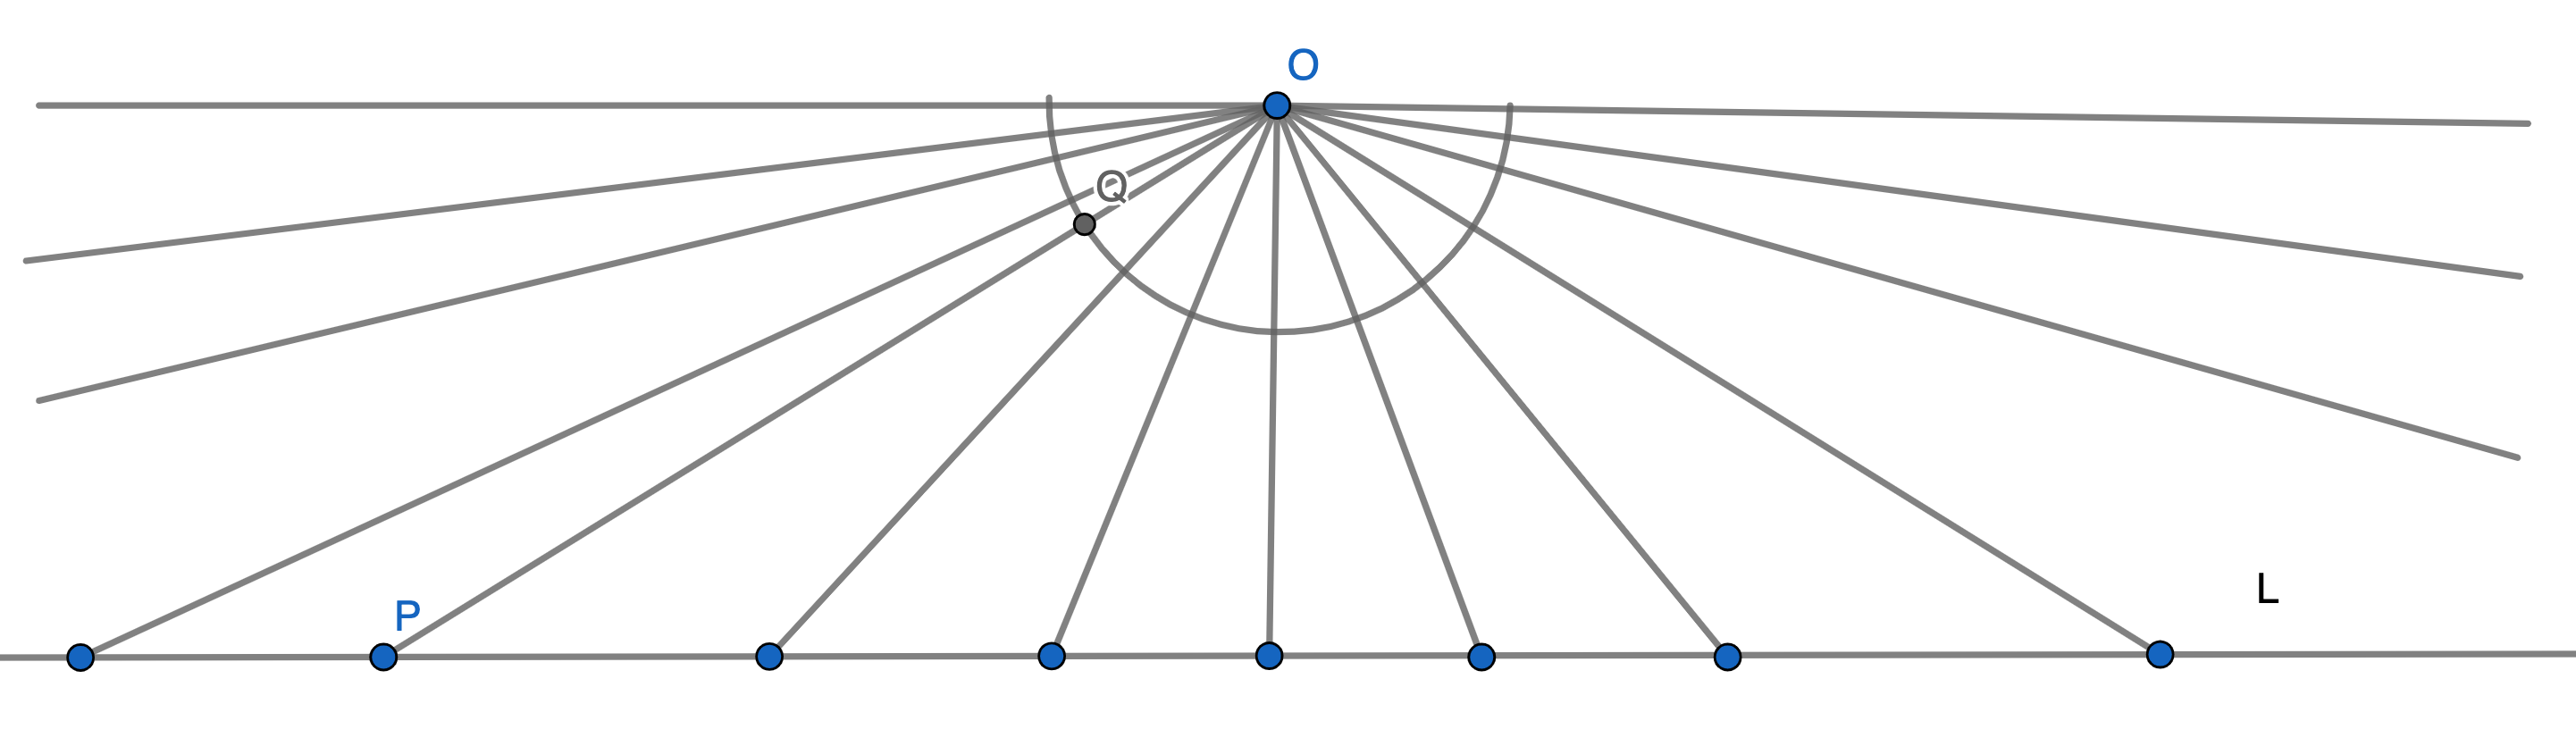
\includegraphics[scale=0.6]{img/seg-to-line}
 \caption{map a semicircle of length 1 to all real numbers.}
 \label{fig:seg-to-line}
\end{figure}

\index{Continuum hypothesis}
In Euclid's {\em Elements}, \enquote{a point is that which has no part.}, and line consists of points. There are irrational numbers in the line, in other words, rationals can't fully cover a line, while real numbers can. The above proof shows the points in the unit line segment, the points in a line segment of any length, and the points in infinitely long line, for instance, the number line, they are all uncountable infinite sets of the same cardinality. So as the points in circles at the same centre. Comparing rationals and irrationals, for any two distinct rational numbers, there are infinitely many irrational numbers in between; for any two distinct irrational numbers, there are also infinitely many rational numbers in between. Although seems same, by Cantor's theory, rational numbers are countable, but irrational numbers are uncountable. Irrationals are more numerous than rationals. Further, we've seen that algebraic numbers are countable, but the transcendental numbers like $\pi$ and $e$, are uncountable, hence more numerous than algebraic numbers. Cantor did not stop but went on considering if exists any infinite set that between countable infinite set like natural numbers and uncountable infinite set like continuum of reals. This led to the conjecture of continuum hypothesis in 1878. He tried for many years but was unable to prove it. Continuum hypothesis became the first on Hilbert's list of 23 important open questions that was presented at ICM in 1900 in Paris. Through the work of Gödel and Paul Cohen, it was proven in 1963 that the continuum hypothesis is independent of the axiomatic set theory system. This implies that one can neither prove nor disprove the continuum hypothesis within set theory.

\begin{figure}[htbp]
 \centering
 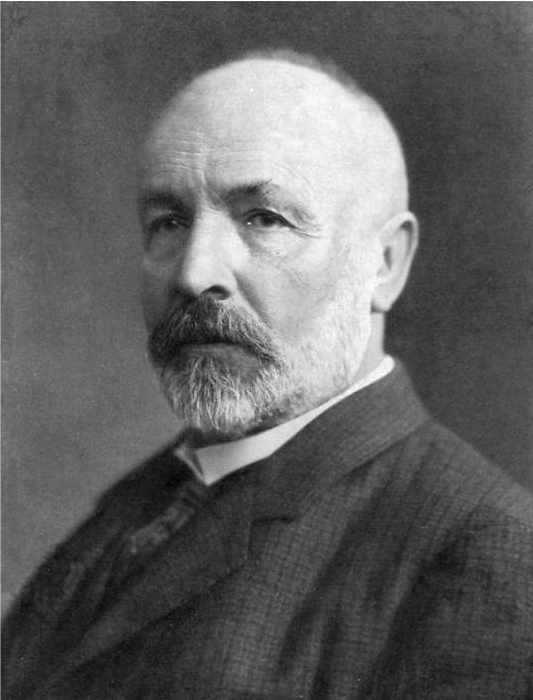
\includegraphics[scale=0.5]{img/Cantor}
 \caption{Georg Cantor, 1845 - 1918}
 \label{fig:Cantor}
\end{figure}

\begin{mdframed}
\index{Cantor}
Georg Cantor (\cref{fig:Cantor}) was the founder of set theory. He was born in 1845 in the western merchant colony of Saint Petersburg, Russia, and brought up in the city until he was eleven. His father was a successful merchant, and member of the Saint Petersburg stock exchange; his mother came from a family well-known of music. When his father became ill, the family moved to Germany Frankfurt in 1856. Cantor demonstrated exceptional skill in mathematics in school. But his father wanted Cantor to became \enquote{a shining star in the engineering firmament}. However, at the age of 17, Cantor had sought his father's permission to study mathematics at university and he was overjoyed when eventually his father consented\cite{HanXueTao16}.

He entered the Polytechnic of Zürich in 1862, then moved to the University of Berlin in 1863. He attended lectures by Leopold Kronecker, Karl Weierstrass and Ernst Kummer. He spent the summer of 1866 at the University of Göttingen. Cantor was a good student, and he received his doctorate degree in 1867 with the dissertation on number theory. Cantor later took up a position at the University of Halle, where he spent his entire career.

At that time, many mathematicians were trying to rebuild the rigorous logical foundation of analysis led by Weierstrass. Cantor was also influenced by this movement. He soon realized the importance to study real numbers as the basis of calculus, which became the beginning of set theory research. In 1872, he met and began a friendship with the young mathematician Richard Dedekind while on holiday in Switzerland. Even in Cantor's honeymoon in Harz mountains, Cantor spent much time in mathematical discussions with Dedekind. They started a long time correspondence between each other.

In 1874, Cantor published his first revolutionary paper about set theory at the age of 29. It marked as the beginning of set theory as a branch of mathematics. With the extraordinary ingenuity, Cantor established set theory in the following ten years almost alone, leading the revolution of infinity in mathematics. However, he was not well recognized during his most creative period. He desired, but was not able to obtain a professor chair at the University of Berlin. He spent his career at the University of Halle, which was a infamous university with a meager salary. Cantor's theory was originally regarded as so counterintuitive – even shocking. People found paradoxes hidden in infinity sets (see Russell's paradox in next chapter). Cantor's work encountered resistance from mathematical contemporaries. Among them, some were famous mathematicians, including his teacher, the leading mathematician in Berlin, Leopold Kronecker. He had a famous saying: \enquote{God made the integers, all else is the work of man.} He objected to Cantor's theory about infinity and transfinite numbers, said it was not mathematics but mysticism. Mathematics was headed for the madhouse under Cantor. Henri Poincaré referred to Cantor's work as a \enquote{disease} from which mathematics would eventually be cured. Poincaré said, \enquote{There is no actual infinite; the Cantorians have forgotten this, and that is why they have fallen into contradiction.} Later Hermann Weyl criticized Cantor's hierarchy of infinities as \enquote{fog on fog}. Hermann Schwartz was originally a friend of Cantor, but he stopped the correspondence with Cantor as opposition to Cantor's ideas continued to grow.

The tragedy was not the set theory, but Cantor went to the madhouse. Cantor suffered his first known bout of depression in May 1884. During the rest of his life, the depression recurred several times with different intensity, driving him from the community into the mental hospital refuge.
%% In 1904 he was agitated by a paper presented by Julius König at the Third International Congress of Mathematicians. The paper was read in front of his daughters and colleagues. Cantor was shaken, and sent to hospital again.
Cantor retired in 1913, living in poverty (because of the war conditions). In June 1917, he entered the sanatorium for the last time and continually wrote to his wife asking to be allowed to go home. Cantor died on January 6, 1918, in the sanatorium where he had spent the last year of his life.

Cantor's set theory was publicly acknowledged and praised at the first ICM held in Zurich in 1897. Adolf Hurwitz (1859 - 1919) openly expressed his great admiration of Cantor and proclaimed him as one by whom the theory of functions has been enriched. Jacques Hadamard expressed his opinion that the notions of the theory of sets were known and indispensable instruments. Over time, people gradually realized the importance of set theory. Hilbert praised Cantor's work as \enquote{the finest product of mathematical genius and one of the supreme achievements of purely intellectual human activity.}
\end{mdframed}

\begin{Exercise}[label={ex:algebraic}]
\Question{Assume $x^n + y^n = z^n$, show that if any two of $x, y, z$ has a common divisor $d$, then it is also a divisor of the third. \label{qn:xyz-coprime}}

\Question{Show that if there is a rational root to the monic equation $x^n + a_{n-1} x^{n-1} + \dotsb + a_1 x + a_0 = 0$, then this root is integral. \label{qn:rational-solution-is-integral}}

\Question{Show that the norm is multiplicative. \label{qn:norm-is-multiplicative}}

\Question{Explain why the norm of a quadratic integer is the constant term of the corresponding quadratic equation. \label{qn:quadratic-norm}}

\Question{If $a, b$ are relatively prime, show that the conjugate quadratic integers $a \pm bi\sqrt{m}$ are relatively prime. \label{qn:coprime-of-conjugates}}

\Question{By the definition of norm in conjugates, show that the norm of Eisenstein integer is $a^2 - ab + b^2$. \label{qn:norm-of-z-omega}}

\Question{Show that the norm of Eisenstein integers can not be negative.}

\Question{What are the units of Eisenstein integers?}

\Question{Draw the lattice of Eisenstein integers of $\rho \beta$.}

\Question{Using lattice, show that the Euclidean algorithm exists for Eisenstein integers.}

\Question{Show that $1 \pm i\sqrt{5}$ cannot be further factorized. \label{qn:1-n-delta-irreducible}}

\Question{Show that the sum of ideals is an ideal. \label{qn:sum-of-ideals}}

\Question{For the parent set $R$ of an ideal, suppose 0 and 1 are in it, and for any element $y$ in $R$, its negative, $-y$ is also in $R$. Prove for any ideal of $R$, (1) 0 is in the ideal; (2) if $a$ is in the ideal, then $-a$ is in the ideal. \label{qn:zero-in-ideal}}

\Question{(0) is called zero ideal, (1) is called unit ideal, what elements are in them respectively? \label{qn:trivial-ideals}}

\Question{Verify that if ideal $A = (a, b) = \{ax + by | x, y \in R\}$ and ideal $B = (c, d)$, then their product $AB = (ac, ad, bc, bd)$. \label{qn:ideal-product}}

\Question{We establish 1-to-1 correspondence between rooms and guests as shown in \cref{fig:NNtoN}. Which room is the guest $j$ of group $i$ checked in? Conversely, which guest of which group is checked in room $k$? }

\Question{There are other solutions to the story of Hilbert's Grand hotel on the third day. \Cref{fig:PWW-NNtoN} shows the cover page of \emph{proof without word}. Give a numbering scheme based on this figure.
\begin{figure}[htbp]
 \centering
 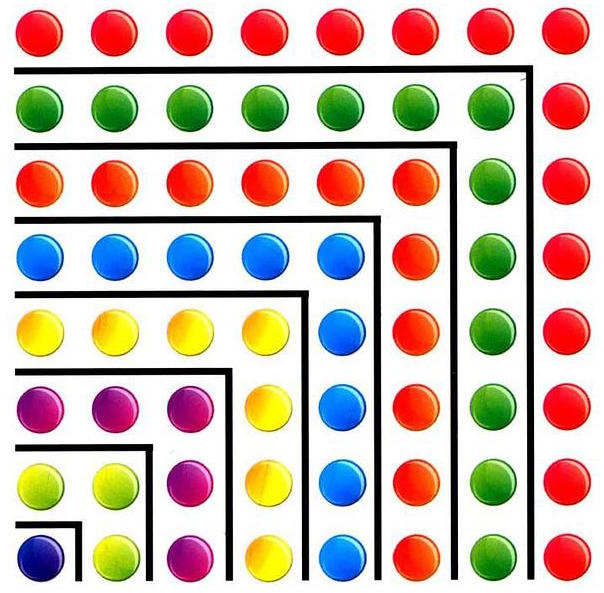
\includegraphics[scale=0.18]{img/PWW}
 \caption{From cover page of \emph{Proof without word}}
 \label{fig:PWW-NNtoN}
\end{figure}
}

\end{Exercise}

\begin{Answer}[ref={ex:algebraic}]
\Question{Assume $x^n + y^n = z^n$, show that if any two of $x, y, z$ has a common divisor $d$, then it is also a divisor of the third.

\begin{proof}
First prove a lemma: if $a^n$ divides $b^n$, then $a$ divides $b$. By fundamental theorem of arithmetic, write $a, b$ as the product of powers of primes:

\begin{align*}
a &= p_1^{a_1}p_2^{a_2}\dotsm p_k^{a_k} & b &= p_1^{b_1}p_2^{b_2}\dotsm p_k^{b_k} q_1^{c_1}q_2^{c_2} \dotsm q_m^{c_m}
\end{align*}

where $p_i$ are prime factors of $a$ and $a_i > 0$. Some of these prime factors appear in $b$, some do not, therefore, $b_j \geq 0$ (0 means the factor does not appear in $b$). $q_j$ are factors only in $b$, hence $c_j > 0$. Raise to $n$-th powers for $a, b$.

\begin{align*}
a^n &= p_1^{a_1n}p_2^{a_2n}\dotsm p_k^{a_kn} & b^n &= p_1^{b_1n}p_2^{b_2n}\dotsm p_k^{b_kn} q_1^{c_1n}q_2^{c_2n} \dotsm q_m^{c_mn}
\end{align*}

As $a^n$ divides $b^n$, it follows that $a_in \leq b_in$, divided by $n$ gives $a_i \leq b_i$. Therefore, $a$ divides $b$.

If $d$ divides both $x$ and $y$, let $x = da, y = db$, then $z^n = (da)^n + (db)^n = d^n(a^n + b^n)$. Therefore, $d^n$ divides $z^n$. By the above lemma, $d$ divides $z$. In the same way, one may show if $d$ divides both $x$ and $z$, then $d$ divides $y$.
\end{proof}
}

\Question{Show that if there is a rational root to the monic equation $x^n + a_{n-1} x^{n-1} + \dotsb + a_1 x + a_0 = 0$, then this root is integral.

\begin{proof}
Assume for contradiction that the root $x = \dfrac{p}{q}$ is not integral, where $p, q \ne 0$ are relatively prime, that is,
\begin{align*}
0 &= (\frac{p}{q})^n + a_{n-1} (\frac{p}{q})^{n-1} + \dotsb + a_1 (\frac{p}{q}) + a_0 \\
0 &= p^n + a_{n-1}qp^{n-1} + \dotsb + a_1q^{n-1}p + a_0q^n && \text{multiply both sides by }q^n \\
-p^n &= a_{n-1}qp^{n-1} + \dotsb + a_1q^{n-1}p + a_0q^n
\end{align*}

Because $q$ divides the right side, it follows that $q$ divides $p^n$, but $p, q$ are relatively prime, hence $q$ does not divide $p$, a contradiction.
\end{proof}
}

\Question{Show that the norm is multiplicative.

\begin{proof}
By conjugates,
\begin{align*}
N(\alpha\beta) &= (\alpha\beta)\overline{\alpha\beta} = (\alpha\overline{\alpha})(\beta\overline{\beta}) = N(\alpha)N(\beta) && \qedhere
\end{align*}
\end{proof}
}

\Question{Explain why the norm of a quadratic integer is the constant term of the corresponding quadratic equation.

\begin{proof}
One may apply d'Alembert theorem (see \cref{qn:conjugated-root}) and Viète's theorem to the case of complex quadratic integers. We give a proof that covers real quadratic integers. First we show that if $x_1 = a + b\sqrt{m}$ is a root of some monic quadratic equation $x^2 + px + q = 0$, then $x_2 = a - b\sqrt{m}$ is also a root, where $m$ is square free, and can be positive or negative.

\begin{align*}
0 &= (a + b\sqrt{m})^2 + p(a + b\sqrt{m}) + q \\
  &= a^2 + mb^2 + 2ab\sqrt{m} + pa + pb\sqrt{m} + q \\
  &= a^2 + mb^2 + pa + q + b(2a + p)\sqrt{m}  && (*)
\end{align*}

As $m \ne 0$ and square free, $b(2a + p) = 0$, negate it to $-b(2a + p) = 0$. Substituting $-b$ into (*) yields:

\begin{align*}
a^2 + m(-b)^2 + pa + q - b(2a + p)\sqrt{m} &= 0  \\
(a - b\sqrt{m})^2 + p(a - b\sqrt{m}) + q &= 0
\end{align*}

Therefore, $x_{1, 2} = a \pm b\sqrt{m}$ are two roots. By Viète's theorem,

\begin{align*}
q = x_1x_2 = (a + b\sqrt{m})(a - b\sqrt{m}) = a^2 - mb^2
\end{align*}

When $m < 0$, $a^2 + |m|b^2$ is the norm of complex quadratic integers; when $m > 0$, $a^2 - mb^2$ is the norm of real quadratic integers.
\end{proof}
}

\Question{If $a, b$ are relatively prime, show that the conjugate quadratic integers $a \pm bi\sqrt{m}$ are relatively prime.

\begin{proof}
Let $d$ divides both $z = a + bi\sqrt{m}$ and its conjugate, then $d$ divides $z \pm \overline{z}$, that is, $d$ divides $2a$ and $d$ divides $2bi\sqrt{m}$. But $d$ cannot be 2, otherwise $a, b$ would be both even. Therefore, $d$ divides both $a$ and $b$, but $a, b$ are relatively prime. It follows that $d$ can only be 1, which proves $z$ and its conjugate are relatively prime.
\end{proof}
}

\Question{By the definition of norm in conjugates, show that the norm of Eisenstein integer is $a^2 - ab + b^2$.

\vspace{2mm}
Let $z = a + b\omega$, by the definition of norm:

\begin{align*}
N(z) &= z\overline{z} = (a + b\omega)\overline{a + b\omega} \\
  &= (a + b(-\frac{1}{2} + i\frac{\sqrt{3}}{2}))(a + b(-\frac{1}{2} - i\frac{\sqrt{3}}{2})) \\
  &= (a - \frac{b}{2})^2 + (b\frac{\sqrt{3}}{2})^2 \\
  &= a^2 + \frac{b^2}{4} - ab + \frac{3b^2}{4} = a^2 -ab + b^2
\end{align*}
}

\Question{Show that the norm of Eisenstein integers can not be negative.

\begin{proof}
\begin{align*}
a^2 - ab + b^2 &= a^2 -ab + \frac{b^2}{4} + \frac{3b^2}{4} = (a - \frac{b}{2})^2 + \frac{3b^2}{4} \geq 0 && \qedhere
\end{align*}
\end{proof}
}

\Question{What are the units of Eisenstein integers?

\vspace{2mm}
Note the norm of $\omega$ is $N(\omega) = (-\dfrac{1}{2})^2 + (\dfrac{\sqrt{3}}{2})^2 = 1$, the norm of its conjugate $\overline{\omega}$ is also 1. Besides, $\pm 1$ are units, it follows that $\pm \omega, \pm \overline{\omega}$ are units. In total, there are six units for Eisenstein integers: $\pm 1, \pm \frac{1}{2} \pm i\frac{\sqrt{3}}{2}$. They are roots to the cyclotomic equation $x^6 = 1$, namely, $1 = e^0, e^{i\frac{\pi}{3}}, \dotsc, e^{i\frac{5\pi}{3}}$, as shown in \cref{fig:units-of-z-omega}.

\begin{center}
  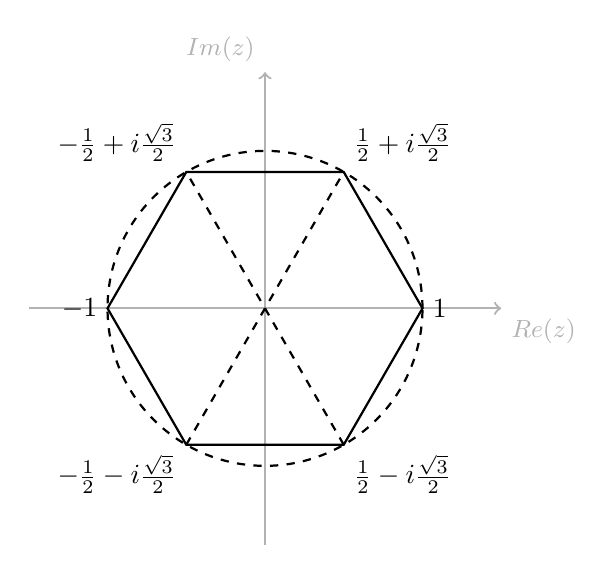
\begin{tikzpicture}[
      scale=2.0,
      axis_style/.style={draw, gray!60, thick},
      unit_circle_style/.style={draw, black, thick, dashed},
      hexagon_style/.style={draw, black, thick}
  ]

  \def\omega{1.732/2} % sqrt(3)/2, workaround the issue with sqrt() function
  \draw[axis_style, ->] (-1.5, 0) -- (1.5, 0) node[below right, font=\small] {$\text{Re}(z)$};
  \draw[axis_style, ->] (0, -1.5) -- (0, 1.5) node[above left, font=\small] {$\text{Im}(z)$};
  \draw[unit_circle_style] (0,0) circle (1);

  \draw[hexagon_style]
      (1, 0) node[right] {$1$} --
      (0.5, \omega) node[above right] {$\frac{1}{2} + i\frac{\sqrt{3}}{2}$} --
      (-0.5, \omega) node[above left] {$-\frac{1}{2} + i\frac{\sqrt{3}}{2}$} --
      (-1, 0) node[left] {$-1$} --
      (-0.5, -\omega) node[below left] {$-\frac{1}{2} - i\frac{\sqrt{3}}{2}$} --
      (0.5, -\omega) node[below right] {$\frac{1}{2} - i\frac{\sqrt{3}}{2}$} -- cycle;

  \draw[unit_circle_style] (-0.5, -\omega) -- (0.5, \omega);
  \draw[unit_circle_style] (0.5, -\omega) -- (-0.5, \omega);
  \end{tikzpicture}
  \captionof{figure}{Units of Eisenstein integers}
  \label{fig:units-of-z-omega}
\end{center}
}

\Question{Draw the lattice of Eisenstein integers of $\rho \beta$.

\vspace{2mm}
The units in above exercise span the lattice of Eisenstein integers. As shown in \cref{fig:integers-of-z-omega}, Eisenstein integers lie in the lattice of equilateral triangles. Let $\rho = m + n\omega$, where $m, n$ are integers. $\rho \beta = m\beta + n\omega\beta$. By Euler's identity, $\omega = e^{i\frac{2\pi}{3}}$, multiplying by $\omega$ is turning left by 120 degrees. Therefore, $\rho \beta$ are lattice of equilateral triangles generated by $\beta$ and the vector from rotating it by 120 degrees.

\begin{center}
  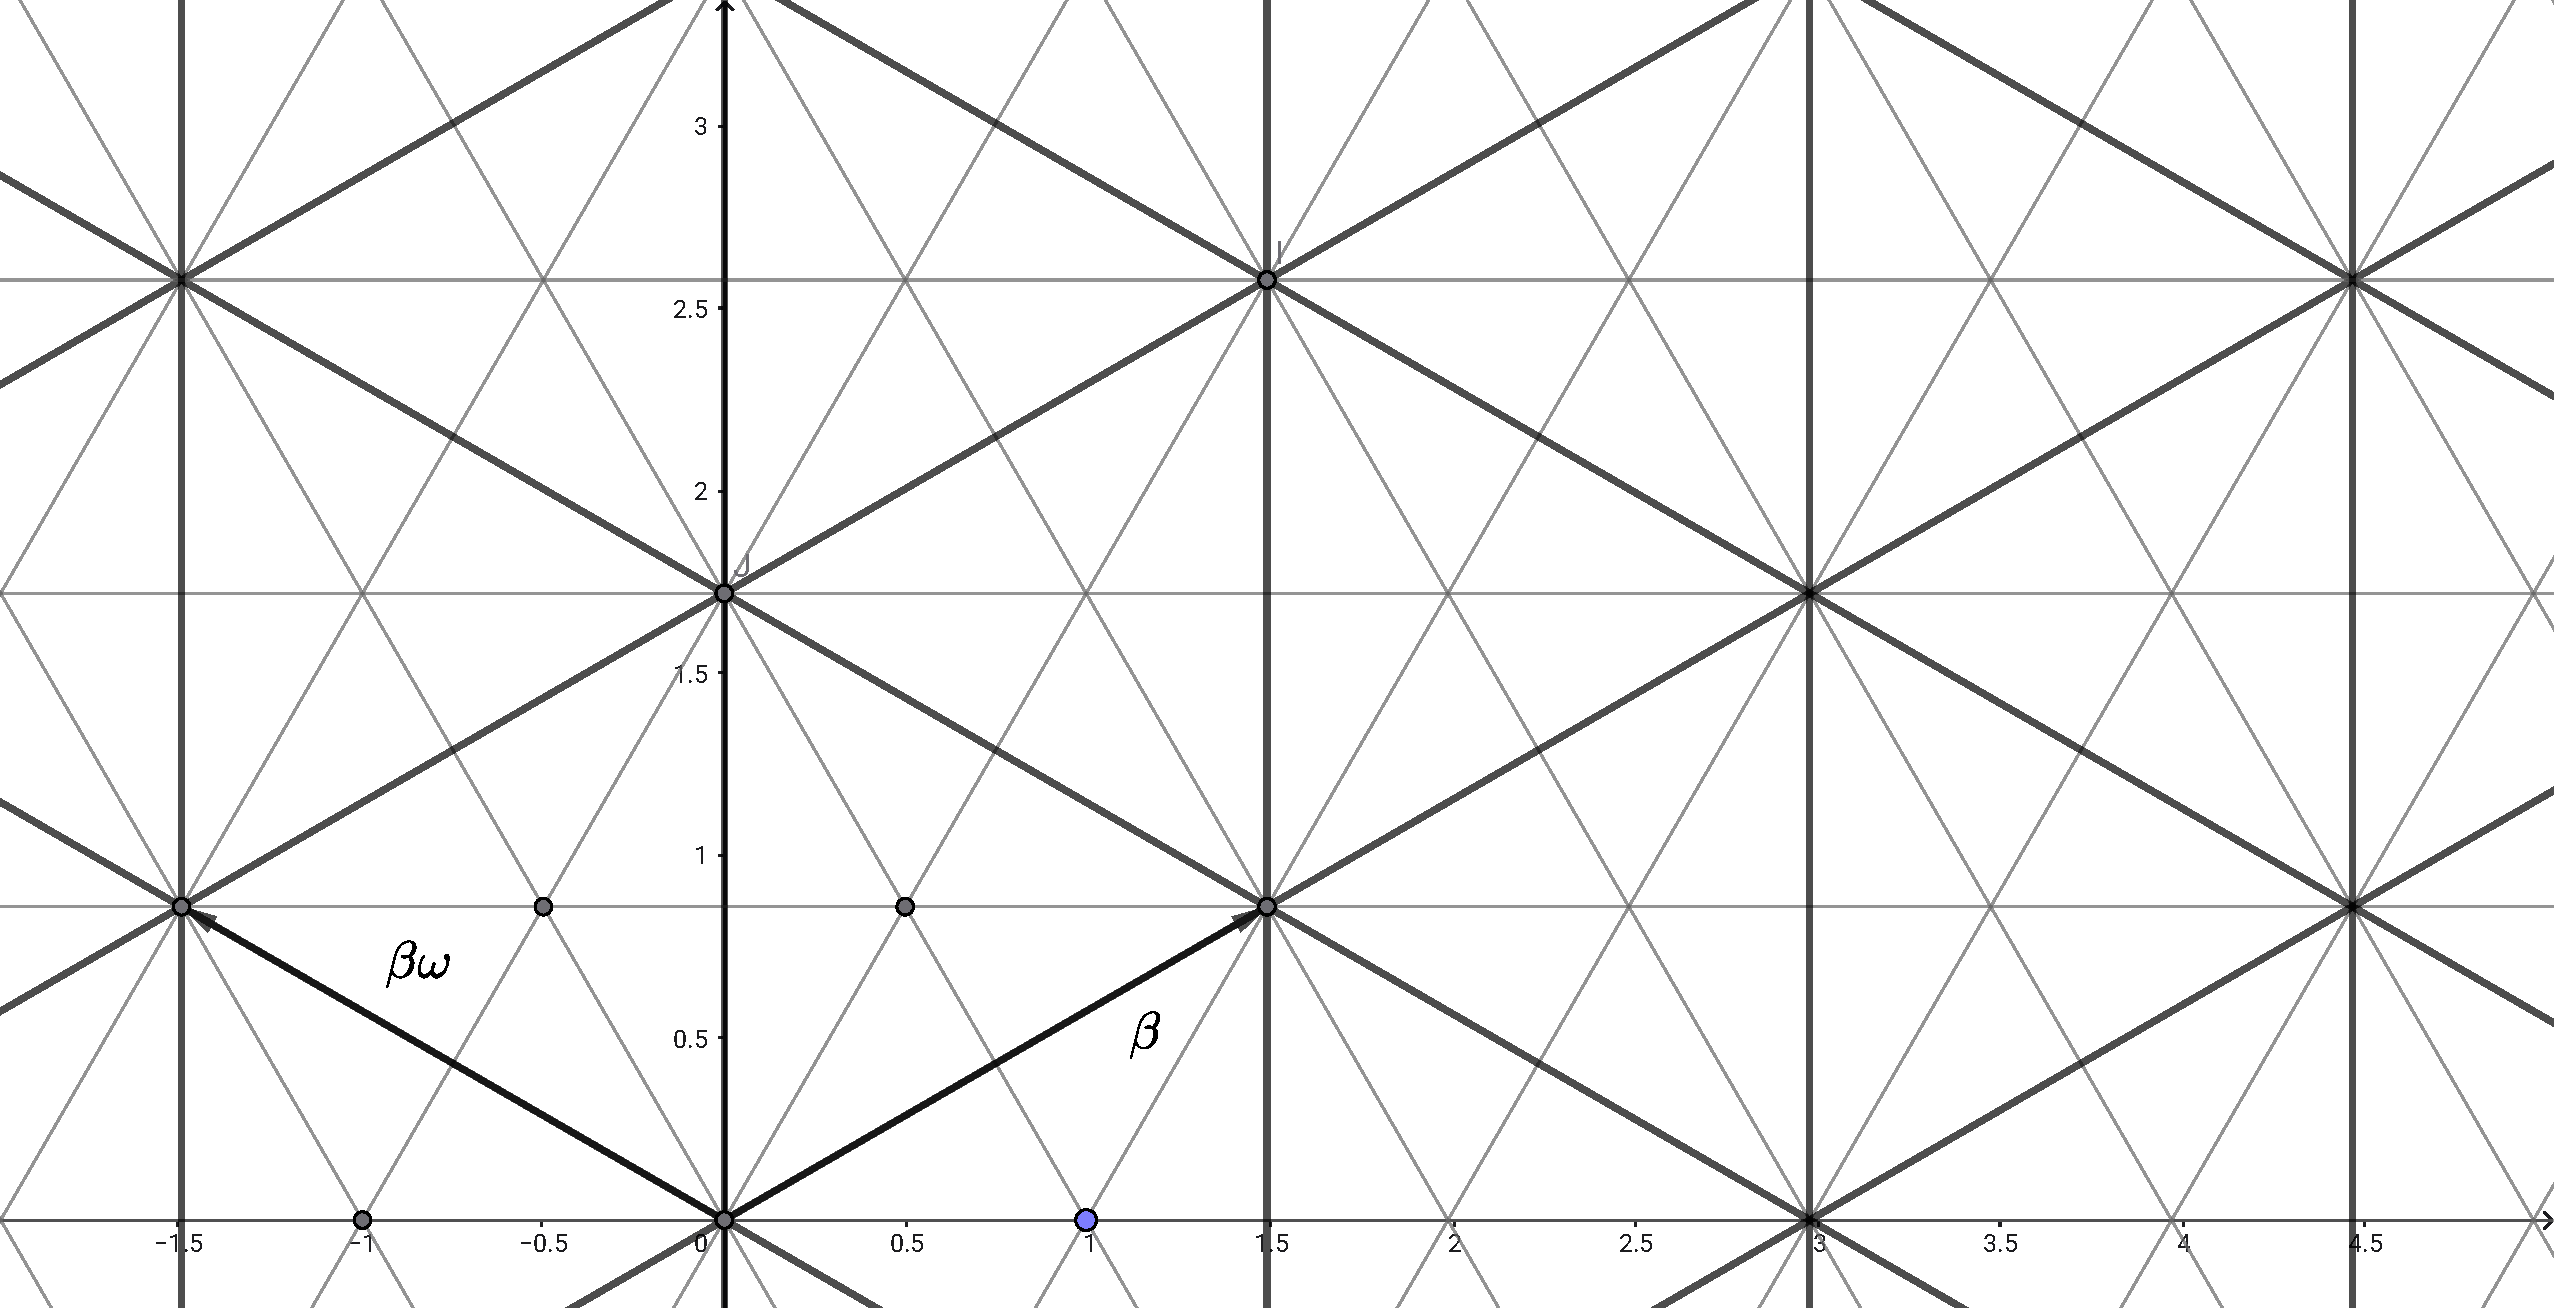
\includegraphics[scale=0.2]{img/z-omega1}
  \captionof{figure}{Eisenstein integers lie in the gray lattice of equilateral triangles; $\rho \beta$ is a similar lattice in black color.}
  \label{fig:integers-of-z-omega}
\end{center}
}

\Question{Using lattice, show that the Euclidean algorithm exists for Eisenstein integers.

\begin{center}
  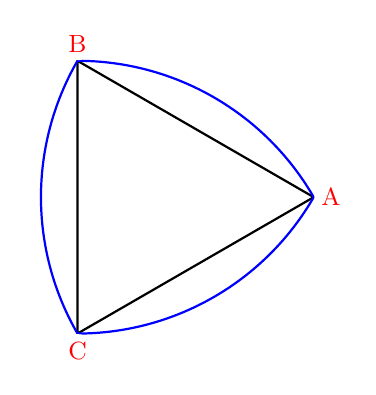
\begin{tikzpicture}[
      scale=2.0,
      triangle_style/.style={draw, black, thick},
      reuleaux_style/.style={draw, blue, thick},
      vertex_style/.style={fill, red, circle, inner sep=2pt},
      label_style/.style={font=\small, fill=white, inner sep=1pt}
  ]

      \def\A{(1,0)}
      \def\B{(-0.5,{1.732/2})}
      \def\C{(-0.5,{-1.732/2})}

      \draw[triangle_style] \A -- \B -- \C -- cycle;
      \draw[reuleaux_style] \A arc[start angle=30, end angle=90, radius=1.732];
      \draw[reuleaux_style] \B arc[start angle=150, end angle=210, radius=1.732];
      \draw[reuleaux_style] \C arc[start angle=-90, end angle=-30, radius=1.732];
      \fill[vertex_style] \A node[label_style, right] {A};
      \fill[vertex_style] \B node[label_style, above] {B};
      \fill[vertex_style] \C node[label_style, below] {C};
  \end{tikzpicture}

  \captionof{figure}{Reuleaux triangle and its inscribed equilateral triangle.}
  \label{fig:reuleaux}
\end{center}

\begin{proof}
There is a straightforward geometric argument. As shown in \cref{fig:reuleaux}, draw arcs at the center of each vertex of the equilateral triangle with the radius of side length. The three arcs enclose a Reuleaux triangle, in which the distance from any point to the closest vertex is less than the side length. Any Eisenstein integer $\alpha$ lies inside some equilateral triangle of side length $|\beta|$. The distance to the closest vertex is less than $|\beta|$. Let $\gamma = \alpha - \rho \beta$, then $N(\gamma) < N(\beta)$, which proves the existence of Euclidean algorithm.
\end{proof}
}

\Question{Show that $1 \pm i\sqrt{5}$ cannot be further factorized.

\begin{proof}
Suppose it can be factorized as $(a + bi\sqrt{5})(c + di\sqrt{5})$, taking norm on both sides:

\[
6 = 1^2 + 5^2 = N(1 \pm i\sqrt{5}) = N(a + bi\sqrt{5})N(c + di\sqrt{5}) = (a^2 + 5b^2)(c^2 + 5d^2）
\]

We rule out the case $a^2 + 5b^2 = 2, c^2 + 5d^2 = 3$ since there is no solution of $a, b, c, d$ in integers. Hence $a^2 + 5b^2 = 1$ or $c^2 + 5d^2 = 1$. The norm of 1 corresponds to unit, and the other is associate, which shows $1 \pm i\sqrt{5}$ cannot be further factorize.
\end{proof}
}

\Question{Show that the sum of ideals is an ideal.

\begin{proof}
Let $I = I_1 + I_2 = \{a + b | a \in I_1, b \in I_2\}$, we are going to show $I$ is closed under addition and scaling. For any $c_1 = a_1 + b_1, c_2 = a_2 + b_2$ in $I$, where $a_1, a_2 \in I_1, b_1, b_2 \in I_2$. Since $I_1$ is an ideal, the sum $a_1 + a_2$ is in $I_1$, let $a_3 = a_1 + a_2 \in I_1$. Similarly, the sum $b_1 + b_2$ is in $I_2$, let $b_3 = b_1 + b_2 \in I_2$.

\begin{align*}
c_1 + c_2 &= a_1 + b_1 + a_2 + b_2 = (a_1 + a_2) + (b_1 + b_2) \\
  &= a_3 + b_3 \in I && \text{where } a_3 \in I_1, b_3 \in I_2
\end{align*}

It shows the addition is close. For any $r$ in parent set $R$, any $c = a + b$ in $I$, where $a \in I_1, b \in I_2$, by the property of ideal, $ar \in I_1, br \in I_2$, therefore,

\begin{align*}
cr &= (a + b)r = ar + br \in I  && \text{where } ar \in I_1, br \in I_2
\end{align*}
It shows the scaling is close.
\end{proof}
}

\Question{For the parent set $R$ of an ideal, suppose 0 and 1 are in it, and for any element $y$ in $R$, its negative, $-y$ is also in $R$. Prove for any ideal of $R$, (1) 0 is in the ideal; (2) if $a$ is in the ideal, then $-a$ is in the ideal.

\begin{proof}
For any $a \in I, 0 \in R$, by the definition of ideal, $a \cdot 0 = 0 \in I$, which shows 0 is in any ideal. Further, $a \in I$, and since 1 is in $R$, it follows that $-1$ is in $R$. By the definition of ideal, $a \cdot (-1) = -a \in I$.
\end{proof}
}

\Question{(0) is called zero ideal, (1) is called unit ideal, what elements are in them respectively?

\vspace{2mm}
(0) has only one element, namely 0, because any multiple of 0 is still 0. (1) is the entire parent set $R$, because for any $y \in R$, it has $1y = y \in (1)$.
}

\Question{Verify that if ideal $A = (a, b) = \{ax + by | x, y \in R\}$ and ideal $B = (c, d)$, then their product $AB = (ac, ad, bc, bd)$.

\vspace{2mm}
$A = \{\alpha = ar_1 + br_2\}, B = \{\beta = cs_1 + ds_2\}$, where $r_1, r_2, s_1, s_2$ are in parent set $R$. Dedekind's definition of product of ideals can be summarized as the sum of finite many $\alpha\beta$.

\begin{align*}
AB &= \{ \sum \alpha\beta \} = \{ \sum (ar_1 + br_2)(cs_1 + ds_2) \} \\
  &= \{ \sum (acr_1s_1 + adr_1s_2 + bcr_2s_1 + bdr_2s_2) \} \\
  &= \{ ac\sum (r_1s_1) + ad\sum (r_1s_2) + bc\sum (r_2s_1) + bd\sum (r_2s_2) \} \\
  &= \{ ac S_1 + ad S_2 + bc S_3 + bd S_4 \} && \text{where }S_i = \sum (r_js_k) \\
  &= (ac, ad, bc, bd)
\end{align*}
}

%% 下面的问题本质是因为Z[\sqrt{-3}]不是Dedekind domain。所以不存在理想的唯一分解。参考：
%% https://math.stackexchange.com/questions/958030/ideals-dedekind-domain-and-mathbbz-sqrt-3
%%
%% \Question{*无法用理想解决$4 = 2 \times 2 = (1 + i\sqrt{3})(1 - i\sqrt{3})$的唯一分解。

%% \vspace{2mm}
%% 构造理想$I = (2, 1 + i\sqrt{3})$。首先$I \ne (2)$, 因为$I$中的$1 + i\sqrt{-3} \notin (2)$。但是：

%% \begin{align*}
%% A = I^2 &= (4, 2 + 2i\sqrt{3}, (1 + i\sqrt{3})^2) \\
%%         &= (4, 2 + 2i\sqrt{3}, -2 + 2i\sqrt{3}) && \text{其中} (1 + i\sqrt{3})^2 = -2 + 2i\sqrt{3}
%%         &= (2)(2, 1 + i\sqrt{-3}) = (a)I
%% \end{align*}

%% 这说明$A = I^2 = (2)I$有两种分解：(1) 素理想I^2；(2) 非素理想(2)和素理想I的积。
%% }

\Question{We establish 1-to-1 correspondence between rooms and guests as shown in \cref{fig:NNtoN}. Which room is the guest $j$ of group $i$ checked in? Conversely, which guest of which group is checked in room $k$?

\vspace{2mm}
We count from zero, denote guest $j$ of group $i$ by pair $(i, j)$. Below table list the first several mapping between guests and rooms:

\vspace{3mm}
\begin{adjustbox}{max width=\linewidth}
\begin{tabular}{c|c|c|c|c|c|c|c|c|c|c|c}
$(i, j)$ & (0, 0) & (0, 1) & (1, 0) & (2, 0) & (1, 1) & (0, 2) & (0, 3) & (1, 2) & (2, 1) & (3, 0) & ... \\
\hline
$k$ & 0 & 1 & 2 & 3 & 4 & 5 & 6 & 7 & 8 & 9 & ... \\
\hline
$i + j$ & 0 & 1 & 1 & 2 & 2 & 2 & 3 & 3 & 3 & 3 & ... \\
\end{tabular}
\end{adjustbox}
\vspace{3mm}

Writing down the sum of $i+j$, there is a pattern: there are 1 of number 0, 2 of number 1, 3 of number 2, 4 of number 3, ... these are exactly the triangle numbers discovered by the Pythagoreans. Let $m = i + j$, there are total $\frac{m(m + 1)}{2}$ grids along the diagonals on the left-bottom side of a given grid.

Along the diagonal this point belongs to, if $m$ is odd, then the room number increases along the left up direction, $i$ increases, and $j$ decreases; if $m$ is even, then the direction is right-bottom. Summarize the two cases:

\[
k = \dfrac{m(m + 1)}{2} + \begin{cases} m - j &\text{$m$ is odd} \\
j &\text{$m$ is even}
\end{cases}
\]

Further, we use $(-1)^m$ to simplify the conditions:

\[
k = \dfrac{m(m + 2) + (-1)^m (2j - m)}{2}
\]
}

\Question{There are other solutions to the story of Hilbert's Grand hotel on the third day. \Cref{fig:PWW-NNtoN} shows the cover page of \emph{proof without word}. Give a numbering scheme based on this figure.
\begin{center}
 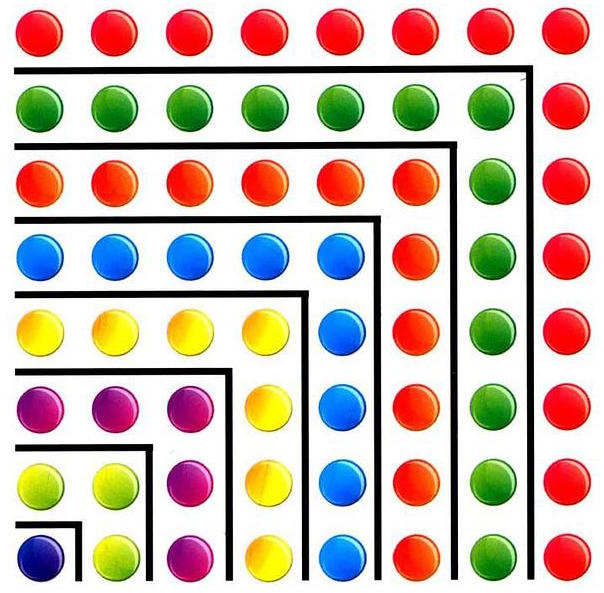
\includegraphics[scale=0.18]{img/PWW}
 \captionof{figure}{From cover page of \emph{Proof without word}}
\end{center}

\begin{center}
\begin{tikzpicture}
  \draw[step=1, very thin, gray] (0, 0) grid (5, 5);
  \draw[->] (-0.25, 0) -- (6, 0) coordinate (x axis);
  \draw[->] (0, -0.25) -- (0, 6) coordinate (y axis);
  \foreach \x in {0, 1, 2, 3, 4, 5}
    \path (\x, -0.25) node[left] {\x};
  \foreach \y in {1, 2, 3, 4, 5}
    \path (-0.25, \y) node[below] {\y};
  \foreach \i / \x / \y in {0/0/0, 1/1/0, 2/1/1, 3/0/1, 4/0/2, 5/1/2, 6/2/2, 7/2/1, 8/2/0, 9/3/0, 10/3/1}{
    \path (\x, \y) coordinate (N\i);
    \fill (N\i) circle (1pt) node[above right=3pt of N\i] {\i};
  }
  \foreach \i in {0,...,9} {
    \pgfmathsetmacro{\j}{\i+1}
    \draw[-latex, thick] (N\i) to (N\j);
  }
\end{tikzpicture}
\captionof{figure}{Alternative numbering scheme for infinity of infinity}
\label{fig:NNtoN2}
\end{center}

As shown in \cref{fig:NNtoN2}, count along the gnomon shaped path. There are odd number of grid points along every gnomon.
}
\end{Answer}

\ifx\wholebook\relax \else
\section{Answers}
\shipoutAnswer

\subimport{inc/}{fibonacci-zh-cn}
\subimport{inc/}{wilson-zh-cn}

\begin{thebibliography}{99}
\subimport{inc/}{bib-zh-cn}
\end{thebibliography}

\expandafter\enddocument
\fi
